%%%%%%%%%%%%%%%%%%%%%%%%%%%%%%%%%%%%%%%%%%%%%%%%%%%%%%%%%%%%
\documentclass[a4paper,english]{report}    % list options between brackets

\RequirePackage[dvips]{color}
\RequirePackage{float}
\RequirePackage{amsfonts}
\RequirePackage{amsmath}
\RequirePackage{alltt}
\RequirePackage{ae}
\RequirePackage{times}
\RequirePackage{fancyheadings}
\RequirePackage{graphicx} 

\usepackage{makeidx}  
\makeindex             

%%%%%%%%%%%%%%%%%%%%%%%%%%%%%%%%%%%%%%%%%%%%%%%%%%%%%%%%%%%%

\newcommand{\Sf}[1]{\textsf{#1}}
\newcommand{\Bf}[1]{{\sffamily\bfseries}}
\newcommand{\Bfm}[1]{\mbox{\boldmath{${#1}$}}}
\newcommand{\URL}[1]{\texttt{#1}}

% Some new commands...
\def\xwin{X Window System}
\def\xbr{Xbrowse}
\def\prag{\Tt{\#pragma}}

\newcommand{\inxgra}[2]{{\centerline{\includegraphics[width=#1]{#2}}}}
\newcommand{\inygra}[2]{{\centerline{\includegraphics[height=#1]{#2}}}}
\newcommand{\incgra}[2]{{\centerline{\includegraphics[height=#1]{#2}}}}

\providecommand{\ftn}{Fort\-ran~90}
\providecommand{\Idx}[1]{{#1}\index{#1}}

\newcommand{\ttbegin}{\begin{alltt}}
\newcommand{\ttend}{\end{alltt}}
\newcommand{\keno}{$\backslash$}
%%%%%%%%%%%%%%%% Definitions for Elmer Solver Manuals %%%%%%%%%%%%%%%%%

%\newcommand{\Vec}[1]{\mathify{\mathbf{#1}}}
%\newcommand{\Vec}[1]{\vec{#1}}
\newcommand{\Div}{\nabla\cdot}
\newcommand{\Curl}{\nabla\times}
\newcommand{\Grad}{\nabla}


\definecolor{SifCol}{rgb}{0.5,0.5,0.5}
%normal item, with text also (2 parameters + text)
\newcommand{\sifitem}[2]{\item[\tt{#1}]\hspace{1mm}{\color{SifCol}\hspace{1mm}\tt{#2}}\newline} 
%item with two fields but no text
\newcommand{\sifitemnt}[2]{\item[\tt{#1}]\hspace{1mm}{\color{SifCol}\hspace{1mm}\tt{#2}}} 
\newcommand{\sifbegin}{\begin{description}}
\newcommand{\sifend}{\end{description}}
\newcommand{\modinfo}[2]{{\bf{#1}}: {#2}\newline}

\newcommand{\Matr}[1]{\mbox{\boldmath{${#1}$}}}
\newcommand{\Der}[2]{\frac{\partial{#1}}{\partial{#2}}}
\newcommand{\Secder}[2]{\frac{\partial^2{#1}}{\partial{#2}^2}}
\newcommand{\Inv}[1] {\frac{1}{#1}}
%\DeclareMathOperator{\Div}{div}
%\DeclareMathOperator{\Grad}{grad}
%\DeclareMathOperator{\Curl}{curl}

% Use these to make the printable area bigger
% Also have the option 'ownsize' active in the documentclass
\setlength{\hoffset}{-15mm}
\setlength{\voffset}{-10mm}
\addtolength{\textwidth}{30mm}
\addtolength{\textheight}{20mm}
%\addtolength{\headwidth}{30mm}

% Make the headings fancier
\pagestyle{fancy}
\lhead[\normalfont\small\bf\thepage]{\normalfont\small\slshape\rightmark}
\rhead[\small\slshape\lefthead]{\normalfont\small\bf \thepage}
\setlength{\headrulewidth}{0.4pt}
%\renewcommand{\chaptermark}[1]{\markright{\bf \chaptername \ \thechapter.\ #1}{}}
\renewcommand{\chaptermark}[1]{\markright{\bf \thechapter.\ #1}{}}
\renewcommand{\sectionmark}[1]{}
\renewcommand{\subsectionmark}[1]{}
\cfoot{}


% This sets the Elmer version in the documentation
\newcommand{\elmerversion}{~5.4}



%%%%%%%%%%%%%%%%%%%%%%%%%%%%%%%%%%%%%%%%%%%%%%%%%%%%%%%%%%%%

\title{\Huge{\bf Elmer Tutorials}}
\author{CSC, the Finnish IT Center for Science}
\date{\today}

%%%%%%%%%%%%%%%%%%%%%%%%%%%%%%%%%%%%%%%%%%%%%%%%%%%%%%%%%%%%

\begin{document}
\maketitle

\chapter*{Copyrights}

This document gives practical examples of the use of Elmer,
a finite element software for multiphysical problems.
The copyright if this document and Elmer software belong to
CSC -- IT Center for Science, Finland, 1995--2008. 

Elmer program is free software; you can redistribute it and/or
modify it under the terms of the GNU General Public License
as published by the Free Software Foundation; either version 2
of the License, or (at your option) any later version.

This program is distributed in the hope that it will be useful,
but WITHOUT ANY WARRANTY; without even the implied warranty of
MERCHANTABILITY or FITNESS FOR A PARTICULAR PURPOSE.  See the
GNU General Public License for more details.

CSC assumes no responsibility or liability on any errors or inaccuracies in 
Elmer program or documentation. Any kind of material damages or other indirect
consequences resulting from any Elmer part, documentation discrepancies and 
errors or non-anticipated program behavior are limited to the value of 
appropriate products purchased from CSC. 

This document is for informational use only. All information and specifications
given have been carefully prepared by the best efforts of CSC, and are believed
to be true and accurate as of time publishing. CSC reserves the right to 
modify Elmer and its documents without notice. \\  \mbox{} \\

\textbf{Additional software product copyrights included in Elmer}

Copyright, and License:

UMFPACK Version 4.3, Jan. 16, 2004. Copyright (c) 2004 by Timothy
A. Davis, University of Florida, davis@cise.ufl.edu. All Rights
Reserved. 


UMFPACK License: 

Your use or distribution of UMFPACK or any derivative code implies
that you agree to this License. 

      THIS MATERIAL IS PROVIDED AS IS, WITH ABSOLUTELY NO WARRANTY
      EXPRESSED OR IMPLIED. ANY USE IS AT YOUR OWN RISK. 

      Permission is hereby granted to use or copy this program,
      provided that the Copyright, this License, and the Availability
      of the original version is retained on all copies. User
      documentation of any code that uses UMFPACK or any modified
      version of UMFPACK code must cite the Copyright, this License,
      the Availability note, and "Used by permission." Permission to
      modify the code and to distribute modified code is granted,
      provided the Copyright, this License, and the Availability note
      are retained, and a notice that the code was modified is
      included. This software was developed with support from the
      National Science Foundation, and is provided to you free of
      charge. 


\chapter*{About ElmerGrid Manual}

The ElmerGrid Manual is part of the documentation of 
Elmer finite element software package.
ElmerGrid Manual gives instruction 
on the usage of ElmerGrid, the mesh generation and manipulation utility of Elmer.

The present ElmerGrid Manual
corresponds to software version \elmerversion{}.
The latest versions of Elmer software and its documentation
are available at the Elmer homepage at
\URL{http://www.csc.fi/elmer}. 




%%%%%%%%%%%%%%%%%%%%%%%%%%%%%%%%%%%%%%%%%%%%%%%%%%%%%%%%%%%%

%\pagenumbering{roman}
\pagestyle{empty}

% Table of contents:
\setcounter{secnumdepth}{2}
\setcounter{tocdepth}{1}  % set this to 1 in the final version

\tableofcontents

%%%%%%%%%%%%%%%%%%%%%%%%%%%%%%%%%%%%%%%%%%%%%%%%%%%%%%%%%%%%

\newpage
\renewcommand{\chaptername}{Tutorial}
\pagestyle{fancy}

% Change the left page header text
\providecommand{\lefthead}{Elmer Tutorials}

%%%%%%%%%%%%%%%%%%%%%%%%%%%%%%%%%%%%%%%%%%%%%%%%%%%%%%%%%%%%

\clearpage
\pagenumbering{arabic}

\part{Simple Problems}

\graphicspath{{./}{TemperatureAngle/}}
\chapter{Operator Splitting Ability}

\modinfo{Solvers}{\Idx{HeatSolve}} 
\modinfo{Tools}{\Idx{ElmerFront}} 
\modinfo{Dimensions}{2D, Steady-state}

\subsection*{Problem description}

An L-shaped structure (see figure~\ref{fg:struct1}) is heated by an internal 
heat source magnitude of which is 1 W/m$^3$. The density of the structure 
material is 1 kg/m$^3$ and its heat conductivity is 1 W/mK. All the 
boundaries $\Gamma_i$ are kept on constant temperature of 0 K. The problem is 
to solve the temperature distribution in the structure.

\begin{figure}
\begin{center}
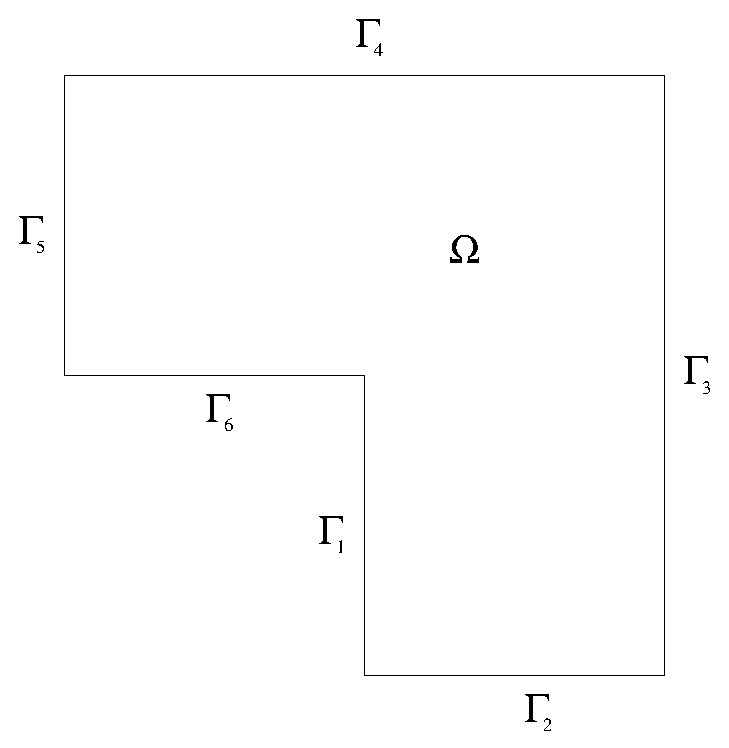
\includegraphics[width=60mm]{Area1}
\caption{L-shaped structure}\label{fg:struct1}
\end{center}
\end{figure}

Mathematically the problem to be solved is
\begin{equation}
\left \{
\begin{array}{cccc}
- \kappa \Delta T &= &f & \mbox{ in } \Omega \\
T&=&0 & \mbox{ on } \Gamma
\end{array}
\right .
\end{equation}
where $\kappa$ is the heat conductivity, $T$  is the temperature 
and $f$ is the heat source. It is assumed that density 
and heat conductivity are constants. 

\subsection*{Solution procedure}

\begin{itemize}
\item Start Elmer in the desired directory with the command
\ttbegin
ElmerFront
\ttend
\item Open the file that contains the geometry of the structure from 
the File menu. Select also the working directory for the model.
\ttbegin
File -> Open cad-file 
  File = TempDist.egf 
  Model name = TempDist 
  Model directory = split_tutorial
\ttend
\item Select the equations to be solved from the Problem menu. In this 
case there is only one equation, the heat equation. Remember to add the 
equation to the equation sets. This connects the equation to the defined 
body. 
\ttbegin
Problem ->\ldots Equations 
  Heat equation 
\ttend
\item Apply the body forces from the Model menu. Give the value for the body 
force (heat source). Remember to add the body forces to the body force 
sets so that they have an effect on $\Omega$ (see figure~\ref{fg:struct1}). 
\ttbegin
Model -> Body forces 
  Heat source = 1
\ttend
\item Define the material properties from the Model menu. Give the values for 
the density and the heat conductivity. Add the defined material properties 
to the material property sets so they become attached to $\Omega$. 
\ttbegin
Model -> Materials 
  Density = 1 
  Heat conductivity = 1
\ttend
\item Define boundary conditions from the Model menu. Give the value of the 
temperature at the boundaries $\Gamma_i$. Add the defined boundary condition 
to boundary condition sets and attach the constraint to all the boundaries 
$\Gamma_i (i=1,\ldots,6)$ of $\Omega$ (see figure~\ref{fg:struct1}). 
\ttbegin
Model -> Boundary conditions 
  Temperature = 0 
\ttend
\item Define mesh for the structure from the Mesh menu. First give name for 
the mesh and then define the element size. Make the mesh by pressing
``Generate mesh'' button. 
\ttbegin
Mesh -> Define mesh 
  Mesh name = Mesh1 
  Model Mesh H [m] = 0.1 
  Generate mesh
\ttend
\item Now to solve the problem select from the Run menu item Solver. This 
starts the solver. 
\ttbegin
Run -> Solver 
\ttend
\item After the solution is done, view the results by selecting from the Run
menu item Postprocessor. 
\ttbegin
Run -> Postprocessor 
\ttend
\item To save the created model, select from the File menu item Save 
model file. 
\ttbegin
File -> Save model file 
\ttend
\item To exit Elmer select from the File menu item Exit. 
\ttbegin
File -> Exit
\ttend
\end{itemize}

\subsection*{Results}

As a result a maximum temperature in the structure is given. For a 
comparison the same problem was solved six times with different 
element sizes. The maximum temperature obtained
by using different meshes is recorded in table~\ref{tb:struct1}.
From the results you can see that the result converges. With a denser mesh 
the result is more accurate, but it takes more calculation time. 

\begin{table}
\caption{Results with different element sizes}
\label{tb:struct1}
\begin{center}
\begin{tabular}{lll} \hline
Model Mesh H [m]  & Elements & $\max (T)$ [K] \\ \hline
0.2 & 186 &  0.14267 \\ 
0.15 & 326 & 0.1462  \\ 
0.1 &  726 & 0.14788 \\
0.05 & 2 792 & 0.1487  \\ 
0.025 & 11 078 & 0.14919  \\ 
0.01  & 69 642 & 0.14935 \\ \hline
\end{tabular}
\end{center}
\end{table}






\graphicspath{{./}{TemperatureRadiation/}}
\chapter{Radiation heat transfer}

\modinfo{Directory}{\Idx{TemperatureRadiation}}
\modinfo{Solvers}{\Idx{HeatSolve}}
\modinfo{Tools}{\Idx{ElmerGrid}, editor}
\modinfo{Dimensions}{2D, Axi-Symmetric}

\subsection*{Case definition}

At high temperature the radiation heat transfer between walls 
is often the dominating heat transfer mechanism. In this
tutorial we look how radiation heat transfer between 
cocentric cylinders is modeled. 


\subsection*{Solution Procedure}

The problem is a pure heat transfer problem that may be solved
with \texttt{HeatSolve}. The view and Gebharht factors 
associated with the radiation are solved as a first step 
in solving the equations. Thereafter the nonlinear heat equation is solved
until convergence is reached.

The computatonal mesh is done with \texttt{ElmerGrid} in directory \texttt{radiation} 
with the command 
\ttbegin
ElmerGrid 1 2 radiation
\ttend
The directory is given in the header of the command file
\ttbegin
Header
  Mesh DB "." "radiation"
End
\ttend
%
The only constant required is the Stefan-Boltzmann constant that gives the
relationship between temperature and radiation power
\ttbegin
Constants
  Stefan Boltzmann = 5.67e-8
End
\ttend
%
The geometry is axisymmetric and the case is solved in steady state.
As there is only one equation only 1 iteration for the system is required.
\ttbegin
Simulation
  Coordinate System = Axi Symmetric
  Simulation Type = Steady State
  Steady State Max Iterations = 1
  Output Intervals = 1
  Output File = "radiation.result"
  Post File = "radiation.ep"
End
\ttend
% 
There are two bodies with the same equation but different properties.
\ttbegin
Body 1
  Equation = 1
  Body Force = 1
  Material = 1
  Initial Condition = 1
End

Body 2
  Equation = 1
  Material = 2
  Initial Condition = 1
End
\ttend
%
The nonlinear equation requires realistic initial conditions. Otherwise convergence
may not be obtained.
\ttbegin
Initial Condition 1
  Temperature = 250.0
End
\ttend
The body force is the heating power in units W/kg. 
\ttbegin
Body Force 1
  Heat Source = 10000
End
\ttend
The material properties differ only in heat conductivity. Heat capacity is not
actually needed since the case is not transient.�
\ttbegin
Material 1
   Density = 1.0
   Heat Conductivity = 10.0
   Heat Capacity = 1.0
End

Material 2
   Density = 1.0
   Heat Conductivity = 1.0
   Heat Capacity = 1.0
End
\ttend
The heat equation is solved with an itrative procedure that requires some relaxation 
for better convergence. There are two different ways to discretize the radiation. 
There are two keywords defining when to switch to the true Newtonian iteration
which should give better convergence.
\ttbegin
Solver 1
  Equation = Heat Equation
  Stabilize = True
  Linear System Solver = Iterative
  Linear System Iterative Method = BiCGStab
  Linear System Convergence Tolerance = 1.0e-12
  Linear System Max Iterations = 500
  Linear System Preconditioning = ILU
  Nonlinear System Newton After Iterations = 1
  Nonlinear System Newton After Tolerance = 1.0e-4
  Nonlinear System Max Iterations = 50
  NonLinear System Convergence Tolerance = 1.0e-8
  Steady State Convergence Tolerance = 1.0e-8
  Nonlinear System Relaxation Factor = 0.7
End
\ttend
The only solver is the heat equation.
\ttbegin
Equation 1
  Active Solvers = 1
End
\ttend
%
The radiation boundary conditions are set for two different boundaries. The first one
is for the internal object and the second one for the insulation. The normal direction
of the surfaces is important since a wrong direction may result to badly set problem for
the view factor computation. Internal and external surfaces are very different.
The normal direction may be switched with the keyword \texttt{Radiation Target Body}.
A good sign of properly set case is that the view factors add up to about one.
\ttbegin
Boundary Condition 1
   Target Boundaries = 1
   Heat Flux BC = True
   Radiation = Diffuse Gray
   Radiation Target Body = -1
   Emissivity = 0.6
End

Boundary Condition 2
   Target Boundaries = 2
   Heat Flux BC = True
   Radiation = Diffuse Gray
   Radiation Target Body = -1
   Emissivity = 0.1
End
\ttend
%
The third boundary condition is the Dirichtlet condition for the extranal boundary.
Dirichtlet conditions boost up the convergence even though the heat equation is basically
well defined also with external radiation conditions.
\ttbegin
Boundary Condition 3
   Target Boundaries = 3
   Temperature = 100.0
End
\ttend


\subsection*{Results}

\begin{figure}
\begin{center}
  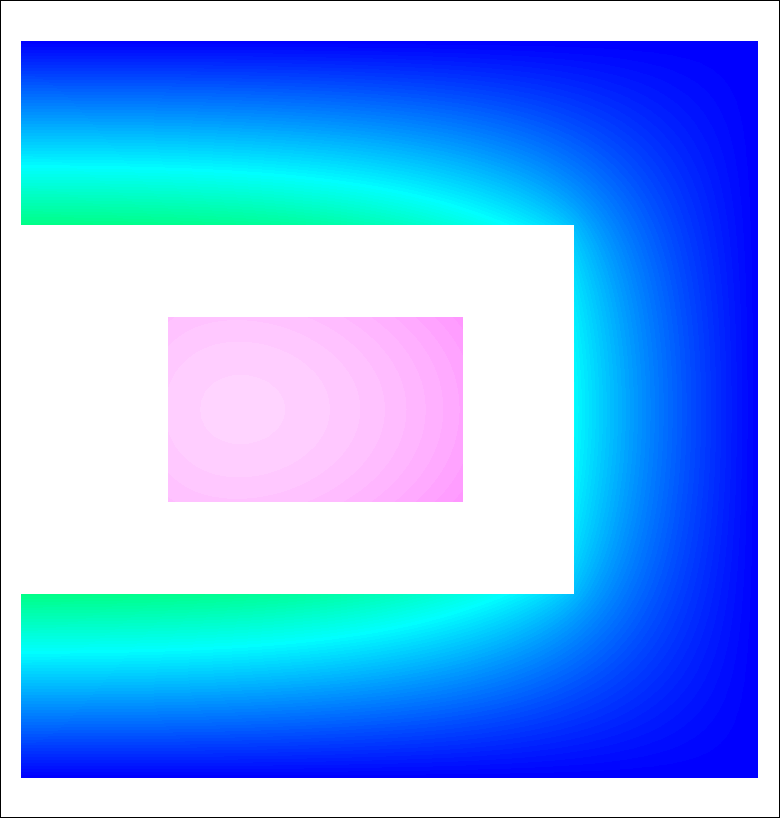
\includegraphics[height=0.6\textwidth]{radiation}
\end{center}
\caption{Temperature distribution in the radiation heat transfer
problem}
\label{fig:temp_rad1}
\end{figure}
 
With the given computational mesh the problem is solved in 
around 30 seconds. With 1\,231 second order 9-noded
rectangular elemenets the maximum temperature is 565.7~K.
The corresponding results are shown
in Fig.~\ref{fig:temp_rad1}.

\hfill

\graphicspath{{./}{ElasticBeam/}}
\chapter{Loaded elastic beam}

\modinfo{Directory}{ElasticBeam}

\section{Solution with linear model} 


\modinfo{Solvers}{\Idx{StressSolve}}
\modinfo{Tools}{\Idx{ElmerFront}}
\modinfo{Dimensions}{2D, Steady-state}

\subsection*{Case definition}

A homogenous, elastic beam ($\Omega$) is rigidly supported on one 
end (boundary $\Gamma_4$). On boundary $\Gamma_3$ the beam is subjected 
to a load $q(x)$, which grows linearly from zero to $q_0$ 
(see figure~\ref{fg:beam}). Material properties of the beam are the Poisson 
ratio 0.3 and Young's modulus $200\cdot 10^9$N/m$^2$. Problem is to solve the 
displacement of the beam.  

\begin{figure}[h]
\centering
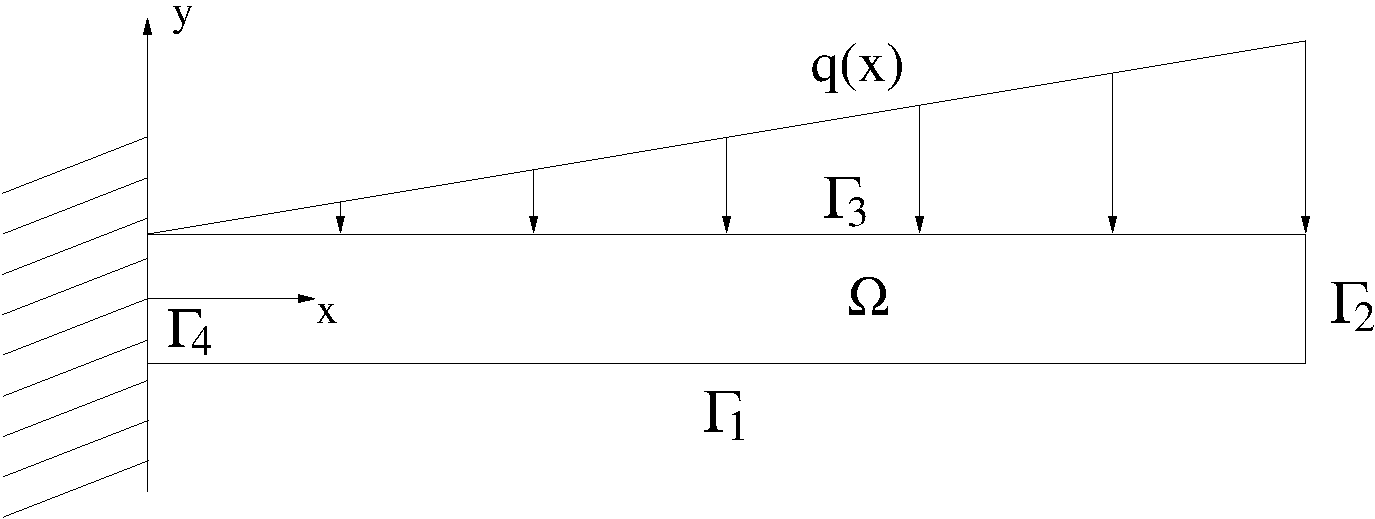
\includegraphics[width=100mm]{Beam}
\caption{Beam and loading.}\label{fg:beam}
\end{figure}

Problem is solved according to linear elasticity theory. Mathematically 
the problem to be solved is
\begin{equation}
\left \{
\begin{array}{rcll}
-div \sigma & = & 0 & \mbox{ in } \Omega \\
\sigma & = & \lambda tr [\varepsilon(u)]I + 2 \mu \varepsilon(u) &
\mbox{ in } \Omega \\
u & = & 0 & \mbox{ on } \Gamma_4 \\
\sigma n & = & 0 & \mbox{ on } \Gamma_1 \cup \Gamma_2 \\
\sigma n & = & -q & \mbox{ on } \Gamma_3 \\
\end{array}
\right .
\end{equation}
where $\lambda$ and $\mu$ are the Lam\'{e} constants (which can be expressed 
in terms of the Poisson ratio and Young's modulus), $\varepsilon$ is the 
linearized strain tensor, $u$ is the displacement vector, $q$ is the given
surface traction and $n$ is the outward unit normal to the boundary.

\subsection*{Solution procedure}

\begin{itemize}
\item Start ElmerFront.
\item Open the file that contains the geometry of the beam from 
the File menu. Select also the working directory for the model.
\ttbegin
File -> Open cad-file 
  File = Beam.egf 
  Model name = Beam 
  Model directory = beam_tutorial
\ttend
\item Select the equations to be solved from the Problem menu. In this 
case stress analysis is selected. It solves the problem according to 
linear elastic theory. 
\ttbegin
Problem -> Equations 
  Stress analysis 
\ttend
\item Define the material properties from the Model menu. Give the values for 
Young's modulus and the Poisson ratio. Add the defined material 
properties to the material property sets so they become attached 
to $\Omega$. 
\ttbegin
Model -> Materials 
  Young's modulus = 200e9 
  Poisson ratio = 0.3
\ttend

\item Define the Dirichlet boundary condition and the load from the
Model menu. Give the value zero for displacements at the boundary
$\Gamma_4$ and press Add. The linearly varying load is defined in the
same panel as follows.  Select the boundary~3, click the cursor on to
the Force-y line, check the box Table, and press finally the Edit
button. A window opens in which the tabular bc entry is
defined. Select first Coordinate 1 as the variable on which the
Force-y depends. Write on the line below entry {\tt 0 0}. Click
Add. Write {\tt 1 -1.0e7} on the line and click again Add. Now, the
space below contains two lines written in two columns. The first
colums holds the values for the Coordinate~1 and the second column for
the Force-y. The value of the force is interpolated according to these
definitions. Now click OK on the Table entry panel. In Boundary
Conditions panel, click Add and then OK.
\ttbegin
Model -> Boundary conditions
Boundary 4
Displacement-X = 0
Displacement-Y = 0
Add
Boundary 3
Force-Y
Table
Edit
Variable = Coordinate 1
0 0
Add
1 -1e7
Add
OK
Add
OK
\ttend

\item Define mesh from the Mesh menu. First give name for the
mesh. Then select ``Mesh structure'' and define element type and the
number of elements. Attach the defined mesh structure to the Body~1
and click OK. Create the mesh by pressing ``Generate mesh'' button.

\ttbegin 
Mesh -> Define mesh 
Mesh name = Mesh1 
Mesh structure 
Element type = Quad 
Nof elements (1st and 3rd edge) = 40 
Nof elements (2nd and 4th edge) = 4 
Add 
OK 
Generate mesh 
\ttend
\item Now to solve the problem defined with the constant load select from 
the Run menu item Solver. 
\ttbegin
Run -> Solver 
\ttend
\item Results may be viewed with the ElmerPost program
\ttbegin
Run -> Postprocessor
\ttend
or click the {\tt Results} button on the main window.
\end{itemize}

\subsection*{Results}

As a result the absolute value of maximum displacement is given. The 
displacements calculated with different load values $q_0$ are tabulated in 
table~\ref{tb:struct3a}. Note that the absolute value of the
displacement varies linearly with respect to the load since the model
is linear.

\begin{figure}[h!]
\begin{center}
  
\includegraphics[width=0.30\textwidth,angle=0]{respic1.png}
  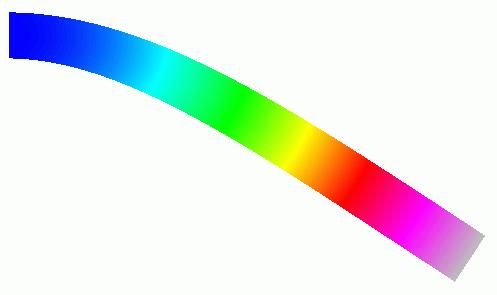
\includegraphics[width=0.28\textwidth,angle=0]{respic2.png}
  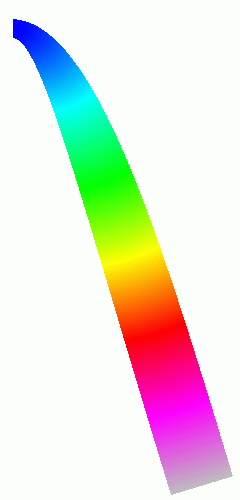
\includegraphics[width=0.25\textwidth,angle=0]{respic3.png}
  \caption{The displacement of an elastic beam with different loads
using a linear model}
  \label{fig:elast_beam1}
\end{center}
\end{figure}

\begin{table}[h]
\caption{Displacements with different load values}
\label{tb:struct3a}
\begin{center}
\begin{tabular}{ll} \hline
$q_0$ [N/m$^2$] & $\max |u|$ [m] \\ \hline
-1.0$e7$ & 0.04862 \\
-1.0$e8$ & 0.4862 \\
-1.0$e9$ & 4.862 \\ \hline
\end{tabular}
\end{center}
\end{table}

If you look at the results you can see that the displacement values
become relatively large. The linear theory is valid only to small 
displacements. From Fig~\ref{fig:elast_beam1} you can also notice that the
beam does not maintain its original form. This means that the linear 
elasticity theory can not take into consideration all the necessary 
phenomenona that are related to the problem, anymore. To be able to 
solve the problem we must use general elasticity theory. This is done 
in the following subsection.


\section{Solution with nonlinear model}

\modinfo{Solvers}{\Idx{ElasticSolve}}
\modinfo{Tools}{editor}
\modinfo{Dimensions}{2D, Steady-state}

\subsection*{Case definition}

In the following the beam problem is solved with general elasticity theory.
That is done by using the nonlinear elasticity solver of Elmer. 
In the case of homogenous 
elastic material the problem can be written into a following mathematical form

\begin{equation}
\left \{
\begin{array}{rcll}
-div [(I+ \nabla u) \Sigma] & = & 0 & \mbox{ in } \Omega \nonumber \\
\Sigma & = & \lambda (tr E)I + 2 \mu E & \mbox{ in } \Omega \nonumber \\
E & = & \frac{1}{2}(\nabla u^{T} + \nabla u + \nabla u^{T} \nabla u) & 
\mbox{ in } \Omega \nonumber \\
u & = & 0 & \mbox{ on } \Gamma_4 \\
(I+ \nabla u)\Sigma n & = & 0 & \mbox{ on } \Gamma_1 \cup \Gamma_2 \\
(I+ \nabla u)\Sigma n & = & -q & \mbox{ on } \Gamma_3 \\
\end{array}
\right .
\end{equation}
where $u$ is the displacement vector, $q$ is the given surface load, $\Sigma$ 
is the second Piola-Kirchhoff stress tensor, $\lambda$ and $\mu$ are the 
Lam\'{e} constants and $E$ is the Green-St Venant strain tensor.


\subsection*{Solution procedure}

The problem is solved here without the graphical user interface.
Open the solver input file of the linear case, Beam.sif, and edit the
following changes. Define nonlinear elasticity as the only equation
\ttbegin
Equation 1
  Name = "Equation1"
  Nonlinear Elasticity = Logical True
End
\ttend

Change the name correspondingly in the Solver block and add
information about the procedure needed. Leave all other keywords on
the solver block unchanged.
\ttbegin
Solver 1
  Equation = "Nonlinear Elasticity"
  Procedure = "ElasticSolve" "ElasticSolver"
...
End
\ttend

Finally, the force load may be changed in boundary condition 2 as
\ttbegin
  Force 2 = Variable Coordinate 1
      0 0
      1 -1.0000e+09
    End
\ttend

The problem may now be solved from the command line by typing {\tt
ElmerSolver}.

\subsection*{Results}

\begin{table}[tbhp]
\caption{Maximum displacements with different load values calculated according to 
general elasticity theory and linear theory.}
\label{tb:struct3b}
\begin{center}
\begin{tabular}{lll} \hline
$q_0$ [N/m$^2$] & 
$\max |u|$ [m] &
$\max |u|$ (linear) [m] \\ \hline
-1.0e$^7$ & 0.04890 & 0.04862 \\
-1.0e$^8$ & 0.4532 & 0.4862  \\
-1.0e$^9$ & 1.297  & 4.861 \\ \hline
\end{tabular}
\end{center}
\end{table}

From table~\ref{tb:struct3b} you can see the difference between the 
results calculated according to nonlinear and linear theory. According to 
the linear theory the displacement increases linearly as the load 
increases. This can be seen clearly from the results. The last loading
level (-1.0e9 N/m$^2$) is fairly large and the beam would probably break 
under that load. So the value of displacement might be unrealistic in that
case.   


\vfill
\mbox{}


\graphicspath{{./}{ElasticEigenValues/}}
\chapter{Eigenvalue analysis of an elastic beam}

\modinfo{Directory}{\Idx{ElasticEigenValues}}
\modinfo{Solvers}{\Idx{StressSolve}, \Idx{EigenSolve}}
\modinfo{Tools}{\Idx{ElmerGrid},Editor}
\modinfo{Dimensions}{3D, Steady-state}

\subsection*{Case definition}

A homogenous, elastic silicon beam of dimensions 1 m length, 0.1 m height and 0.2 m width
is supported on its both ends (boundaries 1 and 2). 
A beam has the density 2330 kg/m$^{3}$, Poisson ratio 0.3 and Young's modulus 10$^{11}$ N/m$^{2}$. The problem is to calculate the eigenvalues of the beam. Mathematically the equation to be solved is
\begin{displaymath}
-\rho \omega^{2}\phi = \nabla\cdot\tau(\phi)
\end{displaymath}
where $\rho$ is the density, $\omega$$^{2}$ is the eigenvalue, $\omega$ is the angular frequency, $\phi$ is the corresponding vibration mode and $\tau$ is the stress tensor.

\begin{figure}[h]
\centering
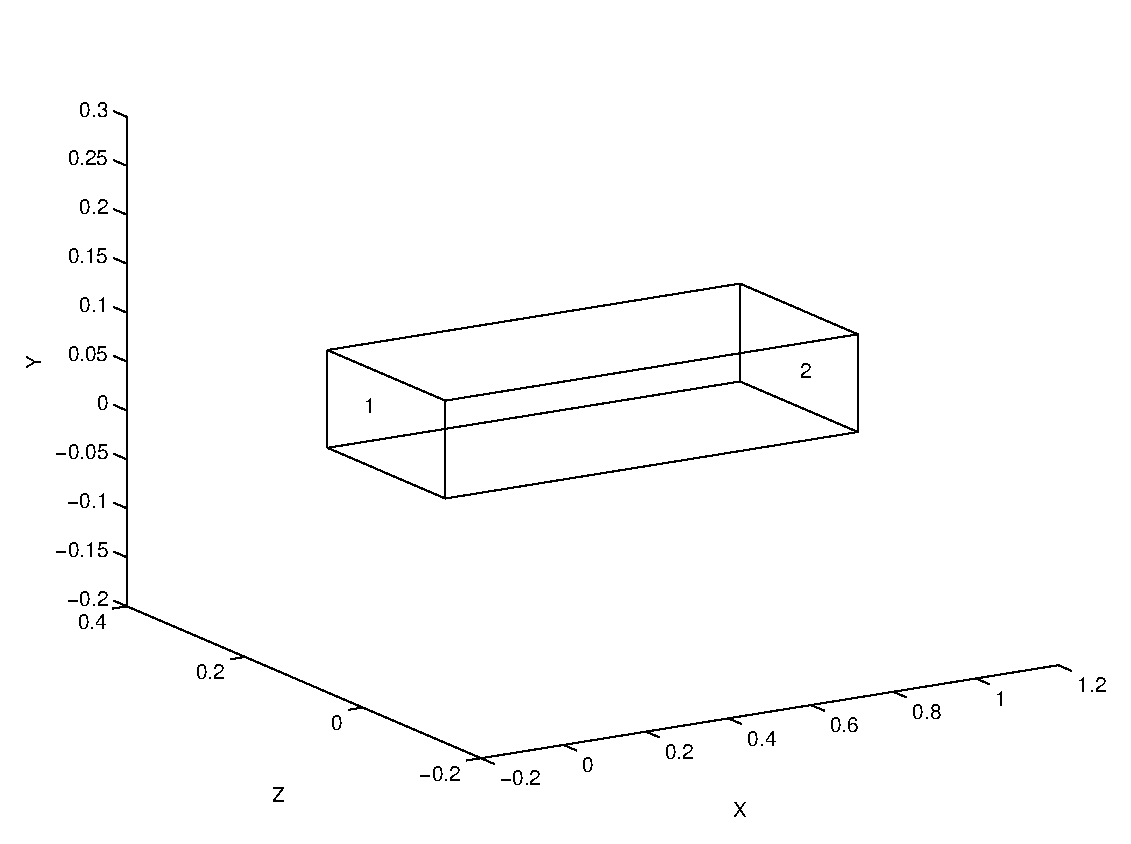
\includegraphics[height=80mm]{palkki}
\caption{Beam.}\label{fg:palkki}
\end{figure}




\subsection*{Solution procedure}

The mesh has been created by using Gambit software and it consists of 2500 elements. The mesh can be converted to Elmer format with ElmerGrid with the command

\ttbegin
ElmerGrid 7 2 mesh.FDNEUT
\ttend

\begin{flushleft}
This command creates the directory which contains the Elmer mesh files.


\ttbegin
Header
  Mesh DB "." "mesh"
  Include Path ""
  Results Directory ""
End
\ttend

A steady-state three-dimensional analysis is defined in the simulation section.

\ttbegin
Simulation
  Coordinate System = "Cartesian 3D"
  Coordinate Mapping(3) = 1 2 3
  Simulation Type = "Steady State"
  Steady State Max Iterations = 1
  Solver Input File = "eigen_values.sif"
  Output File = "eigen_values.dat"
  Post File = "eigen_values.ep"
End
\ttend 

The geometry of the problem is simple and it includes only one body and material. 

\ttbegin
Body 1
  Equation = 1
  Material = 1
End

Material 1
  Youngs Modulus = 100e9
  Poisson Ratio = 0.3
  Density = 2330
End
\ttend

The problem is solved according to linear elastic theory and due to that stress analysis is set to true.

\ttbegin
Equation 1
  Stress Analysis = True
End
\ttend

In the solver section {\tt Stress Analysis} is selected. In addition, the value of the keyword 
{\tt Eigen Analysis} have to set to true. The keyword {\tt Eigen System Values} defines the number of the computed eigenvalues. The problem also is possible to solve with iterative solver but we have used direct solver in this time.

\ttbegin
Solver 1
  Equation = "Stress Analysis"
  Eigen Analysis = Logical True
  Eigen System Values = Integer 5
  Linear System Solver = "direct"

  Variable = "Displacement"
  Variable Dofs = 3
  Linear System Iterative Method = "BiCGStab"
  Linear System Max Iterations = 1000
  Linear System Convergence Tolerance = 1.0e-08
  Linear System Abort Not Converged = True
  Linear System Preconditioning = "ILU0"
  Linear System Residual Output = 1
  Steady State Convergence Tolerance = 1.0e-05
  Nonlinear System Convergence Tolerance = 1.0e-05
  Nonlinear System Max Iterations = 1
  Nonlinear System Newton After Iterations = 3
  Nonlinear System Newton After Tolerance = 1.0e-02
  Nonlinear System Relaxation Factor = 1
  Linear System Precondition Recompute = 1
End
\ttend

The beam is supported on its both ends and therefore displacements is set to zero in all the directions.

\ttbegin  
Boundary Condition 1
  Target Boundaries(1) = 1
  Displacement 1 = 0
  Displacement 2 = 0
  Displacement 3 = 0  
End

Boundary Condition 2
  Target Boundaries(1) = 2
  Displacement 1 = 0
  Displacement 2 = 0
  Displacement 3 = 0  
End
\ttend  

After that, the problem is ready to solve.
\linebreak[4]

\begin{bf}
An anisotropic model
\end{bf}
\linebreak[2]

The same problem can also be solved as an anisotropic problem
which causes a couple of changes in the sif-file.
First, it is reasonable to rename the files in the simulation section

\ttbegin
Solver Input File = "eigen_values_aniso.sif"
Output File = "eigen_values_aniso.dat"
Post File = "eigen_values_aniso.ep"
\ttend

For anisotropic material Young's modulus have to redefine as a matrix. 
In this case the matrix is defined as follows

\ttbegin
Youngs Modulus
Size 6 6
    Real  200e9  60e9   60e9   0     0     0      
          60e9   200e9  200e9  0     0     0      
          60e9   60e9   200e9  0     0     0      
          0      0      0      80e9  0     0      
          0      0      0      0     80e9  0      
          0      0      0      0     0     80e9   
    End
\ttend

No more changes are needed in the sif-file.

\end{flushleft}
\subsection*{Results}
Both the eigenvalues of the isotropic and the eigenvalues of the anisotropic model are shown below in Elmer outputs. Figure \ref{fig:eig12345} presents the computed eigenvectors of the beam with the isotropic model. The formula $\omega$ = 2$\pi$$f$ have been used in calculating frequencies ($f$)
(Table \ref{tb:freq}).
According to the results the anisotropic model yielded greater eigenvalues with
these values of Young's modulus.  


\ttbegin
EigenSolve: Computed Eigen Values:
EigenSolve: --------------------------------
EigenSolve:            1        (16737546.4275755,0.00000000000000D+000)
EigenSolve:            2        (48175589.4544061,0.00000000000000D+000)
EigenSolve:            3        (99674749.0526558,0.00000000000000D+000)
EigenSolve:            4        (110392974.959463,0.00000000000000D+000)
EigenSolve:            5        (253947166.278411,0.00000000000000D+000)

\ttend
\begin{center}
Isotropic model.
\end{center}
\ttbegin
EigenSolve: Computed Eigen Values:
EigenSolve: --------------------------------
EigenSolve:            1        (29608629.8775828,0.00000000000000D+000)
EigenSolve:            2        (88782964.0905879,0.00000000000000D+000)
EigenSolve:            3        (198583949.415515,0.00000000000000D+000)
EigenSolve:            4        (205085884.544046,0.00000000000000D+000)
EigenSolve:            5        (480903841.387323,0.00000000000000D+000)
\ttend
\begin{center}
Anisotropic model.
\end{center}
\begin{table}[h]
\caption{Computed frequencies.}
\label{tb:freq}
\begin{center}
\begin{tabular}{lll} \hline
step  & isotropic & anisotropic\\ \hline
1 & 651.127 Hz  & 866.023 Hz\\
2 & 1104.673 Hz & 1499.633 Hz\\
3 & 1588.959 Hz & 2242.809 Hz\\
4 & 1672.210 Hz & 2279.229 Hz      \\
5 & 2536.249 Hz & 3490.191 Hz    \\ \hline
\end{tabular}
\end{center}
\end{table}


\begin{figure}[h!]
\begin{center}
  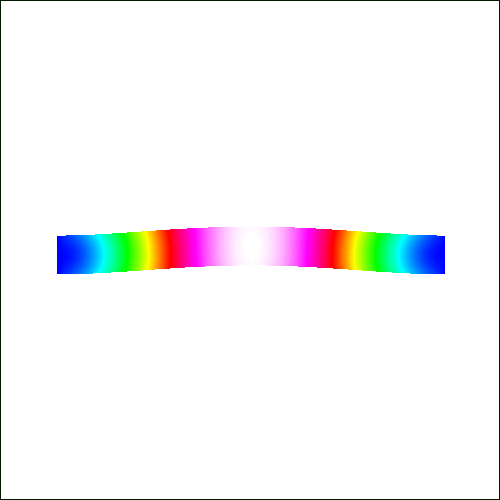
\includegraphics[width=0.4\textwidth,angle=0]{eig1}
  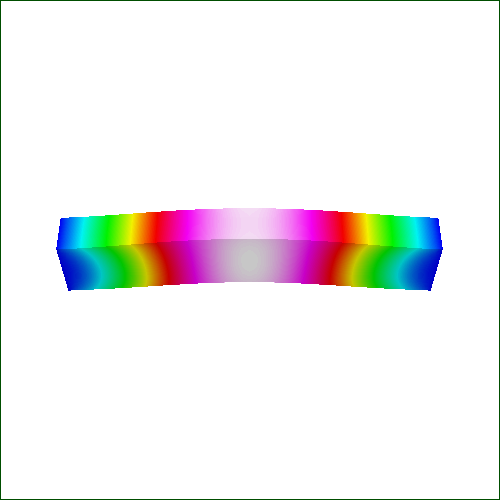
\includegraphics[width=0.4\textwidth,angle=0]{eig2}
  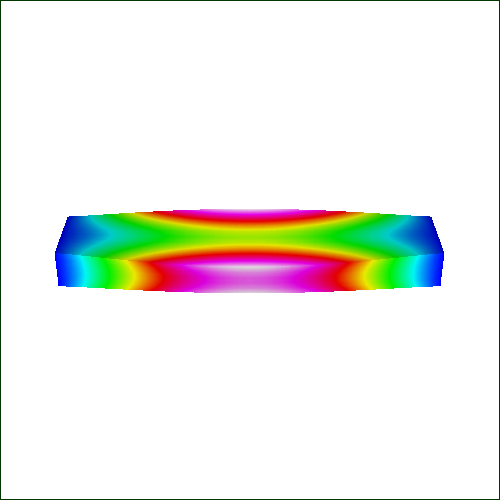
\includegraphics[width=0.4\textwidth,angle=0]{eig3}
  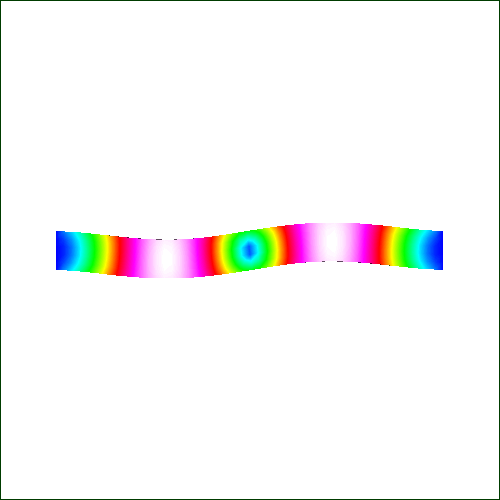
\includegraphics[width=0.4\textwidth,angle=0]{eig4}
  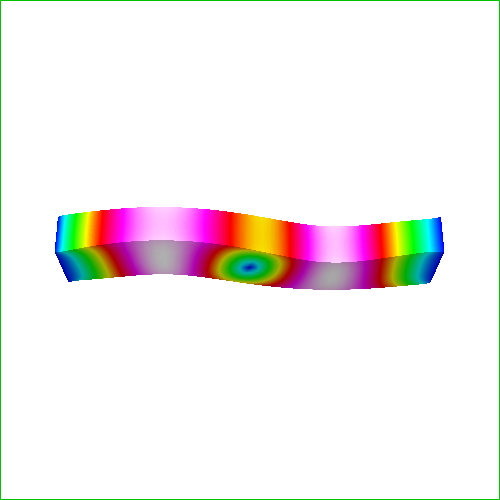
\includegraphics[width=0.4\textwidth,angle=0]{eig5}
  \caption{Eigenvectors}
  \label{fig:eig12345}
\end{center}
\end{figure}

\vfill

\graphicspath{{./}{ElasticPlateLinear/}}
\chapter{Elastic linear plate}

\modinfo{Directory}{\Idx{ElasticPlateLinear}}
\modinfo{Solvers}{\Idx{SmitcSolver}}
\modinfo{Tools}{\Idx{ElmerGrid}, editor}
\modinfo{Dimensions}{2D}

\subsection*{Case definition}

This tutorial demonstrates how to use the Smitc solver to solve
small deflections of plates.
The Smitc solver is for elastic linear plates and
uses the theory of Reissner and Mindlin.

The case under investigation is a L-shaped steel plate under pressure.
The plate is shown in figure~\ref{fig:simplePlate}
The longer sides have the length of $2\,m$ and the shorter $1\,m$. 
So the area of the plate is $3\,m^2$. The plate has a thickness of
$1\,cm$. We assume that on the plate
there is about $15300\,kg$ of sand. The sand is uniformly distributed
on the plate and the sand stays uniformly distributed even if the 
plate undergoes small deflection. The sand exerts to the plate
a pressure of $50000\,Pa$. The plate is clamped from all sides
meaning that both deflection and rotation are zero on all edges.
%
\begin{figure}[tbhp]
\begin{center}
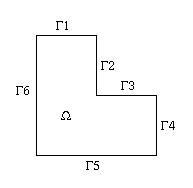
\includegraphics[width=0.4\textwidth]{simplePlate}
\end{center}
\caption{The geometry of plate and the numbering of edges.}
\label{fig:simplePlate}
\end{figure}

\subsection*{Solution Procedure}

The first thing to do is create a mesh with ElmerGrid.
The definition of mesh is in the file \texttt{simple\_plate.grd}.
The mesh is about uniform and consist of 1000 linear square elements.
The mesh is created with command
\ttbegin
ElmerGrid 1 2 simple_plate
\ttend
One thousand element should easily do the trick in this case
but if more elements is needed you can edit the file 
\texttt{simple\_plate.grd}.
More specifically the line
\ttbegin
Surface Elements = 1000
\ttend

The solver input file \texttt{simple\_plate.sif} starts with turning on 
the warnings and the definition of the proper mesh directory. 
%
\ttbegin
check keywords warn

Header
  Mesh DB "." "simple_plate"
End
\ttend
The simulation uses 2D cartesian geometry. The simulation is not
time dependent i.e. Steady State. 
There is no coupled solvers so only one iteration is needed. 
The output interval is one meaning all intervals (now there is only one
interval). Numerical results are written to file \texttt{simple\_plate.result}
and ElmerPost file is \texttt{simple\_plate.ep}.
\ttbegin
Simulation
  Coordinate System = Cartesian 2D
  Simulation Type = Steady State
  Steady State Max Iterations = 1
  Output Intervals = 1
  Output File = "simple_plate.result"
  Post File = "simple_plate.ep"
End
\ttend
There is just one body, the plate, and it uses Equation and  Body Force 1 and
is of Material 1.
\ttbegin
Body 1
  Equation = 1
  Body Force = 1
  Material = 1
End
\ttend
The equation block is now more than easy. 
It only states that we use Solver 1 to solve the equation.
\ttbegin
Equation 1
  Active Solvers(1) = 1
End
\ttend
In Body Force block we give the equations right hand side. 
It is the sands pressure and it is the same constant in every point.
\ttbegin
Body Force 1
  Pressure = 5.0e4
End
\ttend
In Material block we define the plates properties i.e. Poisson ratio,
Young's modulus and density. We also give the plates thickness and
possible pretension. Now there is no pretension.
\ttbegin
Material 1   
  Poisson ratio = 0.3
  Youngs modulus = 209e9
  Density = 7800.0

  Thickness = 1.0e-2
  Tension = 0.0
End
\ttend
Next the Solver block.
\begin{itemize}
\item First we define that we use SmitcSolver  
and give the name of the subroutine file \texttt{Smitc} and
subroutine name \texttt{SmitcSolver}. 
\item We name the variable Deflection and state that it has 3 degrees of freedom. 
First degree is the deflection and the remaining two are actually 
the components of rotation vector. 
\item We don't need eigen analysis nor is there any holes in the plate. 
\item We solve the matrix equation iteratively with stabilized biconjugate 
gradient method. We precondition the iteration with incomplete 
LU-factorization. 
\item Tolerance for the matrix system is $1\cdot10^{-8}$
and the tolerance should be achieved in less than 300 iteration.
\end{itemize}
\ttbegin
Solver 1
  Equation = "SmitcSolver"
  Procedure = "Smitc" "SmitcSolver"

  Variable = Deflection
  Variable DOFs = 3

  Eigen Analysis = False
  Hole Correction = False

  Linear System Solver = Iterative
  Linear System Iterative Method = BiCGStab
  Linear System Preconditioning = ILU2
  Linear System Convergence Tolerance = 1.0e-8
  Linear System Max Iterations = 300
End
\ttend
Finally we give the boundary conditions. The plate has 6 edges and
the edge numbering is in figure~\ref{fig:simplePlate}. All the edges are
clamped i.e. no deflection (Deflection 1) and  no rotation (Deflection 2 and 3).
\ttbegin
Boundary Condition 1
  Target Boundaries(6) = 1 2 3 4 5 6
  Deflection 1 = 0.0
  Deflection 2 = 0.0
  Deflection 3 = 0.0
End
\ttend

\subsection*{Results}

The problem is solved in few seconds and the results are viewed with
ElmerPost. It it possible to make ElmerPost to show deflection
in 3D. First we determine the number of nodes. Give commands
\ttbegin
math tmp = size(Deflection.1)
math n = tmp(1)
\ttend
to ElmerPost. Next we put the values of deflection to nodal z-values.
Deflection is rather small so the values are scaled by 50.
\ttbegin
math nodes(2,0:n-1) = 50*Deflection.1
\ttend
Result is shown in figure~\ref{fig:simplePlateDeflection}.

Deflection.2 and Deflection.3 are the x- and y-components of rotation vector.
Values are transformed to vector Rotation with commands
\ttbegin
math Rotation = 0
math Rotation(0,0:n-1) = Deflection.2
math Rotation(1,0:n-1) = Deflection.3
math Rotation(2,0:n-1) = Deflection.2*0
\ttend
The length of vector is calculated with
\ttbegin
math AbsRotation = sqrt( vdot(Rotation,Rotation) )
\ttend
%Result is shown in figure~\ref{fig:simplePlateRotation}.
Result is shown in figure~\ref{fig:simplePlateDeflection}.

It is rather cumbersome to write all the commands every time
you solve the problem. It is possible to write the commands
to file. The file, let us name it \texttt{Draw}, would be
\ttbegin
math tmp = size(Deflection.1);
math n = tmp(1);

math nodes(2,0:n-1) = 50*Deflection.1;

math Rotation=0;
math Rotation(0,0:n-1) = Deflection.2;
math Rotation(1,0:n-1) = Deflection.3;
math Rotation(2,0:n-1) = Deflection.2*0;

math AbsRotation = sqrt( vdot(Rotation,Rotation) );

display;
\ttend
The file is executed in ElmerPost with command {\tt source Draw}.
%
\begin{figure}[tbhp]
\begin{center}
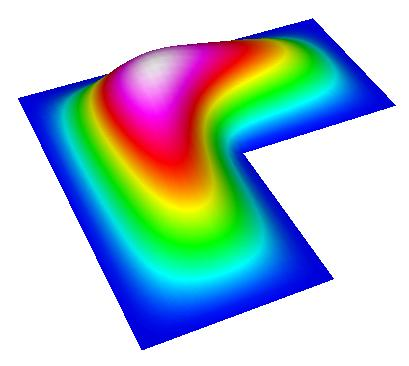
\includegraphics[width=0.48\textwidth]{simplePlateDeflection}
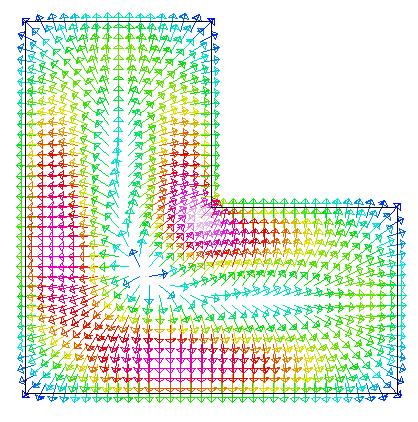
\includegraphics[width=0.48\textwidth]{simplePlateRotation}
\end{center}
\caption{The deflection of the plate and the corresponding rotation.}
\label{fig:simplePlateDeflection}
\end{figure}
%
%\begin{figure}[tbhp]
%\begin{center}
%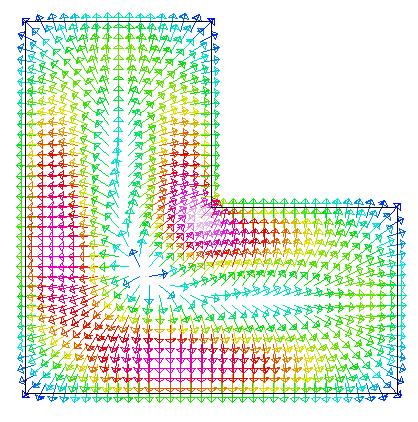
\includegraphics[width=0.5\textwidth]{simplePlateRotation}
%\end{center}
%\caption{The rotation of the plate.}
%\label{fig:simplePlateRotation}
%\end{figure}



\graphicspath{{./}{FlowStepIncompressible/}}
\chapter{Incompressible flow passing a step}
\label{tut:stepflow}

\section{Solution with linear triangles}

\modinfo{Directory}{\Idx{FlowStepIncompressible}}
\modinfo{Solvers}{\Idx{FlowSolve}}
\modinfo{Tools}{\Idx{ElmerFront}}
\modinfo{Dimensions}{2D, Steady-state}


\subsection*{Case definition}

A fluid, flowing past a step (see figure~\ref{fg:struct2}), has the density
1~kg/m$�$ and viscosity 0.01~kg/ms. The velocity of the fluid on the 
incoming boundary $\Gamma_6$ in the x-direction is 1~m/s and in 
the y-direction 0~m/s (see figure~\ref{fg:struct2}). On the outcoming boundary 
$\Gamma_4$ the velocity is 0~m/s in the y-direction and the pressure
is 0~Pa. The problem is to solve the velocity field and the pressure 
change in $\Omega$.

\begin{figure}[h]
\centering
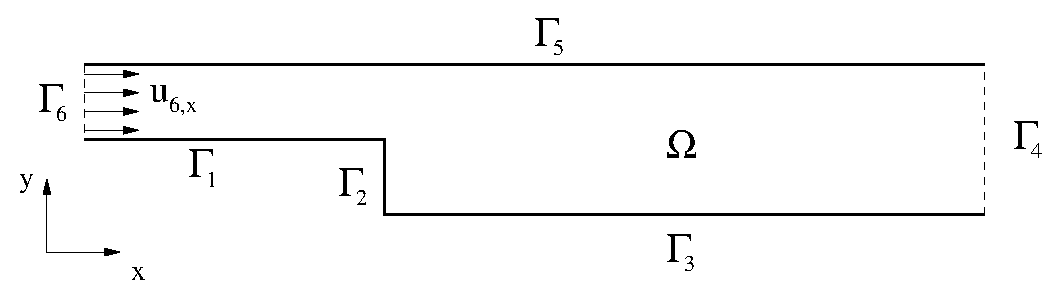
\includegraphics[width=100mm]{Body1}
\caption{Step.}\label{fg:struct2}
\end{figure}

Mathematically the problem to be solved is
\begin{equation}
\left \{
\begin{array}{rccl}
- \nabla \cdot (2 \mu \overline{\overline{\varepsilon}}) + \rho 
\vec{u} \cdot \nabla \vec{u} + \nabla p & = & 0 & \mbox{ in } \Omega \\
\nabla \cdot \vec{u} & = & 0 & \mbox{ in } \Omega \\
\end{array}
\right .
\end{equation}
with the boundary conditions
\begin{equation}
\left \{
\begin{array}{rccl}
\vec{u}_{x} & = & 1 & \mbox{ on } \Gamma_6 \\
\vec{u}_{x} & = & 0 & \mbox{ on } \Gamma_i ,\: i=1,2,3,5 \\
\vec{u}_{y} & = & 0 & \mbox{ on } \Gamma_i ,\: i=1,\ldots,6, 
\end{array}
\right .
\end{equation}
where $\mu$ is the viscosity, $\overline{\overline{\varepsilon}}$ is 
the strain tensor,  $\rho$ is the density, $\vec{u}$ is the velocity and
$p$ is the pressure. It is assumed that the density and viscosity are 
constants. 

\subsection*{Solution procedure}

\begin{itemize}
\item Start ElmerFront.
\item Open the file that contains the geometry of the step from 
the File menu. Select also the working directory for the model.
\ttbegin
File -> Open cad-file 
  File = StepFlow.egf 
  Model name = StepFlow 
  Model directory = step_tutorial
\ttend
\item Select the equations to be solved from the Problem menu. In this 
case we solve the Navier-Stokes equations.
\ttbegin
Problem -> Equations 
  Navier-Stokes 
\ttend
\item Define the material properties from the Model menu. Give the values for 
the density and the viscosity.
\ttbegin
Model -> Materials 
  Density = 1 
  Viscosity = 0.01
\ttend
\item Define boundary conditions from the Model menu. Give the values of 
the velocities at each boundary \begin{math}\Gamma_i\end{math}. Add the 
different boundary conditions to boundary condition sets and attach each 
constraint to a boundary or boundaries \begin{math}\Gamma_i\end{math} that 
the constraint concernes (see figure~\ref{fg:struct2}).
\ttbegin
Model -> Boundary conditions 
  {\it on }\begin{math}{\Gamma_6}\end{math}: Velocity-X = 1 and Velocity-Y = 0 
  {\it on }\begin{math}\Gamma_i,\: i=1,2,3,5\end{math}: Velocity-X = 0 and Velocity-Y = 0 
  {\it on }\begin{math}\Gamma_4\end{math}: Velocity-Y = 0
\ttend
\item Define mesh from the Mesh menu. First give name for 
the mesh and then define the element size. Create the mesh by pressing
``Generate mesh'' button. 
\ttbegin
Mesh -> Define mesh 
  Mesh name = Mesh1 
  Model Mesh H [m] = 0.2 
  Generate mesh
\ttend
\item Now to solve the problem select from the Run menu item Solver. This 
starts the solver. 
\ttbegin
Run -> Solver 
\ttend
\item After the solution is done, view the results by selecting from the Run
menu item Postprocessor. 
\ttbegin
Run -> Postprocessor 
\ttend
\item To save the created model, select from the File menu item Save 
model file. 
\ttbegin
File -> Save model file 
\ttend
\item To exit Elmer select from the File menu item Exit. 
\ttbegin
File -> Exit
\ttend
\end{itemize}

\subsection*{Results}

As a result the maximum pressure difference and maximum velocity is 
given (see table~\ref{tb:struct2}). One special result of interest 
is the point, on the x-axis, at which the direction of the flow changes. 
In this case its position is about 8.3 m. 
   
\begin{table}[h]
\caption{Pressure difference and velocity}
\label{tb:struct2}
\begin{center}
\begin{tabular}{lll} \hline
Elements & $\max (\Delta p)$ [Pa] & $\max |\vec{u}|$ [m/s] \\ \hline
1426  & 1.039  & 1.489 \\ \hline
\end{tabular}
\end{center}
\end{table}



\section{Solution with 2nd order rectangles}

\modinfo{Solvers}{\Idx{FlowSolve}}
\modinfo{Tools}{\Idx{ElmerGrid}, editor}
\modinfo{Dimensions}{2D, Steady-state}

\subsection*{Case definition}

In the following the flow past a step -problem is solved with
eight-noded quadrilateral elements. The mesh is done with ElmerGrid
which is a simple mesh generator that can be downloaded via the Elmer
internet pages. Here a grd file is introduced. It contains the
geometry data and parameters needed in defining the mesh of the
structure. ElmerGrid transforms this file into Elmer mesh files
(mesh.boundary, mesh.nodes, mesh.header and mesh.elements).



\subsection*{Solution procedure}

The problem might be solved using ElmerFront by reading an external
mesh into the program but here instructions for command line usage of
Elmer are given.
\begin{itemize}
\item First generate mesh with ElmerGrid with the following command.
\ttbegin 
ElmerGrid 1 2 Step.grd
\ttend

\item Make the necessary changes to the .sif file. Changes are made to
header section, boundary conditions and boundaries. The sif file is
conveniently edited using a text editor. The sections should be edited
into the following form
\ttbegin 
Header
  CHECK KEYWORDS Warn
  Mesh DB "." "Step"
End

Boundary Condition 1
  Name = "Constraint1"
  Target Boundaries(1) = 1

  Velocity 1 = 1
  Velocity 2 = 0
End

Boundary Condition 2
  Name = "Constraint2"
  Target Boundaries(1) = 3

  Velocity 1 = 0
  Velocity 2 = 0
End

Boundary Condition 3
  Name = "Constraint3"
  Target Boundaries(1) = 2

  Velocity 2 = 0
End
\ttend
\item To solve the problem run the solver by typing {\tt Solver}. 
\end{itemize}


\subsection*{Results}

In Table~\ref{tb:struct2_2} are the results of the problem solved with 
eight-noded quadrilateral (408) and three-noded triangular (303) elements.  

\begin{table}[htbp]
\centering
\begin{tabular}{l l l l} \hline
Element type  & Elements & $\max (\Delta p)$ [Pa] & $\max |\vec{u}|$ [m/s] \\ \hline
408 &  531 & 1.182  & 1.404  \\
303 & 1416 & 1.039  & 1.489  \\ \hline
\end{tabular}
\caption{Pressure difference and maximum velocity with 2nd order
rectangles and first order triangles.}\label{tb:struct2_2}
\end{table}

When the problem is solved with eight-noded quadrilateral elements the point
at which the flowing direction changes is about 8.5 m.









\graphicspath{{./}{FlowStepCompressible/}}
\chapter{Compressible flow passing a step}

\modinfo{Directory}{FlowStepCompressible}
\modinfo{Solvers}{\Idx{FlowSolve}, \Idx{HeatSolve}}
\modinfo{Tools}{\Idx{ElmerGrid}, Editor}
\modinfo{Dimensions}{2D, Steady-state}

\subsection*{Case definition}

This tutorial demonstrates how to simulate the compressible air flow passing a step. The whole step has length of 1.4 m and the height of 0.2 m and the first part of it has length of 0.4 m and the height of 0.1 m (Figure \ref{fg:step_geometry}). The needed material parameters of air are shown in Table \ref{tb:matpam}. 
The model has three sets of boundary conditions.
The air flows into the step from the inlet region and withdraws from the outlet region. The other edges of the step compose the third boundary. The flowing air is considered as an ideal gas in this case, and its density $\rho$  depends on the pressure $p$ and temperature $T$ through the equation of state
\begin{displaymath}
\rho = \frac{p}{RT},
\end{displaymath}
where $R$ is the gas constant.

\begin{figure}[h]
\centering
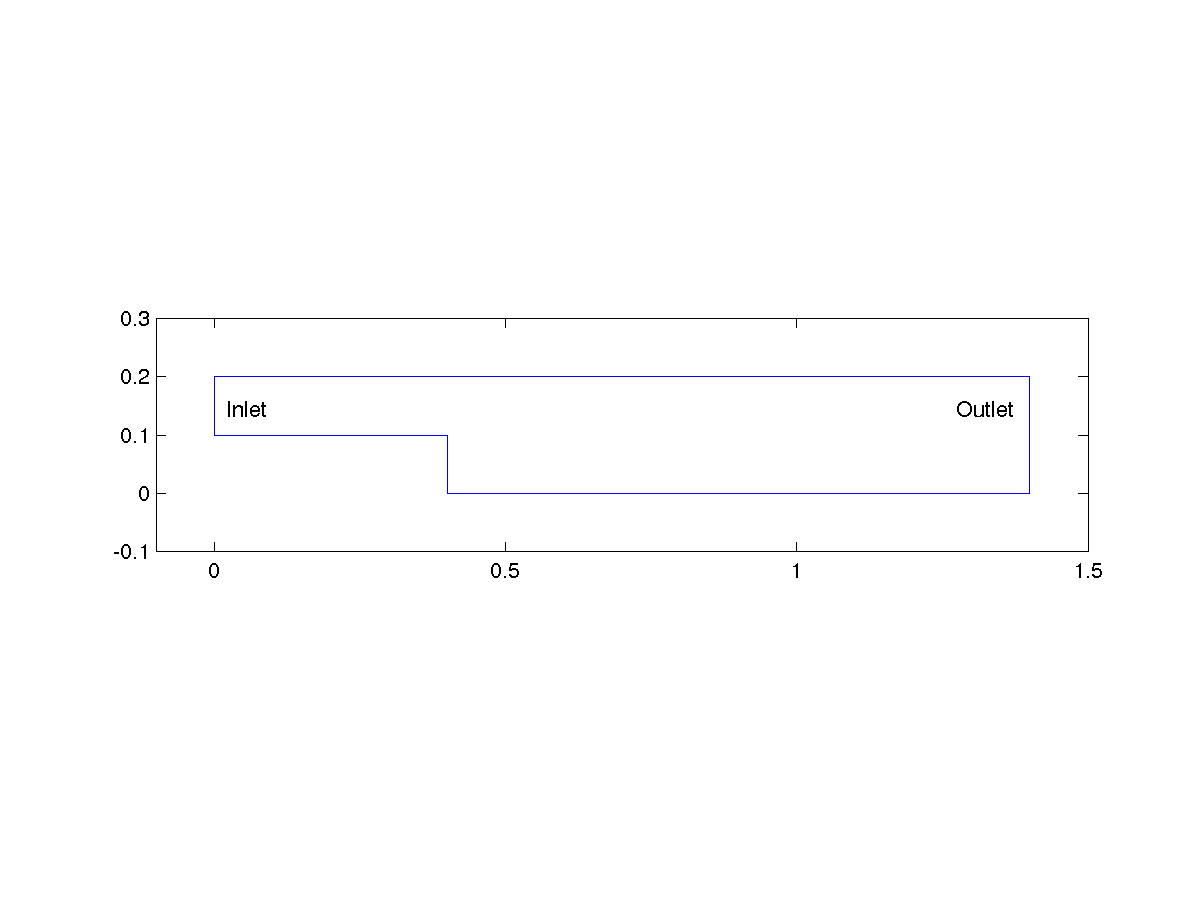
\includegraphics[height=80mm]{step_geometry.png}
\caption{Step.}\label{fg:step_geometry}
\end{figure}

\begin{table}[h]
\caption{Material parameters.}
\label{tb:matpam}
\begin{center}
\begin{tabular}{ll} \hline
parameter  & value \\ \hline
viscosity & 16.7e-6 Ns/m$^{2}$  \\
heat conductivity & 0.026 W/(m$\cdot$K) \\
heat capacity & 1.01e3 J/(kg$\cdot$K) \\
specific heat ratio & 1.4        \\
reference pressure & 1e5 Pa      \\ \hline
\end{tabular}
\end{center}
\end{table}


\subsection*{Solution procedure}

\begin{flushleft}

The mesh consists of 500 rectangular elements and it is constructed using ElmerGrid with the following command

\ttbegin
ElmerGrid 1 2 mesh.grd
\ttend

This command creates the subdirectory {\tt mesh} which contains the Elmer mesh files.

\ttbegin
Header
  Mesh DB "." "mesh"
  Include Path ""
  Results Directory ""
End
\ttend

The simulation uses 2D cartesian geometry and the problem is solved in steady state using no more than twenty steady state iterations.

\ttbegin
Simulation
  Coordinate System =  Cartesian 2D
  Coordinate Mapping(3) = 1 2 3
  Simulation Type = Steady
  Steady State Max Iterations = 20
  Solver Input File = "compress_step.sif"
  Post File = "compress_step.ep"
  Output File = "compress_step.dat"
End
\ttend

The solvers are coupled and therefore the convection is computed. 

\ttbegin
Equation 1
  Navier-Stokes = True
  Heat Equation = True
  Convection = "Computed"
End
\ttend

Due to the simplicity of the model only one body is needed.

\ttbegin
Body 1
  Equation = 1
  Material = 1
  Initial Condition = 1
End
\ttend

Our intention is to model compressible flow and that is why we have to set the value ''Perfect Gas'' for the keyword {\tt Compressibility Model}. Furthermore, because perfect gas model has been chosen the settings {\tt Reference Pressure} and {\tt Specific Heat Ratio} must also be given. The Navier-Stokes equation also needs the value of viscosity and the heat equation needs the values of heat capacity and heat conductivity.

\ttbegin
Material 1
  Compressibility Model = String "Perfect Gas"
  Reference Pressure = 1e5
  Specific Heat Ratio = 1.4
  Viscosity = 16.7e-6
  Heat Conductivity = 0.026
  Heat Capacity = 1.01e3
End
\ttend

For the initial value of temperature we have chosen 300 K.

\ttbegin
Initial Condition 1
  Temperature = 300
End
\ttend

The Navier-Stokes equation is solved first. Here we give the linear system solver and convergence criterions for linear, nonlinear and steady state solution of the Navier-stokes equation. Note that we are solving for the compressible Navier-stokes equation and that is why a bubble function formulation is used for stabilization of the equation.


\ttbegin
Solver 1
  Equation = "Navier-Stokes"
  Linear System Solver = "Iterative"
  Linear System Iterative Method = "BiCGStab"
  Linear System Max Iterations = 500
  Linear System Convergence Tolerance = 1.0e-08
  Linear System Abort Not Converged = True
  Linear System Preconditioning = "ILU2"
  Linear System Residual Output = 1
  Steady State Convergence Tolerance = 1.0e-05
  Bubbles = Logical True
  Nonlinear System Convergence Tolerance = 1.0e-05
  Nonlinear System Max Iterations = 1
  Nonlinear System Newton After Iterations = 3
  Nonlinear System Newton After Tolerance = 1.0e-02
  Nonlinear System Relaxation Factor = 1
End
\ttend

The corresponding parameters for the solver of the heat equation are defined in the following solver section.

\ttbegin
Solver 2
  Equation = "Heat Equation"
  Variable = "Temperature"
  Linear System Solver = "Iterative"
  Linear System Iterative Method = "BiCGStab"
  Linear System Max Iterations = 350
  Linear System Convergence Tolerance = 1.0e-08
  Linear System Preconditioning = "ILU0"
  Linear System Residual Output = 1
  Steady State Convergence Tolerance = 1.0e-05
  Bubbles = Logical True
  Nonlinear System Convergence Tolerance = 1.0e-05
  Nonlinear System Max Iterations = 1
  Nonlinear System Newton After Iterations = 3
  Nonlinear System Newton After Tolerance = 1.0e-02
  Nonlinear System Relaxation Factor = 1
End
\ttend

Finally, the boundary conditions are specified. There are three sets of boundary conditions, so three {\tt Boundary Condition} sections are needed. The first one is used to prescribe the boundary conditions in the inlet region. Note that we have defined the x-velocity and temperature as a variable of y-coordinate. 
This is done by setting different values for the x-velocity and temperature 
(the numerical values of the second column between the words {\tt Real} and {\tt End})
in the different y-points
(the numerical values of the first column between words {\tt Real} and {\tt End})
of the inlet region.
This kind of procedure prevents occuring singularities in the corner points of the inlet region. In addition, this kind of definition is more realistic than a condition, inwhich the values of the x-velocity and temperature remain the same in the whole inlet region. 

\ttbegin
Boundary Condition 1
  Target Boundaries = 1
  Velocity 1 = Variable Coordinate 2
    Real 
      0.1    0
      0.15   0.02
      0.2    0
    End

  Velocity 2 = 0
  Temperature = Variable Coordinate 2
    Real 
      0.1    300
      0.15   350
      0.2    300
    End
End
\ttend

After the rest boundary conditions have been defined the problem is ready to solve.

\ttbegin
Boundary Condition 2
  Target Boundaries = 2
  Velocity 2 = 0
End

Boundary Condition 3
  Target Boundaries = 3
  Velocity 1 = 0
  Velocity 2 = 0
  Temperature = 300
End
\ttend

\subsection*{Results}

Figure \ref{fg:comp_step_temp} presents the temperature distribution of the step in steady state. The maximum and minimum values of x- and y-velocities are also given as a result and they are shown in Table \ref{tb:velocities}.

\begin{figure}[h]
\centering
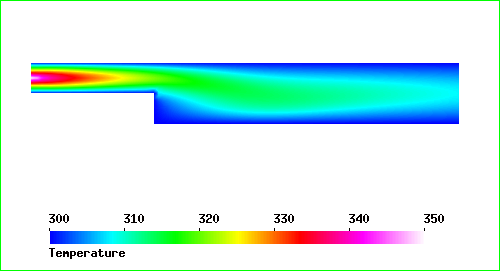
\includegraphics[height=80mm]{comp_step_temp.png}
\caption{Step.}\label{fg:comp_step_temp}
\end{figure}

\begin{table}[h]
\caption{Computed velocities.}
\label{tb:velocities}
\begin{center}
\begin{tabular}{ll} \hline
velocity  & value \\ \hline
min x-velocity & -0.0014 m/s\\
min y-velocity & -0.0016 m/s        \\
max y-velocity & 0.0008 m/s      \\ \hline
\end{tabular}
\end{center}
\end{table}

\end{flushleft}

\vfill

\graphicspath{{./}{Electrostatics/}}
\chapter{Electrostatics}

\modinfo{Directory}{\Idx{Electrostatics}}
\modinfo{Solvers}{\Idx{StatElecSolve}, \Idx{ElectricForce}}
\modinfo{Tools}{\Idx{ElmerGrid}, editor}
\modinfo{Dimensions}{3D, Steady-state}

\subsection*{Case definition}

This case presents solving the Poisson equation for electric potential
and calculating appropriate derived quantities, such as
\Idx{capacitance}, based on the result. The geometry studied is a
symmetric quadrant of a plane capacitor having a rectangular hole in
another plate. A setting of this kind can be used to study the effects
of geometrical features on the capacitance and on the electrostatic
force, which both are meaningful quantities for coupled
simulations in {\em e.g.}  microsystems.


\subsection*{Solution procedure}

The mesh is constructed using ElmerGrid with the following command
\ttbegin
ElmerGrid 1 2 elmesh.grd
\ttend
The mesh is extended above the hole to avoid undesired boundary
effects. The geometry is presented in the Figure~\ref{geo_elstat}

\begin{figure}[hbt]
  \centerline{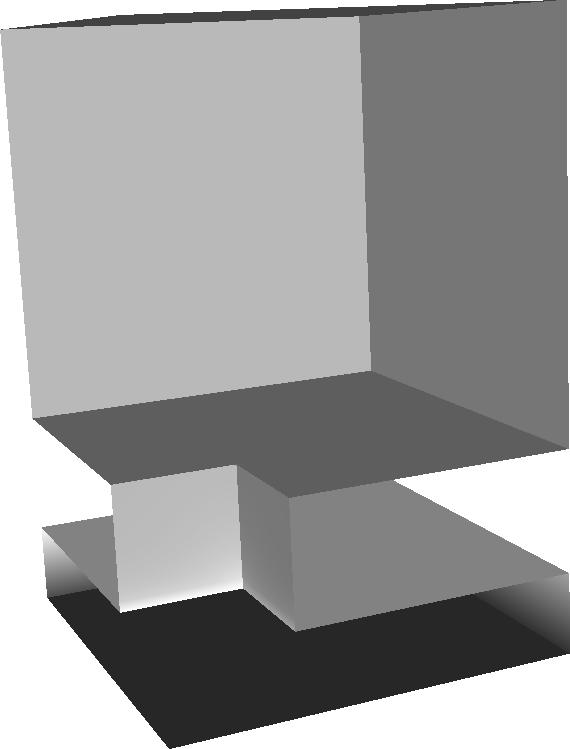
\includegraphics[width=0.32\textwidth]{geo_elstat}}
  \caption{The geometry of problem.} 
  \label{geo_elstat}
\end{figure}

The simulation problem includes a single body, and thus one material
and one equation set, as well as three solvers. The solvers are used
to compute the electric potential and related quantities, to calculate
the electric force, and to save relevant data into a file. This
tutorial is defined in Elmer \Idx{MEMS} units. The sif-file is presented
below.

\ttbegin
Check Keywords Warn

Header
  Mesh DB "." "elmesh"
End
\ttend

Only a single steady state iteration is needed, since the Poisson
equation is linear.
\ttbegin
Simulation
  Coordinate System = Cartesian 3D
  Simulation Type = Steady State
  Steady State Max Iterations = 1
  Output File = "elstatics.result"
  Post File = "elstatics.ep"
End
\ttend

The permittivity of vacuum has to be defined in the Constants section.
\ttbegin
Constants
  Permittivity Of Vacuum = 8.8542e-12
End

Body 1
  Equation = 1
  Material = 1
End
\ttend

Electric energy density is added into the results in Equation
section. This allows energy density to be visualised in
ElmerPost. Note also, that calculating electric flux (or the electric
displacement field) is disabled in the Solver~1 block. Further, the
potential difference used in calculating the capacitance of the system
has to be defined in this section. This should be the same as the
boundary conditions define for the capacitance calculation to be
sensible.
\ttbegin
Equation 1
  Active Solvers(2) = 1 2
  Calculate Electric Energy = True  ! (default False)
End

Solver 1
  Equation = Stat Elec Solver
  Variable = Potential
  Variable DOFs = 1
  Procedure = "StatElecSolve" "StatElecSolver"
  Calculate Electric Field = True  ! (default True)
  Calculate Electric Flux = False  ! (default True)
  Potential Difference = 1.0e6
  Linear System Solver = Iterative
  Linear System Iterative Method = BiCGStab
  Linear System Max Iterations = 200
  Linear System Convergence Tolerance = 1.0e-07
  Linear System Preconditioning = ILU1
  Linear System ILUT Tolerance = 1.0e-03
  Nonlinear System Max Iterations = 1
  Nonlinear System Convergence Tolerance = 1.0e-4
  Nonlinear System Newton After Tolerance = 1.0e-3
  Nonlinear System Newton After Iterations = 10
  Nonlinear System Relaxation Factor = 1
  Steady State Convergence Tolerance = 1.0e-4
End
\ttend

The static electric force solver does not need a lot of
information:
\ttbegin
Solver 2
  Equation = Electric Force
  Procedure = "ElectricForce" "StatElecForce"
End
\ttend

Finally, some data is saved in file scalars.dat in working directory.
\ttbegin
Solver 3
  Exec Solver = After All
  Equation = SaveScalars
  Procedure = "\Idx{SaveData}" "SaveScalars"
  Filename = "scalars.dat"
End
\ttend

Only the relative permittivity of the material has to be defined.
\ttbegin
Material 1
  Relative Permittivity = 1
End
\ttend

The boundary conditions include the values of electric potential
(voltage) and indication on which boundary the electric force should
be calculated. On all the other boundaries a natural boundary
condition is used, basically stating that the electric flux through
these boundaries is zero.
\ttbegin
Boundary Condition 1
  Target Boundaries = 4
  Potential = 0.0
  Calculate Electric Force = True
End

Boundary Condition 2
  Target Boundaries = 3
  Potential = 1.0e6
End
\ttend


\subsection*{Results}

The results obtained for capacitance and electric force are compared
to those of a complete plane capacitor. For a plane capacitor, the
capacitance is
\begin{equation}
C=\varepsilon_r\varepsilon_0\frac{A}{d},
\end{equation}
and the electrostatic force is
\begin{equation}
F_e = \frac{1}{2}\varepsilon_r\varepsilon_0\frac{A}{d^2}\Phi^2,
\end{equation}
where $\varepsilon_r$ is the relative permittivity, $\varepsilon_0$
is the permittivity of vacuum, $A$ is the area of a capacitor plate,
$d$ is the separation of the capacitor plates, and $\Phi$ is the
potential difference between the plates.

The results of the simulation as well as the comparison to the
complete plane capacitor values are shown in Table~\ref{tab_elstatics}
(in Elmer MEMS units). Note that the fringe fields on capacitor edges
are not calculated. This would require much larger mesh extending
outside the capacitor boundaries.

\begin{table}[htb]
\caption{Comparison of numerical results to analytic values}
\label{tab_elstatics}
\begin{center}
\begin{tabular}{lccc} \hline
            & simulation & analytic & ratio \\ \hline
Capacitance & \ \ $2.1361\cdot 10^{-10}$\ \  & 
              \ \ $2.2136\cdot 10^{-10}$\ \  & 0.965 \\
Electric Force & $1.0406\cdot 10^2$ & 
                 $1.1068\cdot 10^2$ & 0.940 \\ \hline
\end{tabular}
\end{center}
\end{table}

Finally, a picture of the results is presented. The
Figure~\ref{res_elstat} shows the isosurfaces of the electric
potential with the color marking the strength of the electric
field. From the picture it is clearly seen that the electric field is
constant between the plates except for the proximity of the hole which
causes weakening of the field magnitude. There are also strong
electric fields at the edges of the hole.


\begin{figure}[hbt]
  \centerline{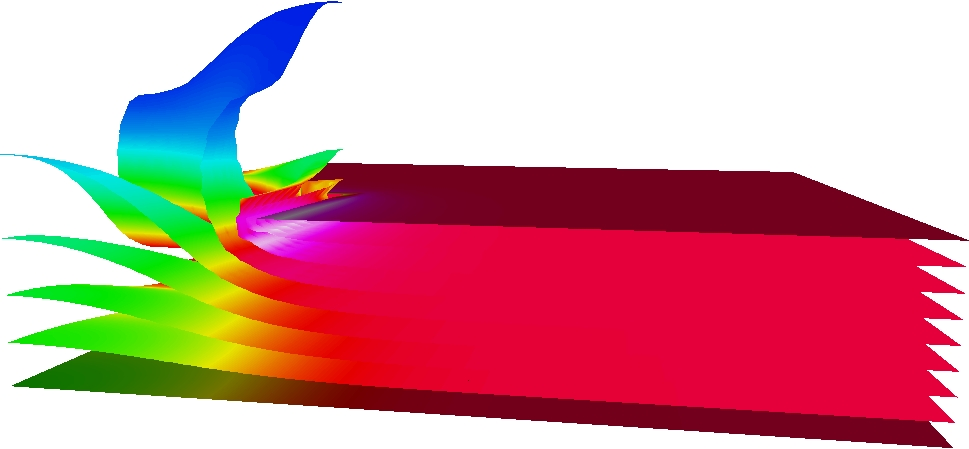
\includegraphics[width=0.8\textwidth]{res_elstat}}
  \caption{Isosurfaces of the potential coloured with electric field
  magnitude.} 
  \label{res_elstat}
\end{figure}



\vfill
\mbox{}



\graphicspath{{./}{AcousticWaves/}}
\chapter{Lossless \Idx{acoustic waves}}

\modinfo{Directory}{\Idx{AcousticWaves}}
\modinfo{Solvers}{\Idx{HelmholtzSolve}} 
\modinfo{Tools}{\Idx{ElmerFront}} 
\modinfo{Dimensions}{2D, Harmonic}


\subsection*{Introduction}

Elmer provides two alternative ways of conducting acoustic analyses in the
frequency domain. Firstly, one may simply use the Helmholtz equation which 
is based on the assumption of lossless flow, i.e.\ the effects of viscosity 
and heat conduction are assumed to be negligible. More refined analyses where 
these effects are taken into account may be carried out by using the specific 
solver for the set of time-harmonic dissipative acoustic equations. 
The aim of this tutorial is to demonstrate the usage of the solver
for the basic Helmholtz equation, which is frequently taken as the starting
point in acoustic analyses. 

\subsection*{Case description}

In this problem the fluctuations of the pressure in an air-filled
cavity shown in Figure~\ref{cavity.fig} are considered. The cavity is 
connected with the surrounding air by an open narrow pipe. The pressure 
fluctuations are generated by a vibrating membrane on the boundary $\Gamma_S$ 
with the frequency of the motion being $f=100$ Hz. 
The remaining parts of the boundary are assumed to be rigid walls. 
In addition, the effects of gravity are assumed to be negligible.

\begin{figure}
\setlength{\unitlength}{1mm}
\begin{center}
\begin{picture}(60,50)(0,-10)
\put(0,0){\line(1,0){50}}
\put(0,0){\line(0,1){30}}
\put(0,30){\line(1,0){21}}
\put(29,30){\line(1,0){21}}
\put(29,30){\line(0,1){10}}
\put(21,30){\line(0,1){10}}
\put(21,40){\line(1,0){8}}
\put(50,0){\line(0,1){30}}
\put(25,-1){\line(0,1){2}}
\put(40,-1){\line(0,1){2}}
\put(31,2){$\Gamma_S$}
\put(23,42){$\Gamma_0$}
\put(55,15){\vector(0,1){15}}
\put(55,15){\vector(0,-1){15}}
\put(55,35){\vector(0,1){5}}
\put(55,35){\vector(0,-1){5}}
\put(15,-5){\vector(-1,0){15}}
\put(15,-5){\vector(1,0){10}}
\put(33,-5){\vector(-1,0){8}}
\put(33,-5){\vector(1,0){7}}
\put(45,-5){\vector(-1,0){5}}
\put(45,-5){\vector(1,0){5}}
\put(15,22){\vector(-1,0){15}}
\put(15,22){\vector(1,0){6}}
\put(25,22){\vector(-1,0){4}}
\put(25,22){\vector(1,0){4}}
\put(10,-4){0.25}
\put(30,-4){0.15}
\put(43,-4){0.1}
\put(57,14){0.3}
\put(57,34){0.1}
\put(10,23){0.3}
\put(22,23){0.08}
\end{picture}
\end{center}
\caption{The geometry of the cavity.}
\label{cavity.fig}
\end{figure}

Suitable boundary conditions in terms of the pressure must be given. 
On the rigid walls the pressure flux is prescribed to vanish which 
corresponds to the assumption that there is no velocity in the direction 
normal to the boundary. At the open end $\Gamma_0$ the impedance boundary 
condition suitable for forward traveling plane waves is given by setting 
$Z=-c$ with $c$ being the sound speed. We assume that $c=343$ (m/s). 
Finally, the wave source is given by defining a non-vanishing pressure
flux on the corresponding part of the boundary. We take simply 
$\nabla P \cdot \vec n = 1$ where $P$ is the (complex)
amplitude of the pressure and $\vec n$ is the outward unit normal to the
boundary. 


\subsection*{Solution procedure}

\begin{itemize}

\item Before starting Elmer copy the geometry file ({\tt domain.egf}) to the 
working directory and then launch Elmer Front by giving the command
\ttbegin
ElmerFront
\ttend 

\item Open the geometry file by choosing Open Cad-file in the  
File menu. To enable browsing with the mouse click the button on the 
right-hand side of the field where the file name may be written. Here
the correct Cad file type is Elmer. Give also the model name (for example
{\tt helmholtz}) and write the path of the working directory in the
Model directory field.  

\item Select the equation to be solved by selecting Equations in
the Problem menu. Choose the Helmholtz equation and press 
{\tt Add} button. 

\item Define the angular frequency for the simulation by selecting 
Simulation parameters in the Problem menu. Enter the value
628.3 to the field and accept the value by clicking {\tt OK} button.

\item Define the sound speed for the medium by selecting 
Materials in the Model menu. Enter the value
343 for the sound speed and press {\tt Add} button.

\item Prescribe the boundary conditions by selecting 
Boundary conditions in the Model menu. Select (with the mouse)
Boundary1 and give the value for the boundary flux: 
\ttbegin
Wave flux Re = 1
Wave flux Re = 0
\ttend 
Finally, press {\tt Add} button. Then proceed to give 
the other boundary conditions in a similar manner (the value for the 
pressure is prescribed).

\item Create a finite element mesh  by selecting 
Define mesh in the Mesh menu. To begin with give a name for the mesh.
Define the number of element
edges on each boundary and then create the mesh by pressing
{\tt Generate Mesh} button.   

\item The problem may now be solved by selecting Solver in the Run menu.

\item After the solution is done, view the results by selecting the
Postprocessor from the Run menu.
\ttbegin
Run -> Postprocessor
\ttend
\item To save the created model, select Save model file from the File menu.
\ttbegin
File -> Save model file
\ttend
\end{itemize}


   

\subsection*{Results}

Using a mesh consisting of 3900 (quadratic) elements with 7601 nodes
the difference of the maximum and the minimum value of the pressure 
is found to be $\Delta p \approx 0.205$


   
























\part{Coupled Problems}

\graphicspath{{./}{RayleighBenard/}}
\chapter{Transient flow and heat equations -- the Rayleigh-Benard instability}

\modinfo{Directory}{RayleighBenardGUI}
\modinfo{Solvers}{\Idx{HeatSolve}, \Idx{FlowSolve}}
\modinfo{Tools}{\Idx{ElmerGUI}}
\modinfo{Dimensions}{2D, Transient}

\subsection*{Case definition}

%\begin{flushleft}
This tutorial is about simulating the developing of the
Rayleigh-Benard instability in a rectangular domain  (Figure
\ref{fg:rb_geometry}) of dimensions 0.01 m height and 0.06 m
length. The simulation is performed with water and the material
parameters of water required by the Elmer model are presented in Table \ref{tb:matpar}. The
temperature difference between the upper and lower boundary is set to
0.5 so that lower one has the temperature of  283.5 K and the upper
one has the temperature of 283 K.


The density of water is inversely proportional to its
temperature. Thus, heated water starts to flow upwards, and colder
downwards due to gravity.  In this case we assume that the
\Idx{Boussinesq} approximation is valid for thermal incompressible
fluid flow. In other words, the density of the term $\rho$$\vec{f}$ in
the incompressible Navier-Stokes equation can be redefined by the
Boussinesq approximation
\begin{displaymath}
\rho = {\rho}_0(1-\beta(T-{T}_0))
\end{displaymath}
where $\beta$ is the heat expansion coefficient and the subscript 0 refers to a reference sate.


\begin{figure}[h]
\centering
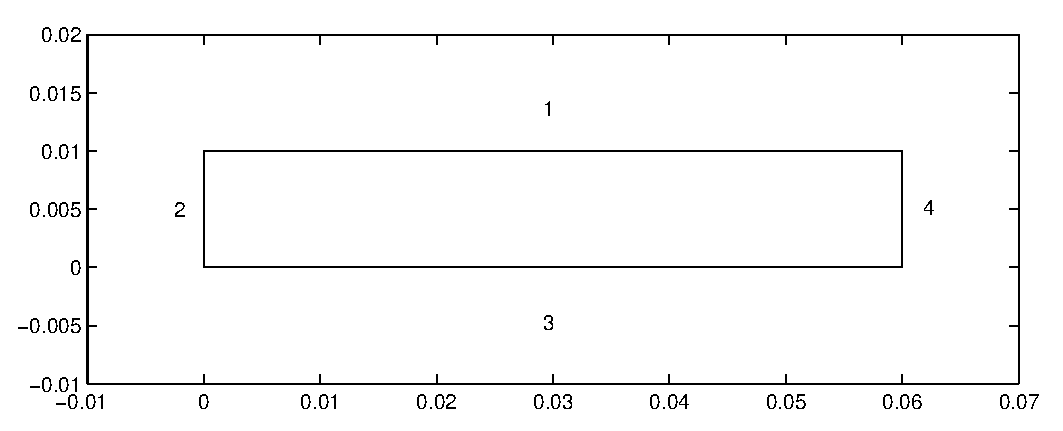
\includegraphics[width=150 mm, height=55 mm]{rb_geometry}
\caption{Domain.}\label{fg:rb_geometry}
\end{figure}  


\begin{table}[h]
\caption{Material parameters.}
\label{tb:matpar}
\begin{center}
\begin{tabular}{ll} \hline
parameter  & value \\ \hline
density & 1000 kg/m$^{3}$ \\
viscosity & 1040e-6 Ns/m$^{2}$ \\
heat capacity & 4190 J/(kg$\cdot$K) \\
heat conductivity & 0.6 W/(m$\cdot$K)       \\
heat expansion coefficient & 1.8e-4 K$^{-1}$      \\ 
reference temperature & 283 K       \\ \hline
\end{tabular}
\end{center}
\end{table}


\subsection*{Solution procedure}

The mesh is given in ElmerGrid format in file \texttt{box.grd}, load this file.
\ttbegin
File 
  Open -> box.grd
\ttend
You should obtain your mesh and may check that it consists of 3036 bilinear elements.

There is a possibility to divide and unify edges to simplify the case definition in the future.
\ttbegin
Choose (left wall + right wall (Ctrl down)) -> unify edge
\ttend

After we have the mesh we start to go through the Model menu from the top to bottom. 
In the Setup we choose things related to the whole simulation such as file names, 
time stepping, constants etc.
The simulation is carried out in 2-dimensional cartesian
coordinates. 2nd order bdf time-stepping method is selected with 200 steps
and with step size of two seconds.
\ttbegin
Model
  Setup 
    Simulation Type = Transient
    Steady state max. iter = 20
    Time Stepping Method = bdf
    BDF Order = 2
    Time Step Intervals = 200
    Time Step Sizes = 2.0
    Gravity = ...
\ttend
In the equation section we choose the relevant equations and paremeters related to their solution. 
In this case we'll have one set of equations (named ``Natural Convection'') which consists of the heat equation
and of the Navier-Stokes equation.

When defining Equations and Materials it is possible to assign the to bodies immediately, or to use mouse
selection to assign them later. In this case we have just one body and therefore its easier to assign 
the Equation and Material to it directly.
It is important to select the 
convection to be computed since that couples the velocity field to the heat equation.

The system may include nonlinear iterations of each equation and steady state iterations 
to obtain convergence of the coupled system. It is often a good idea to keep the number of 
nonlinear iterations in a coupled case low. Here we select just one nonlinear iteration
for both equations.
For the linear system solvers we are happy to use the defaults. One may however, try out different
preconditioners (ILU1,\ldots) or direct Umfpack solver, for example.
\ttbegin
Model
  Equation
    Name = Natural Convection
    Apply to Bodies = 1
    Heat Equation
      Active = on
      Convection = Computed
      Edit Solver Setting
        Nonlinear System
          Max. iteations = 1
    Navier-Stokes 
      Active = on
      Edit Solver Setting
        Nonlinear System
          Max. iteations = 1
\ttend        
The Material section includes all the material parameters.
They are divided to generic parameters which are direct properties of the material
without making any assumptions on the physical model, such as the mass. Other properties assume
a physical law, such as conductivities and viscosity.      
\ttbegin
Model
  Material
    Name = Fluid
    Apply to Bodies = 1 
    General    
      Density = 1000
      Heat Capacity = 4190
      Reference Temperature = 283
      Heat expansion Coeff. = 1.8e.4
    Heat Equation
      Heat Conductity = 0.6
    Navier-Stokes
      Viscosity = 1.04e-3
\ttend

A Body Force represents the right-hand-side of a equation. It is generally 
not a required field for a body. In this case, however, we apply the bouyancy resulting from
heat expansion as a body force to the Navier-Stokes equation.
\ttbegin
Model
  Body Force
    Name = Boyancy
    Apply to Bodies = 1
    Navier Stokes
      Boussinesq = on
\ttend    

Initial conditions should be given to transient cases. In this case we choose a constant Temperature field
and a small initial velocity. 
\ttbegin
Model
  Initial Condition 
    Name = Initial Guess
    Heat Equation
      Temperature = 283
    Navier-Stokes
      Velocity 1 = 1.0e-9
      Velocity 2 = 0.0
\ttend

Only one boundary condition may be applied to each boundary and therefore all the 
different physical BCs for a boundary should be grouped together. In this case the
Temperature and Velocity. The side walls are assumed to be adiabatic.
\ttbegin
Model
  BoundaryCondition
    Name = Bottom
    Heat Equation
      Tempateture = 283.5
    Navier-Stokes 
      Velocity 1 = 0.0
      Velocity 2 = 0.0
 
    Name = Top
    Heat Equation
      Tempateture = 283
    Navier-Stokes 
      Velocity 1 = 0.0
      Velocity 2 = 0.0
 
    Name = Sides
    Navier-Stokes 
      Velocity 1 = 0.0
      Velocity 2 = 0.0
\ttend   

The boundary conditions may also be set in the Boundary condition menu, or 
by clicking with the mouse. Here we use the latter approach as that spares us of the 
need to know the indexes of each boundary.
\ttbegin
Model
  Set boundary properties
    Choose Bottom -> set boundary condition Bottom
    Choose Top -> set boundary condition Top
    Choose Sides -> set boundary condition Sides
\ttend

After the case have been set-up we may check that all edges and surfaces have been assigned 
boundary condition, or an equation and material parameters.
\ttbegin
View
  Select defined edges 
  Select defined surfaces
\ttend 
If everything is set we may continue, otherwise one should go back to check what data is missing.
\ttbegin
View
  Reset model view
\ttend

For the execution 
ElmerSolver needs the mesh files and the command file. We have know basically defined
all the information for ElmerGUI to write the command file. After writing it we may also visually 
inspect the command file.
\ttbegin
Sif 
  Generate
  Edit -> look how your command file came out  
\ttend

Before we can execute the solver we should save the files in a directory. Both the command file and
the mesh file will be saved simultaneously to the destination directory.
\ttbegin
File 
  Save As
\ttend

After we have succefully saved the files we may start the solver
\ttbegin
Run
  Run solver
\ttend
A convergence view automatically pops up showing relative changes of each iteration.
When there are some results to view we may start the postprocessor also
\ttbegin
Run
  Run postprocessor
\ttend


\subsection*{Results}

Due to the number of the time-steps the simulation may take around ten minutes.
You may inspect the results with ElmerPost as the time-steps are computed, or
wait until all timesteps have been computed. 
When opening the result file using ElmerGUI ElmerPost only opens the first time-step.
Therefore it is important to reopen the file and load the time-steps of interest.
Pressing the button $\bf{All}$ selects all the calculated time steps.
A video of the results can be viewed by selecting the option $\bf{Timestep}$ 
$\bf{Control}$ and pressing the button $\bf{Loop}$ under the $\bf{Edit}$ menu.

In Figures \ref{fg:rb_temp} and \ref{fg:rb_vel} the obtained temperature 
distribution and the velocity vectors are presented. 
The maximum velocity in the system should be about 0.4 mm/s. 

\begin{figure}[h]
\centering
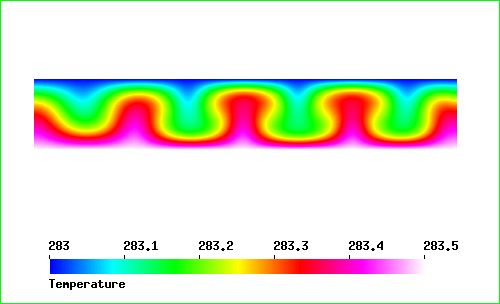
\includegraphics[width=150 mm, height=50 mm]{rb_temp}
\caption{Temperature distribution at 260 s.}\label{fg:rb_temp}
\end{figure} 

\begin{figure}[h]
\centering
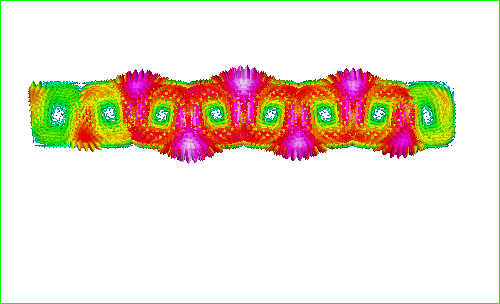
\includegraphics[width=150 mm, height=70 mm]{rb_vel}
\caption{Velocity vectors at 260 s.}\label{fg:rb_vel}
\end{figure} 







% this has changed!
%\graphicspath{{./}{CapacitanceMatrix/}}
%\chapter{Computation of a capacitance matrix}


\modinfo{Directory}{CapacitanceMatrix}
\modinfo{Solvers}{\Idx{StatElecSolve}}
\modinfo{Tools}{\Idx{ElmerGrid}, Editor}
\modinfo{Dimensions}{2D, Steady-state}

\subsection*{Case definition}

\begin{flushleft}

In Elmer, a \Idx{capacitance matrix} is possible to solve with an algorithm where a unity potential is permutated through 
all bodies and the resulting charges are registered. 

In this case the capacitancies is solved between four different bodies (Figure \ref{fg:4holegeometry}). We have assumed that the model is manufactured from glass of dimensions 5 m height and length. Due to symmetry of the model each body has the height and length of 1 m. To solve the problem we only need to know the relative permittivity of glass (Table \ref{tb:glasspar}).

\begin{figure}[h]
\centering
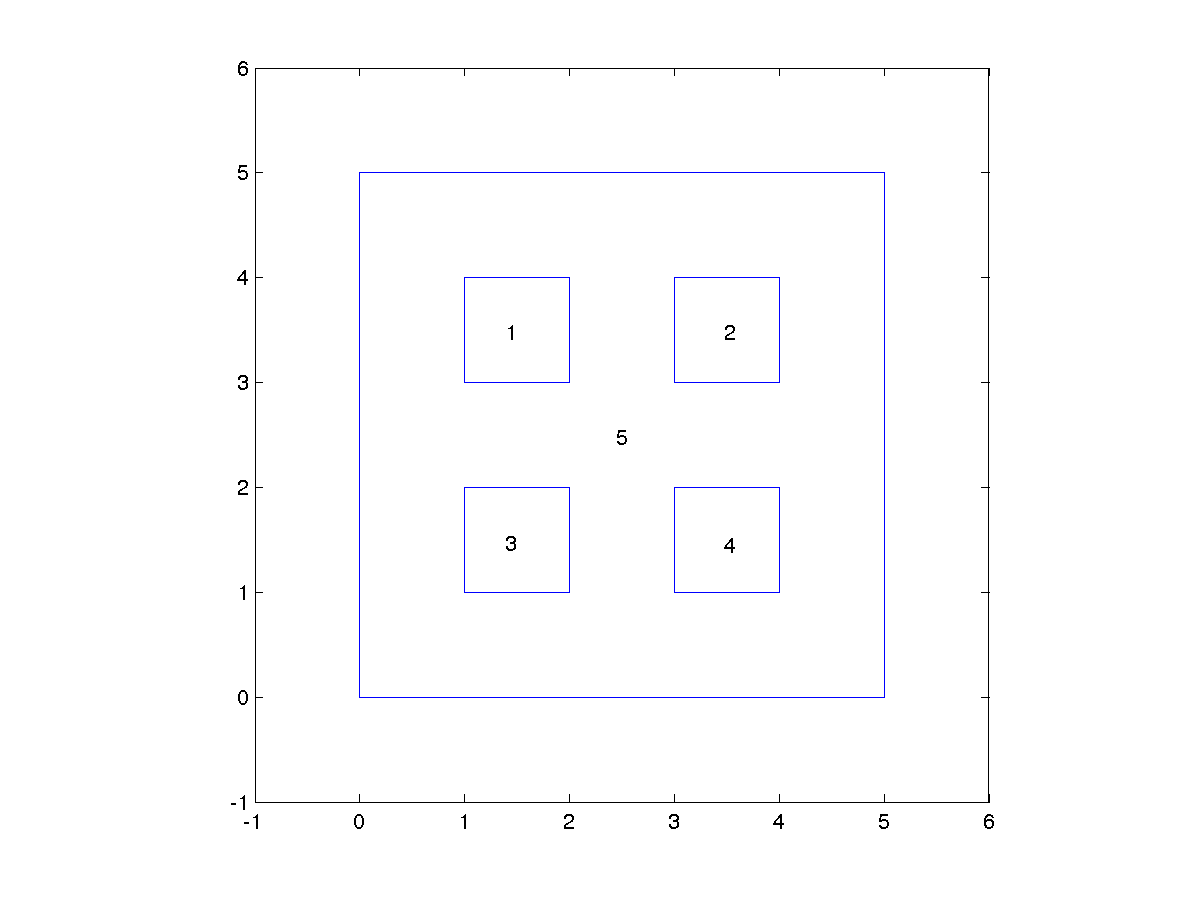
\includegraphics[height=80mm]{4holegeometry}
\caption{Geometry of the model.}\label{fg:4holegeometry}
\end{figure}


\begin{table}[h]
\caption{Material parameters.}
\label{tb:glasspar}
\begin{center}
\begin{tabular}{ll} \hline
parameter  & value \\ \hline
relative permittivity & 7      \\ \hline
\end{tabular}
\end{center}
\end{table} 


\end{flushleft}

\subsection*{Solution procedure}

\begin{flushleft}
Let us next introduce the solution procedure of the problem.
The computation mesh has been created with Gambit software and it consists of 15941 elements. The mesh can be convert into Elmer format with the command

\ttbegin
ElmerGrid 7 2 mesh.FDNEUT
\ttend

This command creates the directory {\tt mesh} which contains the mesh files. 

\ttbegin
Header
  Mesh DB "." "mesh"
End
\ttend

The simulation of the problem is carried out in a 2D cartesian geometry.
The different permutation are computed within the nonlinear iterations of the solver and therefore only one
steady state iteration is needed.

\ttbegin
Simulation
  Coordinate System = "Cartesian 2D"
  Simulation Type = "Steady"
  Output Intervals(1) = 1 
  Steady State Max Iterations = 1
  Output File = File "4_holes.result"
  Post File =   File "4_holes.ep"
End
\ttend

In the solver section the keyword {\tt Calculate Capacitance Matrix} must be set to {\tt True}. 
We also have to define the number of the bodies in our system. 
The calculated matrix is saved to file cmatrix.dat.

\ttbegin
Solver 1
  Equation = "Stat Elec Solver"
  Procedure = "StatElecSolve" "StatElecSolver"
  Variable = "Potential"
  Variable DOFs = 1
  Calculate Capacitance Matrix = Logical True
  Capacitance Bodies = 4
  Minimum CoEnergy = 1e-10
  Capacitance Matrix Filename = "cmatrix.dat"
  Linear System Convergence Tolerance = 1.0E-8
  Linear System Solver = "Iterative"
  Linear System Iterative Method = "BiCGStab"
  Linear System Max Iterations = 1000
  Linear System Abort Not Converged = True
  Linear System Preconditioning = ILU2
  Linear System Residual Output = 1
  Nonlinear System Convergence Tolerance =  1.0E-06
  Nonlinear System Max Iterations = 1
  Nonlinear System Relaxation Factor = 1.0
  Steady State Convergence Tolerance =  1.0E-04
End
\ttend

The body section is defined as follows

\ttbegin
Body 1
  Equation = 1
  Material = 1
End
\ttend                                      

If we want to write the electric energy density in the result file, the keyword {\tt Calculate Electric Energy} have to set to {\tt True}.      

\ttbegin                                                           
Equation 1
  Active Solvers =  1
  Calculate Electric Energy = Logical True
End
\ttend

We only need one material parameter of glass in our simulation.

\ttbegin               
Material 1
  Relative Permittivity = 7
End
\ttend

The final task is to specify the needed boundary conditions.
The keyword {\tt Capacitance Body} indicates whether the capacitance will be calculated or not.
The bodies, in which the capacitance is going to be computed, should number from 1 up to the value of the
{\tt Capacitance Bodies} in the solver section.
The ground may be given with value 0 for this keyword (or by setting the potential to zero).  

\ttbegin
Boundary Condition 1
  Target Boundaries = 1
  Capacitance Body = 1
End

Boundary Condition 2
  Target Boundaries = 2
  Capacitance Body = 2
End

Boundary Condition 3
  Target Boundaries = 3
  Capacitance Body = 3
End

Boundary Condition 4
  Target Boundaries = 4
  Capacitance Body = 4
End

Boundary Condition 5
  Target Boundaries = 5
  Capacitance Body = 0
End
\ttend

\end{flushleft}


\subsection*{Results}

\begin{flushleft}

Elmer writes the capacitance matrix to file cmatrix.dat.
Note that if the capacitance has been calculated between two different bodies, the calculated value appears two times in the matrix.
Elmer also outputs the calculated capacitancies on the screen, where they can be examined:

\begin{center}
\ttbegin
StatElecSolve: Capacitance matrix computation performed (i,j,C_ij)
StatElecSolve:   1  1    2.11054E-10
StatElecSolve:   2  2    2.11027E-10
StatElecSolve:   3  3    2.11015E-10
StatElecSolve:   4  4    2.11052E-10
StatElecSolve:   1  2    7.74093E-11
StatElecSolve:   1  3    7.74260E-11
StatElecSolve:   1  4    1.32739E-11
StatElecSolve:   2  3    1.32801E-11
StatElecSolve:   2  4    7.74067E-11
StatElecSolve:   3  4    7.74120E-11
StatElecSolve: Capacitance matrix was saved to file cmatrix.dat
\ttend 

$Capacitancies$ $(F)$.
\end{center}


\end{flushleft}






























\graphicspath{{./}{InductionHeating/}}
\chapter{Induction heating of a graphite crucible}

\modinfo{Solvers}{\Idx{StatMagSolve}}
\modinfo{Tools}{\Idx{ElmerGrid}, editor}
\modinfo{Dimensions}{2D, Axi-Symmetric}

\subsection*{Case definition}

At high temperatures the most practical 
method to heat up the crucible 
is by electromagnetic induction. 
The induction coil generates an alternating 
current that flows through the crucible. 
The Ohmic resistance encountered by this current dissipates 
energy, thereby directly
heating the crucible via internal heat generation.

The tutorial case is a simple axi-symmetric crucible that could be
used, for example, to grow silicon carbide (SiC) by the sublimation method.
The crucible 
is made of dense graphite and isolated by 
porous graphite. At the bottom of the crucible there is
some SiC powder. The physical properties of the 
material are given in Table~\ref{tab:ind_heat1}. The dimensions of the
induction heating crucible are given in Table~\ref{tab:ind_heat2}.
Additionally, the powder thickness is 1.0~cm and there are 10 spirals
in the coil.
The frequency of induction heating $f$ is 50 kHz and the current 
$I$ is 10 A.
The permeability of the space is $4\pi 10^{-7}$
if the other variables are in SI-units.

\begin{table}
\caption{Material parameters of the crucible}
\label{tab:ind_heat1}
\begin{center}
\begin{tabular}{llll} \hline
material & $\varepsilon$  & $\kappa$ [W/mk] & $\sigma$ (1/$\Omega$m) \\ \hline 
graphite  &      0.7   &          10.0  &          2.0E4 \\
insulation &      0.9   &          1.0   &          2.0E3  \\
powder    &      0.5   &          25.0  &          1.0E4 \\ \hline
\end{tabular}
\end{center}
\end{table}

\begin{table}
\caption{Dimensions of the crucible}
\label{tab:ind_heat2}
\begin{center}
\begin{tabular}{lllll} \hline
body part &  $r_{inner}$ & $r_{outer}$ & $h_{inner}$ & $h_{outer}$ \\ \hline
graphite  &  2.0   &  2.5 & 6.0 & 8.0 \\
insulation &  2.5   &  4.0 & 8.0 & 12.0 \\
coil      &  5.0   & 5.5  &     & 8.0  \\ \hline
\end{tabular}
\end{center}
\end{table}


\subsection*{Solution Procedure}

At low frequencies the free charges may be neglected and the 
induction heating problem may be solved in terms 
of an magnatic vector potential. The proper solver to do
this is \texttt{StatMagSolver}.
However, the induction heating problem can only be modeled if the helicity 
of the coil is neglected and an avarage current density is assumed.
This current density may be computed easily when the 
area of the coil is known $j_0=n I / A$, where $A$ is the 
coil area.

The mesh for this problem may easily be created by ElmerGrid.
The provided mesh is quite sufficient for this case
but for higher frequencies the mesh should be tuned 
to solve the thin boundary layers.
The computational mesh is created from file \texttt{crucible.grd} by the 
command 
\ttbegin
ElmerGrid 1 2 crucible
\ttend

The mesh consists of 5 different bodies which need 4
different materials sets. Only on set of boundary conditions 
are required for the external boundary. Thus the header 
information of the command file is as follows
\ttbegin
Header
  Mesh DB "." "crucible"
  Include Path ""
  Results Directory ""
End
\ttend
%
In the \texttt{Simulation} section the coordinate system and
time dependendy is set, among other things. Also we know that
the equation is linear and therefore only one steady state
iteration is requited. If the electric properties depend on 
the magnitude of the field several iterations are required.
\ttbegin
Simulation
  Coordinate System = "Axi Symmetric"
  Simulation Type = Steady State
  Steady State Max Iterations = 1
  Output File = "crucible.result"
  Post File = "crucible.ep"
End
\ttend
%
In the \texttt{Constants} section the permittivity of 
vacuum must be given.
\ttbegin
Constants
  Permittivity Of Vacuum = 8.8542e-12
End
\ttend
%
In the differential equation for the magnetic vector potential the 
source the is the current density. Thus, it is given in the
\texttt{Body Force} section. 
\ttbegin
Body Force 1
  Current Density = 2.5e5
End
\ttend
%
In the \texttt{Body} section the different bodies are assigned 
with correct equation sets and material parameters, for example
\ttbegin
Body 3
  Name = "Insulation"
  Equation = 1
  Material = 2
End
\ttend
%
In the \texttt{Equation} block all the relavant solvers are 
set to active.
\ttbegin
Equation
  Name = "Vector Potential Equation"
  Active Solvers = 1
End
\ttend
%
The only solver in this simple tutorial is the solver for the magnetic
vector potential. Look for the relevant model manual for information
about the options. Here the equation is solved iteratively and the
local Joule heating and magnetic flux are computed as a postprocessing
step. The Joule heating is scaled so that the total heating power is
3.0~kW. This option may be used when the total heating efficiency is
known.  The nonlinear solver parameters are not really needed as the
material parameters are constant. Sometimes the parameters may depend
on the magnetic field and thus the nonlinear problem must be solved
iteratively.
%
\ttbegin
Solver 1
  Equation = Potential Solver
  Variable = Potential
  Variable DOFs = 2

  Angular Frequency = Real 50.0e3
  Calculate Joule Heating = Logical True
  Calculate Magnetic Flux = Logical True
  Desired Heating = Real 3.0e3

  Procedure = "StatMagSolve" "StatMagSolver"
  Linear System Solver = Iterative
  Linear System Iterative Method = BiCGStab
  Linear System Max Iterations = 300
  Linear System Convergence Tolerance = 1.0e-10
  Linear System Preconditioning = ILU1
  Linear System ILUT Tolerance = 1.0e-03
  Linear System Residual Output = 1
  Nonlinear System Max Iterations = 1
  Nonlinear System Convergence Tolerance = 1.0e-6
  Nonlinear System Relaxation Factor = 1
  Steady State Convergence Tolerance = 1.0e-6
End
\ttend
%
In the \texttt{Material} sections all the necessary 
material parameters are given, for example
\ttbegin
Material 2
  Name = "Insulation"
  Electrical Conductivity = 2.0E3
End
\ttend
%
The magnetic field must vanish at infinity. Unfortunately the
computational domain is bounded and therefore the infinite
distance becomes very finite. A proper distance may be checked
by gradually increasing it until no change in the result occurs.
%
\ttbegin
Boundary Condition 1
  Target Boundaries = 1
  Potential 1 = Real 0.0
  Potential 2 = Real 0.0
End
\ttend

\subsection*{Results}

With the given computational mesh the problem is solved in 
a few seconds. With the 20\,072 bilinear elements the heating
efficieny is $16.9$ W. The corresponding results are shown
in Fig.~\ref{fig:ind_heat1}.

\begin{figure}
\begin{center}
  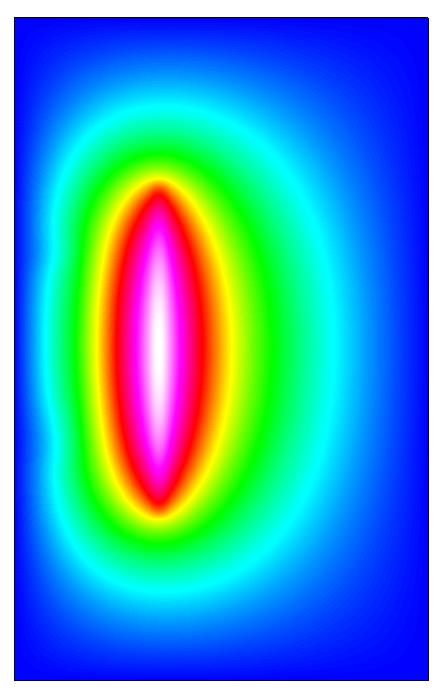
\includegraphics[height=0.4\textwidth]{induct2}
  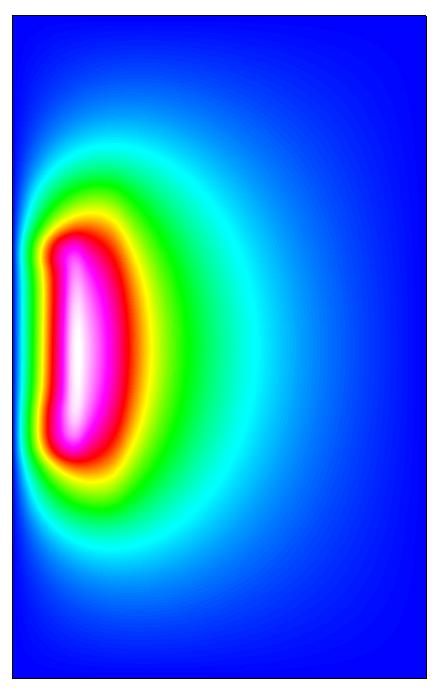
\includegraphics[height=0.4\textwidth]{induct3}
  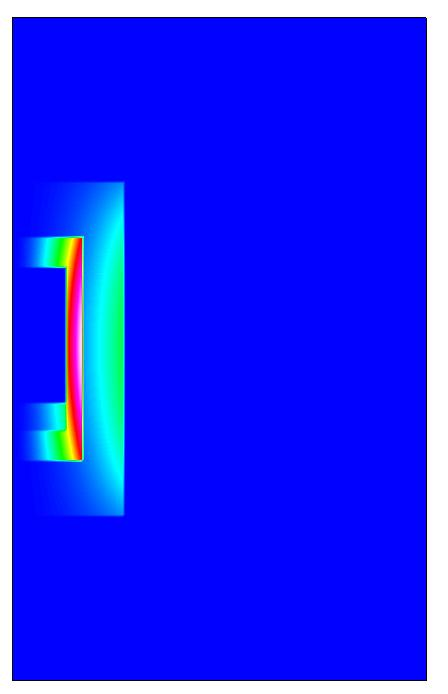
\includegraphics[height=0.4\textwidth]{induct1}
\end{center}
\caption{Induction heating of a simple crucible. 
a) in-phase component of the vector potential
b) out-of-phase component of the vector potential
c) Joule losses in the conductors}
\label{fig:ind_heat1}
\end{figure}



\graphicspath{{./}{FluidStructureBeam/}}
\chapter{Fluid flow around an elastic beam}

\modinfo{Directory}{FluiStructureBeam}
\modinfo{Solvers}{\Idx{ElasticSolve}, \Idx{FlowSolve}, \Idx{MeshSolve}}
\modinfo{Tools}{\Idx{ElmerGrid}, editor, \Idx{Fortran 90 compiler}}
\modinfo{Dimensions}{2D, steady-state}

\subsection*{Case definition}

A homogenous, elastic beam ($\Omega_2$) is in a fluid flow (which takes place
in the region $\Omega_1$), 
see figure~\ref{fg:fsi}. The beam is 5.0~m long and it is rigidly 
supported on the end $\Gamma_6$. At the incoming boundary $\Gamma_1$, the 
fluid velocity in the x-direction is a parabola which reaches its 
maximum value 1~m/s at the point y=5.0~m. At the incoming and outcoming 
boundaries $\Gamma_1$ and $\Gamma_2$ velocities in the y-direction 
are 0~m/s. At the outcoming boundary the pressure is 0~Pa. The velocities 
on boundaries $\Gamma_3$, $\Gamma_4$ and $\Gamma_5$ are 0~m/s. The 
fluid is incompressible and has density 1 kg/m$�$, dynamic 
viscosity 0.5 kg/ms and Poisson ratio 0.3. Material properties 
for the beam are the density 1000~kg/m$�$, Poisson ratio 0.3 and Young's 
modulus 1.0e3~N/m$�$. The problem is to solve the maximum displacement 
of the beam and the pressure change in $\Omega_1$.

\begin{figure}[h]
\centering
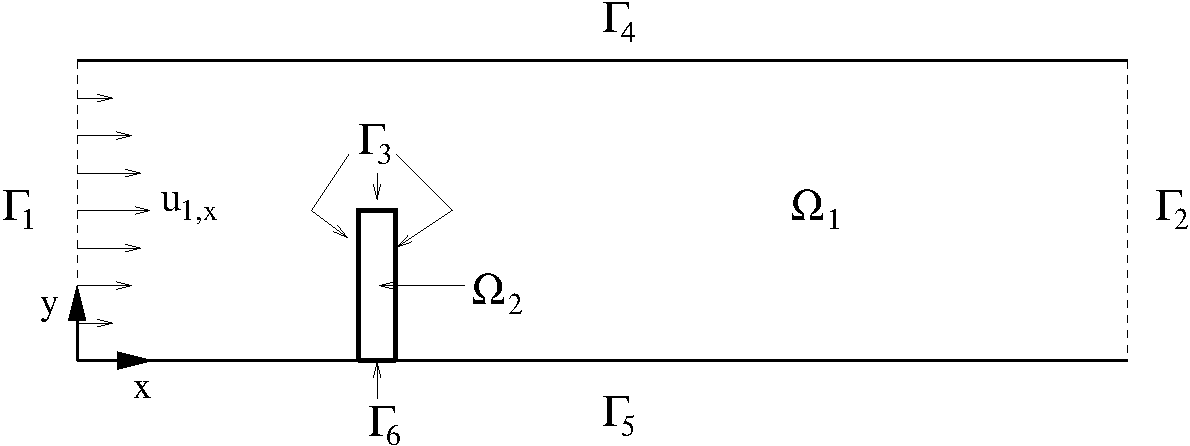
\includegraphics[width=100mm]{fsi}
\caption{Geometry of the problem}\label{fg:fsi}
\end{figure}

The flow generates normal and shear stresses to the beam
boundary $\Gamma_3$. These forces deform the beam and this changes the flow. 
This coupled problem can be modelled using the Navier-Stokes and elasticity 
equations. 

For the incompressible fluid the Navier-Stokes equations can be written as
\begin{equation}
\begin{array}{rcll}
- \nabla \cdot (2 \mu \overline{\overline{\varepsilon}}) + \rho 
\vec{u} \cdot \nabla \vec{u} + \nabla p &=& 0 & \mbox{ in } \Omega_1 \\
\nabla\cdot \vec{u}& = & 0 & \mbox{ in } \Omega_1 \\
\vec{u}_{x} &=& (10y-y^2)/25 & \mbox{ on } \Gamma_1 \\
\vec{u}_{x} &=& 0 & \mbox{ on } \Gamma_i ,\: i=3,4,5 \\
\vec{u}_{y} &=& 0 & \mbox{ on } \Gamma_i ,\: i=1,\ldots,5, 
\end{array}
\end{equation}
where $\mu$ is the dynamic viscosity, $\overline{\overline{\varepsilon}}$ is 
the strain tensor,  $\rho$ is the density, $\vec{u}$ is the velocity vector and
$p$ is the pressure. It is assumed that the density and viscosity are 
constants. 

For the homogeneous, elastic beam the elasticity equations are
\begin{equation}
\begin{array}{rcll}
-div [(I+ \nabla u) \Sigma] &=& 0 & \mbox{ in } \Omega_2 \\
\Sigma &=& \lambda (tr E)I + 2 \mu E & \mbox{ in } \Omega_2 \\
E &=& \frac{1}{2}(\nabla u^{T} + \nabla u + \nabla u^{T} \nabla u) 
& \mbox{ in } \Omega_2 \\
u &=& 0 & \mbox{ on } \Gamma_6 \\
(I+ \nabla u) \Sigma n &=& q & \mbox{ on } \Gamma_3 
\end{array}
\end{equation}
where $u$ is the displacement vector, $\Sigma$ is 
the second Piola-Kirchhoff stress tensor, $\lambda$ and $\mu$ are the Lam\'{e}
constants and $E$ is the Green-St Venant strain tensor, $q$ is the surface 
traction and $n$ is the unit normal to the beam boundary. The edge load $q$ is 
calculated from the stresses obtained using the Navier-Stokes equations.

For updating the fluids mesh a linear elasticity equation is used. In 
mathematical form it can be written as, 
\begin{equation}
\begin{array}{clcr}
-div \{\lambda tr [\varepsilon(v)]I + 2 \mu \varepsilon(v)\} = 0 & 
\mbox{ in } \Omega_1 \\
v = u_{\vert\Gamma_3} & \mbox{ on } \Gamma_3 \\
v = 0 & \mbox{ on } \Gamma_i, i=1,2,4,5 
\end{array}
\end{equation}
where $\lambda$ and $\mu$ are the Lam\'{e} constants, $\varepsilon$ is
linear strain tensor and $v$ is the displacement vector. Here $u$ is the 
solution to the elasticity equations.


\subsection*{Solution procedure}

In this problem geometry and mesh is created by using ElmerGrid by the 
command
\ttbegin
ElmerGrid 1 2 fsi.grd
\ttend

In this problem, external Fortran functions are used to express a
parabolic velocity inflow profile and to define a variable stiffness
for the deforming mesh. The stiffness of the mesh is controlled by the
Youngs modulus. In the case of deforming mesh, the absolute value of
the parameter is not important but its changes over the domain are
influential. The following function defines the mesh to be stiffer
near the corner of the beam where the mesh is deformed most. The idea
is to avoid too irregularly shaped elements in that area.

\ttbegin
FUNCTION Youngs( Model, n, x ) RESULT( s )
  USE Types
  IMPLICIT NONE

  TYPE(Model_t) :: Model
  INTEGER :: n
  REAL(KIND=dp) :: x,s,xx,yy
  
  xx = Model % Nodes % x(n)
  yy = Model % Nodes % y(n)
  
  s =  1.0d0 / SQRT( (xx-11.0)**2 + (yy-4.9)**2 )
  
END FUNCTION Youngs
\ttend

The following function is used to give the inflow boundary condition.

\ttbegin
FUNCTION InFlow( Model, n, x ) RESULT( vin )
  USE Types
  IMPLICIT NONE

  TYPE(Model_t) :: Model
  INTEGER :: n
  REAL(KIND=dp) :: yy,xx,x,vin,v0,vt

  xx = Model % Nodes % x(n)
  yy = Model % Nodes % y(n)
  
  v0 = (-(yy**2)+10*yy)/25
  
  IF(x < 8.0) THEN
    vt = x/8.0
  ELSE
    vt = 1.0
  END IF

  vin = v0*vt

END FUNCTION InFlow
\ttend

In general, the user may supply his/hers own functions for defining
general dependencies of variables or parameters. The function header
should read as follows
\ttbegin
FUNCTION FunctionName( Model, n, x ) RESULT( res )
\ttend
where {\tt Model} is a structure holding various information�of the
problem and {\tt n} is the number of the node being considered. These
are automatically given by the program. The paramter {\tt x} is the
value of the variable, which user defines to be given for the function
as input. The variable is defined in the sif file. Finally, a the
function returns the result {\tt res} for the parameter in
consideration. 

If the Elmer environment is succesfully setup the compilation command 
should look like
\ttbegin
elmerf90 -o FsiStuff FsiStuff.f90
\ttend

The functions may be compiled also locally on a PC either for Linux or
WindowsNT, provided that a Fortran90 compiler and the Elmer software
are installed.

The next step is to edit the solver input file (\texttt{sif} file)
with a text editor, {\em e.g.} Emacs.
\begin{itemize}
\item The Header section, where the mesh is defined. 
%
\ttbegin
Header 
  Mesh DB "." "fsi" 
End
\ttend
%
\item The \texttt{Constants} section need not contain any constant this time.
%
\ttbegin
Constants
End
\ttend
%
\item The \texttt{Simulation} section gives the control data for the case.
%
\ttbegin
Simulation
  Coordinate System = Cartesian 2D
  Simulation Type = Steady State
  Steady State Max Iterations = 50
  Steady State Min Iterations = 2
  Output Intervals = 1
  Output File = "fsi.result"
  Post File = "fsi.ep"
End
\ttend
%
\item The \texttt{Body} section is used to define which equations and
materials are used for the simulation bodies.
($\Omega_2$).
%
\ttbegin
Body 1
  Equation = 1
  Material = 1
End

Body 2 
  Equation = 2 
  Material = 2 
End
\ttend
%
\item The \texttt{Material} section defines the material properties of
each body. Also the procedure \texttt{Youngs} is used. 
%
\ttbegin
Material 1 
  Density = 1.0 
  Viscosity = 0.5 
  Poisson Ratio = 0.3 
  Youngs Modulus = Variable time 
      Real Procedure "FsiStuff" "Youngs" 
End

Material 2
   Density = 1000
   Youngs Modulus = 1.0e3
   Poisson Ratio = 0.3
End
\ttend
%
\item The Solver section defines various control parameters for each 
solver.
%
\ttbegin
Solver 1
  Equation = Navier-Stokes
  Stabilize = True
  Linear System Solver = Iterative
  Linear System Iterative Method = BiCGStab
  Linear System Preconditioning = ILU1
  Linear System Max Iterations = 500
  Linear System Convergence Tolerance = 1.0e-8
  Nonlinear System Max Iterations = 10
  Nonlinear System Convergence Tolerance = 1.0e-5
  Nonlinear System Newton After Tolerance = 1.0e-5
  Nonlinear System Newton After Iterations = 20
  Nonlinear System Relaxation Factor = 1.0
  Steady State Convergence Tolerance = 1.0e-4
End

Solver 2
  Equation = Elasticity Solver
  Variable = Displacement
  Variable DOFs = 2
  Procedure = "ElasticSolve" "ElasticSolver"
  Linear System Solver = Direct
  Linear System Direct Method = Banded
  Nonlinear System Newton After Tolerance = 1.0e-3
  Nonlinear System Newton After Iterations = 20
  Nonlinear System Max Iterations = 100
  Nonlinear System Convergence Tolerance = 1.0e-5
  Nonlinear System Relaxation Factor = 1.0
  Steady State Convergence Tolerance = 1.0e-4
End

Solver 3 
  Equation = Mesh Update
  Linear System Solver = Iterative
  Linear System Iterative Method = BiCGStab
  Linear System Preconditioning = ILU1
  Linear System Max Iterations = 500
  Linear System Convergence Tolerance = 1.0e-8
  Steady State Convergence Tolerance = 1.0e-4
End
\ttend
%
\item The \texttt{Equation} section. This section defines the
equations for a body. Plane stress model for the elastic beam is 
applied. Setting this keyword to {\tt False} enables the plane 
strain assumption.
%
\ttbegin
Equation 1
  Active Solvers(2) = 1 3
End

Equation 2
  Active Solvers = 2
  Plane Stress = True
End
\ttend
%
\item In the \texttt{Boundary Condition} section different boundary
conditions are defined.  In Boundary Condition~1 the shape of inflow
is defined with the Fortran procedure \texttt{InFlow}. Note also the
bc 3, where keyword {\tt FSI BC} is supplied to define the boundary on
which the fluid affects a force on the elastic beam. Also, on the same
boundary, the mesh is constraint to follow the deformation of the beam
by the two Equals lines.
%
\ttbegin
Boundary Condition 1 
  Target Boundaries = 1
  Velocity 1 = Variable Time
      Real Procedure "FsiStuff" "InFlow"

  Velocity 2 = 0.0
  Mesh Update 1 = 0.0
End 

Boundary Condition 2
  Target Boundaries = 2
  Velocity 2 = 0.0
  Pressure = 0.0
  Mesh Update 1 = 0.0
End

Boundary Condition 3 
  Target Boundaries = 3
  Velocity 1 = 0.0
  Velocity 2 = 0.0
  FSI BC = True
  Mesh Update 1 = Equals Displacement 1
  Mesh Update 2 = Equals Displacement 2
End

Boundary Condition 4
  Target Boundaries(2) = 4 5
  Velocity 1 = 0.0
  Velocity 2 = 0.0
  Mesh Update 2 = 0.0
End

Boundary Condition 5
  Target Boundaries = 6 
  Displacement 1 = 0.0
  Displacement 2 = 0.0
End
\ttend
%
\end{itemize}

\subsection*{Results}

After the solution is done, view the results with ElmerPost. 
Read the result file fsi.ep in ElmerPost by choosing Read Model File. The 
fsi.ep file is located in the same directory as the mesh files. 

\begin{table}[tbhp]
\caption{Max. displacement and pressure difference}
\label{tb:struct5}
\begin{center}
\begin{tabular}{lll} \hline
Elements & $\max |u|$ [m] & $\max \Delta p$ [Pa] \\  \hline 
540  &  1.34  &  6.36  \\ \hline 
\end{tabular}
\end{center}
\end{table}

As a result the maximum absolute value of displacement and the 
pressure difference is given (see table~\ref{tb:struct5}).


\graphicspath{{./}{ThermalActuator/}}
\chapter{Thermal actuator driven with electrostatic currents}

\modinfo{Solvers}{\Idx{StatCurrentSolve}, \Idx{HeatSolve}, 
	\Idx{StressSolve}}
\modinfo{Tools}{\Idx{ElmerGrid}, editor}
\modinfo{Dimensions}{3D, Steady-state}

\subsection*{Case definition}

The tutorial introduces a micro mechanical thermal actuator as shown
in Fig.~\ref{geom_thermal}. A static electric current is driven
through the actuator. The power loss due to the resistance of the
actuator is transformed into heat which in turn causes thermal
stresses into the structure. The electric current thus results in
deformation of the actuator. In industry, such an actuator might be
used to control the position of a micromechanical component.

\begin{figure}[h]
  \centerline{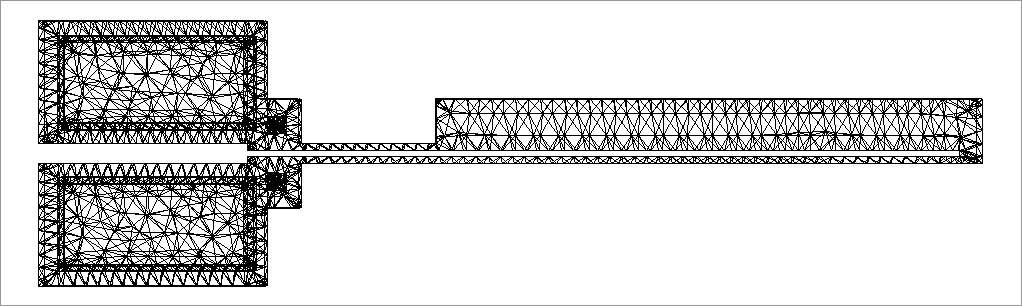
\includegraphics[width=0.8\textwidth]{geometry_wh}}
  \caption{The geometry of the actuator.} 
  \label{geom_thermal}
\end{figure}


\subsection*{Solution procedure}

The problem is solved by first iterating the electrostatic current
solver and heat equation until both are converged. The temperature
distribution is then used as a load for stress analysis solver which
calculates the actual deformation of the structure. The electric
conductivity of the actuator depends on the temperature and thus the
electrostatic - thermal problem is coupled in both directions.

The computational mesh for this particular tutorial is created by
using \Idx{Ansys} software. The details of the mesh are written into
files called \texttt{ExportMesh} by a certain Ansys macro and
converted to Elmer format by the ElmerGrid program. The command to use
is
\ttbegin
ElmerGrid 4 2 ExportMesh -order 1.0 0.1 0.001 -o thermal
\ttend 
The above command reads in the Ansys mesh files, arranges the mesh 
nodes in a reasonable way and saves the mesh in Elmer format in a
directory called \texttt{thermal}.

The geometry of the problem includes only one body and
material. Boundary conditions are defined on the actuator legs, which
are kept at constant electric potential, temperature and
position. Thus, only Dirichlet boundary conditions are used.

The header and simulation blocks of the solver input file are

\ttbegin
Header
  Mesh DB "." "thermal"
End

Simulation
  Coordinate System = Cartesian 3D
  Simulation Type = Steady State
  Steady State Max Iterations = 30
  Output Intervals = 1
  Output File = "actuator.result"
  Post File = "actuator.ep"
End
\ttend

An initial condition for temperature is defined in order to ease the
convergence of the iterative solvers. Also, a body force for the
heat equation solver defining the Joule heating is needed. These
both have to be declared in the body section as follows:

\ttbegin
Body 1
  Equation = 1
  Material = 1
  Initial Condition = 1
  Body Force = 1
End
\ttend

The solution procedure requires the use of three solvers: Static
current solver, heat equation solver and the stress analysis
solver. The equation block below defines that these solvers are
used. 

\ttbegin
Equation 1
  Active Solvers(3) = Integer 1 2 3
  Calculate Joule Heating = True
End
\ttend

The solver blocks define the parameters of the respecting solvers. The
static current conduction problem is tackled by an iterative conjugate
gradient method (CG). For heat equation, a stabilized biconjugate
gradient method is used. The coupled problem of these two solvers is
difficult since the static current calculated heats the structure on
each step, and the rise of temperature makes the current conduction
more and more difficult. To overcome this problem, a relaxation factor
of 0.5 is defined for the heat equation solver.

\ttbegin
Solver 1
  Equation = Stat Current Solver
  Procedure = "StatCurrentSolve" "StatCurrentSolver"
  Variable = Potential
  Variable DOFs = 1
  Calculate Volume Current = True
  Calculate Electric Conductivity = True
  Linear System Solver = Iterative
  Linear System Iterative Method = CG
  Linear System Preconditioning = ILU3
  Linear System Max Iterations = 300
  Linear System Convergence Tolerance = 1.0e-8
  Nonlinear System Max Iterations = 1
  Nonlinear System Convergence Tolerance = 1.0-6
  Nonlinear System Newton After Iterations = 3
  Nonlinear System Newton After Tolerance = 1.0e-12
  Nonlinear System Relaxation Factor = 1.0
  Steady State Convergence Tolerance = 1.0e-6
End

Solver 2
   Equation = Heat Equation
   Variable = Temperature
   Variable DOFs = 1
   Linear System Solver = Iterative
   Linear System Iterative Method = BiCGStab
   Linear System Preconditioning = ILU1
   Linear System Max Iterations = 350
   Linear System Convergence Tolerance = 1.0e-9
   Nonlinear System Max Iterations = 1
   Nonlinear System Convergence Tolerance = 1.0e-07
   Nonlinear System Newton After Iterations = 3
   Nonlinear System Newton After Tolerance = 1.0e-12
   Nonlinear System Relaxation Factor = 0.5
   Steady State Convergence Tolerance = 1.0e-07
End
\ttend

For stress analysis, a direct solver is used instead of an iterative
solver. It is often difficult for the iterative solver to find a
solution for a structure that contains parts with varying stiffness
properties, which is obviously the case here (try the iterative solver
and see!). The stress analysis solver is called first only after the
coupled iteration of two previous solvers is complete. This is
possible since the deformation of the structure is so small that it
does not change the current density distribution. Defining stress
analysis this way saves computational time. It is possible to
iterate all the three solvers until convergence by commenting the
\texttt{Exec Solver} line.

\ttbegin
Solver 3
  Exec Solver = After All
  Equation = Stress Analysis
  Variable = Displacement
  Variable DOFs = 3
  Linear System Solver = Direct
  Linear System Direct Method = Banded
  Nonlinear System Max Iterations = 1
  Nonlinear System Convergence Tolerance = 1.0e-6
  Nonlinear System Newton After Iterations = 3
  Nonlinear System Newton After Tolerance = 1.0e-12
  Nonlinear System Relaxation Factor = 1.0
  Steady State Convergence Tolerance = 1.0e-6
End
\ttend

The material of the structure has a temperature dependent electric
conductivity. This, as well as other material parameters, is defined
in the material block. Note that a MEMS unit system is used.

\ttbegin
Material 1
  Electric Conductivity = Variable Temperature
      Real
        298.0   4.3478e10
        498.0   1.2043e10
        698.0   5.1781e9
        898.0   2.7582e9
        1098.0  1.6684e9
        1298.0  1.0981e9
        1683.0  1.0
        2000.0  1.0
      End

  Density = 2.3e-15
  Heat Conductivity = 32.0e6
  Youngs Modulus = 169.0e3
  Poisson Ratio = 0.22
  Heat Expansion Coefficient = 2.9e-6
  Reference Temperature = 298.0
End
\ttend

Finally, the initial condition, thermal heat load for stress analysis,
and the boundary conditions are defined.

\ttbegin
Initial Condition 1
   Temperature = 298.0
End

Body Force 1
  Heat Source = Equals Joule Heating
End

Boundary Condition 1
  Target Boundaries = 1
  Potential = 0
  Temperature = 298
  Displacement 1 = 0.0
  Displacement 2 = 0.0
  Displacement 3 = 0.0
End

Boundary Condition 2
  Target Boundaries = 2
  Potential = 7
  Temperature = 298
  Displacement 1 = 0.0
  Displacement 2 = 0.0
  Displacement 3 = 0.0
End
\ttend

\subsection*{Results}

The problem converges after 27 steady state iterations on the
tolerance limits defined above. The calculation takes about 180 cpu
seconds of which 40 cpus is spent in solving the stress analysis
equation. The calculations were performed on a Compaq Alpha Server
with a 1 GHz central processor.

\begin{figure}[tbhp]
  \centerline{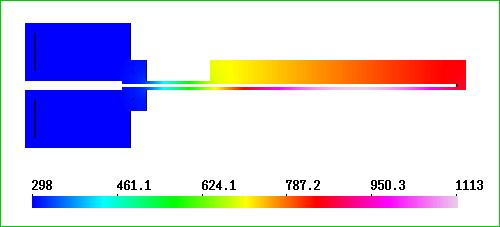
\includegraphics[width=0.8\textwidth]{temp_wh}}
  \caption{Temperature distribution.} 
  \label{temp_thermal}
\end{figure}
\begin{figure}[h]
  \centerline{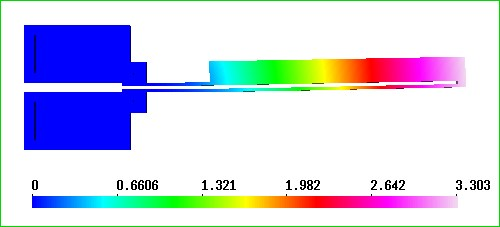
\includegraphics[width=0.8\textwidth]{displ_wh}}
  \caption{The displacement of the actuator.} 
  \label{displ_thermal}
\end{figure}

Result for temperature distribution and the displacement are shown in
Figs~\ref{temp_thermal} and~\ref{displ_thermal}. The temperature rises
unrealistically high in this example because all heat transfer
mechanisms out of the structure are neglected. Presumambly at least
the heat radiation is of major importance in this case. For
displacement, the results show a movement of about 3.3 micrometers for
the actuator tip.

\vfill
\mbox{}


\graphicspath{{./}{CoatingProcess/}}
\chapter{Axisymmetric coating process}

\modinfo{Solvers}{\Idx{FlowSolve}, \Idx{FreeSurfaceReduced}}
\modinfo{Tools}{\Idx{ElmerGrid}, editor}
\modinfo{Dimensions}{2D, Steady-state}

\subsection*{Case definition}

The optical fibers are quite fragile and must therefore be coated with
a layer of polymer before they are stored.  This means that the
coating process must be done with the same speed as the drawing of
optical fibers.  When the diameter of the fiber is only 125 $\mu$m
this sets high demands for the coating geometry since it must provide
even coating at high draw speeds. In Elmer a tailored free surface
boundary condition allows an efficient solution of this particular
problem.


\subsection*{Solution procedure}

The mesh is done with ElmerGrid in the directory coat by the command
%
\ttbegin
ElmerGrid 1 2 coat.grd
\ttend

Therefore the header reads 
\ttbegin
Header
  Mesh DB "." "coat"
End
\ttend
%
The geometry is axisymmetric and the problem is solved in steady state. Typically around 10
iterations is needed to solve the problem but to be on the safe side 30 is set as the maximum.
\ttbegin
Simulation
  Coordinate System = Axi Symmetric
  Simulation Type = Steady State
  Steady State Max Iterations = 30
  Output Intervals = 1
  Output File = "coat.result"
  Post File = "coat.ep"
End
\ttend
%
In this case there is only one body which comprises of the polymer 
floating between the coating cup and the optical fiber.
\ttbegin
Body 1
  Equation = 1
  Material = 1
End
\ttend

The presented solution used four different solvers. 
The Navier-Stokes solver is required to solve the flow field
for the polymer.
\ttbegin
Solver 1
  Equation = Navier-Stokes
  Stabilize = True
  Internal Move Boundary = Logical False
  Nonlinear System Max Iterations = 5
  Nonlinear System Convergence Tolerance = 1.0e-7
  Nonlinear System Newton After Iterations = 2
  Nonlinear System Newton After Tolerance = 1.0e-2
  Nonlinear System Relaxation Factor = 0.7
  Linear System Solver = Iterative
  Linear System Iterative Method = BiCGStab 
  Linear System Preconditioning = ILU1
  Linear System Max Iterations = 100
  Linear System Convergence Tolerance = 1.0e-10
  Steady State Convergence Tolerance = 1.0e-7
End
\ttend
%
A tailored free surface solver is used to find the 
position of the free surface with a given flow field.
The variable being solved is the displacement of the free surface.
Relaxation is used to avoid over-shooting during the itaration.
This solver does not solve any matrix equations. Instead it solves
the radius from the mass conservation constraint for each node on the
free surface separately. There is a possibility to do the mapping also 
within the solver using a 1D scheme but this is disabled by setting
the \texttt{Perform Mapping} to be \texttt{False}.
\ttbegin
Solver 2
  Equation = "Free Surface Reduced"
  Procedure = "FreeSurfaceReduced" "FreeSurfaceReduced"
  Variable = Dx
  Variable DOFs = 1
  Nonlinear System Relaxation Factor = 0.7
  Nonlinear System Convergence Tolerance = 1.0e-3
  Steady State Convergence Tolerance = 1.0e-3
  Perform Mapping = Logical False
End
\ttend
%
The mesh update solver is required to map the computational mesh
so that it corresponds to the altered geometry.
Here the displacements of the free surface have already been computed
and this solver solves the displacements inside the domain.
Note that solvers 1, 2 and 3 are coupled and therefore the system must be solved iteratively
\ttbegin
Solver 3
  Equation = Mesh Update
  Linear System Solver = Iterative 
  Linear System Iterative Method = BiCGSTAB
  Linear System Preconditioning = ILU
  Linear System Convergence Tolerance = 1.0e-12
  Linear System Max Iterations = 200
  Linear System Symmetric = True
  Steady State Convergence Tolerance = 1.0e-4
End
\ttend
%
In the end, an additional solver is used to compute the forces
acting on the fiber. This does not affect the results.
\ttbegin
Solver 4 
  Equation = Fluidic Force
  Procedure = "FluidicForce" "ForceCompute"
  Calculate Viscous Force = Logical True
End
\ttend
%
Addiationally there are two solvers for saving the results in a form
that is more useful than plain pictures. The \texttt{SaveScalars} saves
the scalar values, such as the diameter and force values,
and the \texttt{SaveLine} saves the free surface.
\ttbegin
Solver 5
  Equation = SaveScalars
  Procedure = "SaveData" "SaveScalars"
  Filename = "scalars.dat"
End 

Solver 6
  Equation = SaveLine
  Procedure = "SaveData" "SaveLine"
  Filename = "kurvi.dat"
End
\ttend
%
The equation includes only the solvers that need a permutation vector 
pointing out the active nodes. Therefore the save utilities do not need to belong
to the set of active solvers.
\ttbegin
Equation 1
  Active Solvers(4) = 1 2 3 4
End
\ttend
%
The material parameters are those of the polymer. Additionally elasticity 
parameters are needed because the solver that updates the mesh is actually
a linear elasticity solver.
\ttbegin
Material 1
  Density = 1.0
  Viscosity = 1.0
  Poisson Ratio = 0.3
  Youngs Modulus = 1.0
End
\ttend

Five different boundary conditions are needed.
The origin is a symmetry axis and thefore the radial velocity is 
set to zero. The axial velovity is the draw velocity.
\ttbegin
Boundary Condition 1
  Name = "Symmetry"
  Target Boundaries = 1
  Velocity 2 = -10.0     ! The draw velocity
  Velocity 1 = 0.0
  Compute Fluidic Force = Logical True
  Mesh Update 1 = 0.0
End
\ttend
%
The free surface has a condition stating that the reduced order free 
surface solver should be solved for that. Additionally the 
free surface is a boundary condition for the mesh update,
and a line to be saved.
\ttbegin
Boundary Condition 2
  Name = "Free"
  Target Boundaries = 2
  Mesh Update 1 = Equals Dx
  Mesh Update 2 = 0.0
  Free Surface Reduced = Logical True
  Save Line = Logical True
End
\ttend
%
At the outlet the radial velocity should vanish and the axial coordinate should
be fixed.
\ttbegin
Boundary Condition 3
  Name = "Outlet"
  Target Boundaries = 3
  Velocity 1 = 0.0
  Mesh Update 2 = 0.0
End
\ttend
%
At the inlet it is assumed that there is no radial velocity and that 
the pressure acting on the surface is zero.
\ttbegin
Boundary Condition 4
  Name = "Inlet"
  Target Boundaries = 4
  Velocity 1 = 0.0
  Pressure = 0.0
  Mesh Update 2 = 0.0
End
\ttend
%
Finally, no-slip conditions are set for the boundaries with the walls of the
coater.
\ttbegin
Boundary Condition 5
  Name = "No-slip"
  Target Boundaries = 5
  Velocity 1 = 0.0
  Velocity 2 = 0.0
  Mesh Update 1 = 0.0
  Mesh Update 2 = 0.0
End
\ttend


\subsection*{Results}

\begin{figure}[tbhp]
\begin{center}
  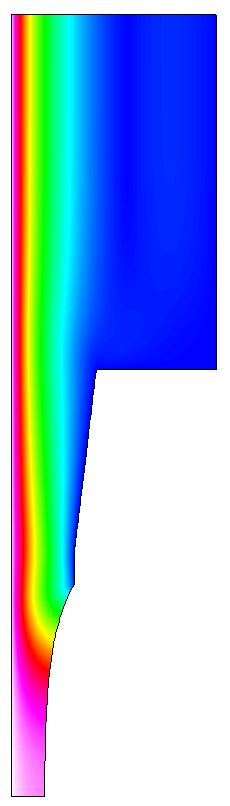
\includegraphics[height=0.6\textwidth,angle=0]{coat_vel}
  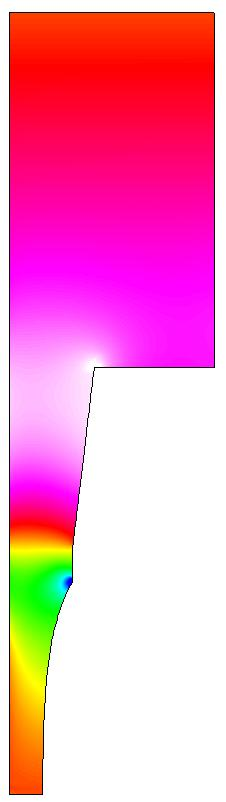
\includegraphics[height=0.6\textwidth,angle=0]{coat_pres}
  \caption{The velocity and pressure fields in a simple coating geometry.
	The solution utilizes the reduced dimensional free surface solver.}
\end{center}
\end{figure}

In the given case solution is obtained after 13 iterations.
The solution gives the final radius, the forces, and the profile of the 
free surface. To visualize the true free surface you may do the following.
Read in the only the last timestep and in \texttt{ElmerPost} give the following
commands:
\ttbegin
math nodes0 = nodes
math nodes = nodes0 + Mesh.Update
\ttend
Note that this does not work if there is more than one set of variable values.


\vfill
\mbox{}


\graphicspath{{./}{FlowResistance/}}
\chapter{Flow through a hole -- determining the acoustic impedance} 

\modinfo{Directory}{FlowResistance}
\modinfo{Solvers}{\Idx{FlowSolve}}
\modinfo{Tools}{\Idx{ElmerGrid}, editor}
\modinfo{Dimensions}{3D, Steady-state}

\subsection*{Case definition}

The problem at hand consists of finding the resistance that a fluid
faces as it is forced to flow through a hole. The flow resistance is
stated by the ratio of pressure drop over the hole and the input
velocity. In microsystem modeling, the hole resistance is often needed
to analyse the gas damping effect in perforated structures. Here, the
contribution of the holes is homogenised over the perforated structure
based on a single hole resistance. For homogenisation in Elmer, the
specific \Idx{acoustic impedance} is used to represent the flow
resistance. Specific acoustic impedance $z_h$ is defined as
\begin{equation}
z_h = \frac{p}{v} = \frac{F}{vA_h},
\end{equation}
where $F$ is the net force due to gas on the moving surface, $v$ is
the velocity of the gas on the same surface, and $A_h$ is the area of
the moving surface. The calculation is best performed in a unit cell
of the geometry.

In order to the homogenisation to be possible, the dependence of input
velocity and the net force should be linear. Further, there should not
be a phase change between these two quantities. These conditions are
satisfied when the flow is incompressible.  In a linear case, the
fluid flow can be treated with the linear form of Navier-Stokes
equations called the \Idx{Stokes equation}
\begin{equation}
\rho\frac{\partial \vec{u}}{\partial t}
-\nabla\cdot(2\eta\overline{\overline{\varepsilon}}) +\nabla p =
\rho \vec{f},
\end{equation}
where $\vec{u}$ is the unknown velocity field, $p$ is the pressure,
$\eta$ is the viscosity of the fluid, $\rho\vec{f}$ is a body force
and $\overline{\overline{\varepsilon}}$ is the linearised strain
tensor. Note, that the stationary version of the above equation can be
used in homogenisation calculations.

The condition for Stokes equation to apply is that the Reynolds number
$Re$ of the problem should be small
\begin{equation}
Re = \frac{\rho UL}{\eta},
\end{equation}
where $\rho$ is density of the fluid and $U$ and $L$ are,
respectively, the velocity and length scales of the problem.

The issue of compressibility is more difficult to answer. A classical
condition for the compressibility is that the Mach number $Ma$ of the
problem should be small
\begin{equation}
Ma = \frac{U}{a} < 0.3,
\end{equation}
where $a$ is the speed of sound in the gas in operating conditions and
the value~0.3 is often stated limit for a small Mach number (actually,
the condition is that $Ma^2$ has to be small).  Also the frequency and
amplitude of the oscillations of the system have an effect on the
validity of the linearity and incompressibility assumptions, since
they affect the velocity scale of the problem.

However, also other factors have an effect on the compressibility of
the gas. In microsystems, the viscous effects on pressure, or even
temperature changes, can affect the density of the gas. A
condition for viscous pressure changes is that $Ma^2/Re$ has to be
small, and for temperature, in addition, that the Prandtl number $Pr$
may not be too large
\begin{equation}
Pr = \frac{\eta c_p}{k},
\end{equation}
where $c_p$ is the heat capacity ({\em ie.} specific heat) in constant
pressure and $k$ is the thermal conductivity.

The conditions listed here for the flow to be approximately
incompressible are only an overview and the validity of
incompressibility assumption should be considered in each case
separately. In microsystems, refer for example to the article
M.~Gad-el-Hak, J.~Fluids Eng., 121, 5--33, 1999. Additionally, it is
advisable to perform numerical checks on the issue.

One final point on the applicability of the Stokes (or Navier-Stokes)
equations is the effect of gas rarefication. If the dimensions of the
problem are very small the continuity assumption may not be valid
anymore. The importance of the gas rarefication effects are given by
the Knudsen number $Kn$
\begin{equation}
Kn = \frac{{\cal L}}{L},
\end{equation}
where ${\cal L}$ is the mean free path of the gas molecules. The mean
free path depends inversely on ambient pressure, which has to take
into account in stating the Knudsen number. For Knudsen numbers close
to and less than~1, slip boundary conditions should be used.

To summarise, the motivation of this tutorial is to perform a linear
incompressible simulation of fluid flowing through a hole. The wake
for the flow is a constant velocity boundary condition for a boundary
before the hole. On the same boundary, the force caused by the fluid
is recorded. These two quantities can then be used to determine the
specific acoustic impedance of a single hole. The constant velocity
boundary condition may be interpreted as describing a moving wall with
small displacement. In this particular tutorial, a symmetrical
quadrant of a square-shaped hole is used.



\subsection*{Solution procedure}

The solution for the problem is found by solving iteratively the
Stokes equation. Nonlinear iterations are not needed, since the
problem is linear.

The computational mesh should include enough free space after the hole
so that any artificial effects due to the boundaries of the mesh are
avoided. In this tutorial, the geometry is created and meshed using
the ElmerGrid program by the command
{\tt
elmergrid 1 2 hole.grd}. 
The default mesh consists of about 12000 nodes and 10500 eight-noded
hexahedrons.

The header section of solver input file includes only the location of
the mesh files.
\ttbegin
Header
  Mesh DB "." "hole"
End
\ttend

In the simulation section, a steady-state three-dimensional analysis
is defined.
\ttbegin
Simulation
  Coordinate System = Cartesian 3D
  Simulation Type = Steady State
  Steady State Max Iterations = 1
  Output File = "flow.result"
  Post File = "flow.ep"
End
\ttend

The geometry contains only one body and no body forces or initial
conditions are present. The body section reads thus as follows.
\ttbegin
Body 1
  Equation = 1
  Material = 1
End
\ttend

For solving the flow patterns the Navier-Stokes solver is used but the
nonlinearity through convection is switched off in the equation block.
Also, solvers for the fluidic force and saving data are enabled.
\ttbegin
Equation 1
  Active Solvers(3) = Integer 1 2 3
  NS Convect = False
End
\ttend

Just a single iteration of the Navier-Stokes solver is needed, since
the equation is linear. This can be verified by switching the number
of nonlinear iterations to a value more than one, and observing the
change in solution between iteration steps.
\ttbegin
Solver 1
   Equation = Navier-Stokes
   Variable = Flow Solution
   Variable DOFs = 3
   Linear System Solver = Iterative
   Linear System Iterative Method = BiCGStab
   Linear System Preconditioning = ILU0
   Linear System Max Iterations = 200
   Linear System Convergence Tolerance = 1.0e-08
   Stabilize = True
   Nonlinear System Convergence Tolerance = 1.0e-05
   Nonlinear System Max Iterations = 1
   Nonlinear System Newton After Iterations = 3
   Nonlinear System Newton After Tolerance = 1.0e-08
   Nonlinear System Relaxation Factor = 1.0
   Steady State Convergence Tolerance = 1.0e-05
End
\ttend

The fluidic force solver needs to be run only once, after the flow
solution is finished. With the keyword {\tt Calculate Viscous Force} it
is possible to define whether the viscous forces of the fluid are
included in the force or not. If this is set to false, only the
pressure integral is calculated.
\ttbegin
Solver 2
  Exec Solver = After All
  Equation = Fluidic Force
  Procedure  ="FluidicForce" "ForceCompute"
  Calculate Viscous Force = True
End
\ttend

The final solver is used to save data from the analysis. With the
following definitions, the input velocity and the net force on the
input boundary as well as the area of the boundary are written into a
file called {\tt flowdata.dat}.
\ttbegin
Solver 3
  Exec Solver = After All
  Equation = SaveScalars
  Procedure = "\Idx{SaveData}" "SaveScalars"
  Filename = "flowdata.dat"
  Save Variable 1 = Velocity 3
  Save Coordinates(1,2) = 0.0 0.0
End
\ttend

The fluid is defined to be air. Note the Elmer \Idx{MEMS} units used.
\ttbegin
Material 1
  Name = Air
  Density = 1.293e-12
  Viscosity = 1.67e-5
End
\ttend

Finally, the boundary conditions. BC~1 defines the input boundary,
where also the fluidic force is calculated. BCs~2 and~4 are define the
symmetry boundaries, BC~3 defines the no-slip conditions for the
walls, and BC~5 defines an open boundary.
\ttbegin
Boundary Condition 1
  Target Boundaries = 4
   Velocity 1 = 0.0
   Velocity 2 = 0.0
   Velocity 3 = 1.0e3
   Calculate Fluidic Force = True
End

Boundary Condition 2
  Target Boundaries(2) = 8 10
   Velocity 2 = 0.0
End

Boundary Condition 3
  Target Boundaries(4) = 1 2 3 7
   Velocity 1 = 0.0
   Velocity 2 = 0.0
   Velocity 3 = 0.0
End

Boundary Condition 4
  Target Boundaries(2) = 6 9
   Velocity 1 = 0.0
End

Boundary Condition 5
  Target Boundaries = 5
  Pressure = 0.0
End
\ttend

\subsection*{Slip boundary conditions}

The same simulation can also be performed using slip boundary
conditions. These are appropriate, as stated in introduction, when the
Knudsen number is between $10^{-3}$ and 1. The slip boundary condition
implemented in Elmer is of first order 
\begin{equation}
S\cdot \vec{u} = \overline{\overline{\sigma}}\cdot\vec{n},
\end{equation}
where $S$ is a vector containing the slip coefficients $s_i$ for each
velocity component, $\mu$ is the viscosity, and
$\overline{\overline{\sigma}}$ is the stress tensor. For Newtonian
fluids and for tangential directions of the boundary this gives
\begin{equation}
s_i u_i = \mu\frac{\partial u_i}{\partial n},
\end{equation}
where $s_i$ and $u_i$ refer to the same tangential component of the
slip coefficient and the flow velocity.

The value of the slip coefficient is related to the mean free path of
the gas molecules $\lambda$. For example, Maxwell's first order slip
boundary condition may be used (as in {\em e.g.} A.~Beskok, {\em
Num. Heat Transfer,} B, 40, 451--471, 2001):
\begin{equation}
u_i = \frac{2-\sigma_v}{\sigma_v}\lambda 
\frac{\partial u_i}{\partial n},
\end{equation}
where $\sigma_v$ is the tangential momentum accommodation coefficient,
which models the momentum exchange of gas molecules and the
surface. The accommodation coefficient is dependent on the gas and on
the surface, and recent measurements give a result of $\sigma_v\simeq
0.80$ for various monoatomic gases such as Argon in contact with
prime Silicon crystal. 

The slip coefficient of Elmer can finally be written as
\begin{equation}
s_i = \frac{\mu}{\lambda}\frac{\sigma_v}{2-\sigma_v}.
\end{equation}
The mean free path is defined as
\begin{equation}
\lambda = \frac{\mu}{\rho}\sqrt{\frac{\pi M}{2RT}}_,
\end{equation}
where $\rho$ is density, $M$ is the molar mass, $T$ is the
temperature, and $R=8.3145$~J/mol~K is the molar gas constant.

In the Elmer analysis, only a few changes in the sif-file are needed
to make the slip conditions active. The flow force boundary conditions
have to be turned on and the numerical value of the slip coefficient
has to be defined on each boundary (here $s=$2e-4 is used for
air). Further below is a list of the Boundary Condition blocks. Note
that there are more BCs than in the no-slip simulation, since a
separate condition is needed for surfaces oriented differently in
space.

Generally, a normal-tangential orientation scheme for the boundary
conditions are needed, since the surfaces are not necessarily having a
normal vector pointing in one of the coordinate directions. This would
be done for each such boundary by the line
\ttbegin
  Normal-Tangential Velocity = True
\ttend
after which the Velocity component~1 points to the normal direction
and the other components to the tangential directions.

\ttbegin
! Definitions for slip boundary conditions:
Boundary Condition 1
  Target Boundaries = 4
   Flow Force BC = True
   Slip Coefficient 1 = 2e-4
   Slip Coefficient 2 = 2e-4
   Velocity 3 = 2.0e3
   Calculate Fluidic Force = True
End

Boundary Condition 2
  Target Boundaries(2) = 8 10
   Velocity 2 = 0.0
End

Boundary Condition 3
  Target Boundaries(2) = 2 3
   Flow Force BC = True
   Velocity 3 = 0.0
   Slip Coefficient 1 = 2e-4
   Slip Coefficient 2 = 2e-4
End

Boundary Condition 4
  Target Boundaries(2) = 6 9
   Velocity 1 = 0.0
End

Boundary Condition 5
  Target Boundaries = 5
  Pressure = 0.0
End

Boundary Condition 6
  Target Boundaries = 1
   Flow Force BC = True
   Velocity 1 = 0.0
   Slip Coefficient 2 = 2e-4
   Slip Coefficient 3 = 2e-4
End

Boundary Condition 7
  Target Boundaries = 7
   Flow Force BC = True
   Velocity 2 = 0.0
   Slip Coefficient 1 = 2e-4
   Slip Coefficient 3 = 2e-4
End
\ttend

\subsection*{Results}

The computation takes about 200~cpu seconds on an AlphaServer with
1~GHz central processor when trilinear elements are used. The results
for two different input velocities taken from the file {\mbox{\tt
flowdata.dat}} are summarised in Table~\ref{tab:imped_res}. Also the
specific acoustic impedance $z_h$ is calculated in the table. The
results of slip and no-slip simulations are also compared.  Note that
for the force, only the component perpendicular to the surface should
be used since the other components cancel out due to symmetry. The
values in the table are again given in Elmer MEMS units.
\begin{table}[htb]
\caption{Results of flow simulations for two input velocities}
\label{tab:imped_res}
\begin{center}
\begin{tabular}{cccc} \hline
$v$ & \ \ slip model\ \  & $F_z$ & $z_h$ \\ \hline 
$1.0\cdot 10^3$   & no-slip  & 36.13  &  $1.45\cdot10^{-3}$ \\
$2.0\cdot 10^3$   & no-slip  & 72.25  &  $1.45\cdot10^{-3}$ \\ \hline
$1.0\cdot 10^3$   & slip     & 29.30  &  $1.17\cdot10^{-3}$ \\
$2.0\cdot 10^3$   & slip     & 58.60  &  $1.17\cdot10^{-3}$ \\ \hline
\end{tabular}
\end{center}
\end{table}

The identical values obtained for the spesific acoustic impedance in
Table~\ref{tab:imped_res} prove by no means that the flow in reality
is linear, since this was the assumption and the simulation performed
can and should not reveal any nonlinear behavior. The results
indicate, though, that allowing slip on the boundaries reduces the
resistance that the fluid faces. This example shows that in
microsystems, as the dimension of the smallest flow channel is in the
range of a micrometer, it is reasonable to use slip boundary
conditions for the velocity.

\begin{figure}[htb]
  \centerline{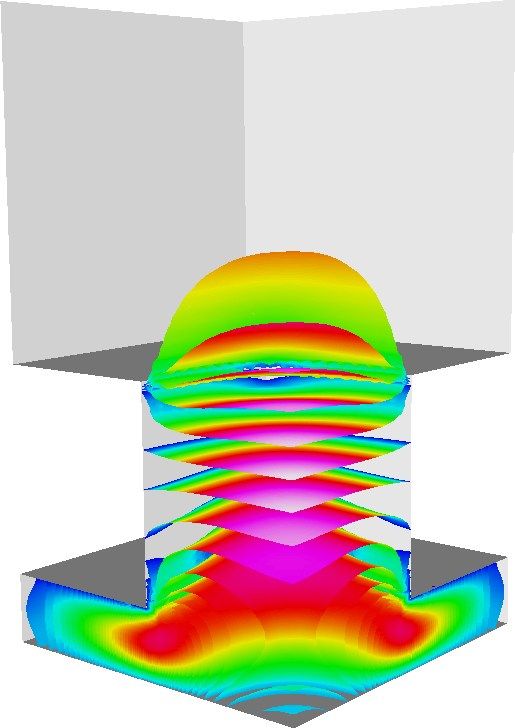
\includegraphics[width=0.40\textwidth]{flow_res}}
  \caption{The linear flow results.} 
  \label{fig:flow_res}
\end{figure}
Finally, a picture of the results obtained with no-slip conditions is
presented. The Fig.~\ref{fig:flow_res} shows a lot of pressure
isosurfaces which are coloured using the absolute value of the
velocity.


\vfill
\mbox{}


\graphicspath{{./}{ArteryFlow/}}
\chapter{Blood ejection from a ventricle into aorta}

\modinfo{Directory}{ArteryFlow}
\modinfo{Solvers}{\Idx{FlowSolve},\Idx{ElasticSolve}, \Idx{OutletCompute}} 
\modinfo{Tools}{Editor, \Idx{Fortran 90 compiler}, \Idx{ElmerGrid}}
\modinfo{Dimensions}{2D, Transient}

\subsection*{Case description}

This tutorial is about simulating blood ejection in to the elastic human aorta.
The idea is to mimic left ventricle contration and resulting pulse propagation 
in an elastic conduit. In the simulation about 0.8 
desiliters of blood is ejected to a 50 cm long elastic aorta during a time 
period of 400 ms.  In order to get the outlet of the model behave 
physiologically more realistic way, a one dimensional model is coupled
with the higher order model.
 
\subsection*{Solution procedure}

First we generate the mesh of 366 eight-node quadrilaterals elements with 
the command
\ttbegin
ElmerGrid 1 2 contra
\ttend
Next we generate one dimensional mesh to the outlet of the 2D model.
The program {\tt AddOneDim} is posed to be run in the mesh directory
{\tt contra}.  The length, the number of the elements, 
and the coordinate direction of the 1D section will be asked.

In the simulation block the timestep is set equal to 1 ms and 
total simulation time equal to 600 ms.  The geometry consists of five bodies
of which the first three are for the fluid volume.  Body number 1 os the 
contracting volume.  Body 2 is a short rigid channel between the body 1 and 
the elastic artery. Artificial compressibility
method is used for the fluid volume (body 3) which is in contact with the 
elastic wall (body 4).  One dimesional model is the body 5. 
Material settings for those are 
following:
\ttbegin
! Bodies 1 and 2 (blood)
Material 1
  Density = 1000
  Viscosity = 3.5e-3
  Youngs Modulus = 1
  Poisson Ratio = 0.3
End

! Body 3 (blood)
Material 2
  Density = 1000
  Viscosity = 3.5e-3
  Youngs Modulus = 1
  Poisson Ratio = 0.3
  Compressibility Model = Artificial Compressible
  Artificial Compressibility  = 3.3E-5 
End

! Body 4 (elastic wall)
Material 3
  Density = 1010
  Youngs Modulus = 3.0e5
  Poisson Ratio = 0.45
End

! One dimesional model
Material 4
   Density = 1010.0
   Artery Wall Youngs Modulus = Real 3.0e5 
   Artery Radius = Real 0.0135 
   Artery Wall Thickness = Real 0.002
   Artery Poisson Ratio  = Real 0.45
End
\ttend

Notice that the radius of the one dimesional model ({\tt Artery Radius})
is to the midplane of the wall (inner radius + half of the wall thickness).
The overall FSI iteration scheme is started by one dimesional solver
({\tt OutletCompute}, see the solver manual), after that Navier-Stokes, 
elasticity and mesh update solvers are run.  Steady state convergence tolerance
is set equalt to 1.0E-4 for each of the solvers.  The nonlinearities
of each of the solvers are computed within the FSI scheme loop, that is,
the flag {\tt Nonlinear System Max Iterations} is set equal to 1.
Artificial compressibility coefficient is computed by the equation
$c = (1-\nu^2) [D/(E~h)]$, where $\nu$ is the Poisson ratio of the
artery wall, $D$, $E$ and $h$ are the inner diameter, Young's modulus
and the thichness of the artery, respectively.

The only driving force of the system, the wall motion of the contracting 
fluid domain is given by the fortran function {\tt Motion}, see the
figure \ref{fig:contra}.  The boundary condition setting is
\ttbegin
! Moving boundary
Boundary Condition 1
  Target Boundaries = 1
  Velocity 1 = 0
  Velocity 2 = Equals Mesh Velocity 2
  Mesh Update 1 = Real 0
  Mesh Update 2 = Variable Time
       Real Procedure "./Motion" "Motion"
End
\ttend

At the outlet, the pressure boundary condition is given by the
function {\tt OutletPres} and the corresponding radial displacement
of the end wall of the outlet is given by the function {\tt OutletdX}
\ttbegin
! Outlet pressure of the 2D model
Boundary Condition 2
  Target Boundaries = 2
  Flux Integrate = Logical True
  Flow Force BC = True
  Pressure 2 = Variable Time
      Real Procedure "./ArteryOutlet" "OutletPres"
  Mesh Update 2 = Real 0
End

! Radial displacement of the end wall at the outlet of 2D model
Boundary Condition 9
  Target Boundaries = 9
  Displacement 1 = Variable Time
      Real Procedure "ArteryOutlet" "OutletdX"
  Displacement 2 = 0 
End
\ttend
FSI interface boundary is described as following
\ttbegin
! FSI interface boundary
Boundary Condition 11
  Target Boundaries = 11
  Velocity 1 = Equals Mesh Velocity 1
  Velocity 2 = Equals Mesh Velocity 2
  Mesh Update 1 = Equals Displacement 1
  Mesh Update 2 = Equals Displacement 2
  Force BC = Logical True
End
\ttend
Finally, the coupling of the 1D model with the 2D is 
done at the inlet boundary as
\ttbegin
Boundary Condition 16
  Target Boundaries = 16
  Fluid Coupling With Boundary = Integer 2
  Structure Coupling With Boundary = Integer 9
End
\ttend


\subsection*{Results}

The contraction is curve seen in the figure \ref{fig:contra} and
the velocity fields at different time levels are presented
in the figure~\ref{fig:velofields}.  Postprocessing instructions
are given in the file {\tt PostProcessingInstr.txt}.

\begin{figure}[!hb]
\begin{center}
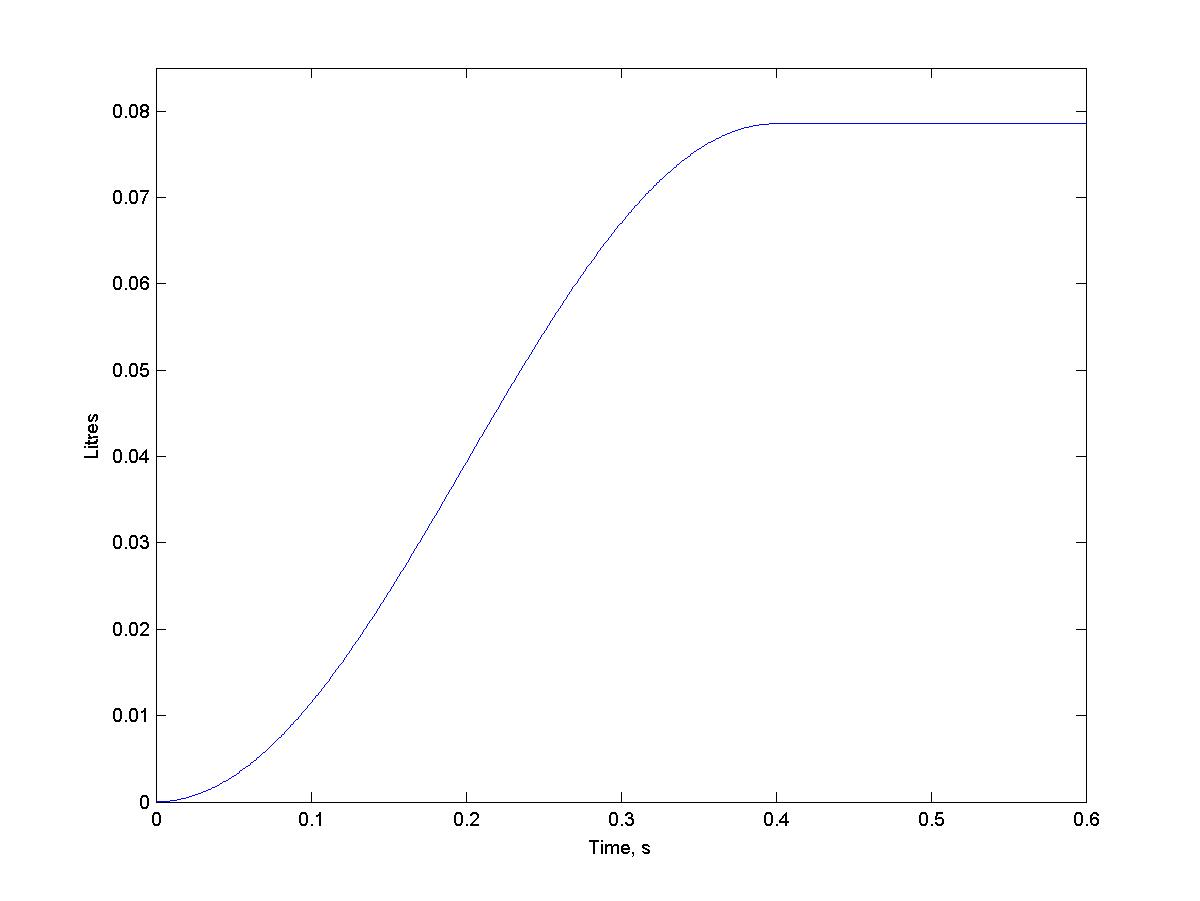
\includegraphics[width=15cm]{motion}
\caption{Contraction curve generated by the function {\tt Motion}.}
\label{fig:contra}
\end{center}
\end{figure}

\begin{figure}[!hb]
\begin{center}
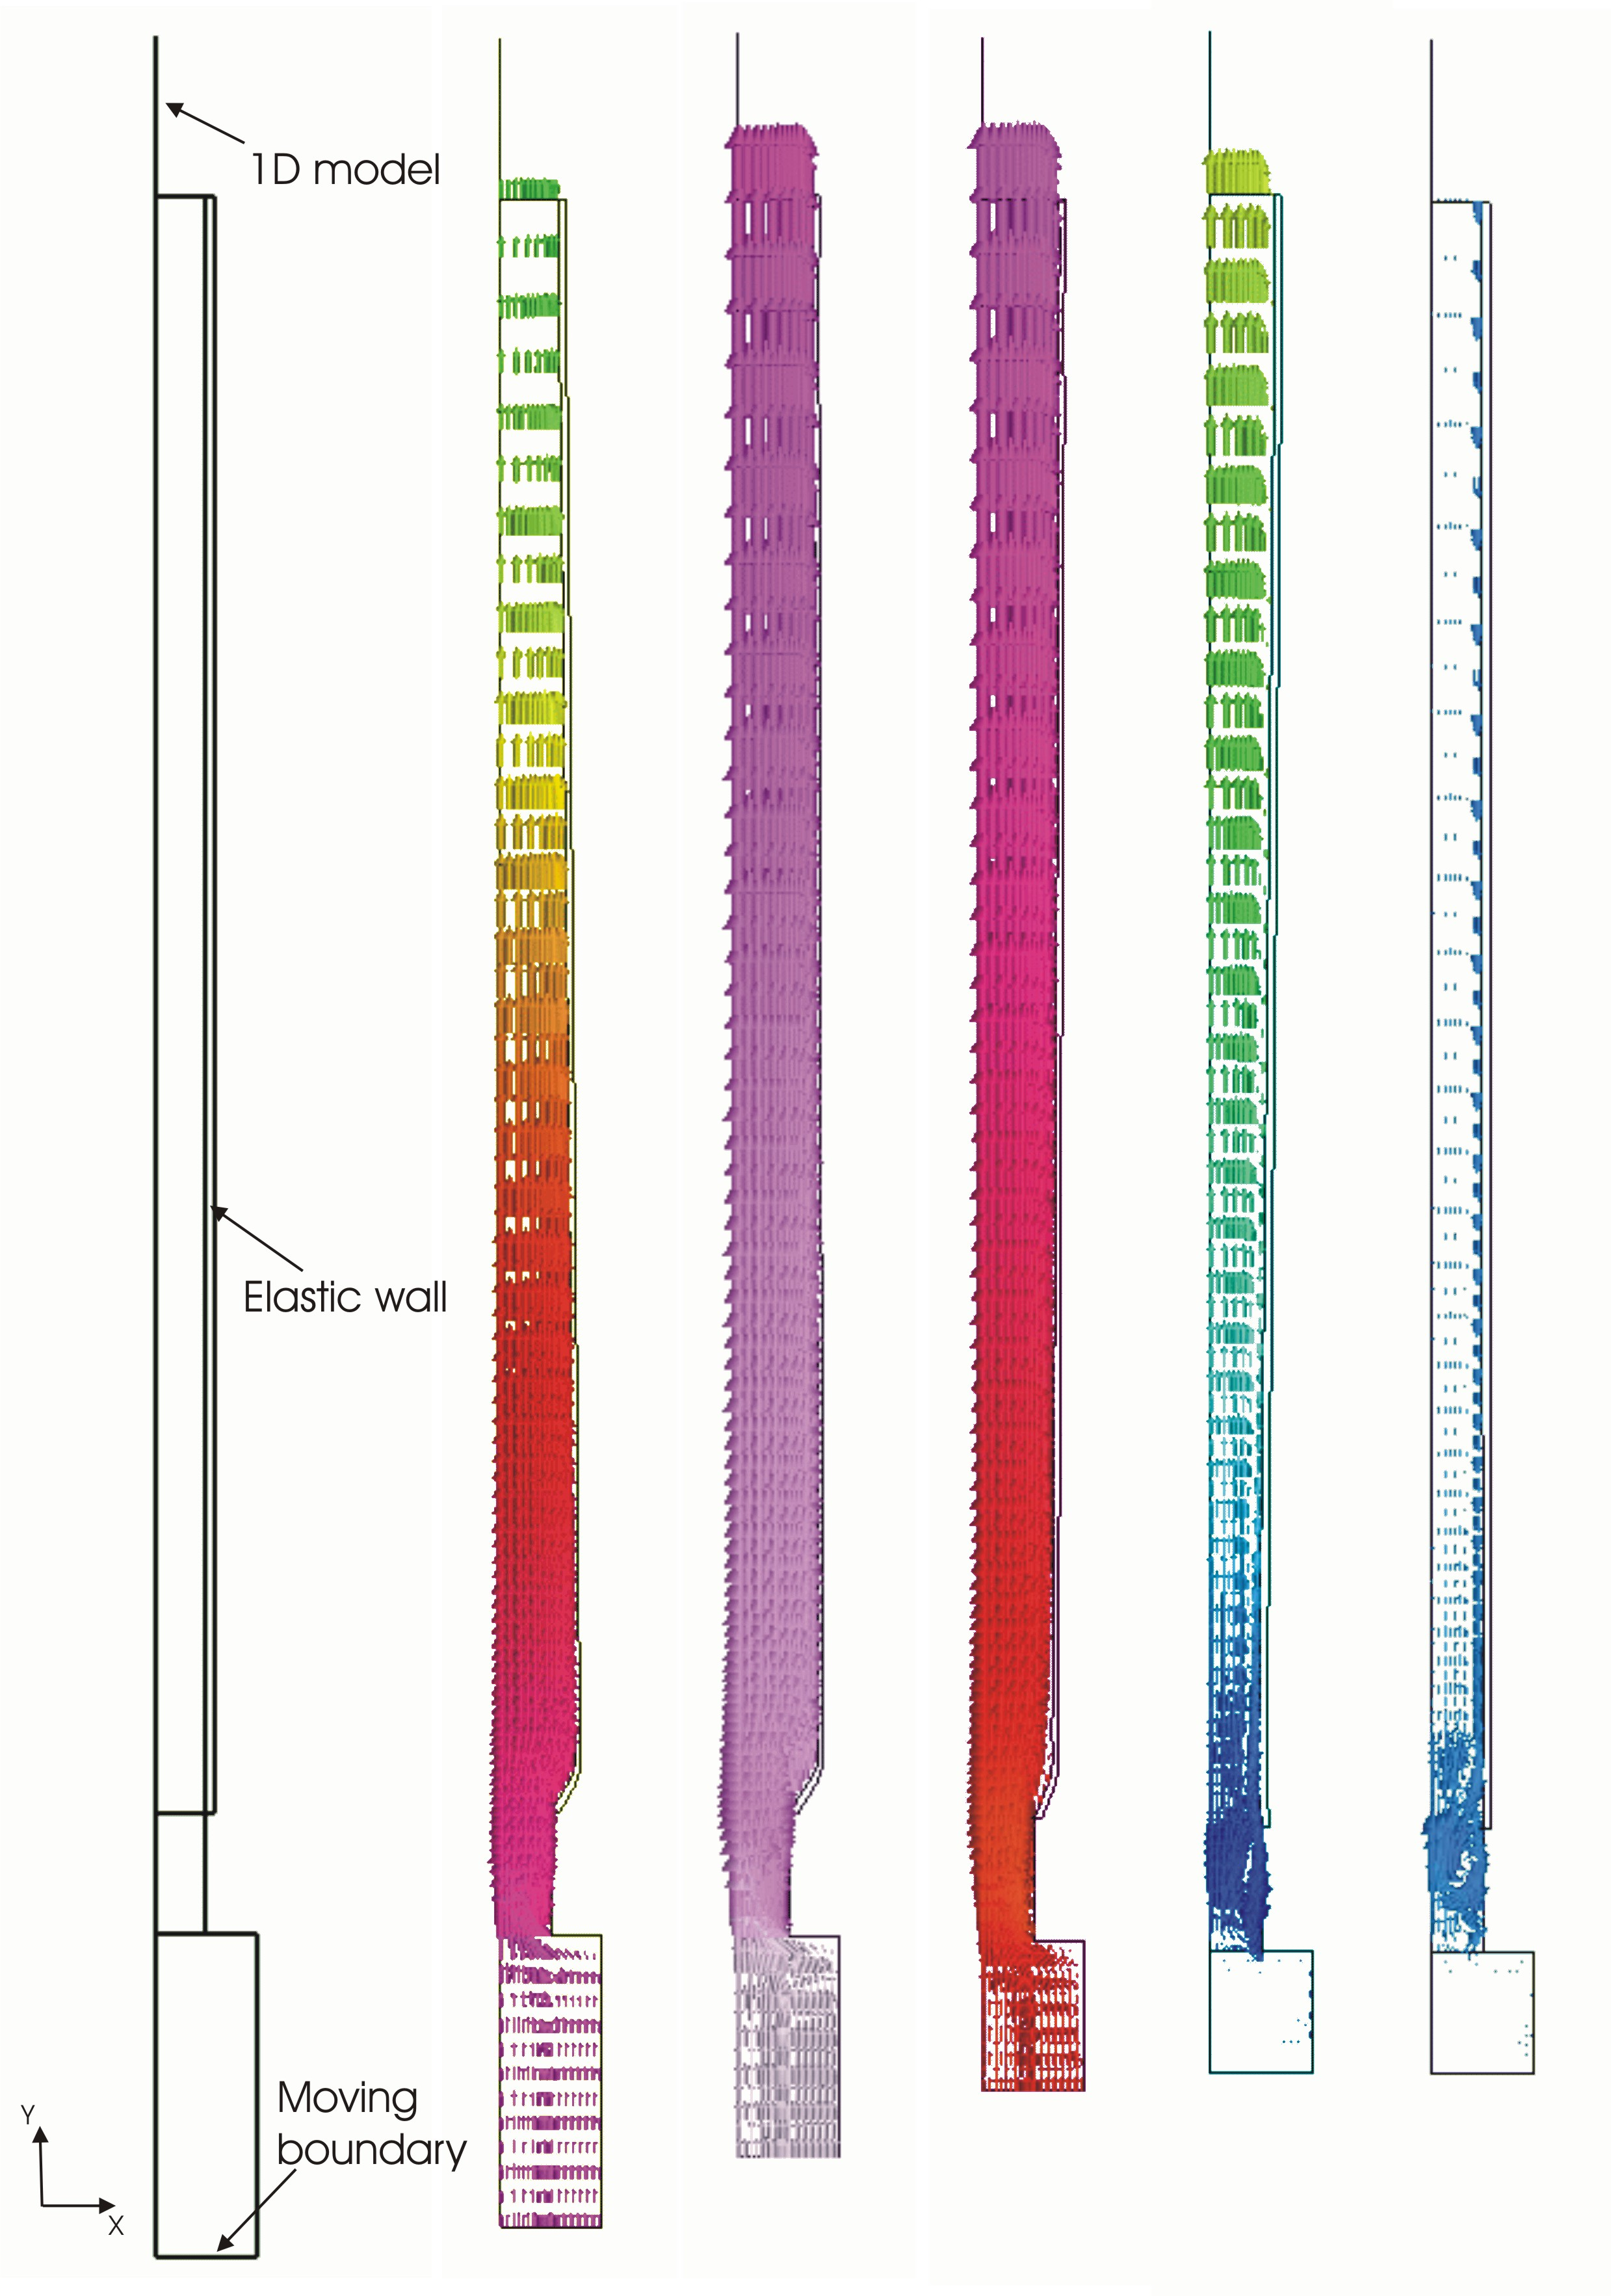
\includegraphics[width=\textwidth]{kollaasi}
\caption{The geometry of the model and velocity fields at 5 time steps, 
100, 200, 300, 400 and 500 ms.  The displacements of the wall are 
magnified by factor of 10.}
\label{fig:velofields}
\end{center}
\end{figure}




\part{Miscallenous Problems}

\graphicspath{{./}{TemperatureOperatorSplitting/}}
\chapter{Operator splitting in the evolutionary heat equation}

\modinfo{Directory}{TemperatureOperatorSplitting}
\modinfo{Solvers}{HeatSolve, TransportEquationSolver, 
RateOfChangeSolver} 
\modinfo{Tools}{Editor} 
\modinfo{Dimensions}{2D, Transient simulation}


\subsection*{Introduction}

The drawback of the stabilized finite element formulations available
in Elmer to solve the convection-diffusion equation and Navier-Stokes
equations is that these methods are computationally expensive, in particular
when the residual-free-bubbles formulation is used.
In evolutionary problems the reduction of computational cost may be attempted
by applying operator splitting techniques in which the original equation at
each time step is splitted up into subproblems that are
easier to solve numerically.

The aim of this chapter is to provide an illustrative example on
using operator splitting capability in the solution of the 
time-dependent heat equation. 
% and Navier-Stokes equations.   
For the theoretical background of the operator splitting scheme applied here
the reader is referred to Elmer Models Manual and references therein.


%\section{Example I: The evolutionary heat equation}

\subsection*{Case description}

The problem considered here is the solution of the time-dependent 
heat equation in the homogeneous L-shaped plate the geometry of which is shown 
in Figure~\ref{fg:struct1}. 
The density of the material is taken to be unity, while the heat 
conductivity $k$ of the material is taken to be a 
parameter with values ranging between 0.05 and 0.01. The plate is
heated by a constant internal heat source magnitude of which equals to unity. 
The convection velocity field is assumed to be constant with the two 
Cartesian components of the velocity vector equaling to unity. 
The boundaries $\Gamma_i$,
$i=1,4,5,6$, are kept at constant temperature $0$, while the boundaries
$\Gamma_2$ and $\Gamma_3$ are assumed to be insulated, i.e.\ the heat flux
on this part of the boundary vanishes. 

The problem is to solve the temperature distribution in the plate. 
The time interval for the simulation is taken to be [0,2] and the temperature 
of the plate is 0 at the time $t=0$. 


\subsection*{Solution procedure}

Using operator splitting the solution of the heat equation may be replaced 
at each time step by the solution of three subproblems consisting of two 
time-dependent Poisson equations and the convective transport problem.
The effects of diffusion and convection are decoupled by this 
splitting so that 
the diffusion and convection phenomena are taken into account by the steps 
involving the solution of the Poisson equation and the convective transport 
problem, respectively. 

The time-dependent Poisson equations can be solved using the basic heat 
equation solver in Elmer. To avoid the use of stabilized finite element 
formulations in the solution of the convective transport problem this 
subproblem is solved by discretizating an equivalent wave-like equation 
formulation (second order in time equation). 
  
When the operator splitting method is applied,
specific care is needed in prescribing boundary and initial conditions
for the simulation. While the boundary conditions (and initial conditions) 
for the steps involving the solution of the Poisson equation may be defined in 
the usual manner, the boundary conditions for the convective 
transport problem may be prescribed
only on the part of inflow boundary on which the temperature is prescribed. 
In the example the inflow boundary is the union of the boundary segments 
$\Gamma_i$, $i=1,2,5,6$,
so the boundary conditions for the convective transport equation 
should be given on $\Gamma_i$, $i=1,5,6$.
In addition to prescribing the boundary conditions, the rate of change of
the field subject to the convection operator (here temperature) is needed as 
an initial condition at the beginning of pure convection step. This field 
can be solved using a specific solver ({\tt RateOfChangeSolver}) prior to
the solution of the convective transport problem. 
The boundary conditions for this 
solver should be prescribed on the same part of the boundary on which the 
boundary conditions for the convective transport problem are prescribed.    

It should be noted that in connection with the operator splitting method
the user should specify an even number of time steps.
Although the details of implementation need not be known in order to use
the operator splitting ability, it is noted that the the running of two 
successive time steps actually constitutes a single operator splitting scheme
step as described in Elmer Models Manual. 
There are thus three equations (referred to as {\tt Heat Equation},
{\tt Rate Of Change Equation} and {\tt Transport Equation}) which may be 
solved at one time step. 
At odd time steps all these equations are solved meaning that
both the diffusion and convection steps are taken, whereas at even time
steps the solution of the convective transport problem is omitted so that
the diffusion step is performed only. Physically meaningful results
satisfying all the essential boundary conditions may thus be written to
the results file only after even time steps.
 
The mesh for this example was created using Femlab and tools for 
converting meshes from Femlab to Elmer format. The mesh in Elmer format is 
given in the tutorial files. This unstructured mesh
consists of 8458 elements each of which having three nodes.    

The Header section of the solver input file is used to declare the directory
containing the Elmer mesh files:

\ttbegin
Header
  Mesh DB "." "femlab-mesh"
End
\ttend

The Simulation section of the solver input file is used to declare the 
coordinate system and simulation type as well as simulation parameters 
related to the time discretization scheme: 

\ttbegin
Simulation
  Coordinate System = String "Cartesian 2D"
  Simulation Type = String "Transient"
  Timestepping Method = String "Crank-Nicolson"
  Timestep Intervals(1) = Integer 200
  Timestep Sizes(1) = Real 0.01
  Output Intervals(1) = Integer 1
  Steady State Max Iterations = Integer 1
  Post File = File "os-example.ep"
End
\ttend

Here the keyword {\tt Timestepping Method} is used to 
define the time discretization scheme that is used in the solution of the 
time-dependent Poisson equations. Note that one should not use 
multi-step methods in connection with the operator splitting method. 
The time discretization scheme that is used
in the solution of the convective transport problem is fixed and need not
be specified. It should be noted also that
the number of time steps should be even. Since the equations
solved at one time step are not coupled and can thus be solved in sequential 
manner, {\tt Steady State Max Iterations} may be taken to be 1.     

The Body section of the solver input file is used to declare integer 
identifiers for body forces, equations, initial conditions and materials: 

\ttbegin
Body 1
  Body Force = Integer 1
  Equation = Integer 1
  Initial Condition = Integer 1
  Material = Integer 1
End
\ttend

The Equation section of the solver input file in turn has the following 
declaration

\ttbegin
Equation 1
  Active Solvers(3) = Integer 1 2 3
End
\ttend
indicating that three equations are to be solved using solvers with 
the integer identifiers 1, 2 and 3.   
Accordingly, three Solver sections are needed.  
The first Solver section is used for the Poisson equation and has the 
following declarations:

\ttbegin
Solver 1
  Equation = String "Heat Equation"
  Variable = String "Temperature"
  Variable Dofs = Integer 1
  Linear System Solver = String "Iterative"
  Linear System Iterative Method = String "BiCGStab"
  Linear System Max Iterations = Integer 350
  Linear System Convergence Tolerance = Real 1.0e-08
  Linear System Abort Not Converged = Logical True
  Linear System Preconditioning = String "ILU0"
  Steady State Convergence Tolerance = Real 1.0e-05
  Stabilize = Logical False
  Bubbles = Logical False
End
\ttend
Note that there is no need to use stabilization, so the values of the keywords 
{\tt Stabilize} and {\tt Bubbles} may be set to be {\tt False} to reduce the
computational cost. 

The remaining two Solver sections are related to the convective transport
problem. The first one of these sections is used to declare the solver
parameters related to the problem ({\tt Rate Of Change Equation}) the 
solution of which gives the approximation to the rate of change of the 
temperature at the beginning of pure convection step. The contents
of this solver section is 

\ttbegin
Solver 2
  Equation = String "Rate Of Change Equation"
  Procedure = File "RateOfChange" "RateOfChangeSolver"
  Variable = String "Udot0"
  Variable Dofs = Integer 1   
  Advection = String "Constant"
  Advection Variable = String "Temperature" 
  Linear System Solver = String "Iterative"
  Linear System Iterative Method = String "BiCGStab"
  Linear System Max Iterations = Integer 350
  Linear System Convergence Tolerance = Real 1.0e-08
  Linear System Abort Not Converged = Logical True
  Linear System Preconditioning = String "ILU0"
  Steady State Convergence Tolerance = Real 1.0e-05
End
\ttend

Here the keyword {\tt Advection Variable} is used to declare the quantity
which is subject to the convection operator, while the keyword {\tt Advection}
is used to define the type of the velocity vector.
The name {\tt Udot0} is used for the solution of this problem.

Finally, the Solver section for the wave-like equation, which is equivalent to 
the convective transport equation, has the following declarations:

\ttbegin
Solver 3  
  Equation = String "Transport Equation"
  Procedure = File "TransportEquation" "TransportEquationSolver"
  Time Derivative Order = Integer 2
  Variable = String "U"
  Variable Dofs = Integer 1  
  Advection = String "Constant"
  Advection Variable = String "Temperature" 
  Rate Of Change Equation Variable = String "Udot0" 
  Linear System Solver = String "Iterative"
  Linear System Iterative Method = String "BiCGStab"
  Linear System Max Iterations = Integer 350
  Linear System Convergence Tolerance = Real 1.0e-8
  Linear System Abort Not Converged = Logical True
  Linear System Preconditioning = String "ILU0"
  Steady State Convergence Tolerance = Real 1.0e-05
End
\ttend

The name {\tt U} is used for the solution of the convective transport problem. 
The value of the keyword {\tt Time Derivative Order} must be 2.
The use of the keywords {\tt Advection Variable} and {\tt Advection}
is similar to that explained in connection with the second solver section.  

The Material section is used to declare the material properties and,
as the velocity vector in the convection operator is of constant type,
also the components of the velocity vector. In the case $k=0.01$ the contents 
of this section is  

\ttbegin
Material 1
  Density = Real 1
  Heat Capacity = Real 1
  Heat Conductivity = Real 0.01
  Advection Velocity 1 = Real 1
  Advection Velocity 2 = Real 1
End
\ttend

Body Force section is used to declare the body force in the Poisson
equations.

\ttbegin
Body Force 1
  Heat Source = Real 1
End
\ttend

Finally, the initial conditions and boundary conditions are specified. 
The temperature at $t=0$ is defined by giving the declaration  

\ttbegin
Initial Condition 1
  Temperature = Real 0
End
\ttend

Two Boundary Condition sections are needed. The first one is used 
to prescribe the boundary conditions on the part of inflow boundary where
the temperature is given: 

\ttbegin
Boundary Condition 1
  Target Boundaries(3) = Integer 1 2 4 
  Temperature = Real 0
  Udot0 1 = Real 0
  U 1 = Real 0
End
\ttend

The rate of change of the temperature is zero on this part of the boundary 
as the temperature is kept fixed. Thus the zero boundary 
conditions for {\tt Udot0} are defined. The boundary value of the 
solution to the convective transport problem should equal to the
temperature. Therefore zero boundary conditions for {\tt U} are also defined.
  
The second Boundary Condition section is used to define the Dirichlet boundary 
conditions on the outflow boundary: 

\ttbegin
Boundary Condition 2
  Target Boundaries(1) = Integer 3
  Temperature = Real 0
End
\ttend

Note that the zero heat flux condition
need not be specified explicitly. Similarly, the treatment of 
the outflow boundary conditions for the wave-like
equation are handled automatically by the code and need not be specified. 


\subsection*{Results}

From a numerical point of view the solution of the problem becomes 
increasingly difficult as the heat conductivity $k$ tends to zero. 
In order to examine possible dependence on the heat conductivity parameter
the problem was solved in three cases with $k$ taking values 0.05, 0.025 
and 0.01. For comparison the same case was solved using three alternative 
methods. Here the operator splitting scheme is referred to as OS, S is the 
stabilized finite element method and RFB is the method based on the 
residual-free-bubbles formulation. In the case of methods S and RFB the 
simulation was performed using 100 time steps which corresponds to the number 
of 200 time steps used in the case of operator splitting scheme.
 
The maximum temperature at $t=2.0$ is recorded in 
Table~\ref{methodvstemperature}. The CPU time used in the simulation to
obtain solution for a certain value of the heat conductivity is
shown in Table~\ref{methodvscpu}.
   
\begin{table}  
\caption{The maximum temperature at $t=2.0$. For comparison 
the maximum temperature according to the steady state solution is also 
recorded.}
\label{methodvstemperature}
\begin{center}
\begin{tabular}{lccc}\hline
Method            &        &  $k$   &                \\ \hline
                  & 0.05   & 0.025  & 0.01           \\ \hline
OS                & 1.0235 & 1.0424 & 1.0677         \\
S                 & 1.0269 & 1.0436 & 1.0418         \\
S(steady state)   & 1.0279 & 1.0437 & 1.0418         \\
RFB               & 1.0271 & 1.0458 & 1.0853         \\
RFB(steady state) & 1.0286 & 1.0462 & 1.1050         \\ \hline
\end{tabular}
\end{center}
\end{table}

\begin{table} 
\caption{CPU time used by the different methods for simulation ($k=0.01$).}
\label{methodvscpu}
\begin{center}
\begin{tabular}{lc}\hline
Method            & CPU     \\ \hline
OS                & 211.13  \\
S                 & 82.16   \\
RFB               & 340.70  \\ \hline
\end{tabular}
\end{center}
\end{table}


\subsection*{Discussion}

The benefit of the wave-like equation formulation of the convective 
transport problem is that this formulation can be discretizated without
using stabilized finite element formulations. Thus all the subproblems
arising from operator splitting can be solved using standard FE
techniques. On the other hand,
the expense of this approach is that one is lead to handle the second
order in time equation. 

In the current implementation of the method the 
wave-like equation is discretizated in time
using the Crank-Nicolson scheme which is expected to perform well if 
the solution to the convective transport problem is smooth. Spurious
oscillations may however occur in the case of a rough solution changing 
rapidly in short length scales. The user of the method should be
aware that the deterioration of accuracy may thus occur if the solution is
not smooth and $\epsilon=k/||\vec u ||_\infty \longrightarrow 0$,
meaning that convection dominates.  
   
In the cases considered convection dominates, the parameter $\epsilon$ 
ranging between $3.5\cdot 10^{-2}$ and $7.1\cdot 10^{-3}$,
and the solution has also sharp boundary 
layer near the upper edge. No spurious oscillations are however detected in
the solution. Nevertheless, the results recorded in 
Table~\ref{methodvstemperature} indicate that the differences between the
methods become larger as $\epsilon \longrightarrow 0$. 
 
In view of the results shown in Table~\ref{methodvscpu} the accuracy of the 
operator splitting scheme in predicting the maximum temperature is comparable 
to that of the residual-free-bubbles method while the computational 
cost measured in CPU time is reduced by approximately 40~\% when 
the operator splitting scheme is used. 

It should be noted that the operator splitting scheme has 
the favourable feature that small spurious oscillations present in the 
solution after pure convection step may naturally be damped by the step 
involving diffusion phenomena. Note also that each of the subproblems arising 
from the operator splitting may be
solved very efficiently using multigrid techniques, whereas robust multigrid 
solvers amenable to solving linear systems arising from direct discretization 
of the convection-diffusion equation are still to be found. This makes 
the operator splitting scheme attractive in the solution of problems 
having a very large number of unknowns.   




%\section{Example II: The evolutionary Navier-Stokes equations}





\graphicspath{{./}{PoissonBEM/}}
\chapter{Temperature distribution with BEM}

\modinfo{Directory}{PoissonBEM}
\modinfo{Solvers}{\Idx{PoissonBEMSolver}}
\modinfo{Tools}{\Idx{ElmerGrid}, editor}
\modinfo{Dimensions}{2D}

\subsection*{Case definition}
This tutorial uses boundary element method (\Idx{BEM}) to solve Poisson equation.
Even though Elmer is primarily a finite element software the are limited
support also for BEM computation. One should however note that Elmer does not
include any multilevel strategies essential for a good performance.
For more details about BEM check the Elmer Models Manual.
The simulation setting is described in Figure~\ref{f:simulationSetting}. 
A heater with constant heat flux is placed inside a box and the walls of the box are in 
fixed temperature.
We are interested in the temperature distribution in the medium around the heater ($\Omega$)
and on the surface of the heater ($\Gamma_1$). We also want to know the heat flux through the
walls of the box ($\Gamma_2$).
\begin{figure}[!htb]
\begin{center}
\setlength{\unitlength}{0.17cm}
\begin{picture}(30,30)
% box walls  *****************
\put(0,0){\line(1,0){30}}
\put(0,30){\line(1,0){30}}
\put(0,0){\line(0,1){30}}
\put(30,0){\line(0,1){30}}
% heater walls ***************
\put(10,10){\line(1,0){10}}
\put(10,20){\line(1,0){10}}
\put(10,10){\line(0,1){10}}
\put(20,10){\line(0,1){10}}
% some text ******************
\put(11,25){$\Omega$, medium}
\put(12.5,14.5){heater}
\put(10,7.5){$\Gamma_1$, $-\frac{\partial T}{\partial n} = 1$}
\put(11,1){$\Gamma_2$, $T=0$}
\end{picture}
\end{center}
\caption{Simulation setting}
\label{f:simulationSetting}
\end{figure}

\subsection*{Solution Procedure}
First we create a mesh with ElmerGrid. The mesh is defined in
{\tt heater.grd} and it is created with command
\ttbegin
ElmerGrid 1 2 heater
\ttend
The solver input file {\tt PoissonBEM.sif} starts with 
the definition of the mesh directory. 
\ttbegin
Header
  Mesh DB "." "heater"
End
\ttend
The simulation uses 2D cartesian geometry, searches a steady state and since
there is no coupled solvers only one iteration is needed.
Numerical results are written to file {\tt BEM\_Temperature.result}
and ElmerPost file is {\tt BEM\_Temperature.ep}.
\ttbegin
Simulation
  Coordinate System =  Cartesian 2D
  Coordinate Mapping(3) = 1 2 3

  Simulation Type = Steady
  Steady State Max Iterations = 1

  Output Intervals = 1
  Post File = "BEM_Temperature.ep"
  Output File = "BEM_Temperature.result"
End
\ttend
There is just one body, the medium around the heater, and it uses equation 1.
\ttbegin
Body 1
  Name = "medium"
  Equation = 1
End
\ttend
In equation block we say that we use the solver named {\tt PoissonBEM}.
\ttbegin
Equation 1
  PoissonBEM = Logical True
End
\ttend
In solver block the {\tt Equation} keyword must match the one in equation block.
We also need to define the procedure, name the variable ({\tt Temperature}) and tell 
the degrees of freedom of the variable. Keyword {\tt Optimize Bandwidth} must be set to false
with BEM solver. Since we were interested in the flux, we must now export it to the
results. The lines beginning {\tt Exported} must be exactly as below. Keywords beginning
{\tt Linear System} can be used except that the preconditioning cannot be ILU.
\ttbegin
Solver 1
  Equation = PoissonBEM
  Procedure = "PoissonBEM" "PoissonBEMSolver"
  Variable = Temperature
  Variable DOFs = 1

  Optimize Bandwidth = False

  Exported Variable 1 = String Flux
  Exported Variable 1 DOFs = 1

  Linear System Solver = Iterative
  Linear System Iterative Method = BiCGStab
  Linear System Preconditioning = Jacobi
  Linear System Max Iterations = 100
  Linear System Convergence Tolerance = 1.0e-8

  Steady State Convergence Tolerance = 1.0e-6
End
\ttend
Finally we give the boundary conditions for the heater surface and for the walls of the 
box. The keyword {\tt Body Id} tells the reference body of this boundary. Here it is 1. 
The keyword {\tt Normal Target Body} tells the direction of the outer normal. Value -1 
means the side where there are no volume elements. We didn't mesh the inside of 
the heater and so we can use value -1 in both cases. The heat flux from heater to
medium is 1 and the walls of the box are set to zero temperature. The keyword
{\tt Temperature} matches the name of the variable in solver block.
\ttbegin
Boundary Condition 1
  Name = "heater_surface"
  Target Boundaries = 1

  Body Id = 1
  Normal Target Body = Integer -1
  Flux = Real 1
End

Boundary Condition 2
  Name = "box_walls"
  Target Boundaries = 2

  Body Id = 1
  Normal Target Body = Integer -1
  Temperature = 0
End
\ttend
\subsection*{Results}
Problem is solved with command {\tt Solver}. The results are then viewed with
{\tt ElmerPost}. In Figure~\ref{f:temperature} is the temperature distribution.
\begin{figure}[!hb]
\begin{center}
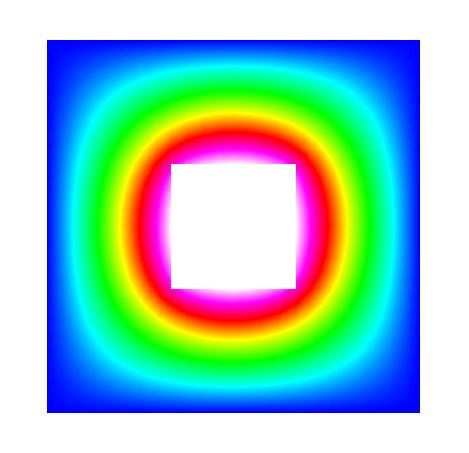
\includegraphics[width=0.4\textwidth]{temperature}
\end{center}
\caption{The temperature distribution.}
\label{f:temperature}
\end{figure}





















\graphicspath{{./}{Temperature1D/}}
\chapter{Adding user defined equation solver}

\modinfo{Solvers}{\Idx{PoissonSolver}} 
%\modinfo{Files}{1dheat.grd, 1dheat.sif, Poisson.f90}
\modinfo{Tools}{Editor, \Idx{Fortran 90 compiler}, \Idx{ElmerGrid}}
\modinfo{Dimensions}{1D, Steady-state}

\subsection*{Problem description}

This tutorial is about creating the code for a simple poisson equation solver.
The solver is applied to 1d case with internal source term and fixed boundaries.

Mathematically the problem we solve is
\begin{equation}
\left \{
\begin{array}{cccc}
- \Delta \Phi &= &f & \mbox{ in } \Omega \\
\Phi&=&0 & \mbox{ on } \Gamma
\end{array}
\right .
\end{equation}

Allthough this example is in 1d the same solver code also applies to 2D and 3D
problems.

\subsection*{Solution procedure}

Own codes solving some specific equation may be added dynamically to Elmer 
software. Here we create a very simple equation solver code. The final code
may be found in the tutorial directory as well as the files for running
the example. The solution may be attempted as follows:

\begin{itemize}
\item Copy all the files from tutorial directory to current directory
\item Setup Elmer
\item Give the following commands:
\ttbegin
elmerf90 -o Poisson Poisson.f90
ElmerGrid 1 2 1dheat
ElmerSolver
ElmerPost
\ttend
\end{itemize}

\subsection*{The solver code}

The example Fortran code may be found in the tutorial files under the
name Poisson.f90.  The example run is defined in 1dheat.sif.
Only a rough guidline is given here of both of the files, refer to the
files themselves for more details.

All the  equation solvers in Elmer have the following common interface
\ttbegin
SUBROUTINE PoissonSolver( Model, Solver, dt, TransientSimulation )
  USE SolverUtils

  TYPE(Model) :: Model
  TYPE(Solver_t), POINTER :: Solver
  REAL(KIND=dp) :: dt
  LOGICAL :: TransientSimulation

    ...
END SUBROUTINE PoissonSolver
\ttend

The argument Model contains pointers to the whole definition of the Elmer run.
The argument Solver contains parameters specific to our equation solver.
The argument dt and TransientSimulation are the current timestep size, and a
flag if this run is steady or transient. These don't concern us this time.

When starting the ElmerSolver looks the solver input (.sif) file for a
Solver section with keyword "Procedure". This should contain reference to
the compiled code

\ttbegin
   Procedure = "Poisson" "PoissonSolver"
\ttend
where the first string in the right hand side is the file name of the compiled
code, and second argument is the name of the subroutine to look for in the given file.

In the Solver section one also gives the name of the field variable
(here Poisson) and the DOFs/node (here 1).

The basic duty of the equation solver is to solve one or more field variables inside
the time progressing- or steady state iteration-loop of ElmerSolver.  Here we use
FEM to discretize the Poisson equation and finally solve the equation by calling
ElmerSolver utility SolveSystem.

The solution progresses the following way:

\begin{itemize}
\item Get the space for variables and temporaries from ElmerSolver and compiler.
The matrix structure and space for solution and RHS vector have already been
allocated for you before you enter the equation solver.

The matrix is of type Matrix\_t and may be obtained from the arguments as
\ttbegin
TYPE(Matrix_t), POINTER :: StiffMatrix
StiffMatrix => Solver % Matrix
\ttend
Usually one doesn't need to know the internal storage scheme or the fields
of the Matrix type, but one just passes this pointer further to ElmerSolver
utility routines.

Similarly, the force vector may be accessed as follows:
\ttbegin
REAL(KIND=dp), POINTER :: ForceVector(:)
ForceVector => StiffMatrix % RHS
\ttend

The solution vector is obtainable similarily
\ttbegin
TYPE(Variable_t), POINTER :: Solution
Solution => Solver % Variable
\ttend

The Variable\_t structure contains the following fields
\begin{itemize}
\item DOFs: the number of degrees of freedom for one node. This value is for
information only and should'nt be modified.
\item Perm: an integer array that is nonzero for nodes that belong
to computational volume for this equation. The entry $Perm(i)$ holds
the index of the global matrix row  (for 1 DOF) for nodal point i.
This array  should'nt be modified by the equation solver.
\item Values: Space for the solution vector values.
Note that the values
are ordered the same way as the matrix rows, .i.e. the value of Potential at node
n is stored at
\ttbegin
  val = Solution % Values( Solution % Perm(n) )
\ttend
\end{itemize}


\item Initialize the global system to zero. Calling the utility routing
\ttbegin
CALL InitializeToZero( StiffMatrix, ForceVector )
\ttend
is usually enough.


\item Go trough the elements for which this equation is to 
be solved, get the elemental matrices and vectors and add them to
the global system:

\ttbegin
DO i=1,Solver % NumberOfActiveElements
   CurrentElement => Solver % Mesh % Elements( Solver % ActiveElements(i) )
      ...
   CALL LocalMatrix( ... )
   CALL UpdateGlobalEquations( ... )
END DO
CALL FinishAssembly( ... )
\ttend

Here the LocalMatrix is your own subroutine computing elemental matrices and vectors.
In the example code LocalMatrix uses three routines from ElmerSolver utilities. The function 
\ttbegin
  dim = CoordinateSystemDimension()
\ttend
returns the dimension of the current coordinate system, i.e. the return value is 
1, 2 or 3 depending on the input file setting of keyword "Coordinate System". The function
GaussPoints returns structure containing the integration point local coordinates and weights
\ttbegin
  TYPE(GaussIntegrationPoints_t) :: IntegStuff
  IntegStuff = GaussPoints( Element )
\ttend
The fields of the type GaussIntegrationPoints\_t are
\ttbegin
INTEGER :: n
REAL(KIND=dp) :: u(:), v(:), w(:), s(:)
\ttend
the integer value n is the number of points selected. The arrays u,v and w
are the local coordinates of the points, and the array s contains the weights
of the points. One may call the GaussPoints-routine with second argument,
\ttbegin
  IntegStuff = GaussPoints( Element, n )
\ttend
if the default number of integration points for given element is not suitable.

Inside the integration loop the function ElementInfo is called:
\ttbegin
   TYPE(Element_t), POINTER :: Element
   TYPE(Nodes_t) :: Nodes
   REAL(KIND=dp) :: U,V,W,detJ, Basis(n), dBasisdx(n,3), ddBasisddx(n,3,3)

   stat = ElementInfo( Element, Nodes, U, V, W, detJ,  &
        Basis, dBasisdx, ddBasisddx, .FALSE. )
\ttend
This routine returns determinant of the element jacobian (detJ), basis function values
(Basis(n)), basis function global derivative values (dBasisdx(n,3)), basis function second
derivative values ( ddBasisddx(n,3,3) ). The second derivatives are only computed if the
next logical flag is set to true. All the values are computed at the point U,V,W inside
element defined by structures Element and Nodes.

Refer to the code for more details.

\item Set boundary conditions. Here only dirichlet boundary conditions are used. These
may be set by using the utility routine SetDirichletBoundaries.

\item Solve the system by calling utility routine SolveSystem.
\end{itemize}


\begin{figure}
\begin{center}
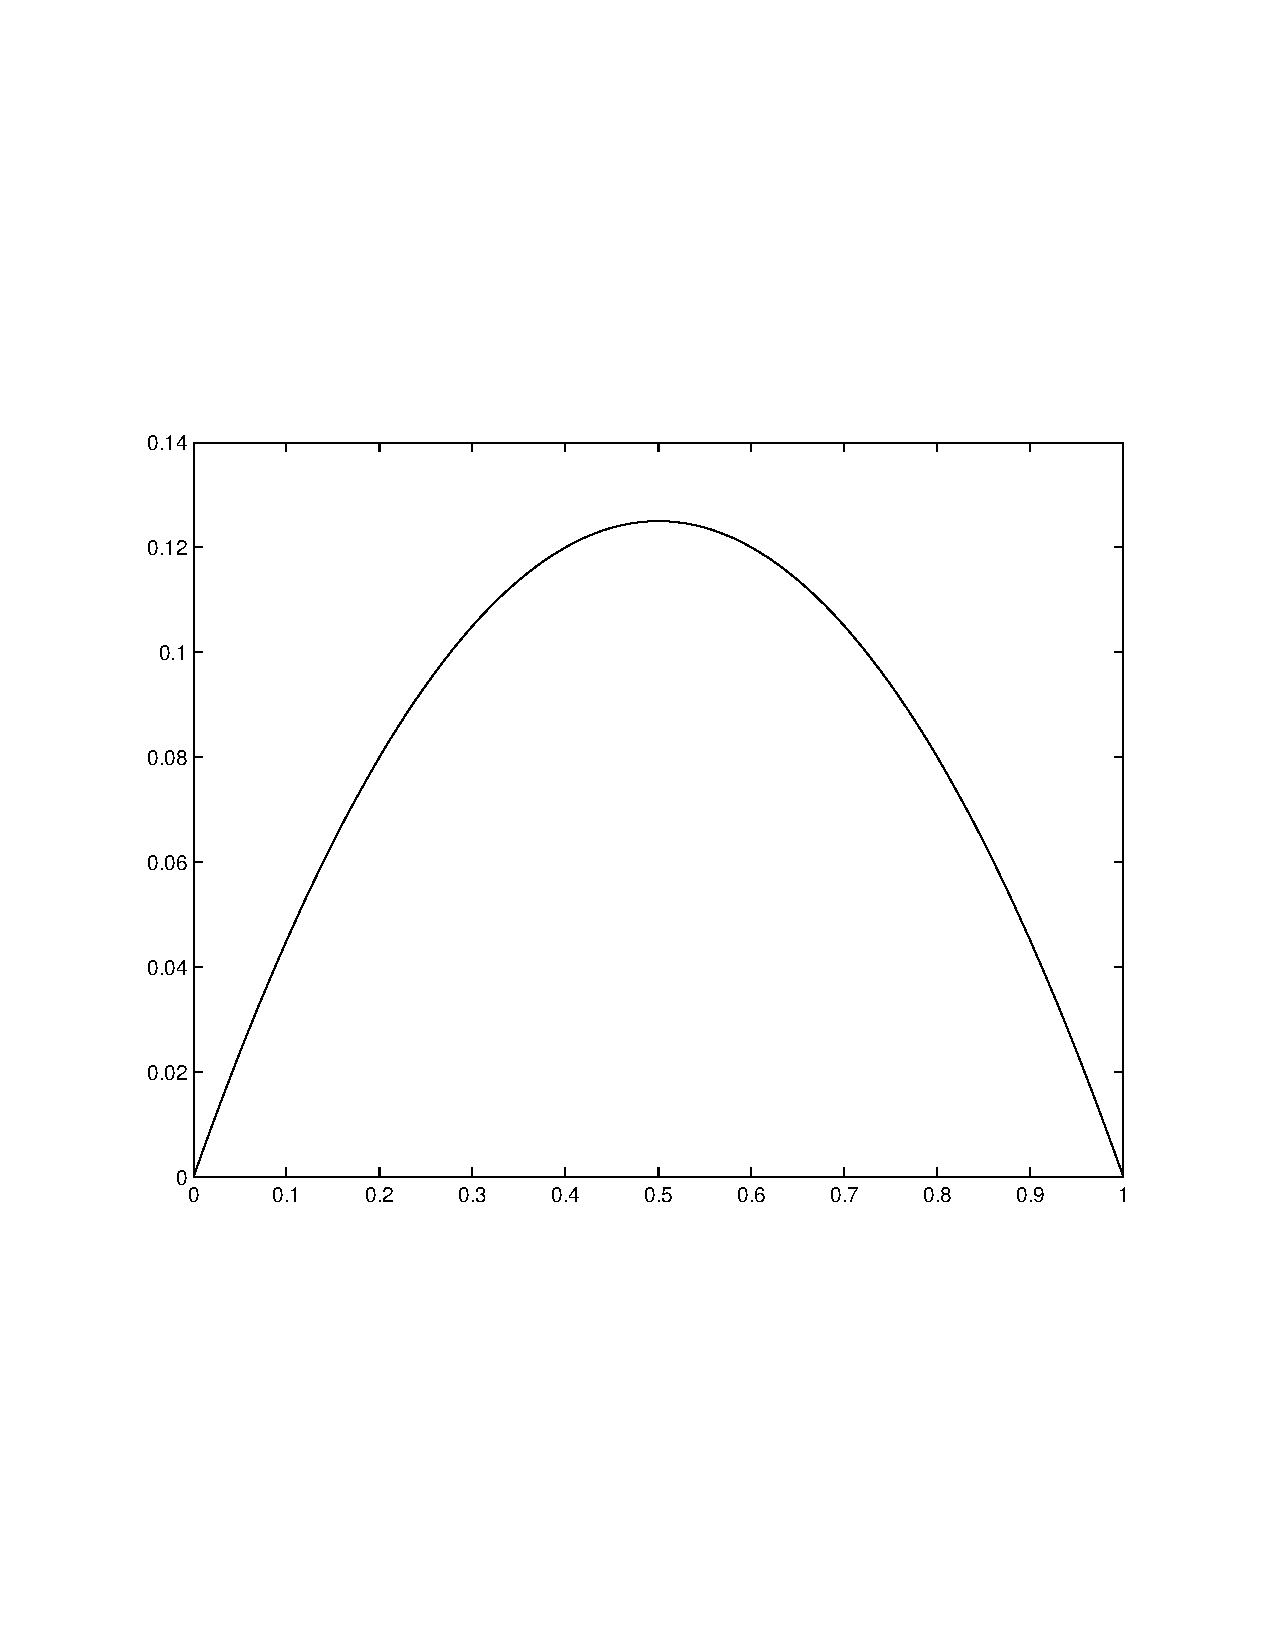
\includegraphics[width=0.6\textwidth]{1dheat}
\caption{Solution of the Poisson Equation.}\label{fg:pot}
\end{center}
\end{figure}
\subsection*{Results}

In the elmerpost file there is a variable called Potential which contains the
solution of this simple example. See figure~\ref{fg:pot}


\graphicspath{{./}{FlowLinearRestriction/}}
\chapter{\Idx{Linear Constraints}}
\noindent
\modinfo{Module name}{included in solver (SolverUtils)}
\modinfo{Module subroutines}{\Idx{SolveWithLinearRestriction}}
\modinfo{Module authors}{Mika Juntunen}
\modinfo{Document authors}{Mika Juntunen}
\modinfo{Document edited}{August 5th 2003}

\section{Introduction}
This subroutine allows user to solve problems with linear constraints.
Here constraints are forced with \Idx{Lagrange multipliers}. This method,
however, does not always lead to a well-posed problem. Conditions that ensure
a (unique) solution are excluded here, but the conditions are found in many
books (check for example~\cite{c:girault}).  

\section{Theory}
The problem at hand is
\begin{equation}\label{e:problem}
\min_x \, x^T A x - x^T f
\end{equation}
Let's assume that we can solve this. Now we also want that the solution
solves the system $Bx = g$. This gives constraints to our solution.
The rank of $B$ should be less or equal to the rank of $A$.
Loosely speaking, the number of rows in $B$ should be less or equal to the
number of rows in $A$. The method of Lagrange multipliers fixes these two
equations together and gives a new functional to minimize.
\begin{equation}
\min_x \, x^T A x - x^T f +\lambda^T ( Bx-g )
\end{equation}
If $A$ is symmetric, then simple variational approach leads to solving
$x$ out of system
\begin{equation}
\begin{pmatrix}
A & B^T \\
B & 0 
\end{pmatrix} 
\begin{pmatrix}
x \\
\lambda
\end{pmatrix}
=
\begin{pmatrix}
f \\
g
\end{pmatrix}
\end{equation}
Symmetry of $A$ is not always needed, but then more powerful methods have to be used
to get to the above system.

\section{Limitations}
\begin{itemize}
\item \textbf{General usage of the subroutine} \newline
This subroutine can not be used by just adding keywords to solver input file.
You must somehow create the constraint matrix and then call for SolveWithLinearRestriction
in your own subroutine or function. The reader is encouraged to check for details
in ElmerTutorials.

\item \textbf{EMatrix-field} \newline
The EMatrix-field of the solved system matrix is used passing constraint matrix to
SolveWithLinearRestriction. This will be a problem if some other function or subroutine
tries to use the EMatrix-field. EMatrix-field of the constraint-matrix is internally
used by SolveWithLinearRestriction and should therefor be left alone.

\item \textbf{Exported Multipliers} \newline
The length of the vector that holds the multipliers is limited to be a multiply
of the number of nodes in mesh. This means that the vector usually has extra entries.
These entries are set to zero. This leads to problems in extracting the correct 
values from the result file. Also post processing with ElmerPost is at least tricky.

\item Parallel solving is not yet implemented.

\end{itemize}

\section{Keywords}

\sifbegin
  \sifitemnt{Solver}{solver-id}
  \sifbegin
    \sifitem{Export Lagrange Multiplier}{Logical}
    If the multiplier has some physical meaning, you can save it to result file
    and to post file. This feature has certain drawbacks, check subsection Limitations.
    Default is {\tt False}.

    \sifitem{Lagrange Multiplier Name}{String}
    The name you want to call the exported multipliers. This keyword has no meaning if
    the previous keyword is set to {\tt False}. Default name is 
{\tt LagrangeMultiplier}.
  \sifend
\sifend

\bibliography{elmerbib}
\bibliographystyle{plain}




\graphicspath{{./}{FlowStreamlines/}}
\chapter{\Idx{Streamlines}}
\noindent
\modinfo{Module name}{\Idx{StreamSolver}}
\modinfo{Module subroutines}{StreamSolver}
\begin{versiona}
\modinfo{Module authors}{Mika Juntunen}
\modinfo{Document authors}{Mika Juntunen}
\modinfo{Document edited}{July 30th 2003}

\section{Introduction}

Streamline is a line in flow whose tangent is parallel to velocity field
$\vec u$ of the flow in every point $\vec x$. It should be noted that the path of 
material is generally not the same as streamlines. There is also third set
of closely related lines, namely streak lines. On certain streak line
lie all those flow elements that at some earlier instant passed through
certain point in domain. Of course, the streak lines are generally different
than streamlines but when the flow is steady all three set of lines coincide.

Streamlines are mainly used in providing a picture of the flow field. 
Drawing streamlines so that neighbouring streamlines differ by the same amount, 
gives a picture where direction and magnitude change of flow are clearly prescribed.

\section{Theory}

We are restricted here to the incompressible, steady flow in 2D geometry.
The geometry may be 3D, but it must effectively be 2D as in axis symmetric
geometry.

In 2D cartesian geometry stream function $\psi$ is defined
\begin{equation}\label{e:def2d}
u \, = \, \frac{\partial \psi}{\partial y} \, , \quad
v \, = \, - \frac{\partial \psi}{\partial x} \,.
\end{equation}
Here the geometry is $(x,y)$ and the corresponding flow is $\vec u = (u,v)$.
Let $\Omega$ be the domain of the flow and $\vec v$ a test function for the flow.
Definition~\eqref{e:def2d} leads to finite element approximation
\begin{equation}\label{e:fem2D}
\int_\Omega \nabla \psi \cdot \vec v \, \text{d}\Omega
=
\int_\Omega \vec u^\perp \cdot \vec v \, \text{d}\Omega
\end{equation}

In axis symmetric geometry the mass conservation calculated in a diffenrent way.
This leads to following definition for stream function. 
\begin{equation}\label{e:def_axis}
u \, = \, \frac{1}{r}\frac{\partial \psi}{\partial r} \, , \quad
v \, = \, - \frac{1}{r}\frac{\partial \psi}{\partial z} \,
\end{equation}
where the cylinderical coordinates are $(z,r,\phi)$, velocity components
are $(u,v,w)$ and axis of symmetry is $z$ i.e. $r=0$.
This function is sometimes called the \emph{\Idx{Stokes stream function}} 
and it is not as informative as the stream function in cartesian case.
Of course the finite element approximation is a bit different.
\begin{equation}
\int_\Omega \nabla \psi \cdot \vec v \, \text{d}\Omega
=
\int_\Omega \vec u^\perp \cdot \vec v r \, \text{d}\Omega
\end{equation}
Here the $\phi$ component of the flow is excluded.

From definitions~\eqref{e:def2d} and~\eqref{e:def_axis} it is apparent that 
stream function is constant along the streamlines. So drawing the contours 
of stream function gives the streamlines.

\section{Limitations}

Some limitations of the current implementation:
\begin{itemize}

\item The flow field is asumed to be incompressible.

\item There is no dependency on time. Solver can be used in transient cases, but
it only produces the streamlines of the current flow field as if it was steady. 

\item Only 2D cartesian and axis symetric coordinate systems are implemented.

\item Solver gets the velocity field from user defined variable. In cartesian case
it assumes that first degree of freedom is the $x$-component and the second is the
$y$-component of the velocity. In axis symmetric case it assumes that the first
degree of freedom is the $r$-component and the second is the $z$-component of
the velocity field.

\item User can define the node whose value is first set to zero. This \emph{shouldn't}
have affect on results if the normal stream function is used in cartesian coordinates
and Stokes stream function in axis symmetric coordinates. However, if used stream function
is forced to something else, the position of the first node usually has a large
effect on results. 
This is because the mass conservation is calculated differently.

\end{itemize}


\section{Keywords}
\end{versiona}


\sifbegin
  \sifitemnt{Simulation}{}
  \sifbegin
    \sifitem{Coordinate System}{String} 
    The coordinate system should be set to be one of the following options:
    {\tt Cartesian 2D}~~ or~~ {\tt Axi Symmetric}. 
  \sifend

  \sifitem{Solver}{solver-id} 
  All the keywords beginning {\tt Linear System} can be used. 
  They are explained elsewhere. 
  \sifbegin
    \sifitem{Equation}{String}
    The name you want to give to the solver, for example {\tt StreamSolver}.

    \sifitem{Procedure}{File "StreamSolver"\ "StreamSolver"} 
    The name of the file and subroutine.

    \sifitem{Variable}{String}
    The name you want to call the solution, for example {\tt StreamFunction}.

    \sifitem{Variable Dofs}{Integer 1}
    The degree of freedom of the variable. Stream function is scalar so this must be set to 1.
 
    \sifitem{Stream Function Velocity Variable}{String}
    The name of the velocity field variable. FlowSolvers solution is
    called {\tt Flow Solution} and this is also the default value.

    \sifitem{Stream Function First Node}{Integer}
    Number of the node that is first set to zero. Non-positive values are set to 1 and
    too large values are set to largest possible i.e. 'the last node'. Default is 1.

    \sifitem{Stream Function Shifting}{Logical}
    Shift the smallest value to zero. Default is {\tt True}.

    \sifitem{Stream Function Scaling}{Logical}
    Scale largest absolut value to 1. Default is {\tt False}.

    \sifitem{Stokes Stream Function}{Logical}
    This keyword forces the stream function type regardles of the coordinate system.
    If the coordinate system is axis symmetric, then the default is {\tt True},
    else the default is {\tt False}.
  \sifend
\sifend

%\bibliography{elmerbib}
%\bibliographystyle{plain}




% Under construction
%\graphicspath{{./}{elast_elstat_beam3d/}}
%\chapter{Electrostatically loaded 3D elastic beam}

\modinfo{Solvers}{\Idx{StressSolve}, Idx{StatElecSolve}}
\modinfo{Tools}{\Idx{ElmerGrid}, editor}
\modinfo{Dimensions}{3D, Steady-state}

\section{Case definition}


\section{Results}

\begin{figure}[h]
  \centerline{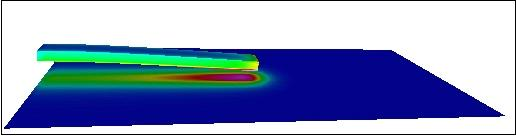
\includegraphics[width=0.8\textwidth]{electric_force}}
  \caption{An elastic beam bended by the electrostatic force due to a
          potential difference between the beam and the bottom
          plate. The electric potential is calculated in the volume
          surrounding the beam although the solution or the mesh are
          not shown.}
\end{figure}


%%%%%%%%%%%%%%%%%%%%%%%%%%%%%%%%%%%%%%%%%%%%%%%%%%%%%%%%%%%%
% Appendices 

\appendix

%\graphicspath{{./}{units/}}
%\include{units/units}

%%%%%%%%%%%%%%%%%%%%%%%%%%%%%%%%%%%%%%%%%%%%%%%%%%%%%%%%%%%%

% Include the index
\printindex

%%%%%%%%%%%%%%%%%%%%%%%%%%%%%%%%%%%%%%%%%%%%%%%%%%%%%%%%%%%%

\end{document}

%%%%%%%%%%%%%%%%%%%%%%%%%%%%%%%%%%%%%%%%%%%%%%%%%%%%%%%%%%%%


























% Heat and Mass Transfer
\graphicspath{{./}{heatequation/}}
\chapter{Heat Equation}

\modinfo{Module name}{included in solver}
\modinfo{Module subroutines}{\Idx{HeatSolve}}
\modinfo{Module authors}{Juha Ruokolainen}
\modinfo{Document authors}{Juha Ruokolainen, Ville Savolainen}
\modinfo{Document edited}{July 29th 2002}

\section{Introduction}

Heat equation results from the requirement of \Idx{energy conservation}.
In addition the Fourier's law is used to model
the heat conduction. The linearity of the equation may be 
ruined by temperature dependent thermal conductivity, or by
heat radiation.

\section{Theory}

\subsection{Governing Equations}
The incompressible heat equation is expressed as
\begin{equation}
\rho  c_p\left( \frac{\partial T}{\partial t}+(\vec u\cdot\nabla) T\right) - 
\nabla\cdot(k\nabla T) =
\overline{\overline\tau}:\overline{\overline \varepsilon} + \rho h,
\label{heat_equation}
\end{equation}
where $\rho$ is the density, $c_p$ the heat capacity at constant pressure, 
$T$ the temperature, $\vec u$ the convection velocity, $k$ the heat 
conductivity and $h$ is source of heat.
The term $\overline{\overline\tau}:\overline{\overline \varepsilon}$ is the
frictional viscous heating, which is negligible in most cases. For Newtonian
fluids, the viscous
part of the stress tensor is
\begin{equation}
\overline{\overline\tau} = 2\mu \overline{\overline\varepsilon},
\end{equation}
where $\overline{\overline \varepsilon}$ the linearized strain rate tensor.

Eq.\ref{heat_equation} applies also for solids, setting $\vec u = 0$. For
solids, conduction may be anisotropic and the conductivity a tensor.

For compressible fluids, the heat equation is written as
\begin{equation}
\rho c_v\left(\frac{\partial T}{\partial t} + \vec{u}\cdot\nabla T\right) -
\nabla\cdot\left(k\nabla T\right) = - p \nabla\cdot\vec{u} 
+ \overline{\overline\tau}:\overline{\overline \varepsilon}
+ \rho h,
\end{equation}
where $c_v$ is the heat capacity at constant volume. The density needs to be
calculated from the equation of state, e.g., perfect gas law. More
information is given in the chapter describing the Navier-Stokes equation.

The Elmer heat equation module is capable of simulation heat transfer by
conduction, convection, and diffuse gray radiation. Also a phase change
model is included. Couplings to other modules include, convection by
fluid flow, frictional heating (modules providing flow fields), and
resistive heating (modules providing magnetic and/or electric fields).


\subsection{Phase Change Model}

Elmer has an internal fixed grid phase change model. Modelling phase change is done
by modifying the definition of heat capacity according to whether
a point in space is in solid or liquid phase or in a 'mushy' region.
The choice of heat capacity within the intervals is explained in detail
below.

This type of algorithm is only applicable, when the phase change occurs
within finite temperature interval. If the modelled material is such that
the phase change occurs within very sharp temperature interval, this
method might not be appropriate.

For the solidification phase change model Elmer uses,  we need enthalpy.
The enthalpy is defined to be
\begin{equation}
H(T) = \int_0^T \left ( \rho c_p + \rho L\frac{\partial f}{\partial \lambda}\right )d\lambda,
\end{equation}
where $f(T)$ is the fraction of solid material as a function of
temperature, and $L$ is the latent heat.
The enthalpy-temperature curve is used
to compute an effective heat capacity, whereupon the equations become identical
to the heat equation. There are two ways of computing the effective heat capacity in Elmer:
\begin{equation}
c_{p,\mathrm{eff}} = \frac{\partial H}{\partial T},
\end{equation}
and
\begin{equation}
c_{p,\mathrm{eff}} = \left ( \frac{\nabla H\cdot\nabla H}{\nabla T\cdot\nabla T}\right )^{1/2}.
\end{equation}
The former method is used only if the local temperature gradient is very small, while
the latter is the preferred method. In transient simulations a third method is used, given
by
\begin{equation}
c_{p,\mathrm{eff}} = \frac{\partial H/\partial t}{\partial T/\partial t}.
\end{equation}

\subsection{Additional Heat Sources}

Frictional heating is calculated currently, for both incompressible and 
compressible fluids, by the heat source
\begin{equation}
h_f = 2\mu\overline{\overline\varepsilon}:\overline{\overline\varepsilon}.
\end{equation}

In case there are currents in the media the also the 
the resistive heating may need to be considered.
The \Idx{Joule heating} is then given by
\begin{equation}
h_m = \frac{1}{\sigma} \vec J \cdot \vec J.
\end{equation}
In the above equations, $\vec B$ and $\vec E$ are the magnetic and electric
fields, respectively. The current density $\vec J$ is defined as
\begin{equation}
\vec J = \sigma(\vec E + \vec u\times \vec B).
\end{equation}


\subsection{Boundary Conditions}
For temperature one can apply boundary conditions and have either temperature 
or heat flux prescribed.

\Idx{Dirichlet boundary condition} (temperature is 
prescribed) reads as
\begin{equation}
T=T_b.
\end{equation}
\noindent The value  of $T_b$ can be constant or a function of time, position or 
other variables. 

Heat flux depending on heat transfer coefficient $\alpha$ and external
temperature $T_{\mathrm{ext}}$ may be written as
\begin{equation}
-k\frac{\partial T}{\partial n} =\alpha (T-T_{ext} ).
\end{equation}
Both variables $\alpha$ and $T_\mathrm{ext}$ can be constant or functions of time, 
position or other variables. If the heat transfer coefficient $\alpha$ is equal
to zero, it means that the heat flux on a boundary is identically zero. The 
\Idx{Neumann boundary condition} $-k\partial T/\partial n =0$ is also used in a 
symmetry axis in 2D, axisymmetric or cylindrical problems.

Heat flux can consist of idealized radiation whereupon
\begin{equation}
-k\frac{\partial T}{\partial n} =\sigma\varepsilon (T^4 -T^4_\mathrm{ext} ).
\label{radcondition}
\end{equation}
Above,  $\sigma$ is the \Idx{Stefan-Boltzmann constant} and $\varepsilon$ the 
surface emissivity. The emissivity and the external temperature can 
again be constant or functions of time, position, or other variables.

If the surface $k$ is receiving radiation from other surfaces in the system,
then the heat flux reads as
\begin{equation}
-k_k \frac{\partial T_k}{\partial n_k} = \sigma \varepsilon_k (T_k^4 -
{1\over {A_k \varepsilon_k}} \sum_{i=1}^N G_{ik} \varepsilon_i  T_i^4 A_i ),
\end{equation}
where the subscripts $i$ and $k$ refer to surfaces $i$ and $k$, and the parameters $A_i$ and
$A_k$ to the specific surface areas. The factors $G_{ik}$ are \Idx{Gebhardt factors}, and
$N$ represents the total number of radiating surfaces present in the system.
Emissivities are assumed to be constant on each surface.

The heat equation is nonlinear when radiation is modelled.
The nonlinear term in the boundary condition (\ref{radcondition})
can be linearized as
\begin{eqnarray}
T^4 - T^4_\mathrm{ext} \approx
( {\cal T}^3 + T_\mathrm{ext} {\cal T}^2  + T^2_\mathrm{ext} {\cal T} + 
T^3_\mathrm{ext} )( T-T_\mathrm{ext} ),
\end{eqnarray}
where $\cal{T}$ is the temperature from the previous iteration.

One may also give an additional heat flux term as
\begin{equation}
-k\frac{\partial T}{\partial n} = q.
\end{equation}

\section{Keywords} 

\sifbegin
\sifitemnt{Constants}{}
\sifbegin
\sifitem{Stefan Boltzmann}{Real}
The value of the Stefan-Boltzmann constant needed for 
thermal radiation.
\sifend

\sifitem{Simulation}{}
The simulation section gives the case control data:
\sifbegin
\sifitem{Simulation Type}{String} Heat equation may be either 
{\tt Transient} or {\tt Steady State}.
\sifitem{Coordinate System}{String} Defines the coordinate system to be used, one of:
{\tt Cartesian 1D}, {\tt Cartesian 2D},~ ~{\tt Cartesian 3D},~ ~{\tt Polar 2D},~ 
~{\tt Polar 3D},~ ~{\tt Cy\-lin\-dric},~ ~{\tt Cylindric Symmetric}~
~and~ ~{\tt Axi Symmetric}.
\sifitem {Gebhardt Factors}{File}
If the model includes diffuse gray radiation, the file containing the Gebhardt factors
must be given. This file is written by the program {\tt GebhardtFactors} as a preprocessing step.
\sifitem{View Factors}{File} 
If the model includes diffuse gray radiation, the file containing the view factors
must be given to the program computing the Gebhardt factors. 
This file is written by the program {\tt ViewFactors} as a
preprocessing step. The tasks of computing view factors and the Gebhardt 
factors have been divided, because
the view factors depend only on geometry (and thus the mesh), while the Gebhardt factors also depend on
the boundary emissivities. 
\sifitem{Timestepping Method}{String} 
Possible values of this parameter are {\tt Newmark} (an additional
parameter {\tt Newmark Beta} must be given), {\tt BDF} ({\tt BDF Order} must be given). Also as a
shortcut to {\tt Newmark}-method with values of {\tt Beta}$=0.0, 0.5,$ $1.0$ the keywords 
{\tt Explicit Euler}, {\tt Crank-Nicolson}, and {\tt Implicit Euler} may be given respectively.
The recommended choice for the first order time integration is the BDF method of order 2.
\sifitem{BDF Order}{Integer}
Value may range from 1 to 5.
\sifitem{Newmark Beta}{Real} Value in range from 0.0 to 1.0. The value 0.0 equals to
the explicit Euler integration method and the value 1.0 equals to the implicit Euler method. 
\sifend

\sifitem{Solver}{solver id}
The solver section defines equation solver control variables. Most of the possible
keywords -- related to linear algebra, for example -- are common for all the solvers and are 
explained elsewhere.
\sifbegin
\sifitem{Equation}{String Heat Equation}
The name of the equation.
\sifitem{Nonlinear System Convergence Tolerance}{Real}
The criterion to
terminate the nonlinear iteration after the relative change of the norm of the field variable
between two consecutive iterations is small enough
$$
 ||T_i-T_{i-1}|| < \epsilon ||T_i||,
$$
where $\epsilon$ is the value given with this keyword.
\sifitem{Nonlinear System Max Iterations}{Integer}
The maximum number of nonlinear iterations the
solver is allowed to do.
\sifitem{Nonlinear System Newton After Iterations}{Integer}
Change the nonlinear solver type to
Newton iteration after a number of Picard iterations have been performed. If a given
convergence tolerance between two iterations is met before the iteration count is met,
it will switch the iteration type instead. In the heat equation the Picard iterations 
means that the radiation term is factorized to linear and third-power terms.
\sifitem{Nonlinear System Newton After Tolerance}{Real}
Change the nonlinear solver type to
Newton iteration, if the relative change of the norm of the field variable meets a
tolerance criterion:
$$
 ||T_i-T_{i-1}|| < \epsilon ||T_i||,
$$
where $\epsilon$ is the value given with this keyword.
\sifitem{Nonlinear System Relaxation Factor}{Real}
Giving this keyword triggers the use
of  relaxation in the nonlinear equation solver.
Using a factor below unity is sometimes required to achieve convergence of the nonlinear system.
A factor above unity might speed up the convergence. Relaxed variable is defined as follows:
$$
 T^{'}_i = \lambda T_i + (1-\lambda) T_{i-1},
$$
where $\lambda$ is the factor given with this keyword. The default value for the relaxation factor
is unity.
\sifitem{Steady State Convergence Tolerance}{Real}
With this keyword a equation specific steady state or coupled system
convergence tolerance is given.
All the active equation solvers must meet their own tolerances before the 
whole system is deemed converged.
The tolerance criterion is:
$$
 ||T_i-T_{i-1}|| < \epsilon ||T_i||,
$$
where $\epsilon$ is the value given with this keyword.
\sifitem{Stabilize}{Logical} 
If this flag is set true the solver will use stabilized finite element method
when solving the heat equation with a convection term. If this flag is set to
{\tt False} RFB (Residual Free Bubble) stabilization is used instead (unless
the next flag {\tt Bubbles} is set to {\tt False} in a problem with Cartesian
coordinate system).
If convection dominates stabilization must be used in order to successfully solve the equation.
The default value is {\tt False}.
\sifitem{Bubbles}{Logical}
There is also a residual-free-bubbles formulation of the stabilized finite-element
method. It is more accurate and does not include any ad hoc terms. However, it may
be computationally more expensive. The default value is {\tt True}.
If both {\tt Stabilize} and {\tt Bubbles} or set to {\tt False}, no stabilization
is used. Note that in this case, the results might easily be nonsensical.
\sifitem{Smart Heater Control After Tolerance}{Real}
The smart heater control should not be activated before the 
solution has somewhat settled. By default the smart heater 
control is set on when the Newtonian linearization is 
switched on for the temperature equation. Sometimes
it may be useful to have more stringent condition for 
turning on the smart heater control and then this keyword
may be used to give the tolerance. 
%
\sifend
In some cases the geometry or the emissivities of the radiation boundaries 
change. This may require the recomputation of the \Idx{view factors} and 
\Idx{Gebhardt factors}. For that purpose also dynamic computation of the factors
is enabled and it is controlled by the keywords below.
The radiation factors are also automatically computed if
no files for the factors are given allthough radiation boundaries
exist. 
\sifbegin
\sifitem{Update View Factors}{Logical}
The recomputation of the view factors is activated by 
setting the value of this flag to \texttt{True}.
\texttt{False} is the default.
\sifitem{Update Gebhardt Factors}{Logical}
If the emissivities depend on the solution the Gebhardt factors may need to 
be recomputed. This is activated by setting giving this flag value \texttt{True}.
\texttt{False} is the default.
\sifitem{Minimum View Factor}{Real}
This keyword determines the cut-off value under which the view factors are
omitted. Neglecting small values will not only save memory but also will
make the matrix used for solving the Gabhardt factors less dense. 
This consequently will enable more efficient sparse matrix strategies
in solving the Gebhardt factors.
The value for this parameter might be of the order 10e-8. 
\sifitem{Minimum Gebhardt Factor}{Real}
The Gebhardt factors make part of matrix dense. By neglecting the smallest Gebhardt factors
the matrix structure for the heat equation 
may become significantly sparser and thus the solution time may drop.
The value for this parameter might also be of the order 10e-8. 
%
\sifitem{Implicit Gebhardt Factor Fraction}{Real}
In computing heat transfer problems with radiation in an implicit manner the matrix structure 
becomes partially filled. This affects the performance of the linear equation solvers
and also increases the memory requirements. On the other hand explicit treatment 
of radiation slows down the convergence significantly. This keyword allows
that the largest Gebhardt factors are treated in an implicit manner whereas
the smallest are treated explicitely. The value should lie in between 
zero (fully explicit) and one (fully implicit).
%
\sifitem{Matrix Topology Fixed}{Logical}
If the Gebhardt factors change the matrix structure of the heat equation
may also have to be changed unless this flag is set to \texttt{False}.
Then all factors that do not combine with the matrix structure are omitted.
\sifitem{View Factors Geometry Tolerance}{Real}
The view factors take a lot of time to compute. Therefore during the iteration a test is performed 
to check whether the geometry has changed. If the relative maximum change in the coordinate 
values is less than the value given by this parameter the view factors are not recomputed and
the old values are used. 
\sifitem{View Factors Fixed After Iterations}{Integer} 
Sometimes the iteration changes the geometry of the radiation
boundaries as an unwanted side-effect. Then the geometry on the radiation 
boundary may be set fixed after some iterations. In practice this is done by adding
suitable Dirichlet conditions in the boundary conditions.
\sifitem{Gebhardt Factors Solver Full}{Logical}
If the view factor matrix is relatively sparse it will make sense
to use a sparse matrix equation for solving the Gebhardt factors.
This flag may be used if a full matrix should be desired.
\sifitem{Gebhardt Factors Solver Iterative}{Logical}
If the Gebhardt factors are solved from a sparse matrix equation 
also the type of solver may be selected. The default is 
direct \texttt{umfpack} solver. Sometimes the memory usage may be a problem
or the direct strategy simply not efficient enough. Then 
an iterative \texttt{cgs} solver may be used instead.
\sifend

\sifitem{Equation}{eq id}
The equation section is used to define a set of equations for a body or set of bodies.
\sifbegin
\sifitem{Heat Equation}{String} If set to {\tt True}, solve the heat equation.
\sifitem{Convection}{String}
The type of convection to be used
in the heat equation, one of: {\tt None}, {\tt Computed}, {\tt Constant}.
\sifitem{Phase Change Model}{String}
One of: {\tt None},~ {\tt Spatial 1},
~{\tt Spatial 2}~ and~ {\tt Temporal}.
Note that when solidification is modelled, the
enthalpy-temperature- and viscosity-temperature-curves must be defined in 
the material section.
\sifend


\sifitem{Body Forces}{bf id} 
The body force section may be used to give additional force terms for the equations.
The following keywords are recognized by the base solver:
\sifbegin
\sifitem{Heat Source}{Real}
An additional heat source $h$ for the heat equation may be given
with this keyword.
\sifitem{Friction Heat}{Logical}
Currently redundant key word, the frictional heating $h_f$ is automatically
added.
\sifitem{Joule Heat}{Logical}
If set {\tt True}, triggers use of the inductive heating.
\sifitem{Smart Heater Control}{Logical}
Sometimes the predescribed heat source does not lead to the desired 
temperature. Often the temperature is controlled by a feedback and therefore
a similar heater control in the simulation may give more realistic results.
This flag makes sets the smart heater control on for the given body force.
\sifend


\sifitem{Initial Condition}{ic id}
The initial condition section may be used to set initial values for temperature.
\sifbegin
\sifitemnt{Temperature}{Real}
\sifend

\sifitem{Material}{mat id}
The material section is used to give the material parameter values. The
following material parameters may be effective when heat equation is solved.
\sifbegin
\sifitem{Density}{Real}
The value of density is given with this keyword. The value may be constant,
or variable. For the compressible flow, the density is computed internally,
and this keyword has no effect.
\sifitem{Enthalpy}{Real} 
Note that, when using the solidification modelling,
an enthalpy-temperature curve must be given. The enthalpy is derived with
respect to temperature to get the value of the effective heat capacity.
\sifitem{Viscosity}{Real} Viscosity is needed if viscous heating 
is taken into account. When using the solidification modelling,
a viscosity-temperature curve must be given. The viscosity must be set
to high enough value in the temperature range for solid material to effectively
set the velocity to zero.
\sifitem{Heat Capacity}{Real}
The value of heat capacity in constant pressure $c_p$ is given
with this keyword. The value may be constant,
or variable. For the phase change model, this value is modified according to
rules given in the theory section.
\sifitem{Heat Conductivity}{Real}
The value of heat conductivity $k$ is given with this keyword. The value may
be a constant or variable.
\sifitem{Convection Velocity i}{Real} 
Convection velocity {\tt i}$=1,2,3$ for the constant convection model.
\sifitem{Compressiblity Model}{Real} This setting may be used to set the compressibilty
model for the flow simulations. Choices are {\tt Incompressible} and {\tt Perfect Gas}.
If set to the latter there may
be mechanical work performed by the heating.
Then also the settings {\tt Reference Pressure} and {\tt Specific Heat Ratio} must also be given.
\sifitem{Reference Pressure}{Real} With this keyword a reference level of pressure may be given.
\sifitem{Specific Heat Ratio}{Real} The ratio of specific heats (in constant pressure
versus in constant volume) may be given with this keyword.
The default value of this setting is $5/3$, which
is the appropriate value for monoatomic ideal gas.
\sifend

\sifitem{Boundary Condition}{bc id}
The boundary condition section holds the parameter values for various
boundary condition types. In heat equation we may set the temperature directly 
by Dirichlet boundary conditions or use different flux conditions for the temperature.
The natural boundary condition of heat equation is zero flux condition.
\sifbegin
\sifitemnt{Temperature}{Real}
\sifitem{Heat Flux BC}{Logical} 
Must be set to {\tt True},  if heat flux boundary
condition is present.
\sifitem{Heat Flux}{Real} A user defined heat flux term.
\sifitem{Heat Transfer Coefficient}{Real}
Defines the parameter $\alpha$ in the heat flux boundary
condition of the type
$$
    -k\frac{\partial T}{\partial n} = \alpha(T-T_{ext}) .
$$
\sifitem{External Temperature}{Real} 
Defines the variable for ambient temperature $T_{ext}$ in the previous equation.
\sifitem{Radiation}{String}
The type of radiation model for this boundary,
one of: {\tt None}, {\tt Idealized}, {\tt Diffuse Gray}. 
Note that, when using the diffuse gray radiation model, the file containing
the Gebhardt factors must be given in the simulation section.
\sifitem{Radiation Boundary}{Integer}
If there are many closures with radiation boundary conditions that do not
see each other the view factors may be computed separately. This keyword
is used to group the boundaries to independent sets. The default is one.
\sifitem{Radiation Boundary Open}{Logical}
The closures may be partially open. Then no normalization of the view factors
is enforced. The missing part of the radiation angle is assumed to be 
ideal radiation. Therefore if this option is enforced also 
the parameter \texttt{External Temperature} must be given. 
\sifitem{Emissivity}{Real}
Emissivity of the radiating surface, required for radiation model is present.
\sifitem{Radiation Target Body}{Integer} 
This flag may be used to set the
direction of the outward pointing normal. This is used when computing viewfactors.
A body identification number must be given.  The default is that the normal points to less
dense material or outward on outer boundaries.
%
\item{Smart Heater Boundary}{Logical}
If the smart heater is activated the point for monitoring the temperature is 
the point with maximum $x$-coordinate on the boundary where this 
keyword is set \texttt{True}. Alternatively the logical variable \texttt{Phase Change}
is looked for. 
\item{Smart Heater Temperature}{Real}
The desired temperature for the smart heater system is set by this keyword. 
Alternatively the real variable \texttt{Melting Point} may be used. 
\sifend
\sifend




\graphicspath{{./}{navier-stokes/}}
\chapter{Navier-Stokes Equation}

\modinfo{Module name}{included in solver}
\modinfo{Module subroutines}{\Idx{FlowSolve}}
\begin{versiona}
\modinfo{Module authors}{Juha Ruokolainen}
\modinfo{Document authors}{Juha Ruokolainen, Peter R�back}
\modinfo{Document edited}{10.8.2004}

\section{Introduction}
In solid and liquid materials heat transfer and viscous fluid flow are 
governed by heat and \Idx{Navier-Stokes equation}s, which can be derived from the 
basic principles of conservation of mass, momentum and energy. Fluid can be
either \Idx{Newtonian} or \Idx{non-Newtonian}. In the latter case the consideration in
Elmer is limited to purely viscous behaviour with the power-law model.

In the following we present the governing equations of fluid flow, heat
transfer and stresses in elastic material applied in  Elmer. Also the most
usual boundary conditions applied in computations are described.

\section{Theory}

%\subsection{The Governing Equations}

The momentum and continuity equations can be written as
\begin{eqnarray}
\rho \left( 
\frac{\partial\vec u}{\partial t} + (\vec u \cdot \nabla)\vec u
\right) - \nabla\cdot \overline{\overline \sigma} = \rho\vec f,
\label{momentum}
\end{eqnarray}
and
\begin{eqnarray}
\left( \frac{\partial\rho}{\partial t} + (\vec u\cdot \nabla)\rho
\right)  + \rho(\nabla\cdot\vec u) = 0,
\label{continuity}
\end{eqnarray}
where $\overline{\overline \sigma}$ is the stress tensor. For Newtonian
fluids
\begin{eqnarray}
\overline{\overline\sigma} = 2\mu \overline{\overline\varepsilon}
-\frac{2}{3} \mu (\nabla\cdot\vec u)\overline{\overline I} - p 
\overline{\overline I},
\label{newtonian}
\end{eqnarray}
where $\mu$ is the viscosity, $p$ is the pressure, $\overline{\overline I}$
the unit tensor and $\overline{\overline \varepsilon}$ the linearized strain
rate tensor, i.e.
\begin{eqnarray}
\varepsilon_{ij} = \frac{1}{2}\left( \frac{\partial u_i}{\partial x_j} +
\frac{\partial u_j}{\partial x_i}
\right). \label{linstrain}
\end{eqnarray}
The density of an ideal gas depends on the pressure and temperature through
the equation of state
\begin{eqnarray}
\rho = \frac{p}{RT}\label{stateequation},
\end{eqnarray}
where $R$ is the gas constant:
\begin{eqnarray}
R = \frac{\gamma - 1}{\gamma}c_p.
\end{eqnarray}
The specific heat ratio $\gamma$ is defined as
\begin{eqnarray}
\gamma = \frac{c_p}{c_v},\label{specificheatratio}
\end{eqnarray}
where $c_p$ and $c_v$ are the heat capacities in constant pressure
and volume, respectively. The value of $\gamma$ depends solely on
the internal molecular properties of the gas.

An imcompressibe flow is characterized by the condition
$\rho$=constant, from which it follows that
\begin{eqnarray}
\nabla\cdot \vec u = 0. \label{incompressible}
\end{eqnarray}
Enforcing the constraint (\ref{incompressible}) in (\ref{momentum}),
(\ref{continuity}) and (\ref{newtonian}), the equations reduce to
the Navier-Stokes equations
\begin{eqnarray}
\rho \left( \frac{\partial\vec u}{\partial t}
+ (\vec u \cdot\nabla) \vec u \right)
 -\nabla\cdot(2\mu \overline{\overline\varepsilon})+
\nabla p & = &\rho\vec f, \label{NS-equation} \\
\nabla\cdot\vec u &=& 0.
\label{Navier-Stokes_equations}
\end{eqnarray}
Compressible flows are modelled by the equations
(\ref{momentum})-(\ref{specificheatratio}). Then,
it is possible to replace the state equation
(\ref{stateequation}) by
\begin{equation}
\rho = \frac{1}{c^2}p, \label{statespeed}
\end{equation}
where $c=c(p,T,\dots)$ is the speed of sound. The equation
(\ref{statespeed}) can be used with liquid materials as well.

Most commonly the term $\rho\vec f$ represents a force due to gravity, 
in which case the vector $\vec f$ is the gravitational acceleration.
It can also represent, for instance, the \Idx{Lorentz force} when magnetohydrodynamic 
effects are present. 

For isothermal flows the equations
(\ref{NS-equation}) and (\ref{Navier-Stokes_equations}) desrcibe the system
in full. For thermal flows also the heat equation needs to be solved.

For thermal incompressible fluid flows we  assume that the Boussinesq approximation is 
valid. This means that the density of the fluid is constant except in the body
force term where the density depends linearly on temperature through the 
equation
\begin{equation}
\rho = \rho_0 (1-\beta (T-T_0 )),
\end{equation}
where $\beta$ is the volume expansion coefficient and the subscript 0 refers 
to a reference state. Assuming that the gravitational acceleration $\vec g$
is the only external force, then the force $\rho_0 \vec g (1-\beta (T-T_0 ))$
is caused in the fluid by temperature variations. This phenomenon is called
\Idx{Grashof convection} or \Idx{natural convection}.


One can choose between transient and steady state analysis.
In transient analysis one has to set, besides boundary conditions, also 
initial values for the unknown variables. 

\subsection{Boundary Conditions}

For the Navier-Stokes equation one can apply boundary conditions 
for velocity components or the tangential or
normal stresses may be defined.

In 2D or axisymmetric cases the \Idx{Dirichlet boundary condition} for velocity 
component $u_i$ is simply
\begin{equation}
u_i = u_i^b. 
\end{equation}
A value $u_i^b$ can be constant or a function of time, position or other 
variables. In cylindrical cases the Dirichlet boundary condition for angular 
velocity $u^\theta$ is
\begin{equation}
u^\theta =\omega,
\end{equation}
where $\omega$ is the rotation rate.

In axisymmetric geometries one has to set $u_r =0$ and 
$\partial u_z/\partial r =0$  on the symmetry axis.

If there is no flow across the surface, then
\begin{equation}
\vec u\cdot\vec n =0
\end{equation}
where $\vec n$ is the outward unit normal to the boundary.

Surface stresses can be divided into normal and tangential stresses. Normal 
stress is usually written in the form
\begin{equation}
\sigma_n ={{\gamma}\over R} -p_a 
\label{normal_stress}
\end{equation}
where $\gamma$ is the surface tension coefficient, $R$ the mean curvature and 
$p_a$ the atmospheric (or external) pressure. Tangential stress has the form
\begin{equation}
\vec\sigma_\tau = \nabla_s \gamma,
\label{tangential_stress}
\end{equation}
where $\nabla_s$ is the surface gradient operator.

The coefficient $\gamma$ is a thermophysical property depending on the
temperature. Temperature differences on the surface influence the 
transport of momentum and heat near the surface. This phenomenon is called 
Marangoni convection or thermocapillary convection. The temperature
dependence of the surface tension coefficient can be approximated by a linear
relation:
\begin{equation}
\gamma =\gamma_0 (1-\vartheta (T-T_0 )),
\label{surface_tension_coefficient}
\end{equation}
where $\vartheta$ is the temperature coefficient of the surface tension and
the subscript $0$ refers to a reference state. If a Boussinesq
\index{Boussinesq approximation}
hypothesis is made, i.e., the surface tension coefficient is constant except in
(\ref{tangential_stress}) due to (\ref{surface_tension_coefficient}), the boundary
condition for tangential stress becomes
\begin{equation}
\vec\sigma_\tau =-\vartheta\gamma_0\nabla_s \gamma.
\end{equation}
In equation (\ref{normal_stress}) it holds then that $\gamma =\gamma_0$.
The linear temperature dependence of the surface tension coefficient is 
naturally only one way to present the dependence. In fact, the 
coefficient $\gamma$ can be any user defined function in Elmer.
One may also give the force vector on a boundary directly as in
\begin{equation}
\overline{\overline\sigma}\cdot \vec n = \vec g.
\label{boundary_stress}
\end{equation}

\subsection{Linearization}

As is well known, the convective transport term of the Navier-Stokes equations
and the heat equation is a source of both physical and numerical instability.
The numerical instability must be compensated somehow in order
to solve the equations on a computer. For this reason the so called stabilized
finite element method (\cite{franca92},\cite{franca92b}) is used in Elmer to discretize
these equations.  
%The equations in the form implemented in Elmer and
%the discretization are described in more detail in Appendix
%\ref{chapter-solver-discretation}. 
%In Appendix \ref{chapter-free-surfaces} the free surface problem is presented.

The convection term of the Navier-Stokes equations is nonlinear and has to be
linearized for computer solution. There are two linearizations 
of the convection term in Elmer:
\begin{equation}
(\vec u\cdot\nabla)\vec u \approx
(\vec {\cal U}\cdot\nabla)\vec {\cal U}
\end{equation}
and
\begin{equation}
(\vec u\cdot\nabla)\vec u \approx
(\vec u\cdot\nabla)\vec{\cal U} +
(\vec{\cal U}\cdot\nabla)\vec u -
(\vec {\cal U}\cdot\nabla)\vec {\cal U},
\end{equation}
where $\vec{\cal U}$ is the velocity vector from the previous iteration.
The first of the methods is called \Idx{Picard iteration} 
or the method of the fixed point, while the latter
is called \Idx{Newton iteration}. The convergence rate of the Picard iteration is of first order, and the
convergence might at times be very slow. The convergence rate of the Newton method is of second order,
but to succesfully use this method, a good initial
guess for velocity and pressure fields is required. The solution to this problem is to
first take a couple of Picard iterations, and switch to Newton iteration after
the convergence has begun.


\subsection{Non-newtonian Material Models}

There are several non-newtonian material models. All are functions 
of the strainrate $\dot{\gamma}$. The simple power law model has a problematic 
behavior at low shear rates. The more complicated models provide a 
smooth transition from low to high shearrates.

{\bf Power law}
\begin{equation}
  \eta = \begin{cases} 
\eta_0 \dot{\gamma}^{n-1} 		& \text{if $\dot{\gamma} > \dot{\gamma}_0$}, \\
         \eta_0  \dot{\gamma}_0^{n-1}   & \text{if $\dot{\gamma} \le \dot{\gamma}_0$}.
  \end{cases}
\end{equation}
where $\eta_\infty$ is constant, $\dot{\gamma}_0$ is the critical shear rate,
and $n$ is the viscosity exponent. 

{\bf Carreau-Yasuda}
\begin{equation}
  \eta = \eta_\infty + \Delta \eta \left ( 1+(c\dot{\gamma})^y \right )^{\frac{n-1}{y}},
\end{equation}
where $\eta_\infty$ is the high shearrate viscosity $\dot{\gamma}\rightarrow\infty$
provided that $n<1$. For shearrates approaching zero the viscosity is 
$\eta_0=\eta_\infty+\Delta \eta$. $\Delta \eta$ is thus the maximum
viscosity difference between low and high shearrate.
This model recovers the plain Carreau model when the Yasuda exponent $y=2$.

The model can be made temperature dependent. One choice is to multiply $\Delta \eta$ and $c$
by factor $\exp(d(1/T-1/T_0))$, where $d$ and $T_0$ are model parameters.

{\bf Cross}
\begin{equation}
  \eta = \eta_\infty + \frac{\Delta \eta}{1+c\dot{\gamma}^n},
\end{equation}
where again $\eta_\infty$ is the high shearrate viscosity.

{\bf Powell-Eyring}
\begin{equation}
  \eta = \eta_\infty + \Delta \eta \frac{\text{asinh} (c \dot{\gamma} )}{c\dot{\gamma}}.
\end{equation}


\subsection{Flow in Porous Media}

A simple \Idx{porous media} model is provided in the Navier-Stokes solver.
It utilizes the \Idx{Darcy's law} that states that the flow resistance is
proportinal to the velocity and thus the modified momentum equation reads
\begin{eqnarray}
\rho \left( 
\frac{\partial\vec u}{\partial t} + (\vec u \cdot \nabla)\vec u
\right) - \nabla\cdot \overline{\overline \sigma} + r \vec{u}= \rho\vec f,
\label{momentum}
\end{eqnarray}
where $r$ is the porous resistivity which may also be an orthotropic tensor.
Usually the given parameter is permeability which
is the inverse of the resistivity as defined here.
No other features of the porous media flow is taken into consideration.
Note that for large value of $r$ only the bubble stabilization 
is found to work. 

\subsection{Coupling to Electric Fields}

In \Idx{electrokinetics} the fluid may have charges that are coupled
to external electric fields. This results to an external force that is 
of the form 
\begin{equation}
  \vec{f}_e = -\rho_e \nabla \phi ,
\end{equation}
where $\rho_e$ is the charge density and $\phi$ is the external electric field.
The charge density may also be a variable. More specifically this force may be 
used to couple the Navier-Stokes equation to the \Idx{Poisson-Boltzmann equation} 
describing the charge distribution in electric doubly layers. Also
other types of forces that are proportional to the gradient of the field
may be considered.


\subsection{Coupling to Magnetic Fields}

If the fluid has free charges it may couple with an magnetic field.
The magnetic field induced force term for the
flow momentum equations is defined as
\begin{equation}
\vec{f}_m = \vec{J}\times\vec{B},
\end{equation}
Here $\vec B$ and $\vec E$ are the magnetic and electric
fields, respectively. The current density $\vec J$ is defined as
\begin{equation}
\vec J = \sigma(\vec E + \vec u\times \vec B).
\end{equation}



\section{Keywords} 
\end{versiona}


\sifbegin
\sifitemnt{Constants}{}
\sifbegin
\sifitem{Gravity}{Size 4 Real [x y z abs]}
The above statement gives a real vector whose length is four. In this case the
first three components give the direction vector of the gravity and the fourth
component gives its intensity.
\sifend

\sifitem{Solver}{solver id} 
Note that all the keywords related to linear solver (starting with {\tt Linear System}) may be used in this solver as well.
They are defined elsewhere. 

\sifbegin
\sifitem{Equation}{String [Navier-Stokes]} 
The name of the equation.
\sifitem{Nonlinear System Convergence Tolerance}{Real} this keyword gives a criterion to
terminate the nonlinear iteration after the relative change of the norm of the field variable
between two consecutive iterations is small enough
$$
 ||u_i-u_{i-1}|| < \epsilon ||u_i||,
$$
where $\epsilon$ is the value given with this keyword.
\sifitem{Nonlinear System Max Iterations}{Integer} 
The maxmimum number of nonlinear iterations the
solver is allowed to do.
\sifitem{Nonlinear System Newton After Iterations}{Integer} 
Change the nonlinear solver type to
Newton iteration after a number of Picard iterations have been performed. If a given
convergence tolerance between two iterations is met before the iteration count is met,
it will switch the iteration type instead.
\sifitem{Nonlinear System Newton After Tolerance}{Real} 
Change the nonlinear solver type to
Newton iteration, if the relative change of the norm of the field variable meets a
tolerance criterion:
$$
 ||u_i-u_{i-1}|| < \epsilon ||u_i||,
$$
where $\epsilon$ is the value given with this keyword.
\sifitem{Nonlinear System Relaxation Factor}{Real} Giving this keyword triggers the use
of  relaxation in the nonlinear equation solver.
Using a factor below unity is sometimes required to achive convergence of the nonlinear system.
A factor above unity might speed up the convergence. Relaxed variable is defined as follows:
$$
 u^{'}_i = \lambda u_i + (1-\lambda) u_{i-1},
$$
where $\lambda$ is the factor given with this keyword. The default value for the relaxation factor
is unity.
\sifitem{Steady State Convergence Tolerance}{Real}
With this keyword a equation specific steady state or coupled system
convergence tolerance is given.
All the active equation solvers must meet their own tolerances before the 
whole system is deemed converged.
The tolerance criterion is:
$$
 ||u_i-u_{i-1}|| < \epsilon ||u_i||,
$$
where $\epsilon$ is the value given with this keyword.
\sifitem{Stabilize}{Logical} 
If this flag is set true the solver will use stabilized finite element method
when solving the Navier-Stokes equations.
Usually stabilization of the equations must be done in order to succesfully solve the equations.
If solving for the compressible Navier-Stokes equations, a bubble function formulation
is used instead of the stabilized formulation regardless of the setting of this keyword.
Also for the incompressible Navier-Stokes equations, the bubbles may be selected
by setting this flag to {\tt False}.
\sifend

\sifitem{Equation}{eq id}
The equation section is used to define a set of equations for a body or set of bodies:
\sifbegin
\sifitem{Navier-Stokes}{Logical} if set to {\tt True}, solve the Navier-Stokes equations.
\sifitem{Magnetic Induction}{Logical} If set to {\tt True}, solve the magnetic induction equation
along with the Navier-Stokes equations.
\sifitem{Convection}{String [None, Computed, Constant]}
The convection type to be used
in the heat equation, one of: {\tt None}, {\tt Computed}, {\tt Constant}. 
The second choice is used for thermal flows.
\sifend

\sifitem{Body Force}{bf id}
The body force section may be used to give additional force terms for the equations.
\sifbegin
\sifitem{Boussinesq}{Logical} If set true, sets the Boussinesq model on.
\sifitem{Flow BodyForce i}{Real} May be used to give additional body force for
the flow momentum equations, \texttt{i=1,2,3}.
\sifitem{Lorentz Force}{Logical} If set true, triggers the magnetic
field force for the flow mementum equations.

\sifitem{Potential Force}{Logical} If this is set true the force 
used for the electricstatic coupling is activated.  
%
\sifitem{Potential Field}{Real}
 The field to which gradient the external force is proportional to. For example
the electrostatic field.

\sifitem{Potentai Coefficient}{Real} 
The coefficient that multiplies the gradient term. For example, the 
charge density.


\sifend

\sifitem{Initial Condition}{ic id} 
The initial codition section may be used to set initial values for the field
variables. The following variables are active:
\sifbegin
\sifitemnt{Pressure}{Real}
\sifitem{Velocity i}{Real} 
For each velocity component {\tt i}$=1,2,3$.
\sifitem{Kinetic Energy}{Real}
For the k-$\varepsilon$ turbulence model.
\sifitem{Kinetic Energy Dissipation}{Real}
\sifend

\sifitem{Material}{mat id}
The material section is used to give the material parameter values. The
following material parameters may be set in Navier-Stokes equation.
\sifbegin
\sifitemnt{Density}{Real}
The value of density is given with this keyword. The value may be constant,
or variable. For the of compressible flow, the density is computed internally,
and this keyword has no effect.
\sifitem{Viscosity}{Real} 
The relationship between stress and strain velocity. 
When using the solidification modelling,
a viscosity-temperature curve must be given. The viscosity must be set
to high enough value in the temperature range for solid material to effectively
set the velocity to zero. 
\sifitem{Reference Temperature}{Real} This is the reference temperature for the Boussinesq model
of temperature dependence of density.
\sifitem{Heat Expansion Coefficient}{real} For the Boussinesq model the heat expansion
coefficient must be given with this keyword. Default is 0.0.
\sifitem{Applied Magnetic Field 1,2,3}{Real} An applied magnetic field may be given with these
keywords.
\sifitem{Compressiblity Model}{String}
This setting may be used to set the compressibilty
model for the flow simulations. Currently the setting may be set to either
{\tt Incompressible}, {\tt Perfect Gas} and 
{\tt ArtificialCompressible}. If perfect gas model is chosen 
the settings {\tt Reference Pressure} and {\tt Specific Heat Ratio} must also be given.
The artificial compressibility model may be used to boost convergence in
fluid-structure-interaction cases.
The default value of this setting is {\tt Incompressible}.
\sifitem{Reference Pressure}{Real} with this keyword a reference level of pressure may be given.
This setting applies only if the {\tt Compressiblity Model} is set to
the value {\tt Perfect Gas}.
\sifitem{Specific Heat Ratio}{Real} 
The ratio of specfic heats (in constant pressure
versus in constant volume) may be given with this keyword.
This setting applies only if the {\tt Compressiblity Model} is set to
value {\tt Perfect Gas}. The default value of this setting is $5/3$, which
is the appropriate value for monoatomic ideal gas.
\sifend

For the k-$\varepsilon$ turbulence model the model parameters may
also be given in the material section using the following
keywords
\sifbegin
\sifitemnt{KE SigmaK}{Real [1.0]}
\sifitemnt{KE SigmaE}{Real [1.3]}
\sifitemnt{KE C1}{Real [1.44]}
\sifitemnt{KE C2}{Real [1.92]}
\sifitemnt{KE Cmu}{Real [0.09]}
\sifend

Non-newtonian material laws are also defined in material section.
For the power law the constant coefficient is given by the keyword
\texttt{Viscosity}. 
\sifbegin
  \sifitem{Viscosity Model}{String}
The choices are \texttt{power law, carreau, cross, powell ey\-ring} and
\texttt{thermal carreau}.
If none is given the fluid is treated as newtonian.
  \sifitem{Viscosity Exponent}{Real}
	Parameter $n$ in the models power law, Carreau, Cross
  \sifitem{Viscosity Difference}{Real}
  Difference $\Delta \eta$ between high and low shearrate viscosities.
   Ablicable to Carreau, Cross and Powell-Eyring models.
\sifitem{Viscosity Transition}{Real}
   Parameter $c$ in the Carreau, Cross and Powell-Eyring models.
\sifitem{Critical Shear Rate}{Real [0.0]}
Optional parameter $\dot{\gamma}_0$ in power law viscosity model.
\sifitem{Yasuda Exponent}{Real}
Optional parameter $y$ in Carreau model. The default is 2. 
If activated the model is the more generic
Yasuda-Carreau model.
\sifitem{Viscosity Temp Ref}{Real}
Paremeter $T_0$ in the thermal Carreau-Yasuda model. 
\sifitem{Viscosity Temp Exp}{Real}
Paremeter $d$ in the thermal Carreau-Yasuda model. 
\sifend
% 
Porosity is defined by the material properties
\sifbegin
  \sifitem{Porous Media}{Logical}
If this keyword is set \texttt{True} then the porous model will
be active in the material.
  \sifitem{Porous Resistance}{Real}
This keyword may give a constant resistance or also
a orthotropic resistance where the resistance of each velocity component is
given separately.
 \sifend

\sifitem{Boundary Condition}{bc id}
The boundary condition section holds the parameter values for various
boundary condition types. Dirichlet boundary conditions may be
set for all the primary field variables. The one related to Navier-Stokes equation
are
\sifbegin
\sifitem{Velocity i}{Real} 
Dirichlet boundary condition
for each velocity component {\tt i}$=1,2,3$.
\sifitem{Pressure}{Real} 
Absolute pressure.
\sifitem{Normal-Tangential Velocity}{Real}
The Dirichlet conditions for the vector variables may be given in normal-tangential
coordinate system instead of the coordinate axis directed system using the keywords
\sifitem{Flow Force BC}{Logical}
Set to {\tt true}, if there is a force boundary
condition for the Navier-Stokes equations.
\sifitem{Surface Tension Expansion Coefficient}{Real} 
Triggers a tangetial stress boundary condition to be used.
If the keyword {\tt Surface Tension Expansion Coefficient} is given, a linear
dependence of the surface tension coefficient on the temperature is assumed.
Note that this boundary condition is the tangential derivative
of the surface tension coefficient
\sifitem{Surface Tension Coefficient}{Real}
Triggers the same physical model as the previous one except 
no linearity is assumed. The value is assumed to
hold the dependence explicitely. 
\sifitem{External Pressure}{Real} 
A pressure boundary condition directed normal to the surface.
\sifitem{Pressure i}{Real} 
A pressure force in the given direction {\tt i}$=1,2,3$.

\sifitem{Free Surface}{Logical} Specifies a free surface.
\sifitem{Free Moving}{Logical}
Specifies whether the regeneration of mesh is
free to move the nodes of a given boundary when remeshing after moving the free surface nodal
points. The default is that the boundary nodes are fixed.
\sifend

The k-$\varepsilon$ turbulence model also has its own set of boundary condition
keywords (in addition to the Dirichlet settings):
\sifbegin
\sifitem{Wall Law}{Logical} The flag activates the (Reichardts) law of the wall
for the boundary specified.
the default is 9.0.
\sifitem{Boundary Layer Thickness}{Real} The distance from the boundary node
of the meshed domain to the physical wall.
\sifend
\sifend


\begin{versiona}
\bibliography{elmerbib}
\bibliographystyle{plain}
\end{versiona}


\graphicspath{{./}{advectiondiffusion/}}
\Chapter{Advection-Diffusion Equation}
\noindent
\modinfo{Module name}{AdvectionDiffusion}
\modinfo{Module subroutines}{\Idx{AdvectionDiffusionSolver}}
\begin{versiona}
\modinfo{Module authors}{Juha Ruokolainen, Ville Savolainen, Antti Pursula}
\modinfo{Document authors}{Ville Savolainen, Antti Pursula}
\modinfo{Document edited}{Oct 29th 2003}

\section{Introduction}

Advection-diffusion equation (sometimes called diffusion-convection equation)
describes the transport of a scalar quantity or a chemical species by
convection and diffusion. The difference in the nomenclature usually indicates
that an advected quantity does not have an effect on the velocity field of
the total fluid flow but a convected quantity has. Advection-diffusion equation
is derived from the principle of mass conservation of each species in the fluid
mixture. Advection-diffusion equation may have sources or sinks, and several
advection-diffusion equations may be coupled together via chemical reactions.

Fick's law is used to model the diffusive flux. Diffusion may be anisotropic,
which may be physically reasonable at least in solids. If the velocity field
is identically zero, the advection-diffusion equation reduces to the diffusion
equation, which is applicable in solids.

Heat equation is a special case of the advection-diffusion
(or diffusion-convection) equation, and it is described elsewhere in this
manual.

\section{Theory}

\subsection{Governing Equations}

The advection-diffusion equation may, in general, be expressed in
terms of relative or absolute mass or molar concentrations. In Elmer,
when the transported quantity is carried by an incompressible fluid
(or it is diffused in a solid), relative mass concentration
$c_i=C_i/\rho$ for the species $i$ is used ($C_i$ is the absolute mass
concentration in units $\mathrm{kg}/\mathrm{m}^3$, and $\rho$ the
total density of the mixture). We have used the approximation valid
for dilute multispecies flows, i.e., $0\le c_i\ll 1$.  The
advection-diffusion equation is now written as
\begin{equation}
\rho  \left( \frac{\partial c_i}{\partial t}+(\vec v\cdot\nabla) c_i\right) = 
\rho\nabla\cdot(D_i\nabla c_i) + S_i,
\end{equation}
where $\vec v$ is the advection velocity, $D_i$ the diffusion coefficient
and $S_i$ is a source, sink or a reaction term. The diffusion coefficient may
be a tensor.

For a compressible fluid, the concentration should be expressed in absolute
mass units, and the advection-diffusion equation reads
\begin{equation}
\frac{\partial C_i}{\partial t} + (\nabla\cdot\vec{v})C_i  +(\vec v\cdot\nabla) C_i = \nabla\cdot(D_i\nabla C_i) + S_i.
\end{equation}

For a situation, where the quantity is transported through a phase
change boundary, it is convenient to scale the absolute mass
formulation by the respective solubilities of the different
phases. Such a case is for example the surface of a liquid, where the
transported quantity is evaporated into a gaseous material. The
scaled concentration variable satisfies the equilibrium boundary 
condition on the phase
change boundary automatically, and thus the advection-diffusion
equation can be solved for both materials simultaneously. The scaling
is following
\begin{equation}
x_i = \frac{C_i}{C_{i,max}},
\end{equation}
where $x_i$ is the concentration of species $i$ relative to its
maximum solubility in the current material in absolute mass units. The
maximum solubility has to be a constant (temperature independent) for
the absolute mass formulation of the advection-diffusion equation to
remain unchanged.

It is also possible to include temperature dependent diffusion (Soret
diffusion). This introduces an additional term on the right had side
of the equation:
\begin{equation}
\nabla\cdot(\rho D_{i,T}\nabla T),
\end{equation}
where $D_{i,T}$ is the thermal diffusion coefficient of species
$i$. The coefficient $D_{i,T}$ has to be given in the units $m^2/Ks$
regardless of the units used for concentration.

The velocity of the advecting fluid, $\vec v$, is typically calculated by
the Navier-Stokes equation and read in from a restart file. All quantities can
also be functions of, e.g., temperature that is given or solved by the heat
equation. Several advection-diffusion equations for different species $i$ may
be coupled and solved for the same velocity field.

Given volume species sources $S_i$ can be prescribed. They are given
in absolute mass units, i.e., $\mathrm{kg}/\mathrm{m}^3\mathrm{s}$.
If the equation is scaled to maximum solubility, the source term can
be given in absolute mass units, or in scaled units, $S_{i,sc} = S_i /
C_{i,max}$, which is the default.


\subsection{Boundary Conditions}

For each species one can apply either a prescribed concentration or a mass
flux as boundary conditions.

\Idx{Dirichlet boundary condition} reads as
\begin{equation}
c_i=c_{i,b},
\end{equation}
or
\begin{equation}
C_i=C_{i,b},
\end{equation}
depending on the units. If the concentration is scaled to maximum
solubility, the Dirichlet boundary conditions have to be given also in
scaled values, $x_i = C_{i,b}/C_{i,max}$. In all variations, the
boundary value can be constant or a function of time, position or
other variables.

One may specify a mass flux $\vec{\jmath}_i$ perpendicular to the boundary by
\begin{equation}
\vec{\jmath}_i\cdot\vec{n} = -D_i\frac{\partial C_i}{\partial n} = g.
\end{equation}
In relative mass units, this may be written as
\begin{equation}
\vec{\jmath}_i\cdot\vec{n} = -\rho D_i\frac{\partial c_i}{\partial n} = g.
\end{equation}
Thus the units in the flux boundary condition are always
$\mathrm{kg}/\mathrm{m}^2s$ except when the equation is scaled to
maximum solubility. In that case the default is to give flux condition
in scaled units, $g_{sc} = g/C_{i,max}$, although the physical
units are also possible.

The mass flux may also be specified by a mass transfer coefficient
$\beta$ and an external concentration $C_{ext}$
\begin{equation}
-D_i\frac{\partial C_i}{\partial n} = \beta(C_i-C_{i,ext}).
\end{equation}

On the boundaries where no boundary condition is specified, the
boundary condition $g=0$ is applied. This zero flux
condition is also used at a symmetry axis in 2D, axisymmetric or
cylindrical problems.

The equilibrium boundary condition on phase change boundaries under
certain conditions is that the relative amounts of the transported
quantity are equal on both sides of the boundary, 
\begin{equation}
\frac{C_i^{(1)}}{C^{(1)}_{i,max}} = \frac{C_i^{(2)}}{C^{(2)}_{i,max}},
\end{equation}
where the superscripts (1) and (2) refer to different sides of the
boundary. This boundary condition is automatically satisfied if the
equation is scaled with the maximum solubilities $C^{(j)}_{i,max}$.

However, the scaling causes a discontinuity into the mass flux of the
species through the phase change surface. The solver compensates this
effect as long as such a boundary is flagged in the command file by
the user.


\section{Keywords} 
\end{versiona}

\sifbegin
\sifitem{Simulation}{}
The simulation section gives the case control data:
\sifbegin
\sifitem{Simulation Type}{String} Advection-diffusion equation may be either 
{\tt Transient} or {\tt Steady State}.
\sifitem{Coordinate System}{String} Defines the coordinate system to be used, one of:
{\tt Cartesian 1D}, {\tt Cartesian 2D},~~ {\tt Cartesian 3D},~~ {\tt Polar 2D},~~
 {\tt Polar 3D},~~ {\tt Cy\-lin\-dric},~~ {\tt Cylindric Symmetric}
~~and~~ {\tt Axi Symmetric}.
\sifitem{Timestepping Method}{String} 
Possible values of this parameter are {\tt Newmark} (an additional
parameter {\tt Newmark Beta} must be given), {\tt BDF} ({\tt BDF Order} must be given). Also as a
shortcut to {\tt Newmark}-method with values of {\tt Beta=0.0,0.5, 1.0} the keywords 
{\tt Explicit Euler}, {\tt Crank-Nicolson}, and {\tt Implicit Euler} may be given respectively.
The recommended choice for the first order time integration is the BDF method of order 2.
\sifitem{BDF Order}{Integer}
Value may range from 1 to 5.
\sifitem{Newmark Beta}{Real} Value in range from 0.0 to 1.0. The value 0.0 equals to
the explicit Euler integration method and the value 1.0 equals to the implicit Euler method. 
\sifend

\sifitem{Solver}{solver id}
The solver section defines equation solver control variables. Most of the possible
keywords -- related to linear algebra, for example -- are common for all the solvers and are 
explained elsewhere.
\sifbegin
\sifitem{Equation}{String [Advection Diffusion Equation Variable\_name]}
The name of the equation, e.g., {\tt Advection Diffusion Equation Oxygen}.
\sifitem{Variable}{String Variable\_name}
The name of the variable, e.g., {\tt Oxygen}.
\sifitem{Procedure}{File "AdvectionDiffusion"\ "AdvectionDiffusionSolver"}
The name of the file and subroutine.
\sifitem{Nonlinear System Convergence Tolerance}{Real}
The criterion to
terminate the nonlinear iteration after the relative change of the norm of the field variable
between two consecutive iterations $k$ is small enough
$$
 ||u_k-u_{k-1}|| < \epsilon ||u_k||,
$$
where $\epsilon$ is the value given with this keyword, and $u$ is either $c_i$
or $C_i$.
\sifitem{Nonlinear System Max Iterations}{Integer}
The maximum number of nonlinear iterations the solver is allowed to do.
\sifitem{Nonlinear System Relaxation Factor}{Real}
Giving this keyword triggers the use
of  relaxation in the nonlinear equation solver.
Using a factor below unity is sometimes required to achieve convergence of the nonlinear system.
A factor above unity might speed up the convergence. Relaxed variable is defined as follows:
$$
 u^{'}_k = \lambda u_k + (1-\lambda) u_{k-1},
$$
where $\lambda$ is the factor given with this keyword. The default value for the relaxation factor
is unity.
\sifitem{Steady State Convergence Tolerance}{Real}
With this keyword a equation specific steady state or coupled system
convergence tolerance is given.
All the active equation solvers must meet their own tolerances for their
variable $u$ before the 
whole system is deemed converged.
The tolerance criterion is:
$$
 ||u_i-u_{i-1}|| < \epsilon ||T_i||,
$$
where $\epsilon$ is the value given with this keyword.
\sifitem{Stabilize}{Logical} 
If this flag is set true the solver will use stabilized finite element method
when solving the advection-diffusion equation with a convection term.
If this flag is set to
{\tt False}, RFB (Residual Free Bubble) stabilization is used instead (unless
the next flag {\tt Bubbles} is set to {\tt False} in a problem with Cartesian
coordinate system).
If convection dominates, some form of stabilization must be used in order to succesfully solve the equation.
The default value is {\tt False}.
\sifitem{Bubbles}{Logical}
There is also a residual-free-bubbles formulation of the stabilized finite-element
method. It is more accurate and does not include any ad hoc terms. However, it may
be computationally more expensive. The default value is {\tt True}.
If both {\tt Stabilize} and {\tt Bubbles} or set to {\tt False}, no stabilization
is used. This choice may be enforced in a problem with Cartesian coordinates,
but the results might be nonsensical. Both
{\tt Stabilize} and {\tt Bubbles} should not be set to {\tt True}
simultaneously.
\sifend

\sifitem{Equation}{eq id}
The equation section is used to define a set of equations for a body or set of bodies.
\sifbegin
\sifitem{Advection Diffusion Equation Variable\_name}{Logical} If set to {\tt True}, solve the advection-diffusion equation.
\sifitem{Convection}{String}
The type of convection to be used
in the advection-diffusion equation, one of: {\tt None}, {\tt Computed}, {\tt Constant}.
\sifitem{Concentration Units}{String}
If set to {\tt Absolute Mass}, absolute mass units are used for concentration.
Recommended for a compressible flow. Also possible to select {\tt Mass
To Max Solubility} which causes the absolute mass formulation of the 
equation to be scaled by the maximum solubilities of each material.
\sifend

\sifitem{Body Forces}{bf id} 
The body force section may be used to give additional force terms for the equations.
The following keyword is recognized by the solver:
\sifbegin
\sifitem{Variable\_name Diffusion Source}{Real}
An additional volume source for the advection-diffusion equation may be given
with this keyword. It may depend on coordinates, temperature and other variables, such as concentration of other chemical species, and thus describe a source,
a sink or a reaction term. Given in absolute mass units or, in case of
scaling, in the scaled units.
\sifitem{Physical Units}{Logical True}
With this keyword, the source term can be given in absolute mass units
regardless of scaling.
\sifend


\sifitem{Initial Condition}{ic id}
The initial condition section may be used to set initial values for the
concentration $c_i$, $C_i$ or $x_i$.
\sifbegin
\sifitemnt{Variable\_name}{Real}
\sifend

\sifitem{Material}{mat id}
The material section is used to give the material parameter values. The
following material parameters may be effective when advection-diffusion
equation is solved.
\sifbegin
\sifitem{Convection Velocity i}{Real} 
Convection velocity {\tt i}$=1,2,3$ for the constant convection model.
\sifitem{Density}{Real}
The value of density of the transporting fluid 
is given with this keyword. The value may be constant,
or variable. For compressible flow, the density of the transporting fluid
is computed internally, and this keyword has no effect.
\sifitem{Compressibility Model}{String} This setting may be used to set the
compressibility
model for the flow simulations. Choices are {\tt Incompressible} and {\tt Perfect Gas}.
If set to the latter, the density is calculated from the ideal gas law.
Then also the settings {\tt Reference Pressure}, {\tt Specific Heat Ratio}
and {\tt Heat Capacity} must be given.
\sifitem{Reference Pressure}{Real} With this keyword a reference level of pressure may be given.
\sifitem{Specific Heat Ratio}{Real} The ratio of specific heats (in constant pressure
versus in constant volume) may be given with this keyword.
The default value of this setting is $5/3$, which
is the appropriate value for monoatomic ideal gas.
\sifitem{Heat Capacity}{Real} For the compressible flow, specific heat
in constant volume.
\sifitem{Variable\_name Diffusivity}{Real}
The diffusivity $D$ given by, e.g., {\tt Oxygen Diffusivity}. Can be a constant
or variable. For an anisotropic case, may also be a tensor $D_{ij}$.
\sifitem{Variable\_name Soret Diffusivity}{Real}
The thermal diffusivity coefficient $D_T$ given by, e.g., {\tt Oxygen}
{\tt Soret Diffusivity}. 
Can be a constant or variable.
\sifitem{Variable\_name Maximum Solubility}{Real}
The maximum solubility of the species in absolute mass units. 
Has to be a constant value.
\sifend


\sifitem{Boundary Condition}{bc id}
In advection-diffusion equation we may set the concentration directly 
by Dirichlet boundary conditions or use mass flux condition.
The natural boundary condition is zero flux condition.
\sifbegin
\sifitemnt{Variable\_name}{Real}
\sifitemnt{Mass Transfer Coefficient}{Real}
\sifitem{External Concentration}{Real}
These two keywords are used to define flux condition that depends on
the external concentration and a mass transfer coefficient. This
condition is only applicable to absolute mass formulation of the
equation (see keywords for Equation block).
\sifitem{Variable\_name Flux}{Real} A user defined mass flux term in absolute
mass units or, in case of scaling, in the scaled units.
\sifitem{Physical Units}{Logical True}
With this keyword, the flux boundary condition can be given in 
absolute mass units regardless of scaling. Note that this keyword does
NOT affect the Dirichlet boundary condition nor the mass transfer
coefficient bc.
\sifitem{Variable\_name Solubility Change Boundary}{Logical True}
This keyword marks the boundary over which the maximum solubility
changes. Has to be present for the mass flux continuity to be
preserved.
\sifitem{Normal Target Body}{Integer bd id}
In a solubility change boundary, this keyword can be used to control 
on which side the mass flux compensation is done. Basically, this can
be done on either side but there can be some effect on
the accuracy or on the speed of the solution. Recommended is to give as
normal target the body with less dense mesh, or the direction of
average species transport. If normal target body is not specified, the
material with smaller density is used.
\sifend
\sifend



\graphicspath{{./}{stresssolve/}}
\Chapter{Linear Elasticity Solver}

\modinfo{Module name}{included in solver}
\modinfo{Module subroutines}{\Idx{StressSolve}}

\begin{versiona}
\modinfo{Module authors}{Juha Ruokolainen}
\modinfo{Document authors}{Juha Ruokolainen}
\modinfo{Document edited}{22.04.2007}

\section{Introduction}

This module computes displacement field from Navier equations. The Navier equations
correspond to linear theory of elastic deformation of solids. The material may
be anisotropic and stresses may be computed as a post processing step, if
requested by the user. Thermal stresses may also be requested.

\section{Theory}

The dynamical equation for elastic deformation of solids may be written as
\begin{equation}
\rho\frac{\partial^2 \Vec{d}}{\partial t^2} - \nabla\cdot {\bf \tau} = \Vec{f},
\end{equation}
where $\rho$ is density, $\Vec{d}$ is the displacement field, $\Vec{f}$ given volume force, and
$\tau$ the stress tensor.
Stress tensor is given by
\begin{equation}
\tau^{ij} = C^{ijkl}\varepsilon_{kl} - \beta^{ij}(T-T_0),
\end{equation}
where $\varepsilon$ is the strain and quantity $C$ is the elastic modulus.
The elastic modulus is a fourth order tensor, which has at the most 21 (in 3D,
10 in 2D) independent components due to symmetries.
In Elmer thermal stresses may be considered by giving
the heat expansion tensor $\beta$ and reference temperature of the stress
free state $T_0$. The temperature field
$T$ may be solved by the heat equation solver or otherwise.
The linearized strains are given simply as:
\begin{equation}
\varepsilon = \frac{1}{2}(\nabla{\Vec{d}} + (\nabla{\Vec{d}})^T).
\end{equation}

For isotropic materials the elastic modulus tensor may be reduced to
two independent values, either the Lame parameters, or equivalently
to Youngs modulus and Poisson ratio. The stress tensor given 
in terms of Lame parameters is:
\begin{equation}
\tau = 2 \mu \varepsilon + \lambda\nabla\cdot\Vec{d} I - \beta(T-T_0)I,
\end{equation}
where $\mu$ and $\lambda$ are the first and second Lame parameters respectively,
$\beta$ the heat expansion coefficient,
and $I$ is the unit tensor. Lame parameters in terms of Youngs modulus and
Poisson ratio read
\begin{equation}
 \lambda = \frac{Y \kappa}{( 1 + \kappa ) ( 1-2\kappa )},\ \ \  
 \mu = \frac{Y}{2(1+\kappa)}
\end{equation}
except for plane stress situations ($\tau_z=0$) where $\mu$ is defined as
\begin{equation}
 \mu = \frac{Y \kappa}{( 1 - \kappa^2 ) }.
\end{equation}
Quantities $Y$ and $\kappa$ are the Youngs modulus and Poisson ratio respectively.

For anisotropic materials, the stress-strain relations may be given in somewhat different
form:
\begin{equation}
\tau_V = E \varepsilon_V,
\end{equation}
where $\tau_V$ and $\varepsilon_V$ are the stress and strain vectors respectively.
The $6\times6$ matrix $E$ (in 3D, $4\times4$ in 2D) is the matrix of elastic
coefficients. The stress and strain vectors are defined as
\begin{equation}
\tau_V = \left( \tau_x\ \ \tau_y\ \ \tau_z\ \ \tau_{xy}\ \ \tau_{yz}\ \ \tau_{xz} \right)^T
\end{equation}
and
\begin{equation}
\varepsilon_V = \left( \varepsilon_x\ \ \varepsilon_y\ \ \varepsilon_z\ \  
2\varepsilon_{xy}\ \ 2\varepsilon_{yz}\ \ 2\varepsilon_{xz} \right)^T.
\end{equation}
In 2D the stress vector is
\begin{equation}
\tau_V = \left( \tau_x\ \ \tau_y\ \ \tau_z\ \ \tau_{xy} \right)^T
\end{equation}
and the strain vector
\begin{equation}
\varepsilon_V = \left( \varepsilon_x\ \ \varepsilon_y\ \ \varepsilon_z\ \ 2\varepsilon_{xy}\right)^T.
\end{equation}
When plane stress computation is requested  $\tau_z=0$, otherwise $\varepsilon_z=0$.
Cylindrically symmetric case is identical to the 2D case, the components are given
in the order of $r$, $z$, and $\phi$. The matrix $E$ is given as input for
the anisotropic material model of Elmer.

In addition to steady state and time dependent equations, modal and stability analysis
may be considered. In modal analysis the Fourier transform of the homogeneous form of
the dynamical equation is
\begin{equation}
  \rho\omega^2\Vec{\phi} = \nabla\cdot\tau(\Vec{\phi}),
\end{equation}
or
\begin{equation}
\omega^2  \int_\Omega \rho \phi_k \psi_k \ d\Omega = \int_\Omega
\tau_{ij}(\Vec{\phi}) \epsilon_{ij}(\Vec{\psi}) \ d\Omega,
\end{equation}
where $\omega$ is the angular frequency and $\vec \phi$ is the corresponding
vibration mode.

When modal analysis of pre-stressed solids are considered, we first perform a steady
analysis to compute stress tensor, here denoted by $\sigma_{ij}$, and solve the
variational equation
\begin{equation}
\omega^2  \int_\Omega \rho \phi_k \psi_k \ d\Omega = \int_\Omega
\tau_{ij}(\Vec{\phi}) \epsilon_{ij}(\Vec{\psi}) \ d\Omega + \int_\Omega
\sigma_{ij}{\partial\phi_k \over \partial x_i}{\partial \psi_k\over \partial x_j} \ d\Omega.
\end{equation}
The last term on the right-hand-side represents here the geometric stiffness due to 
external loads, thermal stresses etc.

In stability analysis the buckling modes $\Vec\phi$ are obtained from
\begin{equation}
-\lambda \int_\Omega\sigma_{ij} {\partial \phi_k \over \partial x_i}{\partial \psi_k
\over \partial x_j }  \ d\Omega = 
\int_\Omega \tau_{ij}(\Vec \phi)  \epsilon_{ij}(\Vec \psi) \ d\Omega,
 \end{equation}
where $\lambda$ is the margin of safety with respect to bifurcation (the
current load can be multiplied by factor $\lambda$ before stability is lost). 

The equations may be interpreted as generalized eigenproblems and solved
with standard techniques.


\subsection{Boundary Conditions}

For each boundary either a Dirichlet boundary condition
\begin{equation}
d_i = d_i^b
\end{equation}
or a force boundary condition 
\begin{equation}
\tau\cdot\Vec{n} = \Vec{g}
\end{equation}
must be given.

\subsection{Model Lumping}

For linear structures it is possible to create a lumped model that gives the same
dependence between force and displacement as the original distributed model,
\begin{equation}
  \Vec{F} = {\Matr{K}} \Vec{D}
\end{equation}
where $\Vec{F}=(F_x\,F_y\,F_z\,M_x\,M_y\,M_z)^T$ and 
$\Vec{X} = (D_x\,D_y\,D_z\,\phi_x\,\phi_y\,\phi_z)^T$. 
However, the lumped model is not uniquely defined as it depends on the force or displacement distribution
used in the model lumping. In the current model lumping procedure the 
lumping is done with respect to a given boundary. 
The lumped force and momentum are
then integrals over this boundary,
\begin{equation}
  F_i = \int_A f_i \, dA .
\end{equation}
Lumped displacements and angles are determined
as the mean values over the boundary, 
\begin{equation}
  D_i = \Inv{A} \int_A d_i \, dA.
\end{equation}
Therefore the methodology works best if the 
boundary is quite rigid in itself. 

There are two different model lumping algorithms.
The first one uses 
pure lumped forces and lumped moments to define the corresponding
displacements and angles. In 3D this means six different permutations. 
Each permutation gives one row of the inverse matrix ${\Matr{K}}^{-1}$.
Pure lumped forces are obtained by constant force distributions whereas
pure moments are obtained by linearly varying loads vanishing at the 
center of area. Pure moments are easily achieved only for relatively simple 
boundaries which may limit the usability of the model lumping utility.

The second choice for model lumping is to set pure translations and rotations
on the boundary and compute the resulting forces on the boundary. This method is not 
limited by geometric constraints. Also here six permutations are required to 
get the required data. In this method the resulting matrix equation is often better 
behaving as in the model lumping by pure forces which may be a reason anonther reason
to favour this procedure. 


\section{Keywords} 
\end{versiona}

\sifbegin

\sifitem{Solver}{solver id} 
Note that all the keywords related to linear solver (starting
with {\tt Linear System})
may be used in this solver as well.  They are defined elsewhere. 

\sifbegin
\sifitem{Equation}{String [Stress Analysis]} 
The name of the equation.
\sifitem{Eigen Analysis}{Logical}
Modal or stability analysis may be requested with this keyword.
\sifitem{Eigen System Values}{Integer}
The number of the lowest eigen states must be given with this keyword,
if modal or stability analysis is in effect.
\sifitem{Harmonic Analysis}{Logical}
Time-harmonic analysis where the solution becomes complex if damping is defined. 
The solution algorithm assumes that the diagonal entries in the matrix equation dominates.
\sifitem{Frequency}{Real}
The frequency related to the harmonic analysis. If the simulation type is \texttt{scanning} 
this may a scalar function, otherwise it is assumed to be a vector of the desired frequencies.
\sifitem{Stability Analysis}{Logical}
If set to {\tt{true}}, then eigen analysis is stability analysis.
Otherwise modal analysis is performed.
\sifitem{Geometric Stiffness}{Logical}
If set to {\tt{true}}, then geometric stiffness is taken into account in modal analysis.
\sifitem{Calculate Stresses}{Logical}
If set to {\tt{true}} the stress tensor will be computed and written to
output in addition to Von Mises stress.
\sifitem{Model Lumping}{Logical}
If model lumping is desired this flag should be set to \texttt{True}.
\sifitem{Model Lumping Filename}{File}
The results from model lumping are saved into an external file the 
name of which is given by this keyword.
\sifitem{Fix Displacements}{Logical}
This keyword defined if the displacements or forces are set and thereby chooces the 
model lumping aklgorhitm. 
\sifitem{Constant Bulk System}{Logical}
For some type of analysis only the boundary conditions change from one subroutine call to another.
Then the original matrix may be maintaied using this logical keyword. The purpose is mainly to save 
time spent on matrix assembly.
\sifitem{Update Transient System}{Logical}
Even if the matrix is defined constant it may change with time. The 
time may also be pseudo-time and then for example the frequency could change with time thus making the 
harmonic system different between each timestep. This keyword has effect only if the previous keyword is also
defined to be true.
\sifend

\sifitem{Equation}{eq id}
The equation section is used to define a set of equations for a body or set of bodies:
\sifbegin
\sifitem{Stress Analysis}{Logical} if set to {\tt True}, solve the Navier equations.
\sifitem{Plane Stress}{Logical} If set to {\tt True}, compute the solution
according to the plane stress situtation $\tau_{zz}=0$. Applies only in 2D.
\sifend

\sifitem{Body Force}{bf id}
The body force section may be used to give additional force terms for the equations.
\sifbegin
\sifitem{Stress Bodyforce 1,2,3}{Real} May be used to give volume force.
\sifend

\sifitem{Initial Condition}{ic id} 
The initial condition section may be used to set initial values for the field
variables. The following variables are active:
\sifbegin
\sifitem{Displacement i}{Real} 
For each displacement component {\tt i}$=1,2,3$.
\sifend

\sifitem{Material}{mat id}
The material section is used to give the material parameter values. The
following material parameters may be set in Navier equations.
\sifbegin
\sifitemnt{Density}{Real}
The value of density is given with this keyword. The value may be constant,
or variable.
\sifitem{Poisson Ratio}{Real} 
For isotropic materials Poisson ratio must be given with this keyword.
\sifitem{Youngs Modulus}{Real} The elastic modulus must be given with this
keyword. The modulus may be given as a scalar for the isotropic case or
as $6\times6$ (3D) or $4\times4$
(2D and axisymmetric) matrix for the anisotropic case. Although
the matrices are symmetric, all entries must be given.
\sifitem{Heat Expansion Coefficient}{Real} If thermal stresses are to be computed
this keyword may be used to give the value of the heat expansion coefficient.
May also be given as $3\times3$ tensor for 3D cases, and $2\times2$ tensor for
2D cases.
\sifitem{Reference Temperature}{Real} If thermal stresses are to be computed
this keyword may be used to give the value of the reference temperature
of the stress free state.
\sifitem{Rotate Elasticity Tensor}{Logical} For anisotropic materials 
the principal directions of anisotropy do not always correspond to the
coordinate axes. Setting this keyord to {\tt True} enables the user to
input Youngs Modulus matrix with respect to the principal directions 
of anisotropy. Otherwise Youngs Modulus should be given with respect 
to the coordinate axis directions.
\sifitemnt{Material Coordinates Unit Vector 1(3)}{Real [1  0  0]}
\sifitemnt{Material Coordinates Unit Vector 2(3)}{Real [0  0.7071  0.7071]}
\sifitem{Material Coordinates Unit Vector 3(3)}{Real [0  -0.7071  0.7071]}
The above vectors define the principal directions of the anisotropic 
material. These are needed only if {\tt Rotate Elasticity Tensor} is set 
to {\tt True}. The values given above define the direction of anisotropy
to differ from the coordinate axes by a rotation of 45 degrees about 
x-axis, for example.
\sifend



\sifitem{Boundary Condition}{bc id}
The boundary condition section holds the parameter values for various
boundary condition types. Dirichlet boundary conditions may be
set for all the primary field variables. The one related to Navier equations
are
\sifbegin
\sifitem{Displacement i}{Real} 
Dirichlet boundary condition
for each displacement component {\tt i}$=1,2,3$.
\sifitem{Normal-Tangential Displacement}{Logical}
The Dirichlet conditions for the vector variables may be given in normal-tangential
coordinate system instead of the coordinate axis directed system. The first component
will in this case be the normal component and the components $2,3$ two orthogonal
tangent directions.
\sifitem{Normal Force}{Real} 
A force normal to the boundary is given with this keyword.
\sifitem{Force i}{Real} 
A  force in the given in coordinate directions {\tt i}$=1,2,3$.
\sifitem{Model Lumping Boundary}{Logical True}
When using the model lumping utility the user must define
which boundary is to be loaded in order to determined the 
lumped model. 
\sifend
\sifend


\bibliography{elmerbib}
\bibliographystyle{plain}


\graphicspath{{./}{meshsolve/}}
\chapter{Mesh Adaptation Solver}

\modinfo{Module name}{included in solver}
\modinfo{Module subroutines}{\Idx{MeshSolver}}
\modinfo{Module authors}{Juha Ruokolainen}
\modinfo{Document authors}{Juha Ruokolainen}
\modinfo{Document edited}{April 5th 2002}

\section{Introduction}

Moving boundaries are often encourtered in different types of computations,
i.e. Fluid-Structure-Interaction (FSI) problems.
Moving boundaries pose the problem of mesh adaptation to the boundaries.
With this solver, instead of generating the
whole mesh afresh when a boundary is moved, the current mesh nodes are moved
so that the mesh hopefully remains 'good'. This type of solution only applies
to cases where the changes in geometry are relatively small. It is, however, 
often cheaper in terms of CPU time to use this module in contranst to regenerate
the whole mesh.

For time dependent simulations the mesh deformation velocity is also computed.
The name of this variable is {\tt Mesh Velocity}.

\section{Theory}

The equation for elastic deformation of the mesh, given displacement of the boundaries,
may be written as
\begin{equation}
-\nabla\cdot {\bf \tau} = 0,
\end{equation}
where, $\Vec{d}$ is the mesh displacement field and $\tau$ the stress tensor.

The stress tensor given in terms of Lame parameters is:
\begin{equation}
\tau = 2 \mu \varepsilon + \lambda\nabla\cdot\Vec{d} I
\end{equation}
where $\mu$ and $\lambda$ are the first and second Lame parameters respectively,
and $I$ is the unit tensor.
The linearized strains are given as:
\begin{equation}
\varepsilon = \frac{1}{2}(\nabla{\Vec{d}} + (\nabla{\Vec{d}})^T).
\end{equation}
Lame parameters in terms of Youngs modulus and
Poisson ratio read
\begin{equation}
 \mu = \frac{Y \kappa}{( 1 - \kappa ) ( 1-2\kappa )},\ \ \  
 \lambda = \frac{Y}{2(1+\kappa)}
\end{equation}
Quantities $Y$ and $\kappa$ are the Youngs modulus and Poisson ratio respectively.
Note that in this context the values of the material parameters are fictional, and may
be chosen to help convergence or quality of the resulting mesh.


\subsection{Boundary Conditions}

For each boundary a Dirichlet boundary condition
\begin{equation}
d_i = d_i^b
\end{equation}
may be given. Usually this the displacement is given a priori or computed
by, for example, the elasticity solvers.

\section{Keywords} 

\sifbegin

\sifitem{Solver}{solver id} 
Note that all the keywords related to linear solver (starting
with {\tt Linear System})
may be used in this solver as well.  They are defined elsewhere. 

\sifbegin
\sifitem{Equation}{String [Mesh Update]} 
The name of the equation.
\sifend

\sifitem{Equation}{eq id}
The equation section is used to define a set of equations for a body or set of bodies:
\sifbegin
\sifitem{Mesh Update}{Logical} if set to {\tt True}, solve the mesh adaptation equations.
\sifend

\sifitem{Material}{mat id}
The material section is used to give the material parameter values. The
following material parameters may be set in Navier equations.
\sifbegin
\sifitem{Poisson Ratio}{Real} 
For isotropic materials Poisson ratio must be given with this keyword.
\sifitem{Youngs Modulus}{Real} The elastic modulus must be given with this
keyword.
\sifend


\sifitem{Boundary Condition}{bc id}
The boundary condition section holds the parameter values for various
boundary condition types. Dirichlet boundary conditions may be
set for all the primary field variables. The one related to Navier equations
are
\sifbegin
\sifitem{Mesh Update i}{Real} 
Dirichlet boundary condition
for each displacement component {\tt i}$=1,2,3$.
The boundary displacement may be computed some other solver. The computed
displacment field then may be used in the setting in the following way:
\sifitemnt{Mesh Update 1}{Equals Displacement 1}
\sifitemnt{Mesh Update 2}{Equals Displacement 2}
\sifitem{Mesh Update 3}{Equals Displacement 3}
Including these lines in the boundary condition setting will give
the mesh update on the boundary directly from the displacement solver.
\sifend
\sifend

\section{Examples}

\subsection{A Simple FSI computation using MeshSolver}

In this simple computation Navier-Stokes equations are solved in the
domain shown in the two pictures below. On the left there is an inflow
boundary, and on the right an outflow boundary. In the block inside
the flow domain (the mesh is not shown for the block), the elasticity
equations are solved. The block is fixed at the bottom, and is otherwise
deformed by the fluid pressure and flow fields. The whole system is
iterated as follows:
\begin{itemize}
\item Solve fluid flow,
\item Solve deformation of the block,
\item Solve the fluid domain mesh with MeshSolver  according to the displacements
   of the block,
\end{itemize}
until convergence is obtained.

\begin{figure}[tbhp]
  \centerline{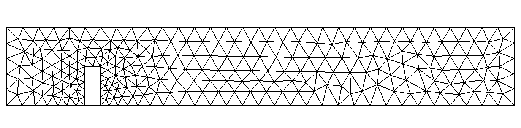
\includegraphics[width=0.7\textwidth]{orig.png}}
  \centerline{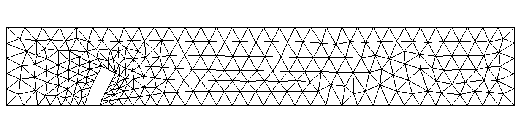
\includegraphics[width=0.7\textwidth]{deform.png}}
  \caption{The original computational mesh (up), and the mesh of the converged solution (down) of a FSI
    computation.}
\end{figure}

%\bibliography{elmerbib}
%\bibliographystyle{plain}


\graphicspath{{./}{helmholtzsolve/}}
\chapter{Helmholtz Solver}

\modinfo{Module name}{HelmholtzSolve}
\modinfo{Module subroutines}{\Idx{HelmholtzSolver}}
\modinfo{Module authors}{Juha Ruokolainen, Mikko Lyly}
\modinfo{Document authors}{Juha Ruokolainen}
\modinfo{Document edited}{March 30th 2006}

\section{Introduction}

This module solves the Helmholtz equation, which is the Fourier transform
of the wave equation. 

\section{Theory}

For example, sound propagation in air is fairly well described by the
wave equation:
\begin{equation}
\frac{1}{c^2}\frac{\partial^2 p}{\partial t^2} - \nabla^2p  = 0.
\end{equation}

When linear the equation may be written in frequency space as
\begin{equation}
k^2 P + \nabla^2P  = 0,
\end{equation}
where $k=\omega/c$.
This is the Helmholtz equation.
The instantaneous pressure may be computed
from the given field $P$:
\begin{equation}
p(t) = \Re(P e^{i\omega t}) = \Re(P)\cos(\omega t) - \Im(P)\sin(\omega t),
\end{equation}
where $i=\sqrt{-1}$ is the imaginary unity.

In Elmer  the equation has an added term which is proportional
to first time derivative of the field, whereupon the equation becomes
\begin{equation}
(k^2 - ikD)P + \nabla^2P  = 0,
\label{eq-sdamp}
\end{equation}
where $D$ is the damping factor.


\subsection{Boundary Conditions}

The usual boundary condition for the Helmholtz equation is to
give the flux on the boundary:
\begin{equation}
\nabla P\cdot\Vec{n} = g,
\end{equation}
also Dirichlet boundary conditions may be set.
The Sommerfeldt or far field boundary condition is as follows
\begin{equation}\label{Sommerfeldt-bc}
\nabla P\cdot\Vec{n} + \frac{i\omega}{Z}P = 0,
\end{equation}
where the complex-valued quantity $Z$ may be defined by the user.
It is noted that incoming and outgoing waves may be approximated by
setting $Z=\pm c$, respectively.
%the plus and minus describe incoming and outgoing waves respectively.


\section{Keywords} 

\sifbegin

\sifitem{Simulation}{}
This section gives values to parameters concerning the simulation
as whole.
\sifbegin
\sifitem{Frequency}{Real}
Give simulation frequency in units of $1/\mathrm{s}$.
Alternatively use the {\tt Angular Frequency} keyword.
\sifitem{Angular Frequency}{Real}
Give simulation frequency in units of $1/\mathrm{rad}$.
Alternatively use the {\tt Frequency} keyword.
\sifend

\sifitem{Solver}{solver id} 
Note that all the keywords related to linear solver (starting
with {\tt Linear System})
may be used in this solver as well.  They are defined elsewhere. 
Note also that for the Helmholtz equation {\tt ILUT} preconditioning
works well.

\sifbegin
\sifitem{Equation}{String [Helmholtz]} 
The name of the equation.
\sifitem{Procedure}{File ["HelmholtzSolve"\ "HelmholtzSolver"]}
This keyword is used to give the Elmer solver the place where
to search for the Helmholtz equation solver.
\sifitem{Variable}{String [Pressure]}
Give a name to the field variable.
\sifitem{Variable DOFs}{Integer [2]}
This keyword must be present, and {\it must} be set to the value $2$.
\sifitem{Bubbles}{Logical}
If set to {\tt True} this keyword activates the bubble stabilization.
\sifend

\sifitem{Equation}{eq id}
The equation section is used to define a set of equations for a body or set of bodies:
\sifbegin
\sifitem{Helmholtz}{Logical} If set to {\tt True}, solve the Helmholtz equation,
the name of the variable must match the {\tt Equation} setting in the {\tt Solver} section.
\sifend


\sifitem{Initial Condition}{ic id} 
The initial condition section may be used to set initial values for the field
variables. The following variables are active:
\sifbegin
\sifitem{Pressure i}{Real} 
For each the real and imaginary parts of the solved field {\tt i}$=1,2$.
\sifend

\sifitem{Material}{mat id}
The material section is used to give the material parameter values. The
following material parameters may be set in Helmholtz equation.
\sifbegin
\sifitem{Sound Speed}{Real} 
This keyword is use to give the value of the speed of sound.
\sifitem{Sound Damping}{Real} 
This keyword is use to give the value of the damping factor $D$ in
equation \ref{eq-sdamp}.
\sifend


\sifitem{Boundary Condition}{bc id}
The boundary condition section holds the parameter values for various
boundary condition types. Dirichlet boundary conditions may be
set for all the primary field variables. The one related to Helmholtz equations
are
\sifbegin
\sifitem{Pressure i}{Real} 
Dirichlet boundary condition
for real and imaginary parts of the variable.
Here the values {\tt i}$=1,2$ correspond to the real and 
imaginary parts of the unknown field.
\sifitem{Wave Flux 1,2}{Real}
Real and imaginary parts of the boundary flux.
Here the values {\tt i}$=1,2$ correspond to the real and 
imaginary parts of the boundary flux.
\sifitem{Wave Impedance 1,2}{Real}
This keyword may be used to define the real and imaginary parts of
the quantity $Z$ in (\ref{Sommerfeldt-bc}).
Here the values {\tt i}$=1,2$ correspond to the real and 
imaginary parts of $Z$.
%Real and imaginary parts of the boundary impedance {\tt i}$=1,2$.
%The impedance is used to compute the boundary wave number for the
%Sommerfeldt boundary condition:
%\begin{equation}
%k = \frac{\omega}{\mathrm{impedance}}.
%\end{equation}
\sifend
\sifend


%\bibliography{elmerbib}
%\bibliographystyle{plain}


\graphicspath{{./}{acoustics/}}
\include{acoustics/acoustics}

%\graphicspath{{./}{acoustics2/}}
%\include{acoustics2/segregated-solver}

\graphicspath{{./}{poissonbem/}}
\Chapter{BEM Solver for Poisson Equation}

\modinfo{Module name}{PoissonBEM}
\modinfo{Module subroutines}{\Idx{PoissonBEMSolver}}
\begin{versiona}
\modinfo{Module authors}{Juha Ruokolainen}
\modinfo{Document authors}{Juha Ruokolainen}
\modinfo{Document edited}{May 27th 2003}

\section{Introduction}

This module solves the Laplace equation by \Idx{boundary element method} (\Idx{BEM}), where
the differential equation is transformed to integral equation along the
boundaries. On the boundaries either potential or normal flux may be defined.
A source term may be included (Poisson equation), but the source term remains
a volume integral.

\section{Theory}

The Poisson equation is mathematically described as
\begin{equation}
-\Delta \Phi - f = 0, \mbox{ in } \Omega,
\end{equation}
where $f$ is the given source.

In BEM we transform this equation to \Idx{integral equation} over boundaries. We start
by multiplying the equation by a weight function and integrating over the volume,
and integrating by parts
\begin{equation}
-\int_\Omega \Delta \Phi w\ d\Omega  = \int_\Omega \nabla\Phi\cdot \nabla w\ d\Omega  -
\int_\Gamma \frac{\partial\Phi}{\partial n} w\ d\Gamma.
\end{equation}
Similarily we may write an equation reversing the roles of $\Phi$ and $w$
\begin{equation}
-\int_\Omega \Delta w \Phi\ d\Omega = \int_\Omega \nabla w\cdot \nabla \Phi\ d\Omega  -
\int_\Gamma \frac{\partial w}{\partial n} \Phi\ d\Gamma.
\end{equation}
Substracting the two equations we have
\begin{equation}
-\int_\Omega \Delta \Phi w\ d\Omega =
-\int_\Omega \Delta w \Phi\ d\Omega -
\int_\Gamma \frac{\partial\Phi}{\partial n} w\ d\Gamma +
\int_\Gamma \frac{\partial w}{\partial n} \Phi\ d\Gamma
\end{equation}
Next we choose the weight $w$ as follows:
\begin{equation}
-\Delta w = \delta_r(r'),
\end{equation}
so that 
\begin{equation}
-\int_\Omega \Delta w \Phi\ d\Omega = \Phi(r), 
\end{equation}
The weight $w$ chosen this way is the Green's function for the Laplace operator,
i.e.

\begin{equation}
 w(r,r') = \frac{\log(r-r')}{2\pi} \mbox{ in 2d }, 
 w(r,r') = \frac{1}{4\pi(r-r')} \mbox{ in 3d }.
\end{equation}

Finally we add the source term, and we have the equation
\begin{equation}
\Phi(r) -
\int_\Gamma \frac{\partial\Phi}{\partial n} w\ d\Gamma +
\int_\Gamma \frac{\partial w}{\partial n} \Phi\ d\Gamma - \int_\Omega fw\ d\Omega = 0.
\end{equation}
Only the source term is now integrated over the volume.
This equation may now be discretized by standard methods.

\subsection{Boundary Conditions}

Boundary conditions may be set for either potential
\begin{equation}
\Phi = \Phi_\Gamma \mbox{ on } \Gamma,
\end{equation}
or normal flux
\begin{equation}
-\frac{\partial \Phi}{\partial n} = g \mbox{ on } \Gamma.
\end{equation}



\section{Keywords} 
\end{versiona}

\sifbegin

\sifitem{Solver}{solver id} 
Note that all the keywords related to linear solver (starting with {\tt Linear System})
may be used in this solver as well.
They are defined elsewhere.  Note also that the BEM discretization
results to a full linear system in contrast to FEM discretizations
and the ILU preconditioning settings are not available.

\sifbegin
\sifitem{Equation}{String [PoissonBEM]} 
The name of the equation.
\sifitem{Procedure}{File ["PoissonBEM"\ "PoissonBEMSolver"]}
This keyword is used to give the Elmer solver the place where
to search for the  equation solver.
\sifitem{Variable}{String [Potential]}
Give a name to the field variable.
\sifitem{Variable DOFs}{Integer [1]}
This keyword must be present, and {\it must} be set to the value $1$.
\sifitem{Exported Variable 1}{String Flux}
If this keyword is given, the output will include the normal flux at
boundaries, the name must be exactly as given.
\sifitem{Exported Variable 1 DOFs}{Integer [1]}
This keyword must be present if Flux values are to be computed,
and {\it must} be set to the value $1$.
\sifend

\sifitem{Equation}{eq id}
The equation section is used to define a set of equations for a body or set of bodies:
\sifbegin
\sifitem{PoissonBEM}{Logical} if set to {\tt True}, solve the Poisson equation,
the name of this parameter must match the {\tt Equation} setting in the {\tt Solver} section.
\sifend
If the mesh has any volume elements with a body id that corresponds to a body where to
the Poisson equation is activated, the value of the potential is computed for these elements
as a postprocessing step. Note that the computation of potential is not a trivial task,
so large number of volume elements may result to long execution time.

\sifitem{Boundary Condition}{bc id}
The boundary condition section holds the parameter values for various
boundary condition types. Dirichlet boundary conditions may be
set for all the primary field variables. The one related to Poisson (BEM) equation
are
\sifbegin
\sifitem{Body Id}{Integer}
Give body identification number for this boundary, used to reference
body definitions in .sif file. This parameter must be set so that the ElmerSolver
knows at which boundaries to solve the corresponding equation.
\sifitem{Potential}{Real} 
Known potential value at boundary.
\sifitem{Flux}{Real}
Known normal flux at boundary.
\sifitem{Normal Target Body}{Integer}
The direction of boundary normals are important for the success of the computation. They
should point consistently outward from the boundaries. This is accomplished either if
the mesh generator automatically orients the boundary elements consistently, or including
in the mesh the parent (volume) elements of the boundaries and using this keyword. The value
-1 of this parameter points to the side where there are no volume elements. If the parameter
gets the value of the body id of the volume elements, the normal will point to that direction.
\sifend

\sifitem{Body Force}{bf id}
The source term for the Poisson equation may be given here. The volume integral
is computed on a body with a volume mesh and the PoissonBEM equation set to true.
\sifbegin
\sifitem{Source}{Real}
The source term for the Poisson equation.
\sifend
\sifend


%\bibliography{elmerbib}
%\bibliographystyle{plain}



\graphicspath{{./}{helmholtzbem/}}
\chapter{BEM Solver for Helmholtz Equation}

\modinfo{Module name}{HelmholtzBEM}
\modinfo{Module subroutines}{\Idx{HelmholtzBEMSolver}}
\begin{versiona}
\modinfo{Module authors}{Juha Ruokolainen}
\modinfo{Document authors}{Juha Ruokolainen}
\modinfo{Document edited}{May 27th 2003}

\section{Introduction}

This module solves the Helmholtz equation by \Idx{boundary element method} (\Idx{BEM}), where
the differential equation is transformed to \Idx{integral equation} along the
boundaries. On the boundaries either pressure or normal flux may be defined.

\section{Theory}

The Helmholtz equation is mathematically described as
\begin{equation}
(k^2+\Delta ) \Phi  = 0, \mbox{ in } \Omega.
\end{equation}

In BEM we transform this equation to integral equation over boundaries. We start
by multiplying the equation by a weight function and integrating over the volume,
and integrating by parts
\begin{equation}
\int_\Omega (k^2+\Delta \Phi) w\ d\Omega  =
\int_\Omega k^2 w\Phi d\Omega -
\int_\Omega \nabla\Phi\cdot \nabla w\ d\Omega +
\int_\Gamma \frac{\partial\Phi}{\partial n} w\ d\Gamma.
\end{equation}
Similarily we may write an equation reversing the roles of $\Phi$ and $w$
\begin{equation}
\int_\Omega (k^2+\Delta) w \Phi\ d\Omega =
\int_\Omega k^2 w\Phi d\Omega -
\int_\Omega \nabla w\cdot \nabla \Phi\ d\Omega  +
\int_\Gamma \frac{\partial w}{\partial n} \Phi\ d\Gamma.
\end{equation}
Substracting the two equations we have
\begin{equation}
\int_\Omega (k^2+\Delta) \Phi w\ d\Omega =
\int_\Omega (k^2+\Delta) w \Phi\ d\Omega -
\int_\Gamma \frac{\partial\Phi}{\partial n} w\ d\Gamma +
\int_\Gamma \frac{\partial w}{\partial n} \Phi\ d\Gamma
\end{equation}
Next we choose the weight $w$ as follows:
\begin{equation}
(k^2+\Delta)w = \delta_r(r'),
\end{equation}
so that 
\begin{equation}
\int_\Omega (k^2+\Delta) w \Phi\ d\Omega = \Phi(r), 
\end{equation}
The weight $w$ chosen this way is the \Idx{Green's function} for the Helmholtz operator,
i.e.

\begin{equation}
 w(r,r') = \frac{1}{i4}H_0(k(r-r')) \mbox{ in 2d }, 
 w(r,r') = \frac{1}{4\pi}\exp^{-ik(r-r')} \mbox{ in 3d },
\end{equation}
where $H_0$ is the Hankel function.

Finally we have the equation
\begin{equation}
\Phi(r) -
\int_\Gamma \frac{\partial\Phi}{\partial n} w\ d\Gamma +
\int_\Gamma \frac{\partial w}{\partial n} \Phi\ d\Gamma = 0.
\end{equation}

\subsection{Boundary Conditions}

Boundary conditions may be set for either pressure
\begin{equation}
\Phi = \Phi_\Gamma \mbox{ on } \Gamma,
\end{equation}
or normal flux
\begin{equation}
-\frac{\partial \Phi}{\partial n} = g \mbox{ on } \Gamma.
\end{equation}


\section{Keywords} 
\end{versiona}

\sifbegin

\sifitem{Simulation}{}
\sifbegin
\sifitem{Angular Frequency}{Real}
Give the value of the angular frequency for the simulation.
\sifend

\sifitem{Solver}{solver id} 
Note that all the keywords related to linear solver (starting with {\tt Linear System})
may be used in this solver as well.
They are defined elsewhere.  Note also that the BEM discretization
results to a full linear system in contrast to FEM discretizations
and the ILU preconditioning settings are not available.

\sifbegin
\sifitem{Equation}{String [HelmholtzBEM]} 
The name of the equation.
\sifitem{Procedure}{File ["HelmholtzBEM"\ "HelmholtzBEMSolver"]}
This keyword is used to give the Elmer solver the place where
to search for the  equation solver.
\sifitem{Variable}{String [Pressure]}
Give a name to the field variable.
\sifitem{Variable DOFs}{Integer [2]}
This keyword must be present, and {\it must} be set to the value $2$.
\sifitem{Exported Variable 1}{String Flux}
If this keyword is given, the output will include the normal flux at
boundaries, the name must be exactly as given.
\sifitem{Exported Variable 1 DOFs}{Integer [2]}
This keyword must be present if Flux values are to be computed,
and {\it must} be set to the value $2$.
\sifend

\sifitem{Equation}{eq id}
The equation section is used to define a set of equations for a body or set of bodies:
\sifbegin
\sifitem{HelmholtzBEM}{Logical} if set to {\tt True}, solve the Helmholtz equation,
the name of this parameter must match the {\tt Equation} setting in the {\tt Solver} section.
\sifend
If the mesh has any volume elements with a body id that corresponds to a body where to
the Helmholtz equation is activated, the value of the pressure is computed for these elements
as a postprocessing step. Note that the computation of potential is not a trivial task,
so large number of volume elements may result to long execution time.

\sifitem{Boundary Condition}{bc id}
The boundary condition section holds the parameter values for various
boundary condition types. Dirichlet boundary conditions may be
set for all the primary field variables. The one related to Helmholtz (BEM) equation
are
\sifbegin
\sifitem{Body Id}{Integer}
Give body identification number for this boundary, used to reference
body definitions in .sif file. This parameter must be set so that the ElmerSolver
knows at which boundaries to solve the corresponding equation.
\sifitem{Pressure 1}{Real} 
Known real part of pressure at boundary.
\sifitem{Pressure 2}{Real} 
Known imaginary part of pressure at boundary.
\sifitem{Flux 1}{Real}
Known real part of normal flux at boundary.
\sifitem{Flux 2}{Real}
Known real part of normal flux at boundary.
\sifitem{Normal Taget Body}{Integer}
The direction of boundary normals are important for the success of the computation. They
should point consistently outward from the boundaries. This is accomplished either if
the mesh generator automatically orients the boundary elements consistently, or including
in the mesh the parent (volume) elements of the boundaries and using this keyword. The value
-1 of this parameter points to the side where there are no volume elements. If the parameter
gets the value of the body id of the volume elements, the normal will point to that direction.
\sifend

\sifend


%\bibliography{elmerbib}
%\bibliographystyle{plain}



%\graphicspath{{./}{navier-stokes/}}
%\include{PorousFlow/PorousFlow}

\graphicspath{{./}{electrostatics/}}
\chapter{Electrostatics}

\modinfo{Directory}{\Idx{Electrostatics}}
\modinfo{Solvers}{\Idx{StatElecSolve}, \Idx{ElectricForce}}
\modinfo{Tools}{\Idx{ElmerGrid}, editor}
\modinfo{Dimensions}{3D, Steady-state}

\subsection*{Case definition}

This case presents solving the Poisson equation for electric potential
and calculating appropriate derived quantities, such as
\Idx{capacitance}, based on the result. The geometry studied is a
symmetric quadrant of a plane capacitor having a rectangular hole in
another plate. A setting of this kind can be used to study the effects
of geometrical features on the capacitance and on the electrostatic
force, which both are meaningful quantities for coupled
simulations in {\em e.g.}  microsystems.


\subsection*{Solution procedure}

The mesh is constructed using ElmerGrid with the following command
\ttbegin
ElmerGrid 1 2 elmesh.grd
\ttend
The mesh is extended above the hole to avoid undesired boundary
effects. The geometry is presented in the Figure~\ref{geo_elstat}

\begin{figure}[hbt]
  \centerline{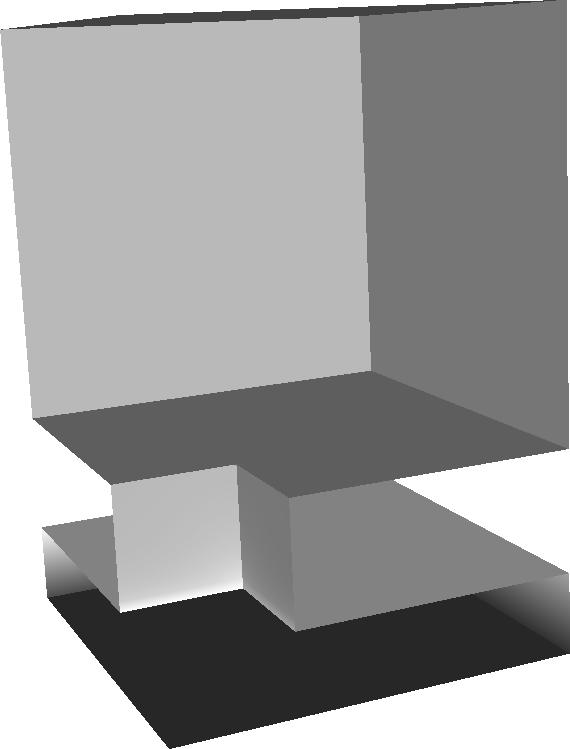
\includegraphics[width=0.32\textwidth]{geo_elstat}}
  \caption{The geometry of problem.} 
  \label{geo_elstat}
\end{figure}

The simulation problem includes a single body, and thus one material
and one equation set, as well as three solvers. The solvers are used
to compute the electric potential and related quantities, to calculate
the electric force, and to save relevant data into a file. This
tutorial is defined in Elmer \Idx{MEMS} units. The sif-file is presented
below.

\ttbegin
Check Keywords Warn

Header
  Mesh DB "." "elmesh"
End
\ttend

Only a single steady state iteration is needed, since the Poisson
equation is linear.
\ttbegin
Simulation
  Coordinate System = Cartesian 3D
  Simulation Type = Steady State
  Steady State Max Iterations = 1
  Output File = "elstatics.result"
  Post File = "elstatics.ep"
End
\ttend

The permittivity of vacuum has to be defined in the Constants section.
\ttbegin
Constants
  Permittivity Of Vacuum = 8.8542e-12
End

Body 1
  Equation = 1
  Material = 1
End
\ttend

Electric energy density is added into the results in Equation
section. This allows energy density to be visualised in
ElmerPost. Note also, that calculating electric flux (or the electric
displacement field) is disabled in the Solver~1 block. Further, the
potential difference used in calculating the capacitance of the system
has to be defined in this section. This should be the same as the
boundary conditions define for the capacitance calculation to be
sensible.
\ttbegin
Equation 1
  Active Solvers(2) = 1 2
  Calculate Electric Energy = True  ! (default False)
End

Solver 1
  Equation = Stat Elec Solver
  Variable = Potential
  Variable DOFs = 1
  Procedure = "StatElecSolve" "StatElecSolver"
  Calculate Electric Field = True  ! (default True)
  Calculate Electric Flux = False  ! (default True)
  Potential Difference = 1.0e6
  Linear System Solver = Iterative
  Linear System Iterative Method = BiCGStab
  Linear System Max Iterations = 200
  Linear System Convergence Tolerance = 1.0e-07
  Linear System Preconditioning = ILU1
  Linear System ILUT Tolerance = 1.0e-03
  Nonlinear System Max Iterations = 1
  Nonlinear System Convergence Tolerance = 1.0e-4
  Nonlinear System Newton After Tolerance = 1.0e-3
  Nonlinear System Newton After Iterations = 10
  Nonlinear System Relaxation Factor = 1
  Steady State Convergence Tolerance = 1.0e-4
End
\ttend

The static electric force solver does not need a lot of
information:
\ttbegin
Solver 2
  Equation = Electric Force
  Procedure = "ElectricForce" "StatElecForce"
End
\ttend

Finally, some data is saved in file scalars.dat in working directory.
\ttbegin
Solver 3
  Exec Solver = After All
  Equation = SaveScalars
  Procedure = "\Idx{SaveData}" "SaveScalars"
  Filename = "scalars.dat"
End
\ttend

Only the relative permittivity of the material has to be defined.
\ttbegin
Material 1
  Relative Permittivity = 1
End
\ttend

The boundary conditions include the values of electric potential
(voltage) and indication on which boundary the electric force should
be calculated. On all the other boundaries a natural boundary
condition is used, basically stating that the electric flux through
these boundaries is zero.
\ttbegin
Boundary Condition 1
  Target Boundaries = 4
  Potential = 0.0
  Calculate Electric Force = True
End

Boundary Condition 2
  Target Boundaries = 3
  Potential = 1.0e6
End
\ttend


\subsection*{Results}

The results obtained for capacitance and electric force are compared
to those of a complete plane capacitor. For a plane capacitor, the
capacitance is
\begin{equation}
C=\varepsilon_r\varepsilon_0\frac{A}{d},
\end{equation}
and the electrostatic force is
\begin{equation}
F_e = \frac{1}{2}\varepsilon_r\varepsilon_0\frac{A}{d^2}\Phi^2,
\end{equation}
where $\varepsilon_r$ is the relative permittivity, $\varepsilon_0$
is the permittivity of vacuum, $A$ is the area of a capacitor plate,
$d$ is the separation of the capacitor plates, and $\Phi$ is the
potential difference between the plates.

The results of the simulation as well as the comparison to the
complete plane capacitor values are shown in Table~\ref{tab_elstatics}
(in Elmer MEMS units). Note that the fringe fields on capacitor edges
are not calculated. This would require much larger mesh extending
outside the capacitor boundaries.

\begin{table}[htb]
\caption{Comparison of numerical results to analytic values}
\label{tab_elstatics}
\begin{center}
\begin{tabular}{lccc} \hline
            & simulation & analytic & ratio \\ \hline
Capacitance & \ \ $2.1361\cdot 10^{-10}$\ \  & 
              \ \ $2.2136\cdot 10^{-10}$\ \  & 0.965 \\
Electric Force & $1.0406\cdot 10^2$ & 
                 $1.1068\cdot 10^2$ & 0.940 \\ \hline
\end{tabular}
\end{center}
\end{table}

Finally, a picture of the results is presented. The
Figure~\ref{res_elstat} shows the isosurfaces of the electric
potential with the color marking the strength of the electric
field. From the picture it is clearly seen that the electric field is
constant between the plates except for the proximity of the hole which
causes weakening of the field magnitude. There are also strong
electric fields at the edges of the hole.


\begin{figure}[hbt]
  \centerline{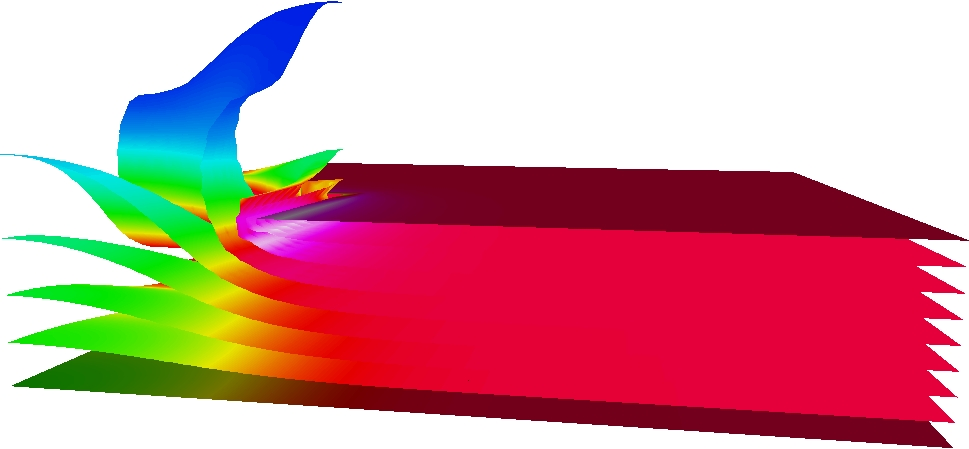
\includegraphics[width=0.8\textwidth]{res_elstat}}
  \caption{Isosurfaces of the potential coloured with electric field
  magnitude.} 
  \label{res_elstat}
\end{figure}



\vfill
\mbox{}



\graphicspath{{./}{statcurrent/}}
\Chapter{Static Current Conduction}\label{chap:statcurr}

\modinfo{Module name}{\Idx{StatCurrentSolve}}
\modinfo{Module subroutines}{\Idx{StatCurrentSolver}}

\begin{versiona}
\modinfo{Module authors}{Leila Puska, Antti Pursula, Peter R�back}
\modinfo{Document authors}{Antti Pursula}
\modinfo{Document edited}{August 2nd 2002}


\section{Introduction}

The macroscopic electromagnetic theory is governed by the Maxwell's
equations. This module solves the electrostatic potential in
conducting medium allowing volume currents and electric power loss
(Joule heating) to be derived.


\section{Theory}

In quasi-static approximation, when $\varepsilon \mu c^2 << 1$, the
first and fourth Maxwell equation can be written as follows
\begin{eqnarray}
\nabla\cdot \Vec{D} & = & \rho \label{max1} \\
%\nabla\cdot \Vec{B} & = & 0 \\
%\nabla\times \Vec{E} & = & -\frac{\partial\Vec{B}}{\partial t} \\
\nabla\times \Vec{H} & = & \Vec{J} + \frac{\partial\Vec{D}}{\partial t}
\label{max4}
\end{eqnarray}

The continuity equation for electric charges is
easily derived from the above Maxwell Eqs.~\ref{max1} and~\ref{max4}
\begin{equation}
\frac{\partial \rho}{\partial t} + \nabla\cdot \Vec{J} = 0
\label{elcontinuity}
\end{equation}
The \Idx{Ohm's law} for conducting material gives
the relationship between \Idx{current density} and 
electric field,
\begin{equation}
\Vec{J} = \sigma \Vec{E}
\label{ohm}
\end{equation}
In steady-state case the electric field may be expressed with a help of
an electric scalar potential $\phi$, 
\begin{equation}
\Vec{E} = -\nabla \phi . 
\label{elpot}
\end{equation}

Starting from the continuity equation~\ref{elcontinuity} and using
Eqs.~\ref{ohm} and~\ref{elpot} we get
\begin{equation}
\nabla\cdot\sigma\nabla\phi = \frac{\partial\rho}{\partial t}.
\end{equation}
This Poisson equation is used to solve the electric potential. The
source term is often zero but in some cases it might be necessary.

The volume current density is now calculated by
\begin{equation}
\vec{J} = -\sigma\nabla\phi,
\end{equation}
and electric power loss density which is turned into heat by
\begin{equation}
h = \nabla\phi\cdot\sigma\nabla\phi.
\end{equation}
The latter is often called the \Idx{Joule heating}. The total heating power
is found by integrating the above equation over the conducting
volume.

\subsection{Boundary Conditions}

For electric potential either Dirichlet or Neumann boundary condition
can be used. The Dirichlet boundary condition gives the value of the
potential on specified boundaries. The Neumann boundary condition is
used to give a current $J_b$ on specified boundaries
\begin{equation}
J_b = \sigma\nabla\phi\cdot\vec{n}.
\end{equation}


\subsection{Power and current control}

Sometimes the desired power or corrent of the system is known a priori.
The control may be applied to the system.
When the electric potential has been computed the heating power may be estimated from
\begin{equation}
 P = \int_\Omega \nabla \phi \cdot \sigma\nabla\phi \, d\Omega .
\end{equation}
If there is a potential difference $U$ in the system the effective resistance may also be
computed from $R=U^2/P$ and the effective current from $I=P/U$. 

The control is achieved by multiplying the potential and all derived field by a suitable variable.
For power control the coefficient is 
\begin{equation}
  C_P = \sqrt{ P_0 / P },
\end{equation}
where $P_0$ is the desired power. For current control the coefficient is 
\begin{equation}
  C_I = I_0 / I,
\end{equation}
where $I_0$ is the desired total current.




\section{Note on output control}

The user can control which derived quantities ({\em i.e.} volume
current and Joule heating) are calculated and additionally specify if
he/she wants to output also the electric conductivity. The latter is
useful when the conductivity depends for example on temperature. This
feature is available only for isotropic (scalar) conductivities.

There are also available two choises of visualization types for the
derived quantities. The node values can be calculated by taking the
average of the derived values on neighbouring elements (constant
weights). This results often in visually good images. The other
possible choice is to weight the average with the size of the
elements, which is more accurate and should be used when some other
variable depends on these derived values. The latter choice is also
the default.


\section{Keywords}
\end{versiona}

\sifbegin
\sifitemnt{Solver}{solver id}
\sifbegin
\sifitemnt{Equation}{String Stat Current Solver}
\sifitem{Variable}{String Potential}
This may be of any name as far as it is used consistently also elsewhere.
\sifitem{Variable DOFs}{Integer 1}
Degrees of freedom for the potential.
\sifitem{Procedure}{File "StatCurrentSolve"\ "StatCurrentSolver"}
Following are listed three keywords with default values
for output control.
\sifitemnt{Calculate Volume Current}{Logical [True]}
\sifitemnt{Calculate Joule Heating}{Logical [True]}
\sifitem{Constant Weights}{Logical [True]}
Used to turn constant weighting on for the results.
\sifitem{Power Control}{Real} 
Apply power control with the desired heating power being $P_0$.
\sifitem{Current Control}{Real} 
Apply current control with the desired current being $I_0$.
\sifend

\sifitemnt{Material}{mat id}
\sifbegin
\sifitemnt{Electric Conductivity}{Real}
\sifend

\sifitemnt{Body Force}{bodyforce id}
\sifbegin
\sifitem{Current Source}{Real}
Possibility for a current source, not used often though.
\sifitem{Joule Heat}{Logical}
If this flag is active the Heat equation will automatically compute the 
quantity $\nabla \phi \cdot \sigma\nabla\phi$ as heat source.
Then it is assumed that $\phi$ is named \texttt{Potential}.
If there is no heat equation this flag has no effect.
\sifend

\sifitemnt{Boundary Condition}{bc id}
\sifbegin
\sifitem{Potential}{Real}
Dirichlet BC for the potential.
\sifitem{Current Density BC}{Logical}
Must be set to {\tt True} if Neumann BC is used.
\sifitem{Current Density}{Real}
Neumann boundary condition for the current.
\sifend
\sifend

\begin{versiona}
\bibliography{elmerbib}
\bibliographystyle{plain}
\end{versiona}



\graphicspath{{./}{magnetostatics/}}
\include{magnetostatics/vectorpotential}

\graphicspath{{./}{mhd/}}
\include{mhd/induction}

\graphicspath{{./}{electrokinetics/}}
\chapter{\Idx{Electrokinetics}}
\noindent
\modinfo{Module name}{\Idx{Electrokinetics}}
\modinfo{Module subroutines}{helmholtz\_smoluchowski1, helmholtz\_smoluchowski2,\\ helmholtz\_smoluchowski3, helmholtz\_smoluchowski, getJouleHeat}
\begin{versiona}
\modinfo{Module author}{Thomas Zwinger}
\modinfo{Document author}{Thomas Zwinger}
\modinfo{Document created}{April 13th 2005}

\section{Introduction}

If dealing with electrolytic fluids constrained to small volumes, surface forces caused by electric surface charges in combination with externally applied electrostatic fields are sufficient strong to affect the fluid volume. If these effects are utilized to attenuate the fluid volume, we talk of \textit{Electrokinetics}. The term \textit{Electroosmotic Flow} (EOF) is used in connection with the attenuation of a net charge inside a originally neutral electrolyte caused by separation induced by a surface charge of a wall.

In most applications utilizing EOF, externally applied fields are sufficient small in order to justify neglecting electric heating (Joule heating) inside the fluid volume. Nevertheless, certain applications, such as High Voltage Capillary Electrophoresis (HV-CE), demand the consideration of this effect \cite{KnoMcC1994}.

\section{Theory}
Chemical reactions between the contents of a liquid and the wall material may lead to a net charge of the containment at the wall-liquid interface. If the liquid is an electrolyte (i.e., it contains free ions), ions of opposite charge align along the wall creating the \textit{Stern layer}. Adjacent to the Stern layer, a charge separation - called the \textit{diffuse layer} of the initially neutral electrolyte takes place. Due to the two layer structure the whole are area of charge separation in the vicinity of a wall is called the \textit{Electric Double layer} (EDL). 
\begin{figure}[tbhp]
%\vspace{-11cm}
\centerline{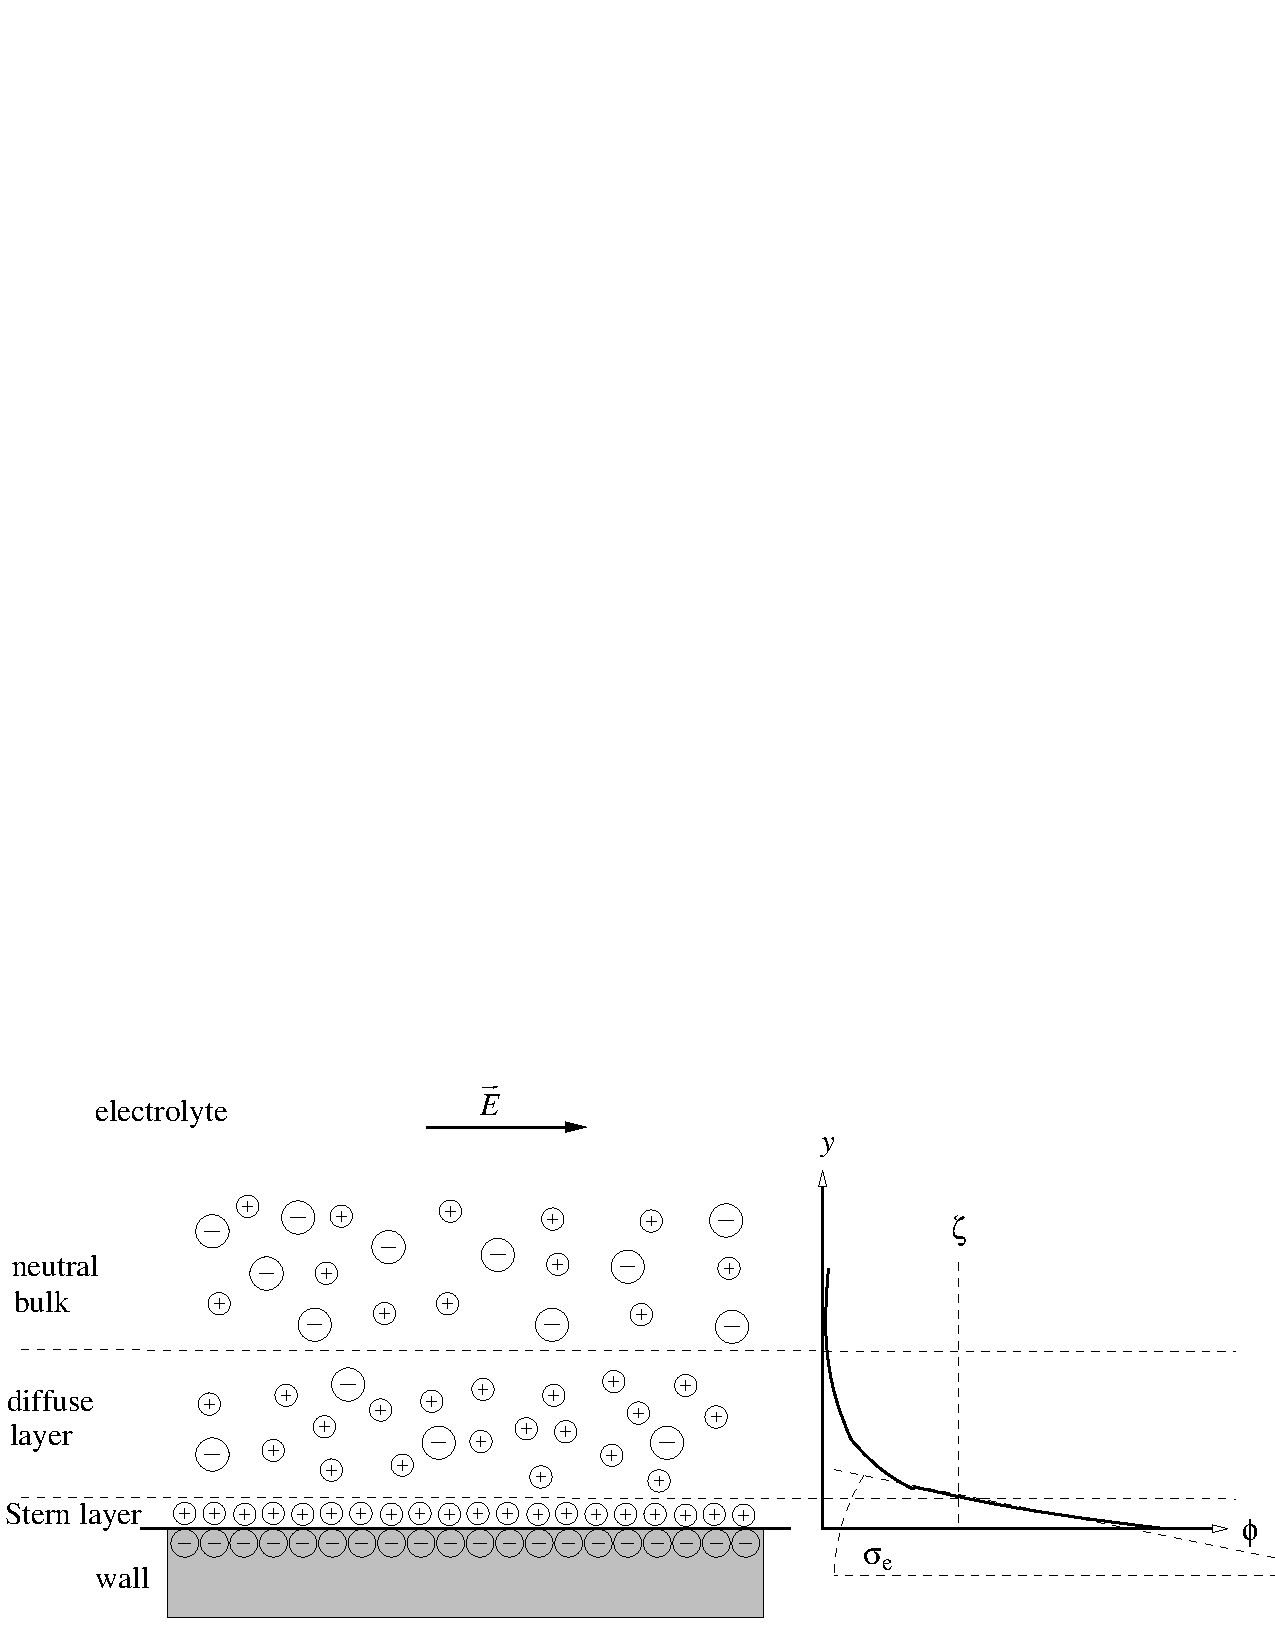
\includegraphics[width=0.9\textwidth]{EDL_bw.pdf}}
\caption{\label{ek:Fig.EDL} Structure of the EDL. The value of the induced potential, $\Phi$ at the Stern layer usually is referred to as the zeta-potential, $\zeta$}
\end{figure}
\subsection{Electroosmotic slip velocity}\label{EOF}
Considering a symmetric electrolyte -- i.e., the bulk ion density of ions with opposite valence numbers $\pm z$ are equal $n^{+}_{0}=n^{-}_{0}=n_{0}$ --  at a certain temperature, $T$, the typical width-scale of the EDL is given by the \textit{Debye length} \cite{KarBes:2001}
\begin{equation}\label{ek:debye}
\lambda_{\mathrm{D}} = \left(\dfrac{\epsilon_{\mathrm{f}}\epsilon_{0}\,k_{\mathrm{b}}\,T_{0}}{2\, n_{0}\, z^{2}\, e^{2}_{0} }\right)^{1/2}.
\end{equation}
Here $e_{0}$ stands for the unit charge and $k_{\mathrm{b}}$ denotes the Boltzmann constant. The relative permittivity of the electrolyte and the permittivity of vacuum are given by $\epsilon_{\mathrm{f}}$ and $\epsilon_{0}$, respectively. 


The potential, $\Phi$ and the volume charge density, $\rho_{e}$, within the EDL are tightly coupled to each other by the Poisson-Boltzmann equation \eqref{eq:poisson-boltzmann} (see chapter \ref{poisson-boltzmann}). In order to exactly resolve the dynamics close to the walls, \eqref{eq:poisson-boltzmann} should be solved and the resulting specific electric force then be considered in the equation of motion. Nevertheless,  provided the typical length scales of the flow perpendicular to the containment walls, $H$, strongly exceed those of the EDL -- in other words, we obtain very small values for the non-dimensional group $\mathcal{L} = \lambda_{\mathrm{D}}/H \ll 1$ -- the dynamics of the electrolyte inside the EDL does not have to be resolved at all. In this case simple considerations of a force balance between shear stress and electric force lead to a slip condition for the fluid \cite{YaFuLi:2001}. At the boundary, the tangential velocity is set to the \textit{Helmholtz-Smoluchowski} velocity
\begin{equation}
\label{ek:helm-smol}
\vec{u}_{\mathrm{tang.}}=\vec{u}_{\mathrm{H-S}} = \frac{\vec{E}_{\mathrm{tang.}}\epsilon_{\mathrm{f}}\epsilon_{0}\zeta}{\mu_{\mathrm{f}}},
\end{equation}
with $\mu_{\mathrm{f}}$ standing for the local fluid viscosity. The \textit{zeta potential}, $\zeta$ -- a property depending on the electric properties of the wall material as well as the electrolyte -- usually is determined experimentally. From a physical point of view it can be interpreted as the value of the solution obtained by \eqref{eq:poisson-boltzmann} at the Stern layer. The tangential component, $\vec{E}_{\mathrm{tang.}}$,  of the external electric field, $\vec{E}$, is evaluated from the outward pointing surface normal $\vec{n}$, applying the following relation
\begin{equation}
\label{ek:etang}
\vec{E}_{\mathrm{tang.}} = \vec{E} - \left(\vec{E}\cdot\vec{n}\right)\vec{n}
\end{equation}
Alternatively, the resulting slip velocity may be related to the tangential field using the \textit{Electroosmotic Mobility}, $\mu_{\mathrm{EOF}}$
\begin{equation}
\label{ek:HS-EOF-mobility}
\vec{u}_{\mathrm{H-S}} = \mu_{\mathrm{EO}}\,\vec{E}_{\mathrm{tang.}}.
\end{equation}
A combination of \eqref{ek:helm-smol} and \eqref{ek:HS-EOF-mobility} leads to the following identity
\begin{equation}
\label{ek:EOF-mobility}
\mu_{\mathrm{EO}} =\frac{\epsilon_{\mathrm{f}}\epsilon_{0}\zeta}{\mu_{\mathrm{f}}}.
\end{equation}

\subsection{Joule Heating}
Due to the small volume in microfluidic applications the additional heat produced by the external electric field needs to be considered. With the local electric conductivity, $\sigma$, and the local volume density, $\rho$, of the electrolyte the specific heat contribution by Joule heating from an external electric field, $\vec{E}$, is given by
\begin{equation}
\label{ek:joule-heating}
h = \sigma\,\vec{E}\cdot\vec{E}/\rho.
\end{equation}
The expression above can be added as body force to the heat transfer equation \eqref{heat_equation}.

\section{Limitations}
\begin{itemize}
\item The Helmholtz-Smoluchowski velocity should not be applied if the non-di\-men\-sion\-al group $\mathcal{L}$ defined in \ref{EOF} is of unity order or larger. Then the potential- and charge density distribution as well as the dynamics of the electrolyte inside the EDL has to be resolved. 
\item In a strict sense, the Helmholtz-Smoluchowski theory applies only to configurations where the normal-component of the external field, $\vec{E}\cdot\vec{n}$, is small. If dealing with electric insulating wall materials -- as it is usually the case in microfluidic applications -- this condition is implicitly complied with. 
\item The assumption of a Newtonian fluid underlies the derivation of the Helmholtz-Smoluchowski velocity.
\item The function \texttt{helmholtz\_smoluchowski} can only be applied on  boundaries of two-dimensional domains, where the tangential direction is uniquely defined.
\item The functions \texttt{helmholtz\_smoluchowski\{1,2,3\}} cannot be applied with a number larger than the dimension of the domain.
\end{itemize}


\section{Keywords}
\end{versiona}

\subsection*{Keywords for helmholtz\_smoluchowski}

\sifbegin

  \sifitemnt{Constants}{}
  \sifbegin
  \sifitem{Permittivity Of Vacuum}{Real [8.8542e-12 C$^2$/Nm$^2$]}
   permittivity of vacuum, only needed if Helmholtz-Smoluchowski velocity is defined using expression \eqref{ek:helm-smol}
  \sifend

  \sifitemnt{Equation}{equation id}
  \sifbegin
    \sifitem{Electric Field }{String  [\texttt{computed}, \texttt{\tt constant}]} 
    the option for how to evaluate the electric field should be set to one of these values.\newline
    If set to  \texttt{computed}, the function will search for \texttt{Electric Field \{1,2,3\}} in the list of solver variables. If set to \texttt{constant}, the function will search for \texttt{Electric Field \{1,2,3\}} in the section \texttt{Material material id}, where \texttt{material id} is the id-number associated with the material parameter list of the electrolyte
  \sifend

  \sifitemnt{Material}{material id} \newline
  If the Helmholtz-Smoluchowski velocity is defined using expression \eqref{ek:helm-smol}, then the following keywords have to be provided in this section
  \sifbegin
   \sifitem{Viscosity}{Real}
   viscosity of the electrolyte
   \sifitem{Density}{Real}
  volumetric density of the electrolyte
   \sifitem{Relative Permittivity}{Real}
   relative permittivity of the electrolyte
  \sifend
%   Alternatively, the user can declare the EO-mobility, as explained in \eqref{ek:EOF-mobility}

  \sifitemnt{Boundary Condition}{bc id} \newline
  In two-dimensional configurations the Helmholtz-Smoluchowski velocity directly can be assigned to the tangential component of the velocity field
  \sifbegin
    \sifitemnt{Normal Tangential Velocity}{Logical True}
    \sifitem{Velocity 2}{= Variable Dummyargument\\ Real Procedure "Electrokinetics"\ "helmholtz\_smolu\-chowski"}
          Sets tangential EO slip velocity
  \sifend
  The argument \texttt{Dummyargument} can be any existing variable, since it is not used to evaluate the velocity.\newline
  In three-dimensional configurations (and as an alternative also in two-dimensional), the velocity has to be defined for each component
  \sifbegin
    \sifitemnt{Normal Tangential Velocity}{Logical False} 
    \sifitemnt{Velocity 1}{= Variable Dummyargument\\ Real Procedure "Electrokinetics"\ "helmholtz\_smolu\-chowski1"}
    \sifitemnt{Velocity 2}{= Variable Dummyargument\\ Real Procedure "Electrokinetics"\ "helmholtz\_smolu\-chowski2"}
    \sifitemnt{Velocity 3}{= Variable Dummyargument\\ Real Procedure "Electrokinetics"\ "helmholtz\_smolu\-chowski3"}
  \sifend
  The argument \texttt{Dummyargument} can be any existing variable, since it is not used to evaluate the velocity.\newline
  If the Helmholtz-Smoluchowski velocity is defined using expression \eqref{ek:helm-smol}, then the zeta potential, $\zeta$, for the specific boundary region has to be defined
  \sifbegin
    \sifitem{Zeta Potential}{Real}
    Sets the zeta-potential for this boundary
  \sifend
  Alternatively, the user can declare the EO-mobility, as explained in \eqref{ek:EOF-mobility}
    \sifbegin
    \sifitem{EO Mobility}{Real}
        Sets EO mobility for this boundary
  \sifend
\sifend
\subsection*{Keywords for getJouleHeat}
\sifbegin
  \sifitemnt{Equation}{equation id}
  \sifbegin
    \sifitem{Electric Field }{String  [\texttt{computed}, \texttt{constant}]} 
    the option for how to evaluate the electric field should be set to one of these values.\newline
    If set to  \texttt{computed}, the function will search for \texttt{Electric Field \{1,2,3\}} in the list of solver variables. If set to \texttt{constant}, the function will search for \texttt{Electric Field \{1,2,3\}} in the section \texttt{Material material id}, where \texttt{material id} is the id-number associated with the material parameter list of the electrolyte
  \sifend

  \sifitemnt{Material}{material id}
   \sifbegin
    \sifitem{Electric Conductivity}{Real}
     electric conductivity of the electrolyte
    \sifitem{Density}{Real}
     volumetric density of the electrolyte
   \sifend

  \sifitemnt{Body Force}{bodyforce id}
   \sifbegin
    \sifitem{Heat Source}{= Variable Dummyargument \\ Real Procedure "Electrokinetics"\ "getJouleHeat"}
     adds specific heat source for \texttt{HeatSolve}.  
     The argument \texttt{Dummyargument} can be any existing variable, since it is not used to evaluate the Joule heating	
   \sifend
\sifend


\begin{versiona}
\bibliography{elmerbib}
\bibliographystyle{plain}
\end{versiona}




\graphicspath{{./}{PoissonBoltzmann/}}
\chapter{Poisson-Boltzmann Equation}\label{poisson-boltzmann}

\modinfo{Module name}{\Idx{PoissonBoltzmannSolve}}
\modinfo{Module subroutines}{PoissonBoltzmannSolve}
\modinfo{Module authors}{Peter R�back}
\modinfo{Document authors}{Peter R�back}
\modinfo{Document edited}{10.8.2004}


\section{Introduction}

The macroscopic electromagnetic theory is governed by the Maxwell's
equations. In steady state the electric field may usually be solved
from a simple Poisson equation. However, if there are free charges
in the domain that are affected by the electric field the equation
is no longer valid. Also the contribution of the free charges need
to be taken into consideration. 
If the electrostatic force is the 
only force affecting the distribution of the electric charges then the 
potential in the steady-state is given by the 
\Idx{Poisson-Boltzmann equation}~\cite{andelman1995}. 
This equation may find its use in microfluidics and 
electrochemical applications. Note that if the charge distribution is
affected by the flow distribution of the carrier fluid this
equation is no longer valid.


\section{Theory}


The electrostatic equation for the electric potential $\phi$ yields,
\begin{equation}
  -\nabla \cdot \varepsilon \nabla \phi = \rho,
\end{equation}
where $\varepsilon$ is the permittivity of the medium and $\rho$ is the 
charge density. 
Assuming that there is a fixed charge density and
 both positive or negative moving ions
the charge may be written as 
\begin{equation}
  \rho = \rho_0 + e ( z^- n^- + z^+ n^+)
\end{equation} 
where $\rho_0$ is interior charge distribution of fixed positions of all solute charges, and
$e$ is the unit charge of a electron, and $z$ is the 
charge number of the positive or negative ions, and
$n$ is the corresponding ion density.

The electrochemical potential $\mu$ of the ions is defined by
$\mu = e z \phi + k_B T \ln n$, where the first term is the  
electrostatic contribution and the second term comes from the 
entropy of the ions at the weak solution limit. In
equilibrium $\mu_i$ is constant over the whole domain and thus the
ion density obeys a \Idx{Boltzmann distribution},
\begin{equation}
  n = n_{0} \mbox{e}^{-ez\phi / k_B T}
\end{equation}
where $k_B$ is the Boltzmann constant.
Inserting this to the Poisson equation we obtain the 
Poisson-Boltzmann equation that determines the potential
field self-consistently,
\begin{equation}\label{eq:poisson-boltzmann}
    -\nabla \cdot \varepsilon \nabla \phi =  \rho_0 + 
     e z^- n_{0}^- \mbox{e}^{-ez^-\phi / k_B T} + 
     e z^+ n_{0}^+ \mbox{e}^{-ez^+\phi / k_B T} .
\end{equation}


A special case of the equation is obtained if the charge numbers
and the concentrations are equal, 
 $z = -z^- = z^+$ and $n_{0} = n_{0}^- = n_{0}^+$.
Then the equation simplifies to
\begin{equation}
     -\nabla \cdot \varepsilon \nabla \phi =  \rho_0 -
	2 e z n_{0} \sinh (e z \phi / k_B T) .
\end{equation}
The Poisson-Boltzmann equation is obviously nonlinear. 
We will show the iterative procedure only for this case, the 
generic case is dealt similarly.

\subsection{Iteration scheme}

Defining $\alpha = 2 e z n_{0} $ and $\beta = e z / k_B T$ the 
Poisson-Boltzmann equation for a symmetric electrolyte may be 
written as
\begin{equation}
  -\nabla \cdot \varepsilon \nabla \phi =  \rho_0 - \alpha \sinh (\beta \phi ) .
\end{equation}
The straight-forward iterative procedure treats only
the left-hand-side of the equation in an implicit manner,
\begin{equation}
  -\nabla \cdot \varepsilon \nabla \phi^{(n+1)} =  \rho_0 -
\alpha \sinh (\beta \phi^{(n)} ) .
\end{equation}
The convergence of this scheme is, however, quite poor for many 
cases of practical interest. An improved strategy should linearize also
the right-hand-side. 

Making a Taylor's expansion we may approximate
\begin{equation}
\sinh (\beta \phi^{(n+1)}) \approx 
\sinh (\beta \phi^{(n)}) + \beta \cosh (\beta \phi^{(n)})
(\phi^{(n+1)} - \phi^{(n)})
\end{equation}
which results to the Newton iteration scheme
\begin{eqnarray}
  \left [ -\nabla \cdot \varepsilon \nabla 
  + \alpha \beta \cosh (\beta \phi^{(n)}) \right ] \phi^{(n+1)} 
\nonumber \\
  = \rho_0 - \alpha \sinh (\beta \phi^{(n)}) 
  + \alpha \beta \cosh (\beta \phi^{(n)})  \phi^{(n)} .
\end{eqnarray}
This scheme has good convergence properties and is usually the method of choice.

\subsection{Boundary conditions}

For electric potential either Dirichlet or Neumann boundary condition
can be used. The Dirichlet boundary condition gives the value of the
potential on specified boundaries. The Neumann boundary condition is
used to give a flux condition on specified boundaries
\begin{equation}
 \sigma = \varepsilon\nabla\phi\cdot\Vec{n},
\end{equation}
where $\sigma$ is the surface charge density.


\subsection{Derived quanties}

When the potential has been solved the 
electric field may be obtained as a postprocessing step from
\begin{equation}
\Vec{E} = -\nabla \phi. 
\end{equation}

Charge density may be obtained as the right-hand-side of the 
Poisson equation,
\begin{equation}
  \rho = \rho_0 + 
     e z^- n_{0}^- \mbox{e}^{-ez^-\phi / k_B T} + 
     e z^+ n_{0}^+ \mbox{e}^{-ez^+\phi / k_B T} .
\end{equation}
which in symmetric case yields,
\begin{equation}
  \rho = \rho_0 - 2 e z n_{0} \sinh (e z \phi / k_B T) .
\end{equation}

The energy density of the field ay be computed from
\begin{equation}
  e = \frac{1}{2}\Vec{E}\cdot\Vec{D} =  
\frac{1}{2} \varepsilon (\nabla \phi)^2 .
\end{equation}
However, in a more generic treatment also the 
connribution of the concentration should be included in the expression of the 
energy.

%\frac{1}{2} \varepsilon (\nabla \phi)^2 .
%\end{equation}
%Thus the energy of the electric field may be computed from 
%the field is for the moment computed
%\begin{equation}
%  E  = \frac{1}{2}\int_\Omega \varepsilon (\nabla \phi)^2 d\Omega.
%\end{equation}


\section{Notes on output control}

The user can control which derived quantities ({\em i.e.} electric
field and electric energy) are calculated.

There are also available two choices of visualization types for the
derived quantities. The node values can be calculated by taking the
average of the derived values on neighboring elements (constant
weights). This results often in visually good images. The other
possible choice is to weight the average with the size of the
elements, which is more accurate and should be used when some other
variable depends on these derived values. The latter choice is also
the default.


\section{Keywords}

\sifbegin
\sifitemnt{Constants}{}
\sifbegin
\sifitemnt{Permittivity Of Vacuum}{Real [8.8542e-12 C$^2$/Nm$^2$]}
\sifitemnt{Boltzmann Constant}{Real [1.3807e-23 J/K]}
\sifitemnt{Unit Charge}{Real [1.60219 C]}
\sifend

\sifitemnt{Equation}{equation id}
\sifbegin
\sifitem{Calculate Electric Energy}{Logical [False]}
Controls whether the electric energy density is written in results
files (default False).
\sifend

\sifitemnt{Solver}{solver id}
\sifbegin
\sifitemnt{Equation}{String Poisson Boltzmann Solver}
\sifitem{Variable}{String Potential}
This may be of any name as far as it is used consistently also elsewhere.
\sifitem{Variable DOFs}{Integer 1}
Degrees of freedom for the potential.
\sifitem{Procedure}{File PoissonBoltzmannSolve PoissonBoltzmannSolver}
Following are listed three keywords with default values for 
output control.
%
\sifitem{Nonlinear System Max Iterations}{Integer}
The maximum number of nonlinear iterations.
%
\sifitem{Nonlinear System Convergence Tolerance}{Real}
The relative error after which the iteration is terminated.
%
\sifitem{Nonlinear System Newton After Iterations}{Integer}
The number of iterations after which Newton iteraration is turned on.
The default is zero which should usually be optimal.
%
\sifitem{Nonlinear System Newton After Tolerance}{Real}
Optional parameter which gives the 
tolerance in error after which Newton iteraration is turned on.
%
\sifitemnt{Calculate Electric Field}{Logical [True]}
\sifitemnt{Calculate Electric Flux}{Logical [True]}
\sifitem{Constant Weights}{Logical [True]}
Used to turn constant weighting on for the results.
\sifend



\sifitemnt{Material}{mat id}
\sifbegin
\sifitem{Relative Permittivity}{Real}
The total permittivity is the product of the relative 
permittivity and the permittivity of vacuum. 
\sifitem{Reference Temperature}{Real}
This keyword is used to give the temperature occuring in the
Boltzmann factor. 
\sifitem{Charge Number}{Integer}
For symmetric cases the charge number. For unsymmetric cases 
one may give separately \texttt{Positive Charge Number}
and \texttt{Negative Charge Number}.
\sifitem{Ion Density}{Integer}
For symmetric cases the original density of ions. For unsymmtric cases 
one may give separately \texttt{Positive Ion Density}
and \texttt{Negative Ion Density}.
\sifend
An alternative set of parameters are also possible which are 
particularly suitable for testing purposes~\cite{KarBes:2001}.
These are limited to the 
symmetric case where the potential normalized with the Zeta potential
is solved. Then the permittivities should be set to unity and only
two variables are needed to define the case.
\sifbegin
  \sifitem{Poisson Boltzmann Beta}{Real}
  This keyword gives the ratio of parameter $\beta$ to the 
  the Zeta potential. 
  \sifitem{Poisson Boltzmann Alpha}{Real}
  This keyword gives the parameter $\alpha$   
\sifend

\sifitemnt{Body Force}{bodyforce id}
\sifbegin
\sifitem{Charge Density}{Real}
The fixed charge distribution that is not affected by the electric field.
\sifend

\sifitemnt{Boundary Condition}{bc id}
\sifbegin
\sifitemnt{Potential}{Real}
\sifitem{Electric Flux BC}{Logical}
Must be set to {\tt True} if flux BC is used.
\sifitem{Surface Charge}{Real}
Gives the surface charge for the 
Neumann boundary condition.
\sifend
\sifend

\bibliography{elmerbib}
\bibliographystyle{plain}




% Reduced dimensional solvers (MEMS)

\graphicspath{{./}{linearplate/}}
\Chapter{Elastic Linear Plate Solver}

\modinfo{Module name}{Smitc}
\modinfo{Module subroutines}{\Idx{SmitcSolver}}
\begin{versiona}
\modinfo{Module authors}{Mikko Lyly, Jani Paavilainen}
\modinfo{Document authors}{Mikko Lyly, Peter R�back}
\modinfo{Document created}{August 26th 2002}

\def\curv{\underline{\underline\kappa}}
\def\mom{\underline{\underline m}}
\def\G{\underline{\underline \nabla}}
\def\Id{\underline{\underline I}}

\section{Introduction}

The linear elastic plate elements of Elmer are based on the shear deformable
model of Reissner and Mindlin.The finite element discretization is performed
using the so called stabilized MITC-plate elements, which are free from
numerical locking.

\subsection{Reissner-Mindlin model}

The displacement $\vec u = (u_x, u_y, u_z)$ of a Reissner-Mindlin
plate (thin or moderately thick linearly elastic body which in its
undeformed reference configuration occupies the three dimensional
region $\Omega \times(-{t\over 2},{t\over 2})$, where $\Omega$ is
the midsurface and $t$ the thickness) is obtained from the kinematic
equations
\begin{eqnarray}
&& u_x(x,y,z) = -\theta_x(x,y) \cdot z \label{plateux} \\ && u_y(x,y,z) =
-\theta_y(x,y) \cdot z \label{plateuy} \\ && u_z(x,y,z) = w(x,y)
\label{plateuz}
\end{eqnarray}
where $\theta_x$ and $\theta_y$ are components of the rotation
vector $\underline\theta=(\theta_x, \theta_y)$ and $w$ is the
transverse deflection of the mid-surface, see Figure 1.

The functions $w$ and $\underline\theta=(\theta_x, \theta_y)$ are
determined from the condition that they minimize the total
potential energy
\begin{equation}
{1\over 2}\int_\Omega \curv : \mom \ d\Omega + \int_\Omega
\underline\gamma \cdot \underline q \ d\Omega - \int_\Omega pw \
d\Omega\label{linplateenergy}
\end{equation}
where $p$ is the transverse pressure load, $\curv = {1\over 2}
(\G\underline\theta + \G\underline\theta^T)$ is the curvature of
the mid-surface, $\underline \gamma = \underline\nabla w -
\underline\theta$ is the transverse shear strain, $\mom =
{\mathcal E}:\curv$ is the bending moment, and $\underline q =
{\mathcal G}\cdot\underline\gamma$ the transverse shear force
vector. The fourth order tensor $E$ and second order tensor $\mathcal G$
define the bending and shear rigidities of the cross section, respectively.
For linearly elastic materials we have $\mathcal G \cdot \underline
\gamma = Gt \underline\gamma$ and
\begin{equation}
\mathcal E : \curv =  K [\curv + {\nu \over 1-\nu} (tr \curv) \Id]
\end{equation}
where $K={Et^3 /[ 12(1-\nu^2) ]}$ is the bending stiffness, $E$ is
Young's modulus, $G$ shear modulus, and $\nu$ Poisson ratio. The
design of the tensors $\mathcal E$ and $\mathcal G$ for orthoropic
and perforated materials is discussed in section \ref{reikasysteemi}.

The minimizer of the energy satisfies the equilibrium equations
\begin{eqnarray}
&& \underline\nabla \cdot \mom + \underline q = 0 \label{momeq} \\ && - \nabla
\cdot\underline q = p \label{sheareq}
\end{eqnarray}

\subsection{Surface tension}

When surface tension is present, the following term is added to
the energy:
\begin{equation}
{1\over 2}\int_\Omega \underline\nabla w \cdot {\mathcal T}
\cdot\underline\nabla w \ d\Omega
\end{equation}
where $\mathcal T$ is a second order tensor representing the given
normal force (usually $\mathcal T = T \Id$, where $T$ is constant).
The equilibrium equation (\ref{sheareq}) is then rewritten as
\begin{eqnarray}
 && - \nabla \cdot(\underline q + \mathcal T \cdot \nabla w) = p 
\label{sheqt} 
\end{eqnarray}


\subsection{Boundary conditions}

The following boundary conditions can be applied in the
Reissner-Mindlin plate model:
\begin{itemize}
\item Soft fixed edge: $w=0$ and $\underline \theta\cdot\underline n = 0$
\item Hard fixed edge: $w=0$ and $\underline \theta = \underline 0$
\item Soft simply supported edge: $w=0$
\item Hard simply supported edge: $w=0$ and $\underline\theta \cdot \underline
t = 0$
\item Free edge: $\mom \cdot \underline n = 0 $ and $(\underline q + \mathcal T\cdot\underline\nabla w)\cdot \underline  n = 0 \label{bcqn}$
\end{itemize}
The boundary conditions can of course be non-homogenous as well.
For fixed and simply supported edges the prescribed values of $w$,
$\underline\theta$, $\underline \theta \cdot\underline n$, and
$\underline\theta\cdot\underline t$, are taken into account on
matrix level after finite element discretization. On the free part
of the edge, the non-homogenous case is trated by adding the following
terms in the energy:
\begin{equation}
\int_{\Gamma_{free}} q_n w \ d\Gamma + \int_{\Gamma_{free}} \underline m_n
\cdot\underline\theta \ d\Gamma
\end{equation}
where $q_n = \underline q\cdot\underline n$ and $\underline m_n = 
\mom \cdot\underline n$ are prescribed functions.

\subsection{Kirchhoff plates}

When the thickness of the plate is small ($t << \rm{diam}
(\Omega)$), the Reissner-Mindlin model can be considered
as a penalty approximation of the classical plate model
of Kirchhoff. The Kirchhoff model is obtained from
(\ref{plateux})-(\ref{sheqt})
by enforcing the constraint $\underline\gamma = \underline 0$.
The governing equations are then reduced to
\begin{equation}
K\Delta \Delta w - T \Delta w = p \label{kplate}
\end{equation}

\subsection{Transient and natural mode analysis}

A transient plate model is obtained by adding the interia term
$\rho t \ddot w$ on the left hand-side of (\ref{sheareq}), (\ref{sheqt}),
and (\ref{kplate}). Here $\rho$ is the density of the material. The
natural vibration frequencies and mode shapes are then obtained by taking
$p=0$ and solving the Fourier transformed equations.

\section{Finite element implementation}

The direct minimization of (\ref{linplateenergy}) using the standard
Galerkin finite element
method fails due to the well known numerical locking phenomena 
(the method is unable to deal with the Kirchhoff constraint $\underline
\gamma = \underline 0$, which becomes valid when $t$ is small). In
order to avoid locking, Elmer utilizes the so called SMITC (Stabilization
and Mixed Interpolation of Tensorial Components) elements, which are
known to be optimally convergent and work well under all conditions
\cite{ls94}.

The linear element of the SMITC-family was first introduced by
Brezzi, Fortin and Stenberg in \cite{bfs}.  The method is defined by
replacing the shear energy term in (\ref{linplateenergy}) by the
following numerical modification:
\begin{equation}
\int_\Omega \underline\gamma_h \cdot \underline q_h \ d\Omega
\end{equation}
where $\underline\gamma_h$ is called the reduced shear strain
(sometimes also referred to as the assumed or substitute shear)
and $\underline q_h = (t^2 + \alpha h^2)^{-1} \mathcal G \cdot
\underline \gamma_h$ the reduced shear force. Here $h$ is the
mesh size (the diameter of the biggest element) and $\alpha>0$
is a numerical stabilization parameter (typically $\alpha = 0.15$).

The reduced shear $\underline\gamma_h$ is defined elementwise
such that
\begin{equation}
\underline\gamma_{h|K} = ( a_K - b_K y,  a_K + c_K x)
\end{equation}
for any element $K$. The parameters $a_K,b_K$, and $c_K$, are
determined from the conditions
\begin{equation}
\int_E (\underline\gamma - \underline\gamma_h)\cdot\underline t \ ds = 0
\end{equation}
for every edge $E$ of $K$. Here $\underline t$ is the counterclockwise
tangent to $E$.


It has been shown~\cite{lyly} that the linear SMITC-element is equivalent
to the T3BL (Triangle, 3 nodes, Linked Interpolation) element of Xu, Auricchio
and Taylor \cite{xu,at95}, the anisoparametrically interpolateed MIN3 element
of Tessler and Hughes \cite{th85}, and the TRIA3 element of MacNeal
\cite{macneal}. We refer to \cite{lyly} for a more detailed discussion.

\section{Elastic parameters for \Idx{perforated plate}s}
\index{energy method}\label{reikasysteemi}

In microelectromechanical systems the plate stuctures are often perforated 
in order to reduce the squeezed-film damping effect. This has also an
effect on the elasticity equation. If there are so many holes that it is not feasible 
to treat them individually their effect may be homogenized over the whole 
structure. In practice this means that the original elastic parameters are replaced by
\Idx{effective parameters} that take into account the holes. 
This method was reported by Pedersen et al.~\cite{pedersen1} and
implemented into the solver by Jani Paavilainen.

\index{ortotropic}
In the homogenization effective parameters for an ortotropic plate 
are defined so that the unperforated model approximates the 
perforated plate.
The basic idea is to set the analytical expressions of the 
deformation energies of the 
perforated and unperforated plates equal. This method is 
inherently limited to simple geometries where analytical expressions may be found.
So far, only square holes have been implemented in the solver.

\begin{figure}[tbhp]
\vspace{-5cm}
\centerline{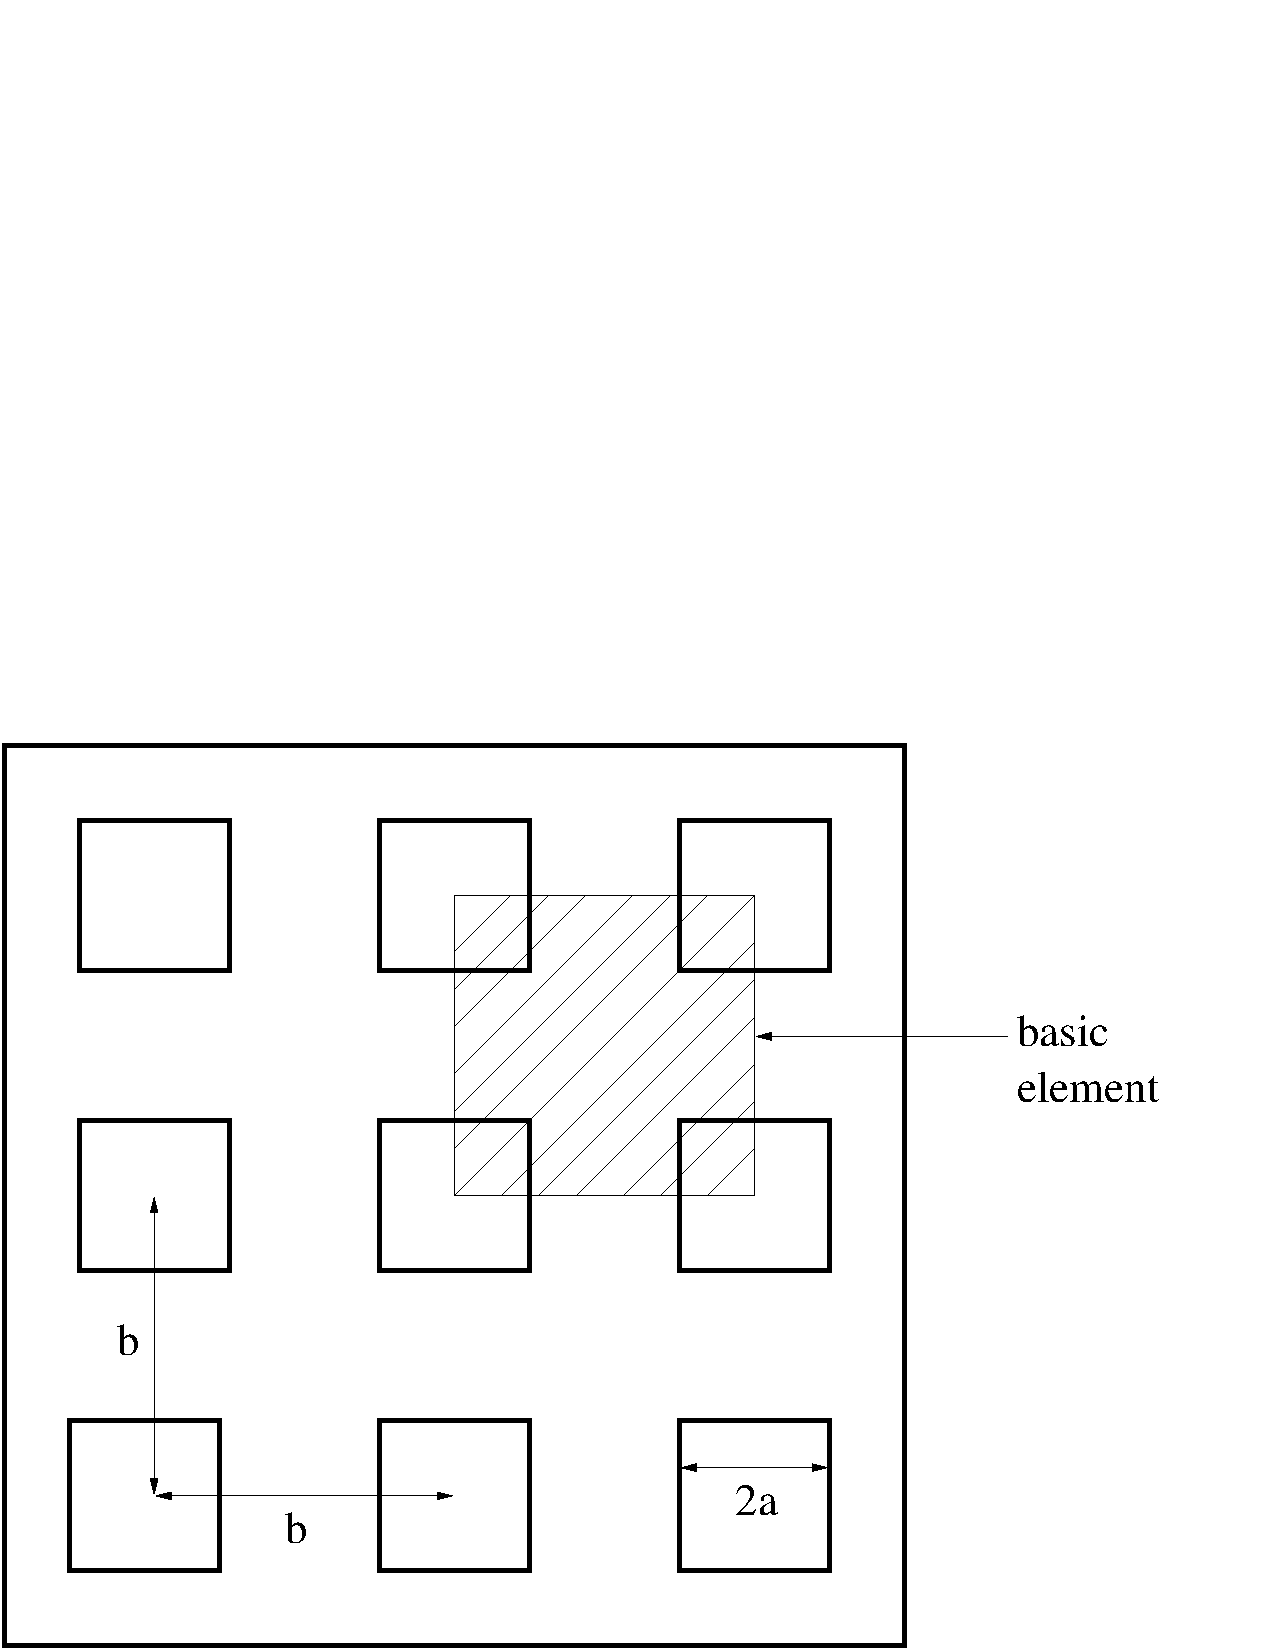
\includegraphics[width=0.6\textwidth]{basic-element}}
\caption{The basic element of the perforated plate consisting of five rectangular
beams}
\label{fg:basic}
\end{figure}

The unit cell of a perforated plate may be assumed to consist of one 
small square plate with side $b-2a$, and of four beams of length $a$ as
shown in Figure~\ref{fg:basic}.
Using approximate formulas an analytical formula for the deformation
energy of the perforated plate is obtained.  
This has to be equal to the deformation energy of 
an unperforated ortoropic membrane. From this condition we get a set of equations
from which the effective parameters may be solved.

The elasticity tensor has three independent components, 
$C_{11}=C_{22}, C_{12}=C_{21}$, and $C_{44}$. 
The expressions for these are
~\cite{pedersen1},
\begin{eqnarray}
C_{11} & = & C_{22} = \frac{E}{b^{2}} \left \{ \frac{b(b-2a)}{1-\nu^{2}} + 
\frac{a(b-2a)^{2}}{b} \right \} \label{eq:C1} \\
C_{12} & = & C_{21} = \frac{\nu E (b-2a)}{b(1- \nu^{2})} \label{eq:C2} \\
C_{44} & = & \frac{E}{4b^{2}(1+ \nu)} \left \{ 2b(b-2a) + \frac{12 K a(b-2a)}{bh^{3}} 
\right\}. \label{eq:C3}
\end{eqnarray} 
where $K$ is a constant\footnote{In article~\cite{pedersen1} there is an error in the definition of
$K$. In the article there is an expression $(b-2a)/h^{3}$, which would make $K$ 
discontinuous at $h=b-2a$.}, 
defined as
\begin{equation}
K= \left \{ \begin{array}{ll}
\frac{1}{3} \left (1-0.63 \frac{b-2a}{h} \right)(b-2a)^{3}h, \quad \mbox{jos  }h>b-2a \\
\frac{1}{3} \left (1-0.63 \frac{h}{b-2a} \right)(b-2a)h^{3}, \quad \mbox{jos  }h<b-2a.  
\end{array}
\right.
\end{equation}

The midplane tension of the perfomarated plate may be reduced to 
lateral stresses of the ortotropic plate by a simple scaling, 
\begin{equation}
 T = \sqrt{(1-4a^{2}/b^{2})} \, T_0 , \label{eq:sigmared}
\end{equation}
where is the tension $T_0$ of the perforated plate. Using this reduced tension and
the modified material parameters of equations~(\ref{eq:C1}),~(\ref{eq:C2}) and~(\ref{eq:C3}) 
the ortoropic plate mimics the behavior of the perforated plate 
when looking at macroscopic quantities. However, the model is not suitable for approximating
maximum stresses around the holes, for example.

\section{Keywords}
\end{versiona}

\sifbegin
\sifitemnt{Solver}{solver id}
\sifbegin
\sifitemnt{Equation}{String SmitcSolver}
\sifitem{Procedure}{File "Smitc"\ "SmitcSolver"}
The procedure which inludes the linear plate model.
\sifitem{Variable}{String Deflection}
This may be of any name as far as it is used consistently also elsewhere.
\sifitem{Variable DOFs}{Integer 3}
Degrees of freedom for the deflection. 
The first degree is the displacment and the two following ones
are its derivatives in the direction of the coordinate axis.
\sifitem{Eigen Analysis}{Logical}
Also the eigenvalues and eigenmodes of the elasticity equation may be computed.
This is done automatically by calling a eigensolver after the original equation has been solved.
The default is \texttt{False}.
\sifitem{Eigen System Values}{Integer}
If the eigenvalues are computed this keyword gives the number of eigenmodes
to be computed. The lowest eigenvalues are always solved for.
\sifitem{Hole Correction}{Logical} 
If the plate is perforated the holes may be taken into account by 
a homogenized model. This is activated with this keyword.
The default is \texttt{False}.
\sifitemnt{Procedure}{File "Smict"\ "SmitcSolver"}
\sifend

\sifitemnt{Material}{mat id}
\sifbegin
\sifitem{Density}{Real}
Density of the plate.
\sifitemnt{Poisson ratio}{Real}
\sifitem{Youngs modulus}{Real}
The elastic parameters are given with Youngs modulus and Poisson ratio.
\sifitem{Thickness}{Real}
Thickness of the plate.
\sifitem{Tension}{Real}
The plate may be pre-stressed.
\sifitemnt{Hole Size}{Real}
\sifitem{Hole Fraction}{Real}
If \texttt{Hole Correction} is \texttt{True} the solver 
tries to find the size and relative fraction of the holes. 
If these are present the hole is assumed to be a square hole.
\sifend

\sifitemnt{Boundary Condition}{bc id}
\sifbegin
\sifitem{Deflection i}{Real}
Dirichlet BC for the components of the deflection, i=1,2,3.
\sifend

\sifitemnt{Body Force}{bf id}
\sifbegin
\sifitem{Pressure}{Real}
Possibility for a body forces. For coupled systems there is a 
possibility to have up to three forces. The two others are then
marked with \texttt{Pressure B} and \texttt{Pressure C}.
\sifitem{Spring}{Real}
The local spring which results to a local force when multiplyed
by the displacement.
\sifitem{Damping}{Real}
The local damping which results to a local force when multiplyed
by the displacement velocity. The spring and damping may also be 
defined as material parameters.
\sifend

\sifend


\begin{versiona}
\bibliography{elmerbib}
\bibliographystyle{plain}
\end{versiona}


%\graphicspath{{./}{aperamp/}}
%\include{aperamp/aperamp}

\graphicspath{{./}{electrostatics1d/}}
\include{electrostatics1d/electrostatics1d}

\graphicspath{{./}{reynolds/}}
\Chapter{Reynolds Equation for Thin Film Flow}

\modinfo{Module name}{\Idx{ReynoldsSolver}}
\modinfo{Module subroutines}{ReynoldsSolver, \Idx{ReynoldsHeatingSolver}}
\begin{versiona}
\modinfo{Module authors}{Peter R�back}
\modinfo{Module status}{Alpha}
\modinfo{Document authors}{Peter R�back}
\modinfo{Document created}{24.10.2007}
\modinfo{Document edited}{24.10.2007}


\section{Introduction}
The flow of fluids is in the continuum level usually described by the Navier-Stokes
equations. For narrow channels this approach is an overkill and usually not even necessary.
Neglecting the inertial forces and assuming fully developed
laminar velocity profiles the flow equations may be reduced in dimension resulting to the 
\Idx{Reynolds equation}.  

The current implementation of the Reynolds equation
is suitable for incompressible and weakly compressible liquids as well as for isothermal and adiabatic ideal gases.
The nonlinear terms for the compressible fluids are accounted for.
The fluid is assumed to be newtonian i.e. there is a direct connection between 
the strain rate and stress. 
The equation may be solved either in steady state or in a transient mode. 

There is an additional solver for postprocessing purposes that computes the 
local heat generation field using the Galerkin method. It also computes the integrals over the
force and heating fields over the whole area.


\section{Theory}

The underlaying assumption of the Reynolds
equation is that the flow in the channel is fully developed and
has thus the Hagen-Poiseuille parabolic velocity profile.
Accounting also for the movement of the planes and leakage trough perforation holes the pressure 
may be solved from the equation
\begin{equation}
\label{eq:reynolds1}
\nabla \cdot \left(\frac{\rho h^{3}}{12\eta}\nabla{p}\right) - Y \rho p = 
\Inv{2} \nabla\cdot \left( \rho h \Vec{v}_t\right) +  h \Der{\rho}{t} + \rho v_n, 
\end{equation}
where $\rho$ is the density, $\eta$ is the viscosity, $p$ is the pressure 
and $h$ is the gap height, $v_t$ is the tangential velocity, and $v_n$ is the velocity in direction of the surface normal~\cite{hamrock04,veijola05b}. 
Holes may be homogenized 
using the flow admittance $Y$ which gives the ratio between pressure drop and mean flow velocity through the 
hole. 

The exact form of the Reynolds equation depends on the material law for density,  $\rho(p)$.
The absolute value of density does not play any role and therefore we may study just the functional forms.
For gases we solve for the pressure variation from the reference pressure $P_0$ rather than for the absolute pressure.
The different functional forms for some idealized material laws are the following:
\begin{eqnarray*}
  \rho \propto & (P_0+p)  \, \, \, \, & \mbox{isothermal ideal gas} \\
  \rho \propto & (P_0+p)^{1/\gamma}  & \mbox{adiabatic ideal gas} \\
  \rho \propto & 1  & \mbox{incompressible} \\    
  \rho \propto & e^{p/\beta}  & \mbox{weakly compressible} .
\end{eqnarray*}
Here $\gamma=C_p/C_V$ is the specific heat ratio and $\beta$ the bulk modulus. 
In discretization of the equations it is also useful to derive the functional dependencies of the 
density derivatives in respect to pressure, 
\begin{eqnarray*}
  \rho_p \propto & 1  \, \, \, \, & \mbox{isothermal ideal gas} \\
  \rho_p \propto & (1/\gamma) (P_0+p)^{1/\gamma-1}  & \mbox{adiabatic ideal gas} \\
  \rho_p \propto & 0  & \mbox{incompressible} \\    
  \rho_p \propto & \rho / \beta  & \mbox{weakly compressible} .
\end{eqnarray*}

In order to improve convergence of the iteration of the nonlinear system some terms including 
differentials of density may be expressed implicitly using pressure. This way equation~(\ref{eq:reynolds1}) 
may be written in the following form:
\begin{equation}
\label{eq:reynolds2}
\nabla \cdot \left(\frac{\rho h^{3}}{12\eta}\nabla{p}\right) - Y \rho p - \rho_p h \Der{p}{t}
- \Inv{2} \rho_p h \Vec{v}_t \cdot \nabla p
= \Inv{2} \rho \nabla \cdot \left( h \Vec{v}_t\right) + \rho v_n.  
\end{equation}


The surface velocity $\Vec{v}$ may also be given in normal cartesian coordinate system. Then the 
normal and tangential components may easily be obtained from
\begin{eqnarray*}
  v_n      & = & \Vec{v}\cdot \Vec{n} \\
  \Vec{v}_t & = & \Vec{v} - v_n \Vec{n} .
\end{eqnarray*}
The normal velocity and gap height are naturally related by
\begin{equation}
  v_n = \Der{h}{t} .
\end{equation}
In transient case the user should make sure that this relationship is honored.

\subsection{Flow admittances of simple geometries}

The flow admittance, $Y$, occurring in the Reynolds equation
may sometimes be solved analytically
for simple hole geometries from the steady-state Stokes equation.
Generally $Y$ depends on the history but here we assume that it is presents the steady-state situation
of the flow~\cite{raback03,veijola05b}.  This means that inertial and compressibility effects are not accounted for. 
%
For cylindrical holes the admittance then yields,
\begin{equation}
  Y = \frac{D^2}{32 \eta b},
\end{equation}
where $D$ is the diameter of the holes and $b$ is the length of the hole.
In case of a narrow slot with width $W$ the admittance is given by
\begin{equation}
  Y = \frac{W^2}{12 b \eta}.
\end{equation}


\subsection{Gas rarefaction effects}

Generally the Reynolds equation could also be used to model nonnewtonian material laws. 
The current implementation is limited to the special case of rarefied gases. 
The goodness of the continuum assumption $\eta$ 
depends on the \Idx{Knudsen number}, $K_n$, which is 
defined by
\begin{equation}
  K_n = \frac{\lambda}{h}, 
\end{equation} 
where $\lambda$ is the mean free path of the molecules and
$h$ is the characteristic scale (here the gap height).
In this solver only the dependence with pressure is taken into account from the formula
\begin{equation}
  \lambda = \frac{1}{1 + p/P_0} \lambda_0 .
\end{equation} 

When the Knudsen number is very small ($K_n \ll 1$)
the gas may be considered as a continuous medium.
When the Knudsen number is in the transition regime
($K_n\approx 1$) we may take the gas rarefaction effect into
account by an effective viscosity.
This accounts for the slip conditions of the flow in the channel by decreasing the viscosity value.
An approximation given by Veijola~\cite{veijola95} is 
\begin{equation}
  \eta = \frac{\eta_0}{1+9.638 K_n^{1.159}}.
\end{equation}
It s relative accuracy is 5 \% in the interval $0 < K_n < 880$.



\subsection{Boundary conditions for the Reynolds equation}

The Reynolds equation may have different boundary conditions.
The natural boundary condition that is obtained by default is 
\begin{equation}
  \Der{p}{n} = 0 .
\end{equation}
This condition may be used at symmetry and closed boundaries. 

If the aspect ratio of the resonator is large then the 
pressure variation at the open sides is small compared to the
values far from boundaries. Then may set Dirichlet boundary conditions ($p=0$) for the
pressure.
However, if the aspect ratio is relatively small
the open side effects should be taken into account. The pressure
variation at the side is not exactly zero while also the open space
has a flow resistance. The pressure derivative at the boundary is approximated
by 
\begin{equation}
  \Der{p}{n} = \frac{p}{L},
\end{equation}
where $L$ is the effective added length of the open sides~\cite{aplac}.
If gas rarefaction is not accounted for then $L=0.8488 h$,
otherwise
\begin{equation}
   L = 0.8488 (1.0 + 2.676  K_n^{0.659}) h.
\end{equation}


\subsection{Postprocessing}

When the equation has been solved the solution may be used to compute some data
for postprocessing purposes. The total force acting on the surface is 
\begin{equation}
  \Vec{F} = \int_A \left ( p \Vec{n} + \frac{\eta}{h} \Vec{v}_t \right) \, dA ,
\end{equation}
where the first term is due to pressure driven flow and the second one due to sliding driven flow.
Also the heating effect may be computed. It consist of two parts: 
pressure driven flow and sliding flow. The local form 
of this is 
\begin{equation}
  \label{eq:heating}
  q = \frac{h^3}{12 \eta} |\nabla p|^2 + \frac{\eta}{h}|\Vec{v}_t|^2 .
\end{equation}
Therefore the total heating power of the system is 
\begin{equation}
  Q = \int_A q \,dA .
\end{equation}
It should be noted that if the velocity field $\Vec{v}$ is 
constant then the integral quantities should fulfill the condition $Q=\Vec{F}\cdot\Vec{v}$.

Note that the above implementation does not take into account the leakege through perforation holes
nor the compressibility effects of the fluids. 



\section{Keywords}

The module includes two different solvers. \texttt{ReynoldsSolver} solves the differential 
equation~(\ref{eq:reynolds2}) while \texttt{ReynoldsHeatingSolver} solves the equation~(\ref{eq:heating}) and
computes the integrals. The second solver only makes sense when the pressure field has already been 
computed with the first one. The second solver uses the same material parameters as the first one. 

\end{versiona}


\subsection*{Keywords for ReynoldsSolver}

\sifbegin
%
\sifitemnt{Solver}{solver id}
\sifbegin
\sifitem{Equation}{String ReynoldsSolver}
A describing name for the solver. This can be changes as long as it is 
used consistanly.
\sifitem{Variable}{String FilmPressure}
The name of the variable may be freely chosen as far as it 
is used consistently also elsewhere. 
\sifitem{Variable DOFs}{Integer 1}
Degrees of freedom for the pressure. This should be 1 which is also the default value.
\sifitem{Procedure}{File "ReynoldsSolver"\ "ReynoldsSolver"}
The name of the module and procedure. These are fixed.
%
\sifitem{Nonlinear System Convergence Tolerance}{Real}
The transient equation is nonlinear if the relative displacement or 
pressure deviation is high. The iteration is continued till 
the relative change in the norm falls under the value given by this keyword.
\sifitem{Nonlinear System Max Iterations}{Integer}
This parameter gives the maximum number of nonlinear iterations required in the solution.
This may be set higher than the typical number of iterations required as the 
iteration procedure should rather be controlled by the convergence tolerance.
%

\sifend

\sifitemnt{Material}{mat id}
\sifbegin
\sifitem{Gap Height}{Real}
Height of the gap where the fluid is trapped. If the case is transient the user should herself 
make sure that also this variable has the correct dependence on time. 
\sifitem{Surface Velocity i}{Real}
The velocity of the moving body may be given in either cartesian coordinates, or in ones that 
are already separated to normal and tangential directions. In the first case the velocity components 
are given with this keyword with \texttt{i=1,2,3}.
\sifitem{Tangent Velocity i}{Real}
For setting the tangential velocity (i.e. sliding velocity) use this keyword with 
\texttt{i=1,2,3}.
\sifitem{Normal Velocity}{Real}
Normal velocity is the velocity in the direction of the surface normal. Typically a negative value
means contraction. 
%
\sifitem{Viscosity}{Real}
Viscosity of the gas.
%
\sifitem{Viscosity Model}{String} 
The choices are \texttt{newtonian} and \texttt{rarefied}. The first one is also the default.
%
\sifitem{Compressibility Model}{String} 
The choices are \texttt{incompressible}, \texttt{weakly compressible},
\texttt{isothermal ideal gas}, and \texttt{adiabatic ideal gas}.
%
\sifitem{Reference Pressure}{Real}
Reference pressure is required only for the ideal gas laws. 
%
\sifitem{Specific Heat Ratio}{Real}
This parameter is only required for adiabatic processes. For ideal
monoatomic gases the ratio is $5/3$. Only required for the adiabatic compressibility model.
%
\sifitem{Bulk Modulus}{Real}
The parameter $\beta$ in the weakly compressible material model. 
%
\sifitem{Mean Free Path}{Real}
If the viscosity model assumes rarefied gases the mean free path of the gas molecules 
in the reference pressure must be given.
%
\sifitem{Flow Admittance}{Real}
The steady-state flow admittance resulting from perforation, for example.
%  
\sifend	
%
\sifitemnt{Boundary Condition}{bc id}
\sifbegin
\sifitem{FilmPressure}{Real}
Sets the boundary conditions for the pressure.
Usually the deviation from reference pressure is zero at the boundaries.
%
\sifitem{Open Side}{Logical}
The open end effect may be taken into account 
by setting this keyword \texttt{True}.
\sifend
\sifend


\subsection*{Keywords for ReynoldsHeatingSolver}

This solver uses largely the same keywords that are already defined above. Only the Solver
section has its own keyword settings. This solvers should be active in the same bodies than the 
\texttt{ReynoldsSolver}. 

\sifbegin
%
\sifitemnt{Solver}{solver id}
\sifbegin
\sifitem{Equation}{String ReynoldsHeatingSolver}
A describing name for the solver. This can be changes as long as it is 
used consistently.
\sifitem{Variable}{String FilmHeating}
The name of the variable may be freely chosen as far as it 
is used consistently also elsewhere. 
\sifitem{Variable DOFs}{Integer 1}
Degrees of freedom for the pressure. This should be 1 which is also the default value.
\sifitem{Procedure}{File "ReynoldsSolver"\ "ReynoldsHeatingSolver"}
The name of the module and procedure. These are fixed.
%
\sifitem{Reynolds Pressure Variable Name}{String}
The name of the field that is assumed to provide the pressure field. The default is \texttt{FilmPressure}.
\sifend
\sifend


\bibliography{elmerbib}
\bibliographystyle{plain}


%\graphicspath{{./}{aplacinterface/}}
%\include{aplacinterface/aplacinterface}

\graphicspath{{./}{phasechange/}}
\chapter{Phase Change}

\modinfo{Module name}{\Idx{PhaseChangeSolve}}
\modinfo{Module subroutines}{PhaseChangeSolve}
\modinfo{Module authors}{Peter R�back, Jussi Heikonen, Juha Ruokolainen}
\modinfo{Document authors}{Peter R�back}
\modinfo{Document created}{22.10.2004}
\modinfo{Document edited}{28.4.2006}


\section{Introduction}


The boundary which separates a liquid and solid phase of a material is called 
a phase change or \Idx{Stefan boundary}. 
This subroutine defines the position of the phase change boundary.
The phase change problem may occur for example in crystal growth and 
casting processes. 

Phase change problems may be modeled using a fixed grid or alternatively distorting the grid
so that the phase change boundary surface is exactly described by the computational mesh. 
Elmer has an internal fixed grid phase change model where the phase change is modelled
by modifying the definition of heat capacity.
This method is not limited by topological constraints but its accuracy 
may be questionable. If the 
phase change occurs within very sharp temperature interval
the current method where the phase change surface is set exactly 
should be preferred,

The current methodology is limited into two dimensional cases
where the phase change surface is nearly aligned with either of the 
coordinate axis.


\section{Theory}

The phase change from solid to liquid occurs at the 
\Idx{melting point} $T_m$. At the boundary the temperatures of the 
liquid and solid are therefore equal to that. 
The phase change results to a change in the internal energy
known as the latent heat $L$. 

The \Idx{latent heat} makes the diffusive heat flux over the boundary discontinuous 
and results to the so called Stefan condition
\begin{equation} 
\label{e:stefan}
L\rho \Vec{v}  \cdot \Vec{n} =
(\kappa_{s}\nabla T_{s}-\kappa_{l}\nabla T_{l})\cdot \Vec{n},
\end{equation}
where $\Vec{n}$ is the normal of the phase change boundary, 
$\Vec{v}$ is the velocity of the phase change boundary,
$\rho$ is the density of the solid 
and $T_{s}$ and $T_{l}$ are the temperatures of the solid and liquid phases,
and $\kappa_{s}$ and $\kappa_{l}$ are the thermal 
conductivities, respectively.
In steady state the velocity of the phase change boundary should be equal to pull velocity,
$\Vec{v}=\Vec{V}$ (bulk velocity of the solid phase).


\subsection{Steady state algorithm} 

In steady state case the basic algorithm is based mainly on geometrical ideas.
First the heat equation for temperature $T$ is solved by using a flux 
condition for the interface
\begin{equation}
  q =  L \rho V_n . 
\end{equation}
Thereafter the next approximation for the 
phase change surface may be found by going trough each element and 
creating a list of line segments $E_j$ on the isosurface.
This is basically the zero level-set of the field $T-T_m$.
Each line segment is defined by two coordinate $\Vec{x}_{j,1}$ and $\Vec{x}_{j,2}$.
The surface is then updated by mapping the current phase change surface to the 
line segments. For the moment a $N^2$ algorithm is used for the mapping. For larger
cases a more robust search algorithm might be implemented. 

For example, if a free surface is almost aligned along the x-axis,
then for a node $(x_i,y_i)$ on the boundary the 
proposed change of the point $i$ in the 
y-direction is 
\begin{equation}
  s_y = (y_{j,1} - y_i) +  ( x_i - x_{j,1}) \frac{y_{j,2}-y_{i,1}}{x_{j,2}-x_{j,1}}
\end{equation}
assuming that $x_i \in [x_{j,1},x_{j,2}]$ while $s_x = 0$.


In many cases the simple geometrical search algorithm converges
very slowly. The reason is the explicit character of the algorithm that fails to account
for the change in the temperature field caused by the moving phase change boundary.
This limitation may be partially overcome using suitable under- or over-relaxation. 
This relaxation parameter may also be tuned during the iteration using lumped 
quantities such as the proposed change in the volume of the phases
that may be expressed as
\begin{equation}
  U = \int_A \Vec{s} \cdot \Vec{n} \, dA . 
\end{equation}
The proposed volume changes form a series, $U^{(0)}, U^{(1)}, \ldots, U^{(m-1)}, U^{(m)}$.
Assuming that the series is a geometric one we may estimate the required relaxation
factor that would give the correct phase change boundary at just one iteration,
\begin{equation}
  c^{(m)} = c^{(m-1)} \frac{U^{(m-1)}}{U^{(m-1)}-U^{(m)}}.
\end{equation} 
In numerical tests this formula was found occasionally to overshoot and 
therefore a less aggressive version is used instead,
\begin{equation}
  c^{(m)} = c^{(m-1)} \frac{1}{2}\frac{U^{(m-1)}+U^{(m)}}{U^{(m-1)}-U^{(m)}}.
\end{equation} 
The use of the lumped model requires that the temperature field is described accurately enough.
To ensure numerical stability the factor $c$ should have a upper and lower limits.
After the factor has been defined the suggested displacements are simply scaled with it,
$\Vec{s}' = c \Vec{s}$.

It is also possible to accelerate the solution locally using a Newton kind of iteration.
If the basic algorithm has already been applied at least twice we may estimate the sensitivity of the 
local temperature to the moving interface and using this information to estimate a new change,
\begin{equation}
  s^{(m)} =   \frac{T_m - T^{(m)}}{T^{(m)} - T^{(m-1)}} s^{(m-1)} .
\end{equation}
This algorithm might be a better option if the 
phase change surface is such that there is not much correlation between the displacements at the
extreme ends. However, the algorithm may be singular if the isotherms of consecutive iterations
cross. Any point $i$ where $T^{(m-1)}_i \approx T^{(m)}$ leads to problems that
may be difficult to manage. This handicap may rarely limit the usability of the otherwise robust and
effective scheme.


\subsection{Transient algorithm}

In transient case the interface is set to be at the melting point when 
solving the heat equation. From the solution a heat flux is then obtained from
\begin{equation}
\Vec{q} = \kappa_{s}\nabla T_{s}-\kappa_{l}\nabla T_{l}.
\end{equation}
Now this heat flux is assumed to be used for the melting of the 
solid phase into liquid phase. 
Assuming again that the phase change boundary is mapped to the new position
moving it only in the $y$-direction we get 
from equation~(\ref{e:stefan}) the velocity in the $y$-direction,
\begin{equation}
  \rho L n_y ( v_y - D_v \nabla^2 v_y) 
= \Vec{q} \cdot \Vec{n}.
\end{equation}
Here an artificial diffusion $D_v$ has been added since the algorithm otherwise 
is prone to numerical oscillations. In order for the diffusion not to affect the results significantly 
it must fulfil the condition $D_v << h^2$ where $h$ is the size of the 1D elements. 

The corresponding displacement is easily obtained from multiplication
$u_y = v_y \, dt$, where $dt$  is the timestep.
However, in the current formulation this is also done using the 
Galerkin method since the possibility of an additional diffusion factor
is included. Therefore the equation is of the form,
\begin{equation}
  \Der{u_y}{t} - D_u \nabla^2 u_y = v_y.
\end{equation}

In continuous processes the triple point may be used to define the 
pull velocity so that at the point the solution of the equation vanishes.
In case the pull occurs in the $y$-direction this 
means that $V_y = v_y$.

The transient algorithm is ideally suited for relatively small time-steps
where the change in the position is small compared to the other dimensions of the problem.
Otherwise the transient algorithm may result to spurious oscillations.
However, often the timestep size is most severely limited by the flow computations. 
Therefore it may be possible to boost the convergence towards the true operation
regime by multiplying the suggested change by a constant factor. 



\subsection{Hybrid algorithm}

The transient and steady-state algorithm are difficult to apply to cases 
with many different time-scales. The steady-state algorithm converges rapidly to the 
desired shape, however it does not have the inertia that would resist temporal 
fluctuations. The transient algorithm, on the other hand, requires too many iterations 
to be feasible. For that aim we study hybrid algorithms that would combine some of the 
best properties of both methods.

The desired form of the hybrid algorithm would be based on a  
\Idx{Robin boundary condition} for the temperature. 
\begin{equation}
  q_n = L\rho V_n + g (T - T_m).
\end{equation}
This reduces to a Dirichlet condition when $g \rightarrow \infty$ and
to the flux condition when $g=0$. On the other hand the Stefan condition
may be expressed as 
\begin{equation}
  q_n = L\rho ( V_n - v_n ),  
\end{equation}
We use the following approximations
\begin{equation}
  v_n \approx \frac{dn}{dt} \approx \frac{1}{dt} \frac{1}{\Der{T}{n}} ( T - T_m ) .
\end{equation}
The normal derivative of temperature may be approximated by 
\begin{equation}
  \Der{T}{n} = \frac{\kappa\Der{T}{n}}{\kappa} \approx \frac{L \rho V_n }{p \kappa}
\end{equation}
where $p$ is the fraction of the heat flux that goes into solidification. 
Combining the above yields,
\begin{equation}
  q_n = L \rho V_n + g (T_m - T)
\end{equation}
where 
\begin{equation}
  g = \frac{p \kappa}{dt \, V_n} 
\end{equation}
which is an equation of the desired form.
For $dt \rightarrow \infty$ this
retains the original steady state algorithm while for shorter timesteps the 
inertia of the interface is naturally produced. 

After the heat equation with the Robin condition has been solved there
is possible two ways of tuning the interface positions. The first one would use
the geometric ideas of the steady state algorithm. However, the instantaneous 
temperature field may be such that there is no well defined temperature 
isoline that would define the interface position. Therefore
we rather use the transient algorithm to update the position. 
After the solution the disbalance in the heat flux may be computed from 
\begin{equation}
  dq_n = g (T_m - T)
\end{equation}
and the interface velocity from
\begin{equation}
  v_n = \frac{g}{L \rho} (T - T_m).
\end{equation}
Once the normal velocity $v_n$ is computed one may proceed as in the 
transient case. 

The nice property of the hybrid algorithm is that the proposed interface velocity
should not be sensitive on the coefficient of the Robin boundary condition. 
This way the coefficient may be partly chosen so that the convergence 
is optimal. 



\section{Applicable cases and limitations}

The method has some limitations which are described below
\begin{itemize}
\item Limited to 2D and axisymmetric cases.
\item Phase change surface must be nearly aligned with either of the main axis. 
To be more precise the boundary must in all instances be such that for each coordinate there
is only one point on the boundary.   
\item Melting point is assumed to be constant 
\item It should be noted that the solver only gives the position of the phase change 
boundary. In order to modify the whole geometry a mesh update solver must 
be applied. 
\end{itemize}


\section{Keywords}

\sifbegin
\sifitemnt{Solver}{solver id}
\sifbegin
\sifitemnt{Equation}{String "Phase Change"}
\sifitem{Procedure}{File "PhaseChangeSolve"\ "PhaseChangeSolve"}
The subroutine that performs the phase change analysis.
%
\sifitem{Variable}{String PhaseSurface}
The variable for the PhaseSurface coordinate.
This may be of any name as far as it is used consistently also elsewhere.
\sifitem{Variable DOFs}{Integer 1}
Degrees of freedom for the free surface coordinate, the default.
%
\sifitem{Phase Change Variable}{String}
By default the phase change analysis uses \texttt{Temperature} as the 
active variable. The analysis may be performed also to any other scalar
variable given by this keyword
%
\sifitem{Nonlinear System Relaxation Factor}{Real}
Giving this keyword triggers the use
of  relaxation in the phase change solver.
Using a factor below unity may sometimes be required to achieve convergence.
Relaxed phase change variable is defined as follows:
$$
 u^{'}_i = u_i + \lambda s_{i-1},
$$
where $\lambda$ is the factor given with this keyword. The default value for the relaxation factor
is unity. If using the lumped model to accelerate the solution the final relaxation factor will the product of 
the two.
%
\sifitem{Long Transition Timestep}{Real}
There are three different regimes that may be used. This one
defines the timestep at which the steady algorithm changes to 
medium timestep algorithm.
%
\sifitem{Short Transition Timestep}{Real}
This keyword
defines the timestep at which the medium timestep algorithm is switched to
short timestep algorithm. 
%
\sifitem{Medium Timestep Algorithm}{String}
The medium timestep algorithm. The options are ``steady'', ``hybrid'', and ``transient''.
\sifitem{Short Timestep Algorithm}{String}
The same options as the previous keyword.
\sifend
%
Some variables have a function only in steady state while others 
relate to the transient case. Below are the 
steady-state parameters for the  \texttt{Solver} section.
%
\sifbegin
\sifitem{Nonlinear System Newton After Iterations}{Integer}
The local Newton type of iteration may be set active after 
a number of iterations given by this keyword.
%
\sifitem{Nonlinear System Newton After Tolerance}{Real}
The Newton type of iteration may also be activated after a sufficiently small change in the norm.
This keyword gives the limit after which Newton iteration is triggered on. 
%
\sifitem{Lumped Newton After Iterations}{Logical}
The phase change solver may be accelerated pointwise, or by using a lumped model to determine
an optimal relaxation factor for the whole solution. This keyword activates the lumped model
procedure. 
%
\sifitem{Lumped Newton Limit}{Real}
The lumped approach sometimes gives too high or too small relaxation factors. 
This may happen particularly at the very vicinity of the solution where the 
approximation errors have a greater effect. 
%
\sifitem{Triple Point Fixed}{Logical}
This keyword enforces the triple point to be fixed. Depending on the type of algorithm this
may mean different things. For the steady algorithm this means that the temperature used for
finding the isotherm is set to be the temperature of the triple point. Hence the 
isoterm will travel through the triple point. In the transient algorithm this means that 
the interface velocity is tuned so that the velocity at the triple point is zero.
%
\sifitem{Use Absolute Norm for Convergence}{Logical}
The steady-state solver returns the maximum phase change update as the 
norm and therefore this
flag should be set \texttt{True}.
The transient solver gives the norm of the finite element solution in the
usual manner. 
\sifend
%
The following keywords may be defined in the transient algorithm.
\sifbegin
\sifitem{Pull Rate Control}{Logical}
In transiet case the pull rate may be set so that the triple point remains at a fixed 
position. The feature is activated setting this keyword \texttt{True}.
%
\sifitem{Velocity Relaxation Factor}{Real}
The relaxation factor for the crysrallization velocity field. 
%
\sifitem{Velocity Smoothing Factor}{Real}
The velocity diffusion factor of the interface, $D_v$.
%
\sifitem{Transient Speedup}{Real}
The factor at which the change in the boundary position is changed in the transient 
case. This may be used to speedup the transient convergence. 
%
\sifitem{Nonlinear System Max Iterations}{Integer}
In case the pull-rate control is used the phase change algorithm may have
to be solved several times in order to define the consistent pull-rate. 
This keyword gives the maximum number of iterations.
The steady state algorithm is solved by just one sweep.
%
\sifitem{Nonlinear System Convergence Tolerance}{Real}
The tolerance for terminating the transient algorithm.
\sifitem{Stabilize}{Logical}
The transient algorithm may require stabilization 
which decreases the oscillations of the solution. 
%
\sifend
%
\sifitemnt{Body}{body id}
\sifbegin
\sifitemnt{Solid}{Logical}
\sifitem{Liquid}{Logical}
The solver requires information on which of the materials in the system is solid
and which is liquid. Currently the solver assumes that both the liquid and 
solid is uniquely defined. 
\sifend

\sifitemnt{Material}{mat id}
\sifbegin
\sifitem{Melting Point}{Real}
The melting point is the temperature at which the transition form solid to liquid occurs.
The melting point is assumed to be constant.
\sifitem{Heat Conductivity}{Real}
In a transient case the heat conductivities of the both materials must be given.
\sifitem{Density}{Real}
Density may be needed in the computation of the surface normals. 
By default, the normals point out from the denser of the two materials.
\sifitem{Pull Velocity i}{Real}
For the transient algorithm the pull velocity of the boundary may be given
with this keyword. 
%
\sifitem{Latent Heat}{Real}
The latent heat is the specific internal energy related to the phase change.
The latent heat may also be a variable. 
\sifend
%
\sifitemnt{Boundary Condition}{bc id}
\sifbegin
\sifitem{Body Id}{Integer}
The phase change solver operates usually on a boundary of a two-dimensional 
domain. Technically the equation on the boundary is treated in a normal finite element
manner and therefore the boundary must be defined to be the body where the 
equation is to be solved. Usually this would be the next free integer in the
list of bodies. 
\sifend
The module also includes subroutines \texttt{PullRate} and \texttt{PullPosition}
that may be used to give
boundary conditions for the mesh update solver.
These subroutines relate to transient case. 
The syntax of the subroutines is as the following,
%\sifbegin
\ttbegin
Mesh Update 2 = Variable Coordinate 1
  Real Procedure "PhaseChangeSolve" "PullPosition"
\ttend
and 
\ttbegin
Convection Velocity 2 = Variable Coordinate 1
  Real Procedure "PhaseChangeSolve" "PullRate"
\ttend
%\sifend
For the steady state case the heat equation often requires the 
heat flux as a boundary condition. For this there is also a precompiled 
subroutine that may be activated by the following lines in the command file,
%\sifbegin
\ttbegin
Heat Flux BC = Logical True
Heat Flux = Variable Coordinate 1
  Real Procedure "PhaseChangeSolver" "MeltingHeat"
\ttend
%\sifend
\sifend





\bibliography{elmerbib}
\bibliographystyle{plain}



\graphicspath{{./}{freesurface2d/}}
\Chapter{Free Surface with Constant Flux}

\modinfo{Module name}{\Idx{FreeSurfaceReduced}}
\modinfo{Module subroutines}{FreeSurfaceReduced}
\begin{versiona}
\modinfo{Module authors}{Peter R�back}
\modinfo{Document authors}{Peter R�back}
\modinfo{Document edited}{August 5th 2002}


\section{Introduction}

The determination of free surface is often an essential part of solving
a fluid dynamics problem. Usually the surface is found by solving a 
free surface equation resulting from force balance, 
or by finding the free surface from zero flux condition.
In some extreme cases both of these methods were found to fail and 
therefore an alternative approach was taken. The method can 
only be applied to stationary 2D or axisymmetric flows where the total flux 
is conserved. This is the case, for example, in many \Idx{coating} and 
\Idx{drawing} processes.


\section{Theory}

\index{mass conservation}
The determination of the free surface takes use of the 
conservation of mass. If the flow is stationary the mass flux through all 
planes cutting the flow must be same.
In the following we concentrate on the axisymmetric case which has more 
applications than the 2D case. 

In the axisymmetric case the mass flux is obtained from 
\begin{equation}
  f(R,z) = \int_{R_0}^{R} (\vec{u}\cdot\vec{n}) \, r ds.
\end{equation}
The free surface is set by finding 
a surface profile $R(z)$ such that the integral is
constant for all nodes on the surface, or 
\begin{equation}
  f(R,z_j) = f(R_1,z_1) \ \ \ \ \forall j \in  [1,M].
\end{equation}
Note that the factor $2\pi$
has been consistently omitted since it has no bearing
to the shape of the free surface.

The subroutine uses simple heuristics to determine the direction 
of the flow on the free surface. The first upwind node $z_1$ on the free surface is 
assumed to be fixed and the corresponding flux is $f_1$.
The new radius is set approximately by assuming that the 
added or removed flow has the same velocity as the 
velocity on the surface.
Then the corrected radius is found from
\begin{equation}
  u_n R^{(m)} \, d R^{m} = f(R^{(m)},z) - f(R_1,z_1)
\end{equation}
or
\begin{equation}
  R^{(m+1)} = R^{(m)} + \frac{f(R^{(m)},z) - f(R_1,z_1)}{u_n R^{(m)}}.
\end{equation}
After the new profile is being found the 
element nodes are moved to the new positions.
The nodes that are not on the surface may be mapped in 
many different ways. The straight-forward strategy is to use linear 1D mapping.
Also more generic 2D mapping may be used.
 
The free surface and the fluid flow must 
be consistent and therefore the system must 
be solved iteratively.
When convergence of the coupled system has been obtained 
the suggested $d R$ vanishes and the free surface solver 
does not affect the solution.

Sometimes the free surface solver overshoots and therefore it may
be necessary to use relaxation to suppress the large 
changes of the solution.

Note that the free surface solver is simple based on mass conservation. No
forces are applied on the free surface. If surface tension needs to be taken 
into account it may be done while solving the Navier-Stoke equation.


\section{Applicable cases and limitations}

The method has some limitations which are inherent of the method:
\begin{itemize}
\item Limited to steady-state simulations.
\item Limited to 2D and axisymmetric cases.
\item If there is back-flow within the free surface flow the correctness of the 
solution is not guaranteed.
\end{itemize}
Some limitations result from the current implementation:
\begin{itemize}
\item The free surface must be oriented so that the flow is on its negative side.
\item There may be several free surfaces of this type but they must be directed
	the same way.
\item The line integral from $R_0$ to $R$ may cause some difficulties in 
	unstructured meshes. Therefore structured meshes are favored.
\item At the moment density is assumed to be constant and
 	therefore only incompressible fluids may be considered.
\end{itemize}



\section{Keywords}
\end{versiona}

\sifbegin
\sifitemnt{Solver}{solver id}
\sifbegin
\sifitemnt{Equation}{String "Free Surface Reduced"}
\sifitem{Variable}{String dx}
The change in the free surface coordinate.
This may be of any name as far as it is used consistently also elsewhere.
\sifitem{Variable DOFs}{Integer 1}
Degrees of freedom for the free surface coordinate.
\sifitem{Procedure}{File "FreeSurfaceReduced"\ "FreeSurfaceReduced"}
The following four keywords are used for output control.
\sifitem{Perform Mapping}{Logical}
If this keyword is {\tt True} the coordinate 
mapping is done locally by using linear 1D mapping.
This is also the default. 
Also 2D mapping is possible by using a separate 
mesh update solver. Then the keyword should be set to \texttt{False}.
\sifitem{Nonlinear System Relaxation Factor}{Real}
The changes in the free surface may be relaxed. The 
default is no relaxation or value 1.0

\sifitem{Nonlinear System Convergence Tolerance}{Real} 
This keyword gives a criterion to
terminate the nonlinear iteration after the maximum change in the 
free surface coordinate is small enough
\begin{equation}
 \max || d R / ( R - R_0 ) ||  < \epsilon  \nonumber
\end{equation}
where $\epsilon$ is the value given with this keyword.
\sifend

\sifitemnt{Boundary Condition}{bc id}
\sifbegin
\sifitem{Free Surface Reduced}{Logical}
Must be set to {\tt True} for the free surface when the solver is used.
The boundary must be simply continuous.
\sifitem{Free Surface Number}{Integer}
If more than one free surface of the reduced type is present simultaneously
they must somehow be separated. This keyword is for that purpose.
The surfaces should be ordered from 1 to the number or free surfaces.
Value 1 is also the default if the surface is active.
Note that free surfaces with different numbers should be aligned the same way and should 
not touch each other.
\sifitem{Free Surface Bottom}{Logical}
If this flag is free it sets the lower boundaries of integration 
when solving for the free surface. Note that this surface should not touch any of the 
free surfaces. A free surface is automatically a lower boundary for another 
free surface.
\sifend
If mapping is not performed within the solver also boundary conditions
for the mapping are required. Surface tension may be taken into account 
while solving the Navier-Stokes equation. The proper keywords for 
activating the surface tension are explained in the manual of the Navier-Stokes solver.
\sifend



%\bibliography{elmerbib}
%\bibliographystyle{plain}




% Utility solvers - No new physics

\graphicspath{{./}{rigidbody/}}
\Chapter{System Reduction for Displacement Solvers}

\modinfo{Module name}{\Idx{RigidBodyReduction}}
\modinfo{Module subroutines}{RigidBody}

\begin{versiona}
\modinfo{Module authors}{Antti Pursula}
\modinfo{Document authors}{Antti Pursula}
\modinfo{Document edited}{August 27th 2003}


\section{Introduction}

\index{reduced order model} This module is used to reduce and simplify
the computation of a displacement solver when the problem includes
rigid blocks. In such a case, it is often difficult for iterative
solvers to find a solution for the full system, and direct solvers
become obsolite when the system is large enough. The convergence and
also the speed of the solution can be substantially improved when the
degrees of freedom corresponding to the nodes belonging in the rigid
blocks are reduced onto the 6~DOFs (3~in~2D) of the corresponding
rigid body. In the module, the reduction is achieved via a
\Idx{projection matrix}.

Additionally, the routine automatically eliminates the degrees of
freedom corresponding to the Dirichlet boundary conditions. It is also
possible to request the elastic regions to be extended into the rigid
blocks. There is also possibility to reorder the reduced matrix
elements to decrease its bandwidth. 


\section{Theory}

The module starts with normally constructed matrix equation for the
unknown displacements $x$, $Ax=b$. Let us assume that the nodes are
ordered in such a way that the first $n$ elements of the vectors
correspond to the elastic parts of the structure and the remaining $m$
elements correspond to the rigid parts of the structure. The goal is
to reduce the $(n+m)\times (n+m)$ matrix $A$ to a $(n+\alpha k)\times
(n+\alpha k)$ matrix $B$, where $k$ is~3 for 2D and~6 for 3D problems
and $\alpha$ is the number of rigid blocks present. Reductions are
made also for the vectors so that finally the matrix equation reads
$Bu = f$.

The relation between the unknowns is 
\begin{equation}
x = Pu,
\end{equation}
where the projection matrix $P$ ties the nodes in the rigid bodies to
the same displacements in coordinate directions and the same rotations
about the coordinate axis. The rotations are defined with a coordinate
system whose origin is at the center of each rigid body.  For the right
hand sides we can write
\begin{equation}
f = Qb,
\end{equation}
where the matrix $Q$ sums the forces and torques present at the nodes
in rigid bodies for a resultant force and torque of the center point
of the corresponding rigid body. In both mappings, the rotations are
linearized so the module is valid only for cases where the rotations
are small.

Using these definitions, we have
\begin{equation}
Ax=APu=b
\end{equation}
and
\begin{equation}
Bu=f=Qb.
\end{equation}
Combining the equations gives $Bu=QAPu$ and thus
\begin{equation}
B = QAP.
\end{equation}
With a suitable order of the rotations one can write 
\begin{equation}
Q=P^T \equiv C,
\end{equation}
and
\begin{equation}
B = CAC^T.
\end{equation}
The matrix $C$ has a identity matrix block of size $n\times n$ which
keeps the elastic nodes intact, and a projection block of size
$\alpha k\times m$. 

The reduced order solution $u$ is transformed back to the original
nodes by the same mapping
\begin{equation}
x=C^T u.
\end{equation}


\section{Applicable cases and limitations}

The module works for
\begin{itemize}
\item Linear steady-state problems
\item Linear transient problems
\item Eigen analysis
\item Quadratic eigenproblems
\end{itemize}
%
There are following limitations:
\begin{itemize}
\item Rigid blocks should not have common nodes (there should be
elastic nodes in between rigid blocks)
\item If a Dirichlet bc is given on a node of a rigid block then the
entire rigid block is assumed to be fixed in all directions
\end{itemize}



\section{Keywords}
\end{versiona}

\sifbegin
\sifitemnt{Body}{body id}
\sifbegin
  \sifitem{Rigid Body}{Logical}
Value {\tt True} defines the rigid body.
\sifend
\sifitem{Solver}{solver id}
The module does not need a separate solver but
a call in the stress analysis,
or the elasticity solver in the linear mode. 
\sifbegin
\sifitemnt{Equation}{String Stress Analysis}
\sifitemnt{Variable}{String Displacement}
\sifitem{Variable DOFs}{Integer}
It is important to give the DOFs right, either 2 or 3 depending on
the dimension.
\sifitem{Before Linsolve}{File "RigidBodyReduction"\ "RigidBody"}
The model order reduction is performed after the matrix has been assembled
but before the matrix equation has been solver. The matrix equation is 
modified to a smaller equation and the new equation is solved within the subroutine.
\sifitem{Eigen Analysis}{Logical}
It is possible to use the model order reduction with modal analysis, as
well as with static and transient cases.
\sifitem{Eigen System Values}{Integer}
The number of eigen values to be computed.
\sifitemnt{Eigen System Damped}{Logical}
\sifitem{Eigen System Use Identity}{Logical [True]}
The reduction is possible also with quadratic (damped) eigenproblems.
\sifitem{Optimize Matrix Structure}{Logical}
If true, the matrix structure is optimized. This feature is recommended 
since the reduced matrix has often very scattered structure. The
optimization is performed with the Cutholl-McKee algorithm.
\sifitem{Reverse Ordering}{Logical}
This flag can be used to reverse the matrix ordering if the matrix
structure is optimized, resulting in reverse Cuthill-McKee ordering.
\sifitem{Extend Elastic Region}{Logical}
If true, the elastic regions of the geometry are extended into the rigid 
block. This feature allows taking into account the bending in the joints 
between elastic and rigid parts.
\sifitem{Extend Elastic Layers}{Integer}
Defines the number of element layers that the elastic regions are extended.
\sifitem{Output Node Types}{Logical}
Writes in the ElmerPost output file a variable describing the status of 
each node in the geometry. The variable has value 0 for elastic nodes,
-1 for rigid blocks that are fixed due to a Dirichlet boundary condition,
and a positive integer for separate rigid blocks. The variable may be 
used to check that the reduction is performed on the right blocks, and to
check how many layers the elastic regions should be extended, for example.
\sifitem{Additional Info}{Logical}
If true, additional information is written about the performed tasks
during the simulation. 
\sifend
\sifend


\begin{versiona}
\section{Examples}

\begin{figure}[tbhp]
  \vspace{-25mm}
  \centerline{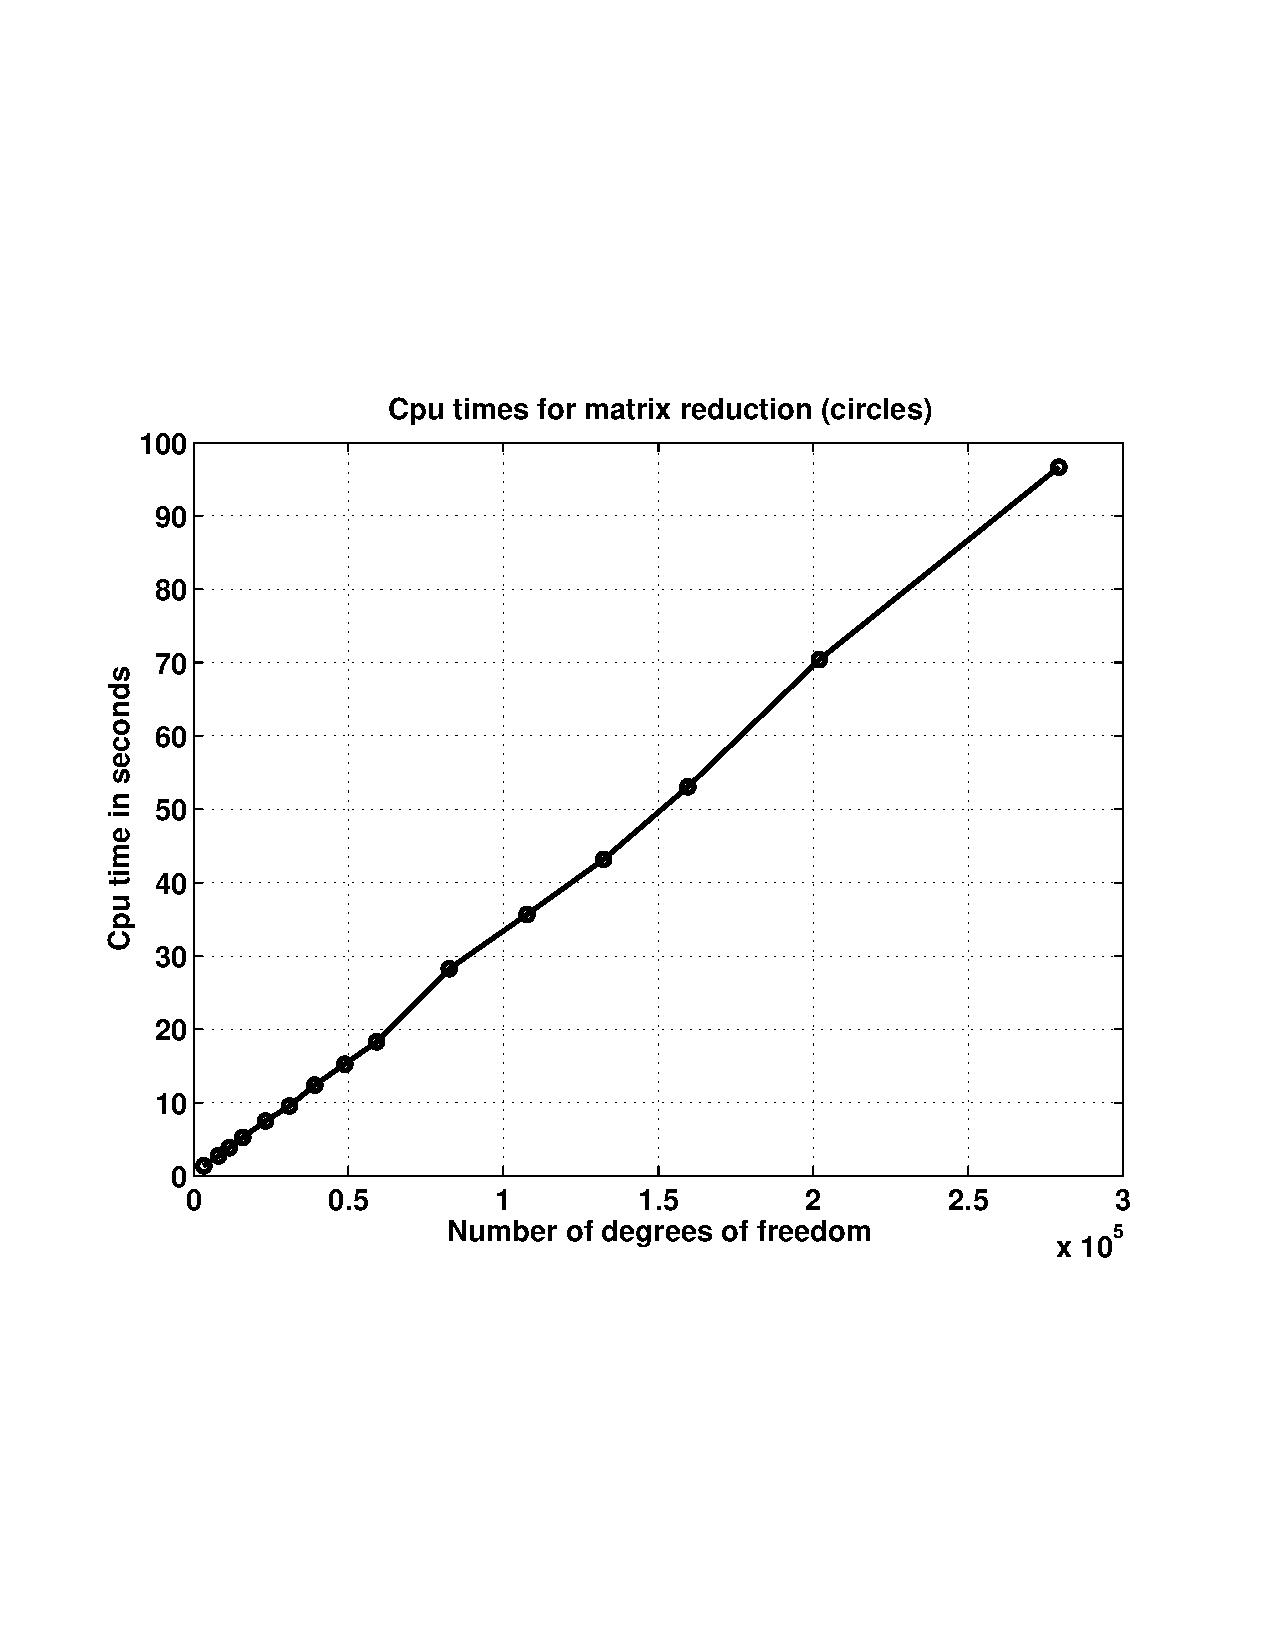
\includegraphics[width=0.6\textwidth]{reduction_cpu.pdf}}
  \vspace{-25mm}
  \caption{The cpu time required for the matrix reduction operations
  depends linearly on the degrees of freedom in the system.}
\end{figure}

%\begin{figure}[tbhp]
%  \centerline{\includegraphics[width=0.5\textwidth]{modes.ps}}
%  \caption{Two eigenmodes (1st and 5th) of a supported structure
%  calculated using matrix reduction.}
%\end{figure}

\end{versiona}


\graphicspath{{./}{artifcomp/}}
\chapter{Artificial compressibility for FSI}

\modinfo{Module name}{\Idx{ArtificialCompressibility}}
%\modinfo{Module subroutines}{\Idx{CompressibilityScale}, Idx{CompressibilitySolver}}
\modinfo{Module subroutines}{\Idx{CompressibilityScale}}
\begin{versiona}
\modinfo{Module authors}{Peter R�back}
\modinfo{Document authors}{Peter R�back}
\modinfo{Document created}{16.2.2002}
\modinfo{Document edited}{8.2.2006}

\section{Introduction}

When \Idx{fluid-structure interaction} (FSI) problems are 
solved with a loosely coupled
iteration strategy there is a risk of applying unphysical boundary 
conditions that lead to severe convergence problems.
The reason for this is that initially the 
fluid domain is unaware of the constraint of the structural
domain, and vice versa. If the iteration converges this 
discrepancy will be settled, but sometimes the initial 
phase is so ill posed 
that convergence is practically 
impossible to obtain~\cite{jarvinen01,formaggia00}.
 
The problem may be approached by applying the 
method of \Idx{artificial compressibility}
to the fluid-structure interaction.
Previously artificial compressibility has mainly been used as a trick 
to eliminate the pressure from the Navier-Stokes equations 
or to improve the convergence of the solution 
procedure~\cite{chorin97,rogers87,carter91}. 
Here the compressibility is defined so that it 
makes the fluid imitate the elastic response of 
the structure.

The method is best suited for cases where there is a direct
correspondence between the pressure and the volume. Inertial
forces and traction forces should be of lesser importance.
The method might, for example, boost up the modeling of
human arteries.


\section{Theory}

\subsection{Fluid-structure interaction}
The theoretical model with some results is thouroughly presented in

We look at the time-dependent fluid-structure interaction
of elastic structures and incompressible fluid. 
The equations of momentum in the structural domain is
\begin{equation}
\rho\frac{\partial^2 \vec{u}}{\partial t^2} = \nabla\cdot \tau
+ \vec{f} \, \, \mbox{in} \,\, \Omega_s,
\end{equation}
where $\rho$ is the density, 
$\vec{u}$ is the displacement, $\vec{f}$ the applied 
body force and $\tau=\tau(\vec{u})$ the stress tensor 
that for elastic materials may 
be locally linearized with $\vec{u}$.
For the fluid fluid domain the equation is 
\begin{equation}
  \rho\left( \frac{\partial\vec{v}}{\partial t} 
+ \vec{v}\cdot\nabla\vec{v} \right) 
        =  \nabla\cdot\sigma+ \vec{f}\, \, \mbox{in} \, \, \Omega_f,
\end{equation}
where $\vec{v}$ the fluid velocity and
$\sigma$ the stress tensor.
For Newtonian incompressible fluids the stress is
\begin{equation}
  \sigma = 2 \mu \varepsilon (\vec{v}) - pI,
\end{equation}
where $\mu$ is the viscosity, $\varepsilon(\vec{v})$ the 
strain rate tensor and $p$ the pressure.
In addition the fluid has to follow the equation of continuity
that for incompressible fluid simplifies to 
\begin{equation}
\nabla\cdot \vec{v} = 0 \, \, \mbox{in} \, \, \Omega_f.
\end{equation}
For later use we, however, recall the general form 
of the \Idx{continuity equation},
\begin{equation}
\frac{\partial\rho}{\partial t}+\nabla\cdot (\rho \vec{v}) = 0 \, \, \mbox{in} \, \, \Omega_f.
\label{eqcontgen}
\end{equation}

The fluid-structure interface, $\Gamma_{fs}$, must meet 
two different boundary conditions.
At the interface the fluid and structure 
velocity should be the same,
\begin{equation}
\vec{v}(\vec{r},t) = \dot{\vec{u}}(\vec{r},t), \,\,\, \vec{r} \in \Gamma_{fs}.
\label{cond2}
\end{equation}
On the other hand, 
the surface force acting on the structure, $\vec{g}_s$, 
should be opposite to the force acting on the 
fluid, $\vec{g}_f$, thus
\begin{equation}
\vec{g}_s(\vec{r},t)= -\vec{g}_f(\vec{r},t), \,\,\, \vec{r} \in \Gamma_{fs}.
\label{cond1}
\end{equation}

A widely used iteration scheme in FSI is the following:
First, assume a constant geometry and solve the Navier-Stokes
equation for the fluid domain with fixed boundary conditions
for the velocity. Then calculate the surface forces acting on the 
structure. Using these forces solve the structural problem.
Using the resulting displacement velocities as fixed 
boundary conditions resolve the fluid domain. Continue the 
procedure until the solution has converged. 

The above described iteration usually works quite well.
However, in some cases the boundary conditions~(\ref{cond2})
and~(\ref{cond1}) lead to problems. 
The elasticity solver is not aware of 
the divergence free constraint of the velocity field.
Therefore the suggested
displacement velocities used as boundary conditions
may well be such that there is no solution for the
continuity equation. A proper coupling method 
makes the solution possible even if the velocity boundary 
conditions aren't exactly correct.
Further, if the Navier-Stokes equation is 
solved without taking into account the elasticity of
the walls, the forces in equation (\ref{cond1}) will be 
exaggerated. The pathological case is one where all the 
boundaries have fixed velocities. Then even an infinitely small
net flux leads to infinite pressure values. A proper  coupling method
should therefore also give realistic pressure values even with inaccurate
boundary conditions. The method of artificial compressibility 
meets both these requirements.


\subsection{Artificial compressibility}

When a surface load is applied to an elastic container
it results to a change in the 
volume. In many cases of practical interest 
the change in volume is mainly due to a pressure variation
from the equilibrium pressure
that leads to zero displacements. 
If the structural domain is described by linear equations
the change in volume $dV$ has a direct
dependence on the change in the pressure, $dP$, or
\begin{equation}
  \frac{dV}{V} = c \, dP. \label{eq_comp1}
\end{equation}
This assumption limits the use of the model in highly
nonlinear cases.

The change in the volume should be the same 
as the net volume flux into the domain.
As this cannot be guaranteed during the iteration,
some other way to enable the material conservation must be used. 
A natural choice is to let the density 
of the fluid vary so that is has the same pressure response
as the elastic walls,
\begin{equation}
  \frac{d\rho}{\rho} = c \, dP,
\end{equation}
where $c$ is the artificial compressibility.
This is interpreted locally and inserted
to the continuity equation~(\ref{eqcontgen}) while neglecting
the space derivative of the density, thus
\begin{equation}
c \, \frac{dp}{dt} + \nabla\cdot \vec{v}  = 0,
\end{equation}
where $dp$ is the local pressure change.
Here the time derivative of pressure must be understood as
an iteration trick. A more precise expression is 
\begin{equation}
\frac{c}{\Delta t} \left( p^{(m)}-p^{(m-1)}\right) + \nabla\cdot \vec{v}^{(m)}  = 0,
\end{equation}
where $m$ is the current iteration step related to fluid-structure
coupling. When the iteration converges $p^{(m)} \rightarrow p^{(m-1)}$
and therefore the modified equation is consistent with the 
original one.
The weak form of the equation for finite element method (FEM)
may easily be written, 
\begin{equation}
  \int_{\Omega_f} (\nabla \cdot \vec{v}^{(m)}) \varphi_p \, d\Omega + 
  \frac{1}{\Delta t} \int_{\Omega_f} c \left(p^{(m)} - p^{(m-1)}\right) \varphi_p \, d\Omega = 0,
\end{equation}
where $\varphi_p$ is the test function.  

The artificial compressibility may be calculated 
analytically in simple geometries. For example, 
for a thin cylinder with thickness $h$ and radius $R$
the compressibility is $c = 2R/Eh$~\cite{riemslagh00}, where $E$ is the 
Young's modulus, and correspondingly for a sphere $c = 3R/Eh$.

In most practical cases the elastic response of the
structure cannot be calculated analytically.
Then the compressibility may also be computed from 
equation (\ref{eq_comp1}) by applying a pressure change
$dP$ to the system, 
\begin{equation}
  c = \frac{1}{V}\frac{dV}{dP}.
\end{equation}
The change in volume may be calculated  by 
comparing it to initial volume, thus
 \begin{equation}
  c = \frac{V-V_0}{V_0}\frac{1}{dP}.
  \label{eq:v0}
\end{equation}

For small deformations $ds=\vec{u}\cdot\vec{n}$,
where $\vec{n}$ is the surface normal.
Therefore we may use an alternative form 
convenient for numerical computations, 
\begin{equation}
  c = \frac{\int_{\Gamma_{fs}} (\vec{u}\cdot\vec{n}) \, dA}{\int_{\Omega_f} dV} 
	\frac{\int_{\Gamma_{fs}} dA}{\int_{\Gamma_{fs}} dp \,dA}.
\end{equation}
This way $c$ has a constant value over the domain. 


\subsection{Scaling artificial compressibility}

If the artificial compressibility distribution is a priori defined 
we may use the above equations to scale the compressibility 
appropriately. For example, the 
compressibility could be given only within a limited distance from the elastic wall.
and the functional behavior of $c(\vec{r})$ would be
user defined. Computing compressibility becomes then just 
a matter of scaling,
\begin{equation}
  c(\vec{r}) = c_0(\vec{r}) \underbrace{
\frac{\int_{\Gamma_{fs}} (\vec{u}\cdot\vec{n}) \, dA}{\int_{\Omega_f} c_0(\vec{r}) dV} 
	\frac{\int_{\Gamma_{fs}} dA}{\int_{\Gamma_{fs}} dp \,dA}}_{\mbox{scaling factor}}.
\end{equation}

A suitable test load for computing compressibility is 
the current pressure load on the structure. 
However, for the first step the compressibility must
be predefined. It is safer to over-estimate it since that leads to
too small a pressure increase. Too large a pressure increase might ruin
the solution of the elasticity solver and by that also the 
computational mesh used by the flow solver would be corrupted.
Therefore some sort of exaggeration factor exceeding unity
might be used to ensure convergence.


\subsection{Elementwise artificial compressibility}

If the displacement field is extended smoothly throughout the whole 
geometry it may be possible to define the artificial compressibility 
separately for each element or node. This is particularly usefull for geometries 
where the elastic response changes significantly. 
The equation is now similar to (\ref{eq:v0}),
\begin{equation}
  c = \frac{V^e-V^e_0}{V^e_0}\frac{1}{dP},
\end{equation}
where the superscript $e$ refers to the volume of an element. 
This may also be solved using finite element strategies
to get nodal values for $c$.


\section{Keywords} 
\end{versiona}

\subsection*{Keywords of FlowSolve}

\sifbegin
\sifitem{Material}{mat id}
In the material section the compressibility model
and the initial artificial compressibility field is given.
\sifbegin
\sifitem{Compressibility Model}{String [Artificial Compressible]}
Set the meterial model of the fluid. 
\sifitem{Artificial Compressibility}{Real}
The initial value of artificial compressibility. This may also be a distributed 
function that is then scaled by the solver.
\sifend
\sifend


\subsection*{Keywords of solver CompressibilityScale}

If the artificial compressibility is tuned so that it best
imitates the elastic response, a additional solver must be 
used to rescale the above mentioned compressibility.
The solver computes the total compressibility and the force acting
on the surface. The compressibility is integrated over all volumes
that are solved with the navier-stokes equation.

\sifbegin
\sifitemnt{Solver}{solver id}
\sifbegin
\sifitem{Equation}{String CompressibilityScale}
The name of the solver.
\sifitem{Procedure}{File "ArtificialCompressibility" \\ "CompressibilityScale"}
The subroutine in the dynamically linked file.
\sifitem{Steady State Convergence Tolerance}{Real}
How much the relative value of the compressibility may change between 
iterations, $\mbox{abs}(c_i-c_{i-1})/c_i < \varepsilon$.
\sifitem{Nonlinear System Relaxation Factor}{Real}
Relaxation scheme 
$c'_i=\lambda c_i + (1-\lambda)c_{i-1}$
for the compressibility.
By dafault is $\lambda=1$. 
\sifend

\sifitemnt{Boundary Condition}{bc id}
\sifbegin
\sifitem{Force BC}{Logical}
The elastic response is calculated over the surface(s) which has this definition
as {\tt True}.
\sifend
\sifend


\subsection*{Keywords of solver CompressibilitySolver}

When the compressibility is solved elementwise using this solver there has to usually 
be a isobaric steady-state test phase where the compressibility is defined. 
For this solver all the normal \texttt{Linear System} keywords also apply.

\sifbegin
\sifitemnt{Solver}{solver id}
\sifbegin
\sifitemnt{Equation}{String CompressibilitySolver}
\sifitemnt{Procedure}{File "ArtificialCompressibility" \\ "CompressibilitySolver"}
\sifitem{Variable}{String ac}
The name of the artificial compressibility field variable.
\sifitem{Displacement Variable Name}{String "Mesh Update"}
The name of the displacement field variable that is used to compute the 
the volume change.
\sifitem{Displaced Shape}{Logical True}
Flag that defines whether the current shape is the displaced or original
shape.
\sifitem{Reference Pressure}{Real}
The value of pressure used for the test loading.
\sifend
The computed field should then be given as the value 
in the material section.
\sifitemnt{Material}{mat id}
\sifbegin
\sifitem{Artificial Compressibility}{Equals ac}
The initial value of artificial compressibility given by the solver.
\sifend
\sifend


\begin{versiona}
\subsection{Examples}

The examples show a 2D square and a 3D cube being gradually filled. 
The fluid comes in from one wall and the opposing elastic wall 
makes room for the fluid so that the continuity equation is satisfied.
Here the value of artificial compressibility is scaled every timestep to
account for the nonlinear elasticity.

\begin{figure}[tbhp]
\begin{center}
\includegraphics[width=0.45\textwidth]{fill2.png}
\includegraphics[width=0.45\textwidth]{fill20.png}
\includegraphics[width=0.45\textwidth]{fill40.png}
\includegraphics[width=0.45\textwidth]{fill60.png}
\end{center}
\caption{Snapshots of an elastic square being gradually filled by incompressible fluid.}
\end{figure}

\begin{figure}[tbhp]
\begin{center}
\includegraphics[width=0.45\textwidth]{box3d20.png}
\includegraphics[width=0.45\textwidth]{box3d39.png}
\caption{Snapshots of an elastic cube being gradually filled by incompressible fluid.}
\end{center}
\end{figure}


\bibliography{elmerbib}
\bibliographystyle{plain}
\end{versiona}


\graphicspath{{./}{blockpreconditioning/}}
\chapter{Block preconditioning of Stokes equation}
\noindent
\modinfo{Module name}{Stokes}
\modinfo{Module subroutines}{StokesSolver}
\begin{versiona}
\modinfo{Module authors}{Mika Malinen}
\modinfo{Document authors}{Mika Malinen}
\modinfo{Document edited}{Feb 20th 2006}

\section{Introduction}

The discretization of flow equations leads usually to large linear systems. Since
the direct solution of large linear systems is often too expensive in computation time 
and computer memory requirements, such linear systems are customarily solved
with iterative algorithms, in combination with preconditioning.
%For a discussion of key ideas underlying the preconditioned solution methods
%see, for example, \cite{ESW05}.

The general preconditioning strategy used in Elmer is based on the computation of 
incomplete factorizations. The performance of these preconditioners 
is case-dependent and may
not always be satisfactory. More efficient solution algorithms for a particular
problem can often be developed by exploiting the block structure of the 
linear system. This strategy has been used to develop an alternative
solution method for the linear systems which result from the discretization
of the Stokes equations. In the following a description of this solution 
method will be given.

It should be noted that in Elmer the Stokes equations can be solved with the solver 
for the Navier-Stokes equations. The alternative
solution method described here can however be applied only in connection with 
a special solver for the Stokes equations. This special solver is still
under development and a lot of additional features accessible through 
the Navier-Stokes solver are not available currently.       
Suggestions concerning the further development of this special solver are welcome.   


\section{Theory}

The solver described here can be used to solve numerically the  
Stokes equations.
%accompanied by suitable mixed boundary conditions.
In the evolutionary case the field equations are given by
\begin{equation}\label{stokes_system}
\begin{split}
\rho\frac{\partial\vec u}{\partial t} - \mu \Delta\vec u +\nabla p &= \vec b, \\
\nabla \cdot \vec u &= 0.
\end{split}
\end{equation}
The velocity boundary conditions of Dirichlet type or
homogeneous natural boundary conditions can be imposed on the boundary.
It is noted that
the uniqueness of the pressure solution is assumed to be 
ensured by imposing the normal natural boundary condition        
\begin{equation}\label{Neumann-outflow}
-p + \mu (\nabla\vec u)\vec n\cdot\vec n = 0
%\frac{\partial\vec u}{\partial n} = 0
\end{equation}
on a nontrivial part of the boundary. 

When a boundary can be represented as a coordinate plane,
slip boundary conditions may also given. In the case of slip
boundary condition it is assumed that the normal velocity is prescribed
to vanish ($u_n = \vec u \cdot \vec n = 0$) and the tangential
surface force $s_s$ is related to the tangential velocity $u_s$ by
\begin{equation}\label{slipbc}
s_s = \mu \frac{\partial u_s}{\partial n} = -C_n u_s.
\end{equation}
Here the subscript $s$ refers to the tangential direction and 
$C_n$ is the slip coefficient for the boundary (the subscript $n$ refers to
the normal direction).

If the alternative solution strategy is applied,  
the finite element discretization of (\ref{stokes_system}) is assumed to be 
based on the lowest equal order approximation for the velocity and pressure. 
Such discretization of (\ref{stokes_system}) leads to a linear system 
\begin{equation}\label{discrete-stokes-system}
Ky=b
\end{equation}
where $K$ has the block-structure
\begin{equation}\label{block-structure}
K=\left( \begin{array}{cc} A    & B^T \\
                         B    & C   \end{array}\right). 
\end{equation}
Here $A$ is the coefficient matrix which results from the discretization 
of $-\mu\Delta \vec u$ or the spatial and backward Euler time discretization of
$\rho(\partial\vec u /\partial t) -\mu\Delta \vec u$.
In addition, $C$ is a stabilization matrix
which results from adding a stabilization operator suggested in \cite{Do04}.
%in the case of the lowest equal order approximation.

The iterative solution methods considered here are based on applying a
Krylov subspace method to (\ref{discrete-stokes-system}) 
in combination with a block-preconditioner
\begin{equation}
P= \left( \begin{array}{cc} P_A           & B^T \\
                         0    & P_S   \end{array}\right)  
\end{equation}
where $P_A$ and $P_S$ 
approximate $A$ and the Schur complement of $A$ in $K$.  
In practice, the application of the preconditioner requires that the actions of the inverses 
$P_A^{-1}$ and $P_S^{-1}$ are approximated. 
These tasks can often be done efficiently by applying iterative methods to systems
of type $P_Az_A=r_A$ and $P_Sz_S=r_S$.

The action of the inverse of $P_S$ is constructed in such a way that one has 
in the stationary case \cite{Si94} 
\begin{equation}\label{stationaryPs}
P_S^{-1}r_S \approx -(\frac{1}{\mu}M)^{-1}r_S   
\end{equation}
and in the evolutionary case \cite{Ca88}
\begin{equation}\label{evolutionaryPs}
P_S^{-1}r_S \approx (\frac{\delta t}{\rho}D)^{-1}r_S - (\frac{1}{\mu}M)^{-1}r_S    
\end{equation}
where $r_S$ is a vector in the pressure space, $\delta t$ is the size of time step, and 
$M$ and $D$ are finite element approximations of the identity 
and Laplace operators. It is noted that the Laplace operator in (\ref{evolutionaryPs})
is associated with the homogeneous Dirichlet boundary condition on the part of the boundary
where the boundary condition (\ref{Neumann-outflow}) is given,
while the homogeneous Neumann boundary condition is used on the remaining part
of the boundary.

It is noted that 
the actions of the approximate inverses of the scaled pressure mass matrices in 
(\ref{stationaryPs}) and (\ref{evolutionaryPs}) are always computed 
with the BICGSTAB method. The user can choose a method for 
approximating the action of the inverse of the pressure Laplacian operator in (\ref{evolutionaryPs}).
Several options such as applying an algebraic multigrid V-cycle are available for this computation. 

In the stationary case each action of the preconditioner
depends upon an approximate solution of a Poisson equation for each of the velocity components.
The user can choose a method for this computation.  
In the evolutionary case the action of the inverse of $P_A$ 
is always computed with the BICGSTAB method. 

The outer iterative method which is applied to (\ref{discrete-stokes-system})
is based on either BICGSTAB method or a nested GCR algorithm.
The nested GCR algorithm is based on the idea of solving the new search direction
of the outer GCR iteration from the residual equation which characterizes the 
error in the current approximate solution. The residual equation is solved 
approximately by taking at most $m$ steps of the block-preconditioned GCR algorithm
where $m$ can be controlled by the user.

It is mentioned that 
the method based on BICGSTAB has the benefit of requiring only a small, fixed amount 
of computer memory. A drawback is that the performance may deteriorate when
more inaccurate solutions of preconditioning systems are allowed. 
The nested GCR algorithm has been found to perform robustly with respect to 
inaccuracies in preconditioning, but as compared with BICGSTAB more solution
vectors may need to be saved during the iteration.  


 
  
  
 


\section{Keywords}
\end{versiona}

\sifbegin
\sifitemnt{Material}{material-id}
\sifbegin
\sifitem{Density}{Real} 
This keyword is used to define the density $\rho$.

\sifitem{Viscosity}{Real} 
This keyword is used to define the viscosity $\mu$.

\sifend
\sifend


\sifbegin
\sifitemnt{Solver}{solver-id}
\sifbegin

\sifitem{Equation}{String}
This keyword declares the name of the equation.

\sifitem{Procedure}{File ''Stokes'' ''StokesSolver''}
The name of the file and procedure.

\sifitem{Variable}{String ''Stokes''}
This keyword declares the name of the solution.

\sifitem{Variable Dofs}{Integer}
The value of this keyword defines the number of unknown scalar fields
and must hence equal to $d+1$ where $d$ is the spatial 
dimensionality of the computational domain.
It is noted that the unknown scalar fields are always numbered in such a
way that the highest running number is associated with the pressure
solution. 

\sifitem{Stabilize}{Logical}
By default this keyword is given the value {\tt ''True''} so that
the equal order approximation for the velocity and pressure may be used.

\sifitem{Block Preconditioning}{Logical} 
If the block preconditioning is used, the value of this keyword must 
be {\tt ''True''}. 

\sifitem{Outer Iteration Method}{String}
This keyword is used to define the outer iterative method.
The default method is the nested GCR algorithm. 
In order to use the method based on BICGSTAB the value {\tt ''BICGSTAB''} should be given
for this keyword.  

\sifitem{Max Outer Iterations}{Integer}
When the outer iterative method is based on BICGSTAB,
the value of this keyword defines the maximum number of outer iterations allowed,
i.e. the maximum number of the block preconditioned  
iterations. When the outer iterative method is 
the nested GCR algorithm, this keyword is used to
control restarting so that the outer GCR algorithm is restarted
after each $m$ iteration steps where $m$ is the value of this keyword.

\sifitem{Max Outer GCR Cycles}{Integer}
When the outer iterative method is
the nested GCR algorithm, the value of this keyword defines the maximum number
of restarts allowed in the outer GCR iteration. 
The default value is the unity which corresponds to allowing only one
GCR cycle.

\sifitem{Use Truncation}{Logical}
When the outer iterative method is the nested GCR algorithm,
a truncation strategy may be used in combination with restarting.
If the value {\tt ''True''} is given for this keyword, after restarting
the orthogonalization of the new search direction vector is done
with respect to $m$ previously used search direction vectors where
$m$ is the value of {\tt Max Outer Iterations}
keyword.

\sifitem{Max Inner GCR Iterations}{Integer}
When the outer iterative method is the nested GCR algorithm, 
the value of this keyword defines the maximum number
of inner GCR iterations (it is noted that restarting cannot be used 
in connection with inner GCR iterations)

\sifitem{Linear System Convergence Tolerance}{Real}
When the block preconditioning is used, the value of this keyword defines
the convergence tolerance used in connection with the solution of preconditioning systems.
Ideally, one should try to use a rather large value so that
the cost of preconditioning is not excessive.  

\sifitem{Linear System Max Iterations}{Integer}
When the block preconditioning is used, this keyword is used to define
the maximum number of iterations allowed in the solution of
preconditioning systems of type $P_Az_A=r_A$ and $P_Sz_S=r_S$.

\sifitem{Ratio of Convergence Tolerances}{Real}
This keyword is used to define the convergence tolerance $TOL$ for 
outer iterations. The value of this keyword defines the ratio of   
TOL to the convergence tolerance used in connection with the solution of 
preconditioning systems. Here the convergence tolerance for 
the solution of preconditioning systems is defined
using the {\tt Linear System Convergence Tolerance} keyword. 

\sifitem{Residual Reduction Ratio}{Real}
When the outer iterative method is the nested GCR algorithm,
this keyword may be used to define a stopping criterion 
for the inner GCR iterations (cf.\ the use of 
{\tt Max Inner GCR Iterations} keyword).
The inner GCR iteration is stopped when the new search vector so obtained
is guaranteed to
reduce the norm of the outer iteration residual by a ratio $\epsilon$ where
$\epsilon$ is the value of this keyword.
The default value of this keyword is 0.1.


\sifitem{ILU Order for Schur Complement}{Integer}
In the stationary case the value of this keyword defines 
the fill level for the incomplete LU factorization preconditioner that 
is used in the iterative solution of the linear systems   
involving $P_S$. In the evolutionary case this keyword may be used to
define an incomplete factorization preconditioner for the pressure mass 
matrix $M$ in (\ref{evolutionaryPs}). It should be noted that
in the evolutionary case the usual linear
solver keywords can be used to define an iterative method for the solution of
the pressure Laplacian system in (\ref{evolutionaryPs}). 
It is also noted that if 
the value of this keyword is not given, then
the Jacobi preconditioning will be used instead of incomplete 
factorization preconditioning.

\sifitem{ILU Order for Velocities}{Integer}
In the evolutionary case this keyword may be used to
define an incomplete factorization preconditioner which is 
used in conjuction with the approximation of the action of $P_A^{-1}$.
If the value of this keyword is not given, then
the Jacobi preconditioning will be used instead of incomplete 
factorization preconditioning.
It should be noted that
in the stationary case the usual linear
solver keywords can be used to define an iterative method for the solution of
the systems involving $P_A$.



\sifend
\sifend


\sifbegin
\sifitemnt{Body Force}{bf-id}
\sifbegin

\sifitem{Body Force i}{Real}
This keyword is used to define the i's component of the body force vector $\vec b$.

\sifend
\sifend




\sifbegin
\sifitemnt{Boundary Condition}{bc-id}
\sifbegin

\sifitem{Outflow boundary}{Logical}
If the value {\tt ''True''} is given
for this keyword, then the outflow boundary condition (\ref{Neumann-outflow}) 
will be used.

\sifitem{Slip Boundary}{Logical}
If the slip boundary condition is defined, then the value {\tt ''True''}
must be given for this keyword.

\sifitem{Slip Coefficient i}{Real}
The value of the slip coefficient in (\ref{slipbc}).
Here $i$ refers to the coordinate direction which is parallel to the normal 
direction of the boundary.




\sifend
\sifend

\begin{versiona}
\begin{figure}[h]
  \vspace{-3cm}
  \begin{center}
    \includegraphics[width=0.49\textwidth]{comptime.pdf}
    \includegraphics[width=0.49\textwidth]{memory.pdf}
   \end{center}
  \vspace{-3cm}
\caption{A comparison of the nested GCR algorithm with the ILU(0) preconditioned
BICGSTAB method in the case of a three-dimensional test problem. 
In the nested GCR algorithm the algebraic multigrid (AMG) solver was used to 
compute the action of $P_A^{-1}$.}
\end{figure}


\bibliography{elmerbib}
\bibliographystyle{plain}
\end{versiona}


\graphicspath{{./}{operatorsplitting/}}
\Chapter{Operator Splitting Ability}
\noindent
\modinfo{Module name}{TransportEquation, RateOfChange}
\modinfo{Module subroutines}{TransportEquationSolver, RateOfChangeSolver}
\begin{versiona}
\modinfo{Module authors}{Mika Malinen}
\modinfo{Document authors}{Mika Malinen}
\modinfo{Document edited}{Oct 30th 2002}

\section{Introduction}

The drawback of the stabilized finite element formulations available
in Elmer to solve the convection-diffusion equation and Navier-Stokes 
equations is that these methods are computationally expensive, in particular
when the residual-free-bubbles formulation is used.
In evolutionary problems the reduction of computational cost may be attempted 
by applying operator splitting techniques in which the original equation at 
each time step is splitted up into subproblems that are 
easier to solve numerically. The operator splitting technique described in 
the following can be applied to cases in which convection (or advection) 
phenomena are present on account of incompressible fluid flow. 

The key feature of the method described below is that the convective transport 
problem that arises as a subproblem from operator splitting is solved 
numerically by discretizating an equivalent wave-like equation formulation of 
the transport problem. The benefit of this approach is that the wave-like 
equation can be solved without using stabilized finite element formulations.

\section{Theory}

\subsection{Time discretization and operator splitting}

To describe the most essential ideas of operator splitting, consider the 
problem of solving scalar field $T$ such that
\begin{equation}\label{modeleq}
\frac{\partial T}{\partial t}+(A+B)T=f, \quad T=T_0 \ \mathrm{at}\ t=0,
\end{equation} 
where the operators $A$ and $B$ are linear and independent of the time $t$ and 
where the fields $f$ and $T_0$ are given. 

Assume now that the discretization of the time interval on which the solution 
of (\ref{modeleq}) is sought is given. Then,
instead of directly solving the equation (\ref{modeleq}) one 
may attempt the solution of this equation by decoupling the effects of $A$ and 
$B$ at each time step. To be more precise, let $\Delta t$ be the length of the
time interval $[t^n,t^{n+1}]$ and introduce the abbreviations 
$t^{n+\alpha}=t^n + \alpha\Delta t$ and $T^{n+\alpha}=T(t^{n+\alpha})$. 
Given $T^n$ the following operator splitting scheme may be used to solve
an approximation to $T^{n+1}$:    
\begin{equation}\label{os-scheme}
\begin{split}
\frac{\partial T}{\partial t}+A T &= f,\quad \mathrm{on}\ (t^n,t^{n+1/2}),
\quad T(t^n)=T^n, \quad T^{n+1/2}=T(t^{n+1/2}), \\
\frac{\partial T}{\partial t}+B T &= 0,\quad \mathrm{on}\ (0,\Delta t),
\quad T(0)=T^{n+1/2}, \quad \hat{T}^{n+1/2}=T(\Delta t),  \\ 
\frac{\partial T}{\partial t}+A T &= f,\quad \mathrm{on}\ (t^{n+1/2},t^{n+1}),
\quad T(t^{n+1/2})=\hat{T}^{n+1/2},\\
T^{n+1}&=T(t^{n+1}).
\end{split}
\end{equation}
The scheme (\ref{os-scheme}) can be adapted to the solution of the heat 
equation as well as Navier-Stokes equations. In both cases $B$ is taken
to be the convection operator $\vec u \cdot \nabla$ where $\vec u$  
is the velocity field satisfying the incompressibility constraint, while
the interpretation of $A$ is case-dependent. 

In the case of the heat equation  
\begin{equation}
\begin{split}
&\frac{\partial T}{\partial t}+(\vec u\cdot\nabla) T-\nabla\cdot(k\nabla T) = 
f \quad \mathrm{in}\ \Omega \times (0,t_N), \\
&T = g  \ \mathrm{on}\ \Gamma_D, \quad  
-k\nabla T \cdot \vec n = q \ \mathrm{on}\ \Gamma_N, \\  
&T = T_0 \ \mathrm{at}\ t=0, 
\end{split}
\end{equation}
with $\vec n$ being the outward unit normal vector at the boundary 
$\partial\Omega=\Gamma_D \cup \Gamma_N$, the application of the operator 
splitting scheme introduced above yields the system 
\begin{equation}
\begin{split}
&\frac{\partial T}{\partial t}-\nabla\cdot(k\nabla T) = f \quad \mathrm{in}\ 
\Omega\times(t^n,t^{n+1/2}), \\
&T=g \ \mathrm{on}\ \Gamma_D, \quad
-k\nabla T \cdot \vec n = q \ \mathrm{on}\ \Gamma_N, \quad T(t^n)=T^n, \\ 
&T^{n+1/2}=T(t^{n+1/2}),
\end{split}
\end{equation}
\begin{equation}\label{transportequation}
\begin{split}
&\frac{\partial T}{\partial t}+(\vec u\cdot\nabla) T = 0 \quad \mathrm{in}\ 
\Omega \times (0,\Delta t), \\ 
&T=g \ \mathrm{on}\ \Gamma_D \cap \Gamma^-, \quad T(0)=T^{n+1/2} \\
&\hat{T}^{n+1/2}=T(\Delta t),
\end{split}
\end{equation}
\begin{equation}
\begin{split}
&\frac{\partial T}{\partial t}-\nabla\cdot(k\nabla T) = f \quad \mathrm{in}\ 
\Omega\times(t^{n+1/2},t^{n+1}), \\ 
&T=g \ \mathrm{on}\ \Gamma_D, \quad 
-k\nabla T \cdot \vec n = q \ \mathrm{on}\ \Gamma_N, \quad
T(t^{n+1/2})=\hat{T}^{n+1/2},\\
&T^{n+1}=T(t^{n+1}),
\end{split}
\end{equation}
where $\Gamma^-$ is the inflow boundary defined by $\Gamma^- = \{ x\ \vert\ 
x \in \partial\Omega,\ \vec u(x)\cdot \vec n(x) < 0 \}$.

One is thus lead to solve two time-dependent Poisson 
equations and the convective transport problem (\ref{transportequation})
at each time step.
One may expect that the error inherent from the operator splitting with 
respect to time is of $O(\Delta t^3)$, so in the solution of
the three subproblems it is reasonable to use time discretization schemes that
retain second order accuracy.
While the Poisson equation can be solved efficiently by using standard FE 
techniques, the convective transport problem requires specific treatment.  
This equation may be solved numerically without using a stabilized finite 
element formulation by discretizating an equivalent wave-like equation
formulation. This method is described in Section~\ref{Waveequationsection}.

The operator splitting scheme (\ref{os-scheme}) can also be adapted to the 
solution of the Navier-Stokes equations by separating incompressibility and 
diffusion from convection.
In the case of constant kinematical viscosity and Dirichlet type boundary 
conditions over the entire boundary one obtains the system \cite{DG97}  
\begin{equation}
\begin{split}
&\frac{\partial \vec u}{\partial t}-\nu\Delta\vec u+\nabla p = \vec f \quad 
\mathrm{and} \quad \nabla\cdot\vec u \quad
\mathrm{in}\ \Omega\times(t^n,t^{n+1/2}), \\ 
&\vec u = \vec g \quad \mathrm{on}\quad \partial\Omega, \\ 
&\vec u(t^n)=\vec u^n, \quad \vec u^{n+1/2}=\vec u(t^{n+1/2}), 
\end{split}
\end{equation}
\begin{equation}\label{NS-transportequation}
\begin{split}
&\frac{\partial \vec u}{\partial t}+(\vec u^{n+1/2}\cdot\nabla)\vec u=\vec 0 
\quad \mathrm{in}\ \Omega \times (0,\Delta t) \ \mathrm{and} \ \vec u=\vec g \ 
\mathrm{on}\ \Gamma^-,  \\ 
&\quad \vec u(0)=\vec u^{n+1/2}, \quad \vec{v}^{n+1/2}=\vec u(\Delta t),
\end{split}
\end{equation}
\begin{equation}
\begin{split}
&\frac{\partial \vec u}{\partial t}-\nu\Delta\vec u+\nabla p = \vec f \quad 
\mathrm{and} \quad \nabla\cdot\vec u \quad
\mathrm{in}\ \Omega\times(t^{n+1/2},t^{n+1}), \\ 
&\vec u = \vec g \quad \mathrm{on}\quad \partial\Omega, \\ 
&\vec u(t^{n+1/2})=\vec{v}^{n+1/2}, \quad \vec u(t^{n+1})=\vec u(t^{n+1}), 
\end{split}
\end{equation}
In this case one is lead to solve two time-dependent Stokes equations and
the convective transport problem (\ref{NS-transportequation}), which, when
written component-wise, consists 
of independent scalar equations of the same type as in 
(\ref{transportequation}).
  

\subsection{Wave equation approach to the convective transport problem}
\label{Waveequationsection}

If the velocity vector $\vec u$ does not depend on the time $t$ and satisfies 
the incompressibility constraint $\nabla\cdot\vec u=0$, the equation 
(\ref{transportequation}) can be written equivalently as (cf.\ \cite{Wu97})
\begin{equation}
\begin{split}
\frac{\partial^2 T}{\partial t^2}-\nabla \cdot \left( \vec u(\vec u \cdot 
\nabla T) \right)=0 \quad  \mathrm{in}\ \Omega \times (0,\Delta t), \\
T=T^{n+1/2}\quad \mathrm{and}\quad 
\frac{\partial T}{\partial t}= -\vec u \cdot \nabla T\quad \mathrm{at}\ t=0 \\
\quad T=g \ \mathrm{on}\ \Gamma_D \cap \Gamma^-, \quad 
\frac{\partial T}{\partial t}= -\vec u \cdot \nabla T \quad \mathrm{on}\ 
\partial\Omega \backslash \Gamma^-. \\
\end{split}
\end{equation}
This wave-like equation can be solved using standard FE techniques.


\section{Limitations}

Some limitations result from the current implementation:
\begin{itemize}
\item Rectangular Cartesian coordinate system is assumed.

\item Although the velocity field in the convection operator can be taken to 
be the velocity solution to the Navier-Stokes equations, it is presumed, 
however, that the inflow boundary for the velocity field is known a priori
(this knowledge is needed so as to impose boundary conditions).
 
\item Each of the three time-dependent subproblems corresponding to the scheme 
(\ref{os-scheme}) is solved taking only one time step. 
The wave-like equation formulation of the convective transport problem
is discretizated in time using the 
trapezoidal rule (also known as the Crank-Nicolson method). The user can
control only the time discretization scheme that is used in the solution of
the Poisson or Stokes equation corresponding to the operator $B$ 
(keyword {\tt Timestepping Method} in Simulation section).  

\item The number of time steps should be even since the user is required to
specify the points $t^n$ as well as $t^{n+1/2}$. The results written to
the result file after odd time steps represent the solution after pure 
convection step. Physically meaningful results satisfying all essential 
boundary conditions may be written to the result file after even time steps.  


\end{itemize}

\section{Examples}

The reader is referred to Elmer Tutorials for illustrative examples 
showing also how to write Elmer Solver input data.  

\end{sectiona}

\section{Keywords}
The following keywords are particularly related to operator splitting 
ability.
\sifbegin
\sifitemnt{Simulation}{}
\sifbegin
\sifitem{Simulation Type}{String} 
The simulation type must be set to be {\tt Transient}. 
\sifitem{Coordinate System}{String} 
The coordinate system must be set to be one of the following options:
{\tt Cartesian 1D, Cartesian 2D }\  or\ \ {\tt Cartesian 3D}.
\sifend

\sifitemnt{Equation}{eq-id} 

Equation section is used to declare the set of equations obtained by operator 
splitting. To include the convective transport problem in the set of the
equations to be solved the following two declarations are needed: 
%To solve the wave-like equation formulation of the convective
%transport problem the following two declarations are needed:  
\sifbegin
\sifitem{Transport Equation}{Logical} 
When the value of this keyword is set to be {\tt True}, the wave-like equation 
formulation of the convective transport problem is solved.    
\sifitem{Rate of Change Equation}{Logical}
Setting the value of this keyword to be {\tt True} enables the solution of 
the Galerkin approximation to the rate of change of the field subject 
to the convection operator at the beginning of pure convection step. This 
approximate field is used as initial condition in the solution of the 
convective transport problem. 
\sifend


\sifitemnt{Solver}{solver-id}

The following keywords should be included in Solver section that contains
solver parameters for {\tt Rate Of Change Equation}, i.e.\ in that  
section that has the declaration \\ \\
{\tt Equation String "Rate of Change Equation".}

\sifbegin
\sifitem{Procedure}{File "RateOfChange"\ "RateOfChangeSolver"} 
The name of the file and subroutine.

\sifitem{Advection Variable}{String}
This keyword is used to declare the quantity which is subject to the convection
operator.

\sifitem{Variable}{String "Udot0"}
The name {\tt Udot0} is used for the rate of change of the field 
subject to the convection operator at the beginning of pure convection step.  

\sifitem{Variable Dofs}{Integer}
The value of this keyword should equal to the dimension of the vector field 
subject to the convection operator.
 
\sifitem{Advection}{String}
This keyword defines the type of the velocity field in the convection operator
and may be set to be either {\tt Constant} or {\tt Computed}. 
If set to be {\tt Computed}, the velocity field in the convection 
operator is taken to be the velocity solution to the Navier-Stokes equations.
\sifend


The following keywords should be included in Solver section that contains
solver parameters for {\tt Transport Equation}, i.e.\ in that  
section that has the declaration \\ \\
{\tt Equation String "Transport Equation".}

\sifbegin
\sifitem{Procedure}{File "TransportEquation"\ "TransportEquation\-Solver"} 
The name of the file and subroutine.

\sifitem{Time Derivative Order}{Integer 2}
The wave-like equation is of second order in time.

\sifitem{Advection Variable}{String}
This keyword is used to declare the quantity which is subject to the 
convection operator. 

\sifitem{Variable}{String "U"}
The name {\tt U} is used for the solution of the convective transport problem.
  
\sifitem{Variable Dofs}{Integer}
The value of this keyword should equal to the dimension of the vector field 
subject to the convection operator.

\sifitem{Rate of Change Equation Variable}{String}
The value of this keyword should equal to that of the {\tt Variable} 
keyword in Solver section containing solver parameters for 
{\tt Rate Of Change Equation}.

\sifitem{Advection}{String}
This keyword defines the type of the velocity field in the convection operator
and may be set to be either {\tt Constant} or {\tt Computed}. If set 
to be {\tt Computed}, the velocity field in the convection operator is 
taken to be the velocity solution to the Navier-Stokes equations.
\sifend


\sifitemnt{Material}{material-id}
\sifbegin
\sifitem{Advection Velocity i}{Real} 
If the velocity vector in the convection operator is of constant type, then 
this keyword is used to define the i's component of the velocity vector in the 
convection operator. 
\sifend


\sifitemnt{Boundary Condition}{bc-id}
\sifbegin
\sifitem{Udot0 i}{Real}  
The $i$'s component of {\tt Udot0} should be prescribed on that part of the
inflow boundary where the corresponding component of the quantity subject to 
the convection operator (declared using the keyword {\tt Advection Variable}) 
is prescribed.

\sifitem{U i}{Real} 
The $i$'s component of {\tt U} should be prescribed on that part of
the inflow boundary where the corresponding component of the quantity
subject to the convection operator (declared using the keyword {\tt
Advection Va\-ri\-ab\-le}) is prescribed so that the values of the two
components equal.

\sifend 
\sifend

\bibliography{elmerbib}
\bibliographystyle{plain}



\graphicspath{{./}{streamlines/}}
\chapter{\Idx{Streamlines}}
\noindent
\modinfo{Module name}{\Idx{StreamSolver}}
\modinfo{Module subroutines}{StreamSolver}
\begin{versiona}
\modinfo{Module authors}{Mika Juntunen}
\modinfo{Document authors}{Mika Juntunen}
\modinfo{Document edited}{July 30th 2003}

\section{Introduction}

Streamline is a line in flow whose tangent is parallel to velocity field
$\vec u$ of the flow in every point $\vec x$. It should be noted that the path of 
material is generally not the same as streamlines. There is also third set
of closely related lines, namely streak lines. On certain streak line
lie all those flow elements that at some earlier instant passed through
certain point in domain. Of course, the streak lines are generally different
than streamlines but when the flow is steady all three set of lines coincide.

Streamlines are mainly used in providing a picture of the flow field. 
Drawing streamlines so that neighbouring streamlines differ by the same amount, 
gives a picture where direction and magnitude change of flow are clearly prescribed.

\section{Theory}

We are restricted here to the incompressible, steady flow in 2D geometry.
The geometry may be 3D, but it must effectively be 2D as in axis symmetric
geometry.

In 2D cartesian geometry stream function $\psi$ is defined
\begin{equation}\label{e:def2d}
u \, = \, \frac{\partial \psi}{\partial y} \, , \quad
v \, = \, - \frac{\partial \psi}{\partial x} \,.
\end{equation}
Here the geometry is $(x,y)$ and the corresponding flow is $\vec u = (u,v)$.
Let $\Omega$ be the domain of the flow and $\vec v$ a test function for the flow.
Definition~\eqref{e:def2d} leads to finite element approximation
\begin{equation}\label{e:fem2D}
\int_\Omega \nabla \psi \cdot \vec v \, \text{d}\Omega
=
\int_\Omega \vec u^\perp \cdot \vec v \, \text{d}\Omega
\end{equation}

In axis symmetric geometry the mass conservation calculated in a diffenrent way.
This leads to following definition for stream function. 
\begin{equation}\label{e:def_axis}
u \, = \, \frac{1}{r}\frac{\partial \psi}{\partial r} \, , \quad
v \, = \, - \frac{1}{r}\frac{\partial \psi}{\partial z} \,
\end{equation}
where the cylinderical coordinates are $(z,r,\phi)$, velocity components
are $(u,v,w)$ and axis of symmetry is $z$ i.e. $r=0$.
This function is sometimes called the \emph{\Idx{Stokes stream function}} 
and it is not as informative as the stream function in cartesian case.
Of course the finite element approximation is a bit different.
\begin{equation}
\int_\Omega \nabla \psi \cdot \vec v \, \text{d}\Omega
=
\int_\Omega \vec u^\perp \cdot \vec v r \, \text{d}\Omega
\end{equation}
Here the $\phi$ component of the flow is excluded.

From definitions~\eqref{e:def2d} and~\eqref{e:def_axis} it is apparent that 
stream function is constant along the streamlines. So drawing the contours 
of stream function gives the streamlines.

\section{Limitations}

Some limitations of the current implementation:
\begin{itemize}

\item The flow field is asumed to be incompressible.

\item There is no dependency on time. Solver can be used in transient cases, but
it only produces the streamlines of the current flow field as if it was steady. 

\item Only 2D cartesian and axis symetric coordinate systems are implemented.

\item Solver gets the velocity field from user defined variable. In cartesian case
it assumes that first degree of freedom is the $x$-component and the second is the
$y$-component of the velocity. In axis symmetric case it assumes that the first
degree of freedom is the $r$-component and the second is the $z$-component of
the velocity field.

\item User can define the node whose value is first set to zero. This \emph{shouldn't}
have affect on results if the normal stream function is used in cartesian coordinates
and Stokes stream function in axis symmetric coordinates. However, if used stream function
is forced to something else, the position of the first node usually has a large
effect on results. 
This is because the mass conservation is calculated differently.

\end{itemize}


\section{Keywords}
\end{versiona}


\sifbegin
  \sifitemnt{Simulation}{}
  \sifbegin
    \sifitem{Coordinate System}{String} 
    The coordinate system should be set to be one of the following options:
    {\tt Cartesian 2D}~~ or~~ {\tt Axi Symmetric}. 
  \sifend

  \sifitem{Solver}{solver-id} 
  All the keywords beginning {\tt Linear System} can be used. 
  They are explained elsewhere. 
  \sifbegin
    \sifitem{Equation}{String}
    The name you want to give to the solver, for example {\tt StreamSolver}.

    \sifitem{Procedure}{File "StreamSolver"\ "StreamSolver"} 
    The name of the file and subroutine.

    \sifitem{Variable}{String}
    The name you want to call the solution, for example {\tt StreamFunction}.

    \sifitem{Variable Dofs}{Integer 1}
    The degree of freedom of the variable. Stream function is scalar so this must be set to 1.
 
    \sifitem{Stream Function Velocity Variable}{String}
    The name of the velocity field variable. FlowSolvers solution is
    called {\tt Flow Solution} and this is also the default value.

    \sifitem{Stream Function First Node}{Integer}
    Number of the node that is first set to zero. Non-positive values are set to 1 and
    too large values are set to largest possible i.e. 'the last node'. Default is 1.

    \sifitem{Stream Function Shifting}{Logical}
    Shift the smallest value to zero. Default is {\tt True}.

    \sifitem{Stream Function Scaling}{Logical}
    Scale largest absolut value to 1. Default is {\tt False}.

    \sifitem{Stokes Stream Function}{Logical}
    This keyword forces the stream function type regardles of the coordinate system.
    If the coordinate system is axis symmetric, then the default is {\tt True},
    else the default is {\tt False}.
  \sifend
\sifend

%\bibliography{elmerbib}
%\bibliographystyle{plain}




\graphicspath{{./}{linearrestriction/}}
\chapter{\Idx{Linear Constraints}}
\noindent
\modinfo{Module name}{included in solver (SolverUtils)}
\modinfo{Module subroutines}{\Idx{SolveWithLinearRestriction}}
\modinfo{Module authors}{Mika Juntunen}
\modinfo{Document authors}{Mika Juntunen}
\modinfo{Document edited}{August 5th 2003}

\section{Introduction}
This subroutine allows user to solve problems with linear constraints.
Here constraints are forced with \Idx{Lagrange multipliers}. This method,
however, does not always lead to a well-posed problem. Conditions that ensure
a (unique) solution are excluded here, but the conditions are found in many
books (check for example~\cite{c:girault}).  

\section{Theory}
The problem at hand is
\begin{equation}\label{e:problem}
\min_x \, x^T A x - x^T f
\end{equation}
Let's assume that we can solve this. Now we also want that the solution
solves the system $Bx = g$. This gives constraints to our solution.
The rank of $B$ should be less or equal to the rank of $A$.
Loosely speaking, the number of rows in $B$ should be less or equal to the
number of rows in $A$. The method of Lagrange multipliers fixes these two
equations together and gives a new functional to minimize.
\begin{equation}
\min_x \, x^T A x - x^T f +\lambda^T ( Bx-g )
\end{equation}
If $A$ is symmetric, then simple variational approach leads to solving
$x$ out of system
\begin{equation}
\begin{pmatrix}
A & B^T \\
B & 0 
\end{pmatrix} 
\begin{pmatrix}
x \\
\lambda
\end{pmatrix}
=
\begin{pmatrix}
f \\
g
\end{pmatrix}
\end{equation}
Symmetry of $A$ is not always needed, but then more powerful methods have to be used
to get to the above system.

\section{Limitations}
\begin{itemize}
\item \textbf{General usage of the subroutine} \newline
This subroutine can not be used by just adding keywords to solver input file.
You must somehow create the constraint matrix and then call for SolveWithLinearRestriction
in your own subroutine or function. The reader is encouraged to check for details
in ElmerTutorials.

\item \textbf{EMatrix-field} \newline
The EMatrix-field of the solved system matrix is used passing constraint matrix to
SolveWithLinearRestriction. This will be a problem if some other function or subroutine
tries to use the EMatrix-field. EMatrix-field of the constraint-matrix is internally
used by SolveWithLinearRestriction and should therefor be left alone.

\item \textbf{Exported Multipliers} \newline
The length of the vector that holds the multipliers is limited to be a multiply
of the number of nodes in mesh. This means that the vector usually has extra entries.
These entries are set to zero. This leads to problems in extracting the correct 
values from the result file. Also post processing with ElmerPost is at least tricky.

\item Parallel solving is not yet implemented.

\end{itemize}

\section{Keywords}

\sifbegin
  \sifitemnt{Solver}{solver-id}
  \sifbegin
    \sifitem{Export Lagrange Multiplier}{Logical}
    If the multiplier has some physical meaning, you can save it to result file
    and to post file. This feature has certain drawbacks, check subsection Limitations.
    Default is {\tt False}.

    \sifitem{Lagrange Multiplier Name}{String}
    The name you want to call the exported multipliers. This keyword has no meaning if
    the previous keyword is set to {\tt False}. Default name is 
{\tt LagrangeMultiplier}.
  \sifend
\sifend

\bibliography{elmerbib}
\bibliographystyle{plain}




% Force computation
\graphicspath{{./}{fluidicforce/}}
\include{fluidicforce/force}

\graphicspath{{./}{electricforce/}}
\chapter{Static Electric Force}
\noindent
\modinfo{Module name}{\Idx{ElectricForce}}
\modinfo{Module subroutines}{\Idx{StatElecForce}}
\modinfo{Module authors}{Antti Pursula}
\modinfo{Document authors}{Antti Pursula}
\modinfo{Document edited}{February 7th 2003}


\section{Introduction}

This solver calculates the electrostatic force acting on a
surface. The calculation is based on an electrostatic potential which
can be solved by the electrostatic solver (see Model~\ref{Electrostatics}
of this Manual).


\section{Theory}

The force is calculated by integrating the electrostatic \Idx{Maxwell
stress tensor}~\cite{vanderlinde93} over the specified surface. Using
the stress tensor $\overline{\overline T}$ the total force on the
surface $S$ can be expressed as
\begin{equation}
\Vec{F} = \int_S \overline{\overline T}\cdot~d\Vec{S}.
\end{equation}
The components of the Maxwell stress tensor for linear medium are
\begin{equation}
T_{ij} = -D_iE_j + \frac{1}{2}\delta_{ij}\Vec{D}\cdot\Vec{E},
\end{equation}
where electric field $\vec{E}$ and electric displacement field
$\vec{D}$ are obtained from the electric potential $\Phi$
\begin{equation}
\vec{E} = -\nabla\Phi,
\end{equation}
and
\begin{equation}
\vec{D} = -\varepsilon_0\varepsilon_r\nabla\Phi,
\end{equation}
where $\varepsilon_0$ is the permittivity of vacuum and
$\varepsilon_r$ is the relative permittivity of the material, which
can be a tensor.


\section{Keywords}

\sifbegin
\sifitemnt{Constants}{}
\sifbegin
\sifitemnt{Permittivity Of Vacuum}{Real [8.8542e-12]}
\sifend

\sifitemnt{Solver}{solver id} 
\sifbegin
\sifitem{Equation}{String Electric Force}
The name of the equation. Not necessary.
\sifitemnt{Procedure}{File "ElectricForce"\ "StatElecForce"}
\sifitem{Exec Solver}{String After Timestep}
Often it is not necessary to calculate force 
until solution is converged.
\sifend

\sifitemnt{Material}{mat id}
\sifbegin
\sifitemnt{Relative Permittivity}{Real}
\sifend

\sifitemnt{Boundary Condition}{bc id}
\sifbegin
\sifitem{Calculate Electric Force}{Logical True}
This keyword marks the boundaries where
force is calculated.
\sifend

\sifend

\bibliography{elmerbib}
\bibliographystyle{plain}



\graphicspath{{./}{savedata/}}
\Chapter{Save Data}

\noindent
\modinfo{Module name}{\Idx{SaveData}}
\modinfo{Module subroutines}{\Idx{SaveScalars}, \Idx{SaveLine}, \Idx{SaveMaterials}, \Idx{SaveBoundaryValues}}
\begin{versiona}
\modinfo{Module authors}{Peter R�back, Ville Savolainen, Thomas Zwinger}
\modinfo{Document authors}{Peter R�back}
\modinfo{Document created}{Oct 3rd 2002}
\modinfo{Document updated}{January 8th 2008}

\section{Introduction}

This module does not include any physical models per se.
The module includes utilities for computing derived quantities and 
saving scalars as well as  
lines in matrix format. Scalars are saved with the subroutine 
\texttt{SaveScalars} and lines with the subroutine 
\texttt{SaveLine}, correspondingly.
The results are easily 
then utilized by MatLab, Excel or any other program that can 
read ASCII data. In addition to the number values also
an additional file with the suffix \texttt{.name} is saved. 
It tells what variables are at each column.
In addition there is a utility called \texttt{SaveMaterials} 
that may be used to create additional
field variables from the material parameters. A similar procedure \texttt{SaveBoundaryValues} stores parameters defined on boundaries as variables for the whole mesh. This can be of help if a boundary condition that is not directly accessible from the variables (like a normal component of a vector field) should be evaluated in the post-processing step.

\section{Theory}

The theoretical problem in saving data comes from the fact that
often the data should be saved in points or lines that were not 
a priori defined. 

If there are relatively few points the dummy algorithm
where each element is checked for including the 
node may be used. For the lines, however, this algorithm
might become quite expensive as there may be many points
that constitute the line. Therefore we only look for intersections
of element faces and the lines. Each element face is divided into triangles.
The triangle has points $\vec{e}_1$, $\vec{e}_2$ and $\vec{e}_3$. The
line is drawn between points $\vec{r}_1$ and $\vec{r}_2$.
Therefore the line goes through the point only if
\begin{equation}
   \vec{r}_1 + a (\vec{r}_2 - \vec{r}_1) = 
\vec{e}_1 + b (\vec{e}_2 - \vec{e}_1) +  c (\vec{e}_3 - \vec{e}_1)
\end{equation}
has a solution for which $0\le a, b, c \le 1$. This 
results to a matrix equation
\begin{equation}
\begin{pmatrix}
r_{2x} - r_{1x} & e_{1x}-e_{2x} & e_{1x}-e_{3x} \\
r_{2y} - r_{1y} & e_{1y}-e_{2y} & e_{1y}-e_{3y} \\
r_{2z} - r_{1z} & e_{1z}-e_{2z} & e_{1z}-e_{3z}
\end{pmatrix}
\begin{pmatrix}
a \\
b \\
c 
\end{pmatrix}
=
\begin{pmatrix}
e_{1x} - r_{1x} \\
e_{1y} - r_{1y} \\
e_{1z} - r_{1z} 
\end{pmatrix}
\end{equation}
which may be easily solved with standard methods linear algebra.
Because the face element is a triangle there is an additional 
condition that $b+c \le 1$.

When saving statistical information there are two possibilities. We may use normal number statistics
where each node is given an equal weight. Then, for example the mean becomes,
\begin{equation}
  <f> = \frac{\sum_{i=1}^n f_i}{n}.
\end{equation}
The other possibility is to treat the variable as a continuous function and 
compute the statistical values as averages over the domain. Now the 
mean is 
\begin{equation}
  <f> = \frac{\int f \, d\Omega}{\int d\Omega}.
\end{equation}
In addition to the mean we may compute the mean
deviation, $<|f-<f>|>$.and 
the variance
  $\delta f = \sqrt{ <f^2> - <f>^2} $.

It is possible to compute energy type of lumped quantities
by integrating over the domain. The energy of the field $f$ resulting 
from a diffusion equation is 
\begin{equation}
  E_{diff} = \frac{1}{2} \int_\Omega \nabla f \cdot c \nabla f \, d\Omega,
\end{equation}
where $c$ may a tensor or a scalar.
 Kinetic energy related to convection is of type
\begin{equation}
  E_{con} = \frac{1}{2} \int_\Omega c \vec{v} \cdot \vec{v}  \, d\Omega,
\end{equation}
and potential type of energy
\begin{equation}
  E_{pot} = \int_\Omega c f \, d\Omega.
\end{equation}

Sometimes it may be interesting to compute the fluxes through surfaces.
The values may be used in evaluating the accuracy of the results --
what goes in should in steady state also come out. 
There are two different fluxes that may be
computed. For convective field the flux is of type
\begin{equation}
  F_{con} = \int_\Gamma c \vec{v} \cdot \vec{n} \, d\Gamma, 
\end{equation}
where $\vec{n}$ is the surface normal. Diffusive fluxes may be computed from
\begin{equation}
  F_{diff} = \int_\Gamma c \nabla f \cdot \vec{n} \, d\Gamma , 
\end{equation}
where $c$ may also be a tensor.


\section{Keywords}
\end{versiona}

\subsection*{Keywords of solver SaveScalars}

\sifbegin
\sifitemnt{Solver}{solver id}
\sifbegin
\sifitemnt{Procedure}{File "SaveData"\ "SaveScalars"}
\sifitem{Filename}{String}
Name of the file where results are to be saved, the default is {\tt scalars.dat}.
\sifitem{Scalars Prefix}{String}
Save constants starting with this prefix. The default is {\tt res:}.
\sifitem{Variable i}{String}
The names of the variables to be saved. There can be up to 
99 variables. In addition to field variables there are some special variables.
The scalar variables. e.g. \texttt{Time}, are saved as is. There are also
variables \texttt{CPU Time} and \texttt{CPU Memory} that may be used to save 
execution details.  
%
\sifitem{Save Points}{Size n Integer}
Save the specified degrees of freedom in the $n$ nodes specified.
%
\sifitem{Save Coordinates}{Size n DIM Real}
Save the degrees of freedom in the nodes nearest 
to the given $n$ coordinates.
%
\sifitem{Exact Coordinates}{Logical}
When this keyword is true the coordinates will be looked in an exact manner.
Then the degrees of freedom are linear combinations of the node values 
of the element that the point belongs to.
%
\sifitem{Moving Mesh}{Logical}
If this parameter is \texttt{True} the saved points will be defined every time the subroutine
is visited. The default is \texttt{False}.
\sifitem{File Append}{Logical}
If the results from consecutive rounds should be appended to the file
this flag should be set to \texttt{True}. The default is {\tt False}.
%
\sifitem{Operator i}{String}
There are different operators that may be performed on all the
given variables. These include operators working on the set of numbers, 
\texttt{max, min, max abs, min abs, mean, variance} and \texttt{deviation}.
There are also a few operators that use statistics over the volume,
\texttt{int mean} and \texttt{int variance}.
The volume used by a given variable is obtained by
operator \texttt{volume}. If a name for the coefficient, is given for the 
operator, the integral is taken over the coefficient. One can for example
obtain the weight from a integral over \texttt{Density}.

There are also a number of similar operators that only operate on the boundary.
These are invoked by \texttt{boundary sum}, \texttt{boundary dofs}, \texttt{boundary mean},
\texttt{boundary max}, \texttt{boundary min}, 
\texttt{boundary max abs}, and \texttt{boundary min abs}.

Three different energy type of quantities may be computed by 
\Idx{domain integral} operators
\texttt{diffusive energy, convective energy, potential energy}. 
Finally, also \Idx{boundary integral}s are possible using operators
\texttt{diffusive flux}, \texttt{convective flux} and \texttt{area}. 
These require that in the boundary conditions 
the active boundaries are defined. Also here there may be an optional 
coefficient.

Some operators do not work on the solution itself but use other info related to that.
Operator \texttt{dofs} simply returns the length of 
the variable under study. Operator \texttt{norm} returns the last computed norm of the 
field variable, and operators \texttt{nonlinear change} and \texttt{steady state change} return
the last computed convergence measures at the nonlinear and steady state levels. 

There may be up to 99 different operators.
If the variable is a vector the statistics is performed on its length.
%
\sifitem{Coefficient i}{String}
Even though only limited number of operators are given 
almost any energy or flux kind of quantity may be computed since 
the coefficient $c$ may be defined by the user.
The idea is that the same data that is already used as a material
parameter can be simple referred to by its name.
The coefficient may be,
\texttt{Heat Conductivity}, \texttt{Permittivity}, \texttt{Density}, 
for example. Usually the coefficient is the same that was used in computing
the field variable under integration.
For the \texttt{diffusive energy} and \texttt{diffusive flux} 
the coefficient may even be a matrix. 
This parameter is optional and the default is one.
%
\sifitem{Polyline Coordinates}{Size n DIM}
This keyword may be used to create line segments that are defined by
points $x_1$, $y_1$, $x_2$, and $y_2$. For each line different
kinds of fluxes trough the elements may be computed.
This makes it possible, for example, to check the mass flux 
even though no boundary has a priori been defined.  
\sifend

\sifitemnt{Boundary Condition}{bc id}
\sifbegin
\sifitem{Save Scalars}{Logical}
The flag activates the computation of boundary related information.
The results are treated independently for each boundary.
The keyword replaces the previously used \texttt{Flux Integrate}. 
\sifend
\sifend



\subsection*{Keywords of subroutine SaveLine}

\sifbegin
\sifitemnt{Solver}{solver id}
\sifbegin
\sifitemnt{Procedure}{File "SaveData"\ "SaveLine"}
\sifitem{Filename}{String}
Name of the file where results are to be saved, the default is 
{\tt sides.dat}. 
\sifitem{File Append}{Logical}
If the results from consecutive rounds should be appended to the file
this flag should be set to {\tt True}. The default is {\tt False}.

\sifitem{Save Axis}{Logical}
Save all the principal axis. Also keywords {\tt Save Axis i} exist, where
{\tt i}=1,2,3 defines the axis. 
%
\sifitem{Polyline Coordinates}{Size n DIM}
Save the line consisting of line sections defined by two points. 
There can be more than one set of points but as a line segment is 
defined by two points there must be an even number of points.
%
\sifitem{Variable i}{String} 
By default \texttt{SaveLine} saves all the active variables. However, it is possible to
save only a specified list of variables given by this keyword where {tt i}=1,2,3,\ldots
This may be particularly useful if one wants to save a table of linear dependece, for example 
Temperature along $x$-direction, to be used as a boundary condition in consecutive Elmer runs
with a different mesh.


\sifitem{Save Flux}{Logical}
Saves a flux resulting from a gradient of a field by the model
$h=-\kappa \partial T/\partial n$. This may only be applied 
to existing boundaries, not lines defined by points.
%
\sifitem{Flux Variable}{String}
The name of the field variable (default $T$ is {\tt Temperature}).
\sifitem{Flux Coefficient}{String}
The diffusion constant (by default $\kappa$ is {\tt Heat Conductivity})

\sifitem{Save Mask}{String}a
By default SaveLine saves only the values that are on boundary marked with 
\texttt{Save Line} flag. If the user wants several instances of the SaveLine subroutine,
for saving different buondaries to different files, the mask name may be defined by this keyword.
The correspondingly one should use the same flag in the \texttt{Boundary Condition} and 
{Body} section.


\sifend

\sifitemnt{Boundary Condition}{bc id}
\sifbegin
\sifitem{Save Line}{Logical}
The flag activates the saving of the boundary condition as a line.
The subroutine tries to save the finite-element lines as a chain of points
to enable nice preprocessing with MatLab or similar tools.
The flux may only be saved on lines defined by boundary conditions.
\sifend
\sifend


\subsection*{Keywords of subroutine SaveMaterials}

\sifbegin
\sifitemnt{Solver}{solver id}
\sifbegin
\sifitemnt{Procedure}{File "SaveData"\ "SaveMaterials"}
\sifitem{Parameter i}{String}
The user may choose a number of parameters (i=1,\ldots,99) which
will be save as variables. This may be particularly handy if one wants to
visualize how the parameters depend on the position over the domain. Values in bodies with the assigned material list not containing the keyword of the parameter are set to zero by default.
\sifend
\sifend

\subsection*{Keywords of subroutine SaveBoundaryValues}

\sifbegin
\sifitemnt{Solver}{solver id}
\sifbegin
\sifitemnt{Procedure}{File "SaveData"\ "SaveBoundaryValues"}
\sifitem{Variable}{String -nooutput dummyvar}
a dummy variable for the solver that does not show up
\sifitem{Variable DOFs} {Integer  1}
\sifitem{Parameter i}{String}
The user may choose a number of parameters (i=1,\ldots,99) which
will be save as variables. These parameters will then be stored as variables with the values assigned as they were found on the specific boundary. Bulk values and values on boundaries with the parameter not being defined are set to zero by default.
\sifend
\sifend


\graphicspath{{./}{reloadinput/}}
\chapter{Runtime Control of the Solver}

\noindent
\modinfo{Module name}{\Idx{ReloadInput}}
\modinfo{Module subroutines}{ReloadInput}
\modinfo{Module authors}{Juha Ruokolainen}
\modinfo{Document authors}{Peter R�back}
\modinfo{Document created}{Februrary 5th 2003}

\section{Introduction}

This subroutine is intended for cases where the user wants
to have \Idx{run-time control} over the solution. 
The control is obtained by reloading the command file
(.sif-file) during the solution. This is done with on
additional solver that is called similarly as any other solver 
during the solution process. 

The most likealy usage of the solver is in cases where the 
user realizes during the solution process that the some 
parameters were not optimally chosen. For example, the 
convergence critaria may have been set too tight for optimal
performance. Then the user may set looser criteria by editing the 
command file during the computation. Once the new value is read 
the solver will apply the new criteria thereafter.

\section{Limitations}
The solver should not be used for things that need allocation. 
For example, the number of solvers or boundaries may not change.
Also the computational mesh must remain the same. 


\section{Keywords}

\sifbegin
\sifitemnt{Solver}{solver id}
\sifbegin
\sifitem{Equation}{String "Reload"}
The name of the equation. This is actually not much needed 
since there are no degrees of freedom associated with this solver.
\sifitem{Procedure}{File "ReloadInput"\ "ReloadInput"}
The name of the file and subroutine. 
\sifend
\sifend





%\part*{Non-GPL Solvers}


%%%%%%%%%%%%%%%%%%%%%%%%%%%%%%%%%%%%%%%%%%%%%%%%%

%\appendix
%\newpage

% This goes better into the solver manual
%\graphicspath{{./}{flowchart/}}
%\appendix
\chapter{Structure of Elmer Simulation}

%\modinfo{Module name}{\Idx{RigidBodyReduction}}
%\modinfo{Module subroutines}{RigidBody}
%\modinfo{Module authors}{Antti Pursula}
%\modinfo{Documentation by}{Antti Pursula}
%\modinfo{Document edited}{March 6th 2002}


\section{Information flow}

The Elmer environment includes several different programs that 
communicate only by files of specific files. Often there is
more than one tool that may be used to make the files and 
therefore there is also several ways how a problem may be solved.



% 1) save PowerPoint figure by Acrobat Distiller to myfile.pdf
% 2) pdftops myfile.pdf
% 3) ps2epsi myfile.ps myfile.eps
% 4) define BoundingBox by ghostview
% 5) use epsfig to include the figure

\begin{figure}[tbhp]
\vspace{10mm}
\begin{center}
\epsfig{figure=elmer-chart.eps,width=10cm,angle=270,
bbllx=130,bblly=130,bburx=580,bbury=680,clip=1}
\caption{Work flow in the Elmer environment}
\end{center}
\end{figure}


\section{Types of files}

Elmer may use a number of different files in the solution of the
different cases.

Here is some information about the files Elmer used and created during the
different cases. These include files with suffix
.egf, .grd, .sif, and .ep.
\begin{itemize}
\item The Elmer geometry file format (.egf file) contains the structures
      geometry. ElmerFront uses this to get the information of the geometry.
\item The ElmerGrid geometry format (.grd file) contains the
      geometry as well as the mesh definition. The computational mesh
      is done with the Elmergrid software, look for a specific manual
      on that for more details.
\item The ElmerSolver Input File format (.sif file) is usually written by
      ElmerFront. It contains all the data that is used by the Solver.
      By modifying this  file it is possible to variate the Solver input
      easily. This file may also be generated from scratch following
      the Model Manuals and using a text editor.
\item The ElmerPost File format (.ep file) is written by the Solver.
      It contains the solution data. By opening the .ep file in Elmer
      Post it is possible to view the results without needing to solve
      the whole problem again.
\item The file with name ELMERSOLVER\_STARTINFO should be
      situated in the directory were the ElmerSolver is lauched.
      The file just includes the name of the command file (.sif) and
      the number of processors.
\end{itemize}







%%%%%%%%%%%%%%%%%%%%%%%%%%%%%%%%%%%%%%%%%%%%%%%%%%%%%%%%%%%%

% Name of the bibliography file ("viitteet.bib")
%\bibliography{viitteet}
% Style of bibliography entries...
%\bibliographystyle{cscalpha_en}

%%%%%%%%%%%%%%%%%%%%%%%%%%%%%%%%%%%%%%%%%%%%%%%%%%%%%%%%%%%%

% Include the index
\printindex

%%%%%%%%%%%%%%%%%%%%%%%%%%%%%%%%%%%%%%%%%%%%%%%%%%%%%%%%%%%%

\end{document}

%%%%%%%%%%%%%%%%%%%%%%%%%%%%%%%%%%%%%%%%%%%%%%%%%%%%%%%%%%%%

